% =============================================================================
% Kingdom Come: A Quaternionic Geometric Approach to Number Theory and Physics
% Master LaTeX document
%
% Build (from this directory):
%   ../scripts/build_latex.sh
% or:
%   python3 ../../scripts/md_to_latex.py
%   pdflatex -interaction=nonstopmode main.tex
%   pdflatex -interaction=nonstopmode main.tex
% =============================================================================
\documentclass[11pt,oneside,openany]{book}

% QGA book preamble — included by main.tex
% Engine: pdflatex or lualatex

\usepackage[T1]{fontenc}
\usepackage[utf8]{inputenc}
\usepackage{lmodern}
\usepackage{microtype}

% Page geometry
\usepackage[
  a4paper,
  margin=2.5cm,
  marginparwidth=0pt,
  headheight=14pt,
  heightrounded
]{geometry}

% Math
\usepackage{amsmath,amssymb,amsthm,mathtools}
\usepackage{bm}

% Graphics & tables
\usepackage{graphicx}
\usepackage{booktabs}
\usepackage{array}
\usepackage{longtable}
\usepackage{multirow}
\usepackage{tabularx}
\graphicspath{{figures/}{../figures/}}
% tabularx helper: keep X columns from overrunning
\newcolumntype{Y}{>{\raggedright\arraybackslash}X}

% Floats
\usepackage{float}
\usepackage{placeins}
\usepackage{caption}
\captionsetup{
  font=small,
  labelfont=bf,
  format=hang,
  skip=6pt
}

% Lists
\usepackage{enumitem}
\setlist{nosep,leftmargin=*}

% Code listings
\usepackage{listings}
\usepackage{xcolor}
\definecolor{codebg}{RGB}{248,249,250}
\definecolor{codeframe}{RGB}{200,200,200}
\definecolor{codekw}{RGB}{0,70,140}
\lstdefinestyle{qga}{
  basicstyle=\ttfamily\footnotesize,
  backgroundcolor=\color{codebg},
  frame=single,
  rulecolor=\color{codeframe},
  breaklines=true,
  breakatwhitespace=true,
  columns=fullflexible,
  keepspaces=true,
  showstringspaces=false,
  tabsize=2,
  aboveskip=0.8em,
  belowskip=0.8em,
  keywordstyle=\color{codekw}\bfseries,
  commentstyle=\color{gray}\itshape,
  stringstyle=\color{teal},
}
\lstset{style=qga}

% Hyperlinks & cross-refs (load hyperref late)
\usepackage[
  colorlinks=true,
  linkcolor=black!70!blue,
  citecolor=black!70!blue,
  urlcolor=black!60!blue,
  bookmarks=true,
  bookmarksnumbered=true,
  pdfstartview=FitH
]{hyperref}
% Breakable paths/URLs in body text and table cells (\path, \url)
\usepackage{xurl}
\urlstyle{tt}
\usepackage[nameinlink,noabbrev]{cleveref}

% Headers
\usepackage{fancyhdr}
\pagestyle{fancy}
\fancyhf{}
\fancyhead[LE,RO]{\thepage}
\fancyhead[RE]{\nouppercase{\leftmark}}
\fancyhead[LO]{\nouppercase{\rightmark}}
\renewcommand{\headrulewidth}{0.3pt}

% Theorem-like environments for claim labels (optional use)
\theoremstyle{definition}
\newtheorem*{qgatheorem}{Theorem}
\newtheorem*{qgamodel}{Model}
\newtheorem*{qgahypothesis}{Hypothesis}
\newtheorem*{qgasoftware}{Software fact}

% Convenience macros
\newcommand{\Hopf}{Hopf}
\newcommand{\HH}{\mathbb{H}}
\newcommand{\RR}{\mathbb{R}}
\newcommand{\QQ}{\mathbb{Q}}
\newcommand{\ZZ}{\mathbb{Z}}
\newcommand{\CC}{\mathbb{C}}
\newcommand{\Wg}{W_g}
\newcommand{\Zmap}{Z\mapsto}
\newcommand{\OP}[1]{Open Problem~#1}

% Title helpers
\newcommand{\booktitle}{Kingdom Come}
\newcommand{\booksubtitle}{A Quaternionic Geometric Approach to Number Theory and Physics}
\newcommand{\bookshort}{QGA}


\title{%
  \textbf{\Huge\booktitle}\\[0.6em]
  \Large\booksubtitle
}
\author{Aaron Michael Kinder\\
  \texttt{https://github.com/kinaar8340/qga}}
\date{Manuscript draft · \today}

\begin{document}

% ---------- Front matter ----------
\frontmatter
\pagenumbering{roman}

\begin{titlepage}
  \centering
  \vspace*{2.5cm}
  {\Huge\bfseries\booktitle\par}
  \vspace{1em}
  {\Large\booksubtitle\par}
  \vspace{0.8em}
  {\large Extending Allen Hatcher's visual number theory\\
   via quaternions and the Hopf fibration\par}
  \vspace{2.5cm}
  {\Large Aaron Michael Kinder\par}
  \vspace{0.5cm}
  {\large Short name: \bookshort\par}
  \vfill
  {\large Companion software: Kingdom Come portal\\
  \url{https://github.com/kinaar8340/kingdom_come}\\[0.4em]
  Book repository: \url{https://github.com/kinaar8340/qga}\par}
  \vspace{1.5cm}
  {\large Manuscript draft · \today\par}
\end{titlepage}
\thispagestyle{empty}
\clearpage
\setcounter{page}{1}

\chapter*{Epigraph}
\addcontentsline{toc}{chapter}{Epigraph}
\begin{quote}
\itshape
Make the integers visible.\\
--- the geometric method of Hatcher's \emph{Topology of Numbers},\\
lifted here to \(S^3\), the Hopf fibration, and flux lattices.
\end{quote}

\tableofcontents

% Front-matter chapters (unnumbered)
% Auto-generated from book/00_preface.md — do not edit by hand
% Regenerated by scripts/md_to_latex.py

\chapter*{Preface}
\label{ch:preface}
\addcontentsline{toc}{chapter}{Preface}
\markboth{Preface}{}

\textbf{Kingdom Come: A Quaternionic Geometric Approach to Number Theory and Physics} \emph{(Short name: QGA)}

\textbf{Mission.} Lift Hatcher's visual, diagrammatic number theory from the Farey plane and binary quadratic forms to unit quaternions, the Hopf fibration, and gauged flux lattices---keeping pure geometry and arithmetic defensible, and isolating physical models and observational hypotheses so they never masquerade as theorems.

\bigskip
\noindent\rule{\textwidth}{0.4pt}
\bigskip

\section{Why this book exists}
\label{ch:preface:why-this-book-exists}

Allen Hatcher's \emph{Topology of Numbers} (\href{https://pi.math.cornell.edu/~hatcher/TN/TNbook.pdf}{free PDF}; AMS paperback, 2022) teaches elementary number theory by \textbf{drawing}. Mediants, Farey edges, continued-fraction zigzags, and Conway topographs of binary quadratic forms turn dry Diophantine statements into spatial relationships you can almost walk along. Symmetries appear as linear fractional transformations; classification appears as finite lists of reduced forms; arithmetic depth appears as class groups of quadratic forms and fields. The method is as important as the theorems: \textbf{make the integers visible}.

\href{https://github.com/kinaar8340/kingdom_come}{Kingdom Come} is a Hopf-fibration portal---code, figures, and a Gradio laboratory---built around a different but kindred intuition. Unit quaternions form the three-sphere \(S^3\). The Hopf map \(S^3 \to S^2\) fibers that sphere into linked circles. A \textbf{gauged Hopf lattice} discretizes the geometry; \textbf{flux flywheels} are topologically protected rotating configurations on that lattice. A map from atomic number \(Z\) to flywheel metrics produces a periodic-table proxy (`\texttt{Magic Islands''). Across several observational domains a numerical signature \textbackslash{}(350/\textbackslash{}pi \textbackslash{}approx 111.41\textbackslash{}) appears as a working topological clock \textbackslash{}(W\_g\textbackslash{}). The same }`draw it, rotate it, see the links'' ethos that animates Hatcher's diagrams drives the portal's visualizers.

This book, \textbf{Kingdom Come: A Quaternionic Geometric Approach to Number Theory and Physics}, is the \textbf{lift} of Hatcher's method:

\begin{center}
\small
\begin{tabular}{@{}lp{0.55\textwidth}@{}}
\toprule
Hatcher's plane & This book's stage \\
\midrule
Farey diagram on the hyperbolic / rational plane & Discrete structure on \(S^3\), projected by Hopf \\
Binary quadratic forms & Quaternion norms, quaternary forms, \textbf{flux topographs} \\
\(SL(2,\mathbb{Z})\)-type symmetries & Left/right unit-quaternion multiplications; lattice gauge actions \\
Representations by forms & Representations by norms \textbf{and} the \(Z\mapsto\) flywheel map \\
Class groups of quadratic forms/fields & Ideal classes of quaternion orders and algebras \\
\bottomrule
\end{tabular}
\end{center}


The pure mathematics spine (Parts I--IV) aims to be defensible geometric number theory and topology. Part V states \textbf{models} and \textbf{hypotheses} about emergent physics and observational constants; those claims are labeled so they never masquerade as theorems.

\section{What this book is not}
\label{ch:preface:what-this-book-is-not}

It is \textbf{not} a modified reprint of Hatcher's PDF, nor a substitute for it. Hatcher remains the canonical geometric introduction to Farey geometry, topographs, and class groups of binary quadratic forms. We cite him freely, invite parallel reading, and---when a construction has a clear TN counterpart---say so explicitly (see \texttt{HATCHER\_MAP.md} in the project root).

It is also \textbf{not} a claim that every numerical coincidence listed in Kingdom Come is a law of nature. Where the text says \textbf{Hypothesis}, treat it as a research prompt with an eventual validation or falsification protocol (Chapter 10).

\section{Companion software and figures}
\label{ch:preface:companion-software-and-figures}

Interactive experiments live in the Kingdom Come repository and Hugging Face Space. Pedagogical lattice/topograph/composition/algebra/validation helpers live in this book's \texttt{lib/} package. Static figures are under \texttt{book/figures/} (see attribution there).

\begin{center}
\small
\begin{tabular}{@{}lp{0.55\textwidth}@{}}
\toprule
Resource & Location \\
\midrule
Book manuscript (this repo) & \texttt{\textasciitilde{}/Projects/qga/} \(\cdot\) \href{https://github.com/kinaar8340/qga}{github.com/kinaar8340/qga} \\
Kingdom Come source / portal & \texttt{\textasciitilde{}/Projects/kingdom/} \(\cdot\) \href{https://github.com/kinaar8340/kingdom_come}{github.com/kinaar8340/kingdom\_come} \\
Shared Hopf / quaternion core & \texttt{flux\_hopf\_lib} \\
Figures & \texttt{book/figures/} \\
How to run labs & [\texttt{book/HOW\_TO\_USE.md}](HOW\_TO\_USE.md) \\
\bottomrule
\end{tabular}
\end{center}


Module pointers at the end of each chapter name the Python entry points used in labs (\texttt{kingdom.core.*}, \texttt{lib.*}, and figure generators under \texttt{scripts/}).

\section{How to read}
\label{ch:preface:how-to-read}

\begin{itemize}
\item \textbf{Pure geometry and arithmetic.} Chapters 0--9; treat Chapter 10 as optional (observations and validation).  
\item \textbf{Model / portal narrative first.} Chapter 0 \(\rightarrow\) Chapter 2 \(\rightarrow\) Chapter 3 (lattice and flywheels) \(\rightarrow\) Chapter 7 \(\rightarrow\) Chapter 10.  
\item \textbf{Coming from Hatcher.} Keep TN open beside this book; use root \texttt{HATCHER\_MAP.md} as a parallel syllabus.  
\item \textbf{Coming from the Gradio app.} The Preview chapter is the `\texttt{Home + Hopf Visualizer + Flux Flywheel'' tour in prose; see also }HOW\_TO\_USE.md`.  
\item \textbf{Open problems.} Living list in \texttt{notes/open\_problems.md} (OP1--OP6).
\end{itemize}

Claim labels used throughout (see also \texttt{HOW\_TO\_USE.md}):

\begin{center}
\small
\begin{tabular}{@{}lp{0.55\textwidth}@{}}
\toprule
Label & Meaning \\
\midrule
\textbf{Theorem} & Proved here or classical \\
\textbf{Model} & Consistent mathematical or physical construction, not claimed as nature's unique law \\
\textbf{Hypothesis} & Observational claim needing validation or falsification (Chapter 10 / Table T4) \\
\textbf{Software fact} & True of the current code or portal implementation \\
\bottomrule
\end{tabular}
\end{center}


\section{Acknowledgments}
\label{ch:preface:acknowledgments}

Allen Hatcher's freely available \emph{Topology of Numbers} made geometric elementary number theory a shared public good; this project stands on that invitation to \emph{see} number theory. The Kingdom Come codebase and observation program (Hopf visualizers, lattice simulations, flux flywheel element maps, Magic Island sweeps, and multi-domain \(350/\pi\) investigations) supply the computational and visual backbone of the lift.

\bigskip
\noindent\rule{\textwidth}{0.4pt}
\bigskip



% Auto-generated from book/HOW_TO_USE.md — do not edit by hand
% Regenerated by scripts/md_to_latex.py

\chapter*{How to Use the Figures and Code}
\label{ch:how_to_use}
\addcontentsline{toc}{chapter}{How to Use the Figures and Code}
\markboth{How to Use the Figures and Code}{}

This short front-matter page is the practical companion to the Preface. It fixes the conventions used in every chapter so figures render correctly and labs stay reproducible. For navigation, start with root \texttt{TOC.\allowbreak{}md}; for Hatcher's book in parallel, use \texttt{HATCHER\_\allowbreak{}MAP.\allowbreak{}md}.

\bigskip
\noindent\rule{\textwidth}{0.4pt}
\bigskip

\section*{Claim labels}
\label{ch:how_to_use:claim-labels}

Every major claim in the manuscript is one of four kinds:

\begin{center}
\small
\setlength{\tabcolsep}{4pt}
\begin{tabularx}{\textwidth}{@{}>{\raggedright\arraybackslash}p{0.12\textwidth}>{\raggedright\arraybackslash}X>{\raggedright\arraybackslash}X@{}}
\toprule
Label & Meaning & Example \\
\midrule
\textbf{Theorem} & Proved in this book or classical & Four-square theorem; Hopf linking; Hurwitz class number 1 \\
\textbf{Model} & Consistent mathematical or physical construction; not claimed as nature's unique law & Gauged Hopf lattice adjacency; flux topographs; \(Z\mapsto\) proxy \\
\textbf{Hypothesis} & Observational claim needing validation or falsification & H1a--H1e: \(W_g=350/\pi\) per domain (not one bundled clock) \\
\textbf{Software fact} & True of the current code or portal implementation & \texttt{map\_\allowbreak{}z\_\allowbreak{}to\_\allowbreak{}flywheel} returns \texttt{stability\_\allowbreak{}score}; there is \textbf{no} \texttt{magic\_\allowbreak{}flag} key \\
\bottomrule
\end{tabularx}
\end{center}


\textbf{Rule of thumb.} Geometry and classical algebra \(\rightarrow\) Theorem. Lattice / topograph design choices \(\rightarrow\) Model. Portal numerics about the physical world \(\rightarrow\) Hypothesis. ``What this function returns today'' \(\rightarrow\) Software fact.

Validation protocols for Hypotheses live in Chapter 10 (Table \textbf{T4}) and \texttt{lib/\allowbreak{}validation.\allowbreak{}py}.

\bigskip
\noindent\rule{\textwidth}{0.4pt}
\bigskip

\section*{Repository layout}
\label{ch:how_to_use:repository-layout}

\begin{center}
\small
\setlength{\tabcolsep}{4pt}
\begin{tabularx}{\textwidth}{@{}>{\raggedright\arraybackslash}X>{\raggedright\arraybackslash}X@{}}
\toprule
Path & Role \\
\midrule
\texttt{book/\allowbreak{}*.\allowbreak{}md} & Manuscript (Preface, HOW\_TO\_USE, Chapters 0--10) \\
\texttt{book/\allowbreak{}figures/\allowbreak{}} & Static figures \(\cdot\) \texttt{ATTRIBUTION.\allowbreak{}md} \\
\texttt{lib/\allowbreak{}} & Pedagogical helpers (not a replacement for Kingdom Come) \\
\texttt{scripts/\allowbreak{}generate\_\allowbreak{}chN\_\allowbreak{}figures.\allowbreak{}py} & Regenerate chapter figures \\
\texttt{TOC.\allowbreak{}md} \(\cdot\) \texttt{HATCHER\_\allowbreak{}MAP.\allowbreak{}md} \(\cdot\) \texttt{notes/\allowbreak{}open\_\allowbreak{}problems.\allowbreak{}md} & Navigation and open research edges \\
\url{https://github.com/kinaar8340/qga} & Canonical remote for this book \\
\bottomrule
\end{tabularx}
\end{center}


\textbf{Live portal and domain code} (separate repo):

\begin{center}
\small
\setlength{\tabcolsep}{4pt}
\begin{tabularx}{\textwidth}{@{}>{\raggedright\arraybackslash}X>{\raggedright\arraybackslash}X@{}}
\toprule
Resource & Location \\
\midrule
Kingdom Come & \url{https://github.com/kinaar8340/kingdom_come} \(\cdot\) extra \texttt{.\allowbreak{}[portal]} \\
Shared Hopf / quaternion core & \texttt{flux-hopf-lib} (same extra) \\
\bottomrule
\end{tabularx}
\end{center}


\bigskip
\noindent\rule{\textwidth}{0.4pt}
\bigskip

\section*{Running the labs}
\label{ch:how_to_use:running-the-labs}

\subsection*{One install path}
\label{ch:how_to_use:one-install-path}

From the clone root (any path; do not hard-code \texttt{\textasciitilde{}\allowbreak{}/\allowbreak{}Projects/\allowbreak{}.\allowbreak{}.\allowbreak{}.\allowbreak{}}):

\begin{lstlisting}[style=qga]
python3 -m pip install -e .
python3 -c "from lib.hopf_lattice import HURWITZ_UNITS, hopf_map; print(len(HURWITZ_UNITS))"
# -> 24
\end{lstlisting}

Labs that import \texttt{kingdom} or \texttt{flux\_\allowbreak{}hopf\_\allowbreak{}lib} need the documented extra (PyPI names \texttt{kingdom-come} / \texttt{flux-hopf-lib}):

\begin{lstlisting}[style=qga]
python3 -m pip install -e ".[portal]"
\end{lstlisting}

Then:

\begin{lstlisting}[style=qga,language=python]
from lib.hopf_lattice import HURWITZ_UNITS, hopf_map, sample_angle_lattice
from lib.flux_topograph import build_flux_topograph
from lib.composition import compose_flywheels
from lib.quaternion_algebra import HurwitzOrder, left_ideal_class_set
from lib.validation import table_t4_checklist, run_table_t4_demo, h2_ablation_table
\end{lstlisting}

\begin{center}
\small
\setlength{\tabcolsep}{4pt}
\begin{tabularx}{\textwidth}{@{}>{\raggedright\arraybackslash}p{0.12\textwidth}>{\raggedright\arraybackslash}X>{\raggedright\arraybackslash}X@{}}
\toprule
Package & Chapters & Purpose \\
\midrule
\texttt{lib.\allowbreak{}hopf\_\allowbreak{}lattice} & 3--4 & Hurwitz units, angle lattice, adjacency (OP1), gauge sequences \\
\texttt{lib.\allowbreak{}flux\_\allowbreak{}topograph} & 5--7 & Topographs, separators, classification, Magic Island scores \\
\texttt{lib.\allowbreak{}composition} & 8 & Flywheel composition, class-group analogue (OP6) \\
\texttt{lib.\allowbreak{}quaternion\_\allowbreak{}algebra} & 9 & Quaternion algebras, Hurwitz order, toy class number \\
\texttt{lib.\allowbreak{}validation} & 10 & Table T4 checklist, Fisher combine, \(W_g\) diagnostics \\
\bottomrule
\end{tabularx}
\end{center}


\subsection*{Kingdom Come / portal modules}
\label{ch:how_to_use:kingdom-come-portal-modules}

After \texttt{pip install -e ".\allowbreak{}[portal]"}:

\begin{lstlisting}[style=qga]
python3 -c "from kingdom.core.quaternion import Quaternion; print('ok')"
\end{lstlisting}

Do not set \texttt{PYTHONPATH=\textasciitilde{}\allowbreak{}/\allowbreak{}Projects/\allowbreak{}kingdom/\allowbreak{}src:\allowbreak{}.\allowbreak{}.\allowbreak{}.\allowbreak{}} as the official path.

\begin{center}
\small
\setlength{\tabcolsep}{4pt}
\begin{tabularx}{\textwidth}{@{}>{\raggedright\arraybackslash}X>{\raggedright\arraybackslash}X@{}}
\toprule
Chapter & Primary modules \\
\midrule
1 & \texttt{kingdom.\allowbreak{}core.\allowbreak{}quaternion} \\
2 & \texttt{kingdom.\allowbreak{}core.\allowbreak{}hopf}, \texttt{kingdom.\allowbreak{}viz.\allowbreak{}hopf\_\allowbreak{}plotly} \\
3--4 & \texttt{lib.\allowbreak{}hopf\_\allowbreak{}lattice}, \texttt{kingdom.\allowbreak{}simulations.\allowbreak{}lattice.\allowbreak{}TwoGyroLattice} \\
5--6 & \texttt{lib.\allowbreak{}flux\_\allowbreak{}topograph} \\
7 & \texttt{kingdom.\allowbreak{}core.\allowbreak{}flux\_\allowbreak{}flywheel} \(\cdot\) \texttt{lib.\allowbreak{}flux\_\allowbreak{}topograph.\allowbreak{}stability\_\allowbreak{}landscape\_\allowbreak{}z} \\
8 & \texttt{lib.\allowbreak{}composition} \\
9 & \texttt{lib.\allowbreak{}quaternion\_\allowbreak{}algebra} \\
10 & \texttt{lib.\allowbreak{}validation} \\
\bottomrule
\end{tabularx}
\end{center}


\subsection*{API honesty (read once, save time)}
\label{ch:how_to_use:api-honesty-read-once-save-time}

These mismatch the sketch names that appear in early brainstorms; the manuscript and labs follow the \textbf{live} APIs:

\begin{center}
\small
\setlength{\tabcolsep}{4pt}
\begin{tabularx}{\textwidth}{@{}>{\raggedright\arraybackslash}X>{\raggedright\arraybackslash}X@{}}
\toprule
Do use & Do not assume \\
\midrule
\texttt{stability\_\allowbreak{}score}, \texttt{stability\_\allowbreak{}class}, \texttt{is\_\allowbreak{}noble\_\allowbreak{}gas} & \texttt{magic\_\allowbreak{}flag} \\
\texttt{TwoGyroLattice.\allowbreak{}step\_\allowbreak{}frame()} & \texttt{.\allowbreak{}step()} \\
\texttt{hopf\_\allowbreak{}map(x1,x2,x3,x4)}, \texttt{hopf\_\allowbreak{}map\_\allowbreak{}quaternion}, \texttt{Quaternion.\allowbreak{}hopf\_\allowbreak{}image()} & \texttt{hopf\_\allowbreak{}map(q)} as a Quaternion object \\
\texttt{sample\_\allowbreak{}fiber(.\allowbreak{}.\allowbreak{}.\allowbreak{})} \(\rightarrow\) \textbf{dict} of arrays & bare list of quaternions \\
\texttt{map\_\allowbreak{}z\_\allowbreak{}to\_\allowbreak{}flywheel} / \texttt{map\_\allowbreak{}z\_\allowbreak{}to\_\allowbreak{}flywheel\_\allowbreak{}extended} & undocumented extra keys \\
\bottomrule
\end{tabularx}
\end{center}


\bigskip
\noindent\rule{\textwidth}{0.4pt}
\bigskip

\section*{Figures}
\label{ch:how_to_use:figures}

\begin{enumerate}
\item \textbf{Paths.} In chapter markdown, figure paths are relative to \texttt{book/\allowbreak{}}:  
\end{enumerate}

\texttt{figures/\allowbreak{}fig0\_\allowbreak{}1\_\allowbreak{}hopf\_\allowbreak{}linked\_\allowbreak{}fibers.\allowbreak{}png}.

\begin{enumerate}
\item \textbf{Index.} Full figure list: \texttt{book/\allowbreak{}FIGURES.\allowbreak{}md}.  
\item \textbf{Attribution.} Sources and regenerate commands: \texttt{book/\allowbreak{}figures/\allowbreak{}ATTRIBUTION.\allowbreak{}md}.  
\item \textbf{Regenerate.} From repo root run \texttt{python3 scripts/\allowbreak{}generate\_\allowbreak{}ch1\_\allowbreak{}figures.\allowbreak{}py}. Chapters 7 and 10 may need the portal extra: \texttt{python3 scripts/\allowbreak{}generate\_\allowbreak{}ch7\_\allowbreak{}figures.\allowbreak{}py}.
\item \textbf{Origins.} Chapter 0 partly vendors Kingdom Come assets; later chapters are mostly generated by the scripts above.
\end{enumerate}

Naming pattern: \texttt{fig\{N\}\_\allowbreak{}\{k\}\_\allowbreak{}.\allowbreak{}.\allowbreak{}.\allowbreak{}} for main figures, \texttt{aux\{N\}\_\allowbreak{}\{k\}\_\allowbreak{}.\allowbreak{}.\allowbreak{}.\allowbreak{}} for auxiliary figures, \texttt{aux\_\allowbreak{}z\_\allowbreak{}map\_\allowbreak{}*.\allowbreak{}png} for Z-map stills.

\bigskip
\noindent\rule{\textwidth}{0.4pt}
\bigskip

\section*{Notation (minimal sheet)}
\label{ch:how_to_use:notation-minimal-sheet}

\begin{center}
\small
\setlength{\tabcolsep}{4pt}
\begin{tabularx}{\textwidth}{@{}>{\raggedright\arraybackslash}X>{\raggedright\arraybackslash}X@{}}
\toprule
Symbol & Meaning \\
\midrule
\(\mathbb{H}\), \(S^3\) & Quaternions; unit quaternions \\
\(h:S^3\to S^2\) & Hopf map \\
\(\Lambda_0\) & 24 Hurwitz units on \(S^3\) \\
\(\Lambda_{\mathrm{ang}}\) & Angle-sampled lattice (visualization density) \\
\(\Lambda_{\mathrm{dyn}}\) & Dynamical two-gyro sites (portal) \\
\(W_g\) & \(350/\pi\) (not \(350\pi\)) topological clock (\textbf{Hypothesis} H1a--H1e; Ch. 10) \\
OP1--OP6 & Open problems \(\cdot\) \texttt{notes/\allowbreak{}open\_\allowbreak{}problems.\allowbreak{}md} \\
\bottomrule
\end{tabularx}
\end{center}


\bigskip
\noindent\rule{\textwidth}{0.4pt}
\bigskip

\section*{Gradio portal \(\leftrightarrow\) book}
\label{ch:how_to_use:gradio-portal-book}

\begin{center}
\small
\setlength{\tabcolsep}{4pt}
\begin{tabularx}{\textwidth}{@{}>{\raggedright\arraybackslash}X>{\raggedright\arraybackslash}X@{}}
\toprule
Portal tab & Primary chapters \\
\midrule
\textbf{Book Mode} & \textbf{0--10 map} (chapter picker \(\rightarrow\) jump + mini demos) \\
Hopf Visualizer & 0, 2 \\
Lattice Simulator & 3--4 \\
Flux Flywheel & 0, 5--7, 10 \\
Observations & 10 \\
The Model / theory & Preface, 0, 8--9 (narrative; labs offline) \\
\bottomrule
\end{tabularx}
\end{center}


\subsection*{Book Mode (interactive companion)}
\label{ch:how_to_use:book-mode-interactive-companion}

In the Kingdom Come portal, open the \textbf{Book Mode} tab (between Help and Hopf Visualizer):

\begin{enumerate}
\item Choose a manuscript chapter from the dropdown --- summary, claim focus, and linked live tab appear.
\item Press \textbf{Open linked live tab} to jump the main tab bar to Hopf / Lattice / Flux / Observations / Home.
\item Use the Part subtabs for \textbf{mini demos} (Classic Hopf snapshot, short lattice comparison, Flux Flywheel at a chosen \(Z\)) without leaving Book Mode.
\end{enumerate}

\begin{center}
\small
\setlength{\tabcolsep}{4pt}
\begin{tabularx}{\textwidth}{@{}>{\raggedright\arraybackslash}X>{\raggedright\arraybackslash}X@{}}
\toprule
Book Part & Live widgets \\
\midrule
I Foundations (Ch. 1--2) & Hopf Visualizer \\
II Farey lift (Ch. 3--4) & Lattice Simulator \\
III Forms / \(Z\)-map (Ch. 5--7) & Flux Flywheel \\
IV Arithmetic (Ch. 8--9) & Home \(\cdot\) The Model (+ \texttt{lib/\allowbreak{}composition}, \texttt{lib/\allowbreak{}quaternion\_\allowbreak{}algebra}) \\
V Observations (Ch. 10) & Observations \\
\bottomrule
\end{tabularx}
\end{center}


Source of the map: \texttt{kingdom/\allowbreak{}app/\allowbreak{}pages/\allowbreak{}book\_\allowbreak{}mode.\allowbreak{}py}. Portal: \url{https://github.com/kinaar8340/kingdom_come} \(\cdot\) Space: \url{https://huggingface.co/spaces/kinaar111/kingdom}

\bigskip
\noindent\rule{\textwidth}{0.4pt}
\bigskip

\section*{Parallel reading with Hatcher}
\label{ch:how_to_use:parallel-reading-with-hatcher}

Keep \emph{Topology of Numbers} open beside this book. Full map: root \texttt{HATCHER\_\allowbreak{}MAP.\allowbreak{}md}.

\begin{center}
\small
\setlength{\tabcolsep}{4pt}
\begin{tabularx}{\textwidth}{@{}>{\raggedright\arraybackslash}X>{\raggedright\arraybackslash}X@{}}
\toprule
Hatcher TN & This book \\
\midrule
Ch. 0 Preview & Ch. 0 \\
Ch. 1--3 Farey, CF, symmetries & Ch. 3--4 (after Ch. 1--2 foundations) \\
Ch. 4--6 Forms, classification, representations & Ch. 5--7 \\
Ch. 7--8 Class group, quadratic fields & Ch. 8--9 \\
\emph{(no TN counterpart)} & Ch. 1--2 foundations; Ch. 10 observations \\
\bottomrule
\end{tabularx}
\end{center}


\bigskip
\noindent\rule{\textwidth}{0.4pt}
\bigskip

\section*{Appendices (expanded back matter)}
\label{ch:how_to_use:appendices-expanded-back-matter}

Long listings and reference material live in appendices so the main chapters stay readable:

\begin{center}
\small
\setlength{\tabcolsep}{4pt}
\begin{tabularx}{\textwidth}{@{}>{\raggedright\arraybackslash}X>{\raggedright\arraybackslash}X@{}}
\toprule
App & Content \\
\midrule
\textbf{A} & Terminology and notation \\
\textbf{B} & Open Problems OP1--OP6 (full statements) \\
\textbf{C} & Laboratory code reference (full listings) \\
\textbf{D} & Table T4 validation protocols (full) \\
\textbf{E} & Figure atlas \\
\textbf{F} & Hatcher parallel dictionary \\
\bottomrule
\end{tabularx}
\end{center}


Chapters keep short lab ``calls'' and point here for copy-paste scripts.

\bigskip
\noindent\rule{\textwidth}{0.4pt}
\bigskip

\section*{Suggested first hour}
\label{ch:how_to_use:suggested-first-hour}

\begin{enumerate}
\item Read the Preface and this page.  
\item Open Chapter 0; confirm figures render under \texttt{book/\allowbreak{}figures/\allowbreak{}}.  
\item Run \texttt{from lib.\allowbreak{}hopf\_\allowbreak{}lattice import HURWITZ\_\allowbreak{}UNITS} (expect 24).  
\item Optionally open the Gradio Hopf Visualizer and match panels to Figures 0.1--0.3 / Chapter 2.  
\item When ready for research edges, skim \textbf{Appendix B} (or \texttt{notes/\allowbreak{}open\_\allowbreak{}problems.\allowbreak{}md}).
\end{enumerate}

\bigskip
\noindent\rule{\textwidth}{0.4pt}
\bigskip




% ---------- Main matter ----------
\mainmatter
% Chapter 0 = Preview (match Markdown numbering)
\setcounter{chapter}{-1}

\part{Foundations}
% Auto-generated from book/00_preview.md — do not edit by hand
% Regenerated by scripts/md_to_latex.py

\chapter{Chapter 0 --- A Preview}
\label{ch:ch00_preview}

This chapter is a guided tour, not a full development. By the end you should see a single chain of ideas:

\[
\text{Pythagorean triples}
\;\longrightarrow\;
\text{sums of two squares}
\;\longrightarrow\;
\text{four squares / quaternions}
\;\longrightarrow\;
S^3
\;\longrightarrow\;
\text{Hopf fibration}
\;\longrightarrow\;
\text{gauged lattice \& flux flywheels}
\;\longrightarrow\;
\text{\(Z\mapsto\) flux map (model)}
\]

and know which links are classical mathematics and which are working models or hypotheses from Kingdom Come.

\textbf{Learning goals}

\begin{enumerate}
\item Recall why geometry already sits inside elementary number theory.  
\item Meet unit quaternions as \(S^3\) and the Hopf map \(S^3\to S^2\).  
\item Glimpse flux flywheels and the \(Z\)-to-flux idea without full machinery.  
\item Spot the \(350/\pi\) signature as a \textbf{Hypothesis}, not a theorem.  
\item Own a visual roadmap for the rest of the book.
\end{enumerate}

\textbf{Figures in this chapter} (all from Kingdom Come assets; paths relative to this file)

\begin{center}
\small
\setlength{\tabcolsep}{4pt}
\begin{tabularx}{\textwidth}{@{}>{\raggedright\arraybackslash}p{0.12\textwidth}>{\raggedright\arraybackslash}X>{\raggedright\arraybackslash}X@{}}
\toprule
Tag & File & Role \\
\midrule
Fig. 0.1 & \texttt{figures/\allowbreak{}fig0\_\allowbreak{}1\_\allowbreak{}hopf\_\allowbreak{}linked\_\allowbreak{}fibers.\allowbreak{}png} & Linked Hopf fibers in stereographic view \\
Fig. 0.2 & \texttt{figures/\allowbreak{}fig0\_\allowbreak{}2\_\allowbreak{}hopf\_\allowbreak{}stereographic.\allowbreak{}png} & Stereographic preview of the fibration \\
Fig. 0.3 & \texttt{figures/\allowbreak{}fig0\_\allowbreak{}3\_\allowbreak{}hopf\_\allowbreak{}bundle.\allowbreak{}png} & Bundle picture: total space \(\to\) base \\
Fig. 0.4 & \texttt{figures/\allowbreak{}fig0\_\allowbreak{}4\_\allowbreak{}flux\_\allowbreak{}flywheel\_\allowbreak{}scales.\allowbreak{}jpg} & Flux flywheel scales / nested structure \\
Fig. 0.5 & \texttt{figures/\allowbreak{}fig0\_\allowbreak{}5\_\allowbreak{}hopf\_\allowbreak{}lattice\_\allowbreak{}pi\_\allowbreak{}cycle.\allowbreak{}jpg} & Gauged lattice meets \(350/\pi\) cycle motif \\
\bottomrule
\end{tabularx}
\end{center}


\begin{center}
\small
\setlength{\tabcolsep}{4pt}
\begin{tabularx}{\textwidth}{@{}>{\raggedright\arraybackslash}p{0.12\textwidth}>{\raggedright\arraybackslash}X>{\raggedright\arraybackslash}X@{}}
\toprule
Aux A0.1 & \texttt{figures/\allowbreak{}aux\_\allowbreak{}z\_\allowbreak{}map\_\allowbreak{}he.\allowbreak{}png} & Helium \(Z=2\) flux-flywheel still (closed-shell baseline) \\
\midrule
Aux A0.2 & \texttt{figures/\allowbreak{}aux\_\allowbreak{}z\_\allowbreak{}map\_\allowbreak{}fe.\allowbreak{}png} & Iron \(Z=26\) flux-flywheel still (mid-table contrast) \\
\bottomrule
\end{tabularx}
\end{center}


\bigskip
\noindent\rule{\textwidth}{0.4pt}
\bigskip

\section{0.1 From Pythagorean triples to sums of two squares}
\label{ch:ch00_preview:0-1-from-pythagorean-triples-to-sums-of-two-squares}

A \textbf{Pythagorean triple} is a triple of positive integers \((a,b,c)\) with

\[
a^2 + b^2 = c^2.
\]

The triple \((3,4,5)\) is the smallest; infinitely many others exist. Already geometry and arithmetic talk: the equation is the integer-point condition on a circle of radius \(c\), or the norm condition \(N(a+bi)=c^2\) in the Gaussian integers \(\mathbb{Z}[i]\).

Hatcher's \emph{Topology of Numbers} opens by pushing this geometric instinct further. Rational slopes, mediants

\[
\frac{a}{c}\oplus\frac{b}{d} \;=\; \frac{a+b}{c+d},
\]

and the \textbf{Farey diagram} organize which fractions ``touch'' which others. Continued fractions become zigzag paths on that diagram. Binary quadratic forms

\[
f(x,y) = ax^2 + bxy + cy^2
\]

acquire \textbf{topographs}---value landscapes on the dual of the Farey triangulation---whose periodic separator lines encode Pell-type infinitude and classification.

We will not rebuild that plane geometry here (read Hatcher Chapters 0--4 for the full story). We only need the moral:

> Elementary number theory is already a theory of \textbf{pictures}: adjacency, paths, periods, and symmetries of integer data.

The present book asks what happens when those pictures are lifted from two variables and the rational/hyperbolic plane to \textbf{four real coordinates} organized by quaternion multiplication and a celebrated fiber bundle.

\bigskip
\noindent\rule{\textwidth}{0.4pt}
\bigskip

\section{0.2 Four squares and the birth of quaternions}
\label{ch:ch00_preview:0-2-four-squares-and-the-birth-of-quaternions}

Lagrange's four-square theorem asserts that every natural number is a sum of four integer squares:

\[
n = a^2 + b^2 + c^2 + d^2.
\]

There is a classical algebraic home for this statement: the \textbf{quaternions}

\[
\mathbb{H} = \{ \, q = a + bi + cj + dk \mid a,b,c,d\in\mathbb{R} \, \},
\]

with

\[
i^2=j^2=k^2=ijk=-1.
\]

The multiplicative \textbf{norm}

\[
N(q) = a^2+b^2+c^2+d^2 = q\,\overline{q}
\]

satisfies \(N(q_1 q_2)=N(q_1)N(q_2)\). Integer quaternions (Lipschitz \(\mathbb{Z}[i,j,k]\), better still the \textbf{Hurwitz order}) turn the four-square theorem into an arithmetic fact about norms---just as Gaussian integers turn two-square questions into unique factorization and primes congruent to \(1\bmod 4\).

\textbf{Claim type:} four-square theorem and the norm identity are \textbf{Theorems} (classical). Their use as the \emph{algebraic backbone} of Kingdom Come's geometry is a \textbf{Model} choice we make explicit.

Chapter 1 develops multiplication, conjugation, unit quaternions, and the Lipschitz/Hurwitz orders in full. For the preview, one geometric fact is enough:

\[
\{ q\in\mathbb{H} : N(q)=1 \} \;=\; S^3 \subset \mathbb{R}^4.
\]

The unit sphere in four dimensions is not an ornament. It is the total space of the map we study next.

\bigskip
\noindent\rule{\textwidth}{0.4pt}
\bigskip

\section{0.3 Circles and spheres as number-theoretic objects}
\label{ch:ch00_preview:0-3-circles-and-spheres-as-number-theoretic-objects}

In Hatcher's world, the circle \(S^1\) already appears indirectly: slopes, rotations in the plane of a binary form, and periodic topograph orbits. The two-sphere \(S^2\) is less prominent in elementary texts, but it is the natural \textbf{base} once we pass to unit quaternions.

Write a unit quaternion as a pair of complex numbers (up to the usual identification)

\[
q \;\longleftrightarrow\; (z_1,z_2)\in\mathbb{C}^2,\qquad |z_1|^2+|z_2|^2=1.
\]

The classical \textbf{Hopf map} sends \(q\) to a point on \(S^2\). One real-coordinate form used in Kingdom Come's documentation is

\begin{align*}
y_1 &= x_1^2 - x_2^2,\\
y_2 &= 2 x_1 x_2,\\
y_3 &= 2(x_3 x_4 + x_1 x_2),
\end{align*}

for a unit 4-vector \((x_1,x_2,x_3,x_4)\in S^3\) (see \texttt{kingdom} theory notes and \texttt{flux\_\allowbreak{}hopf\_\allowbreak{}lib}). Equivalent complex forms identify the base point with a ratio \([z_1:z_2]\in\mathbb{CP}^1\cong S^2\).

\textbf{Fiber intuition.} Over each base point sits a \textbf{circle's worth} of unit quaternions---the fiber---obtained by rotating a phase along that circle. Distinct fibers are \textbf{linked}: any two are linked once (Hopf invariant \(1\)). Stereographic projection \(S^3\setminus\{\mathrm{pt}\}\to\mathbb{R}^3\) displays those fibers as linked Villarceau circles on nested tori.

\begin{figure}[htbp]
  \centering
  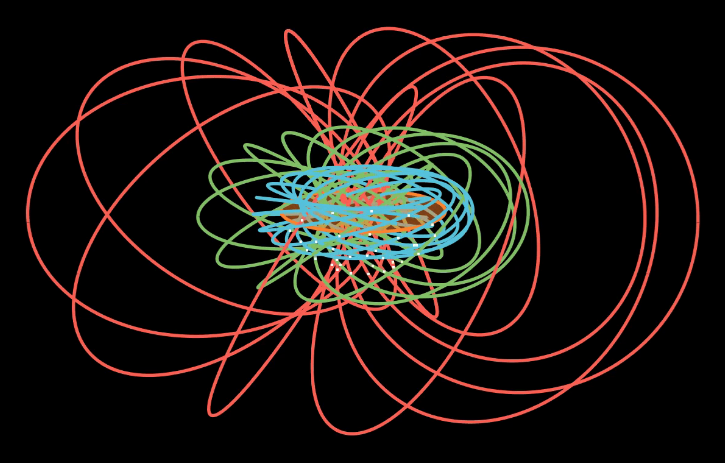
\includegraphics[width=0.92\textwidth,height=0.42\textheight,keepaspectratio]{fig0_1_hopf_linked_fibers.png}
  \caption{Figure 0.1 --- Linked Hopf fibers (stereographic view). Source: Kingdom Come \texttt{app/\allowbreak{}assets/\allowbreak{}home/\allowbreak{}hopf\_\allowbreak{}linked\_\allowbreak{}fibers.\allowbreak{}png}.}
  \label{fig:fig0-1-hopf-linked-fibers}
\end{figure}

\begin{quote}\small\textit{Figure 0.1.* Two (or more) fibers of the Hopf fibration after stereographic projection to \(\mathbb{R}^3\). Linking is the topological signature that will later underwrite \textbf{protection} of flux configurations: you cannot unlink fibers by continuous deformation without cutting.}\end{quote}

\begin{figure}[htbp]
  \centering
  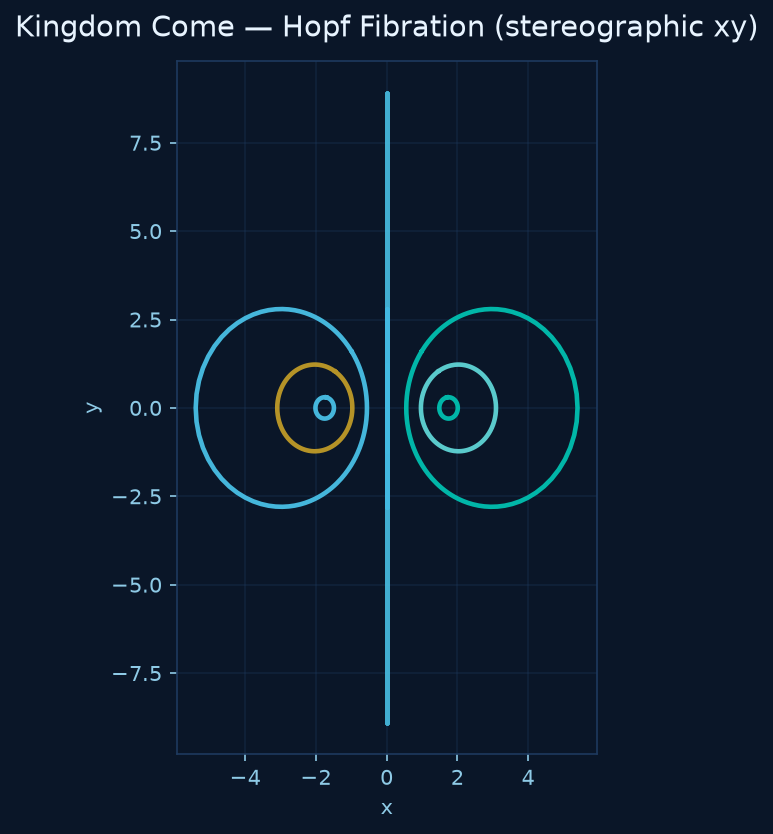
\includegraphics[width=0.92\textwidth,height=0.42\textheight,keepaspectratio]{fig0_2_hopf_stereographic.png}
  \caption{Figure 0.2 --- Stereographic Hopf preview. Source: Kingdom Come \texttt{app/\allowbreak{}assets/\allowbreak{}hopf\_\allowbreak{}preview.\allowbreak{}png}.}
  \label{fig:fig0-2-hopf-stereographic}
\end{figure}

\begin{quote}\small\textit{Figure 0.2.* A portal-style stereographic preview of the fibration: the same total space seen as a single composed picture rather than isolated fibers. In the Gradio app this is the ``Hopf Visualizer'' family of views (2D projections are preferred on CPU-only hosts).}\end{quote}

Hatcher's Farey diagram arranges \textbf{rational slopes} so that adjacency and mediants are visible. Hopf arranges \textbf{circle fibers} over a sphere so that linking and phase are visible. The analogy is not identity of objects; it is identity of \textbf{method}: a picture that makes the right discrete or continuous relationships obvious.

\textbf{Forward pointer.} Calling Hopf a ``Farey analogue'' is a \textbf{Model} metaphor only. \textbf{Chapter 3 will turn this metaphor into precise discrete definitions}---adjacency, mediants, and gauge data on a lattice in \(S^3\)---so that the analogy becomes a construction rather than a slogan.

\bigskip
\noindent\rule{\textwidth}{0.4pt}
\bigskip

\section{0.4 The Hopf fibration as a higher-dimensional Farey analogue}
\label{ch:ch00_preview:0-4-the-hopf-fibration-as-a-higher-dimensional-farey-analogu}

We state the comparison carefully so it does not pretend to be a theorem of uniqueness.

\begin{center}
\small
\setlength{\tabcolsep}{4pt}
\begin{tabularx}{\textwidth}{@{}>{\raggedright\arraybackslash}X>{\raggedright\arraybackslash}X@{}}
\toprule
Farey diagram (Hatcher) & Hopf geometry (this book) \\
\midrule
Vertices: rationals / cusps & Points of a discrete set in \(S^3\) (or in \(\mathbb{H}\)) \\
Edges: adjacency of fractions & Fiber segments / lattice bonds projecting under Hopf \\
Mediant of two fractions & Quaternionic (or lattice) combination rule, \textbf{to be axiomatized in Ch. 3} \\
Paths: continued fractions & Phase winding along fibers; walks on the gauged lattice \\
Symmetries: linear fractional maps & Left/right multiplication by unit quaternions; gauge actions \\
\bottomrule
\end{tabularx}
\end{center}


\begin{figure}[htbp]
  \centering
  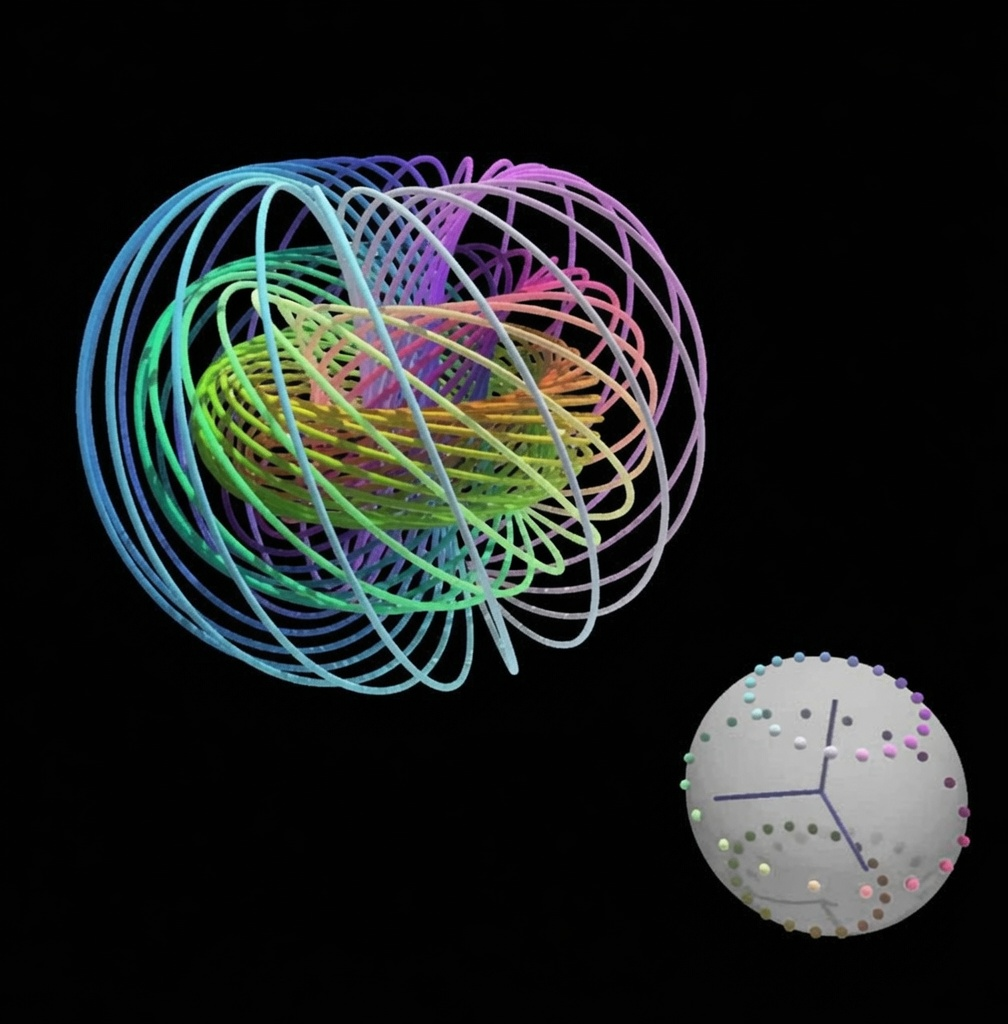
\includegraphics[width=0.92\textwidth,height=0.42\textheight,keepaspectratio]{fig0_3_hopf_bundle.png}
  \caption{Figure 0.3 --- Hopf fibration as a bundle. Source: Kingdom Come \texttt{app/\allowbreak{}assets/\allowbreak{}home/\allowbreak{}hopf\_\allowbreak{}fibration\_\allowbreak{}bundle.\allowbreak{}png}.}
  \label{fig:fig0-3-hopf-bundle}
\end{figure}

\begin{quote}\small\textit{Figure 0.3.* Conceptual bundle picture: total space \(S^3\), base \(S^2\), fibers circles. In Part II we \textbf{discretize} this picture---placing a lattice in the total space, projecting to the base, and defining adjacency---so that Farey-like combinatorial operations become available again.}\end{quote}

\textbf{Claim type:} Hopf fibration, linking, and the double cover \(\mathrm{Spin}(3)\to SO(3)\) via unit quaternions are \textbf{Theorems} of classical topology/geometry. Calling Hopf a ``Farey analogue'' remains a \textbf{Model} metaphor until Chapter 3 supplies the discrete axioms (see also Open Problem 1: \emph{canonical quaternionic Farey structure}).

\bigskip
\noindent\rule{\textwidth}{0.4pt}
\bigskip

\section{0.5 First sight of the gauged Hopf lattice and flux flywheels}
\label{ch:ch00_preview:0-5-first-sight-of-the-gauged-hopf-lattice-and-flux-flywheel}

Kingdom Come's physical \textbf{Model} (not yet a theorem of nature) can be stated in one paragraph:

> Physics emerges from \textbf{topologically protected flux structures} on a \textbf{gauged Hopf lattice} embedded in a \textbf{porous vacuum}. The Hopf fibration supplies the geometric backbone; quaternions supply the algebra; stable rotating configurations---\textbf{flux flywheels}---anchor emergent matter. Observer-linked phase holonomy between fibers damps toward synchrony with a coupling scale \(\kappa\).

A \textbf{flux flywheel}, for preview purposes, is a lattice-supported circulating flux whose topology (linking, winding, charge) obstructs continuous decay to a trivial configuration. In Hatcher's topographs, \textbf{periodicity} of separator lines produces infinite families of representations (Pell). Here, \textbf{periodicity of a flywheel} is the dynamical counterpart: a closed orbit of gauge and phase that refuses to unwind.

\begin{figure}[htbp]
  \centering
  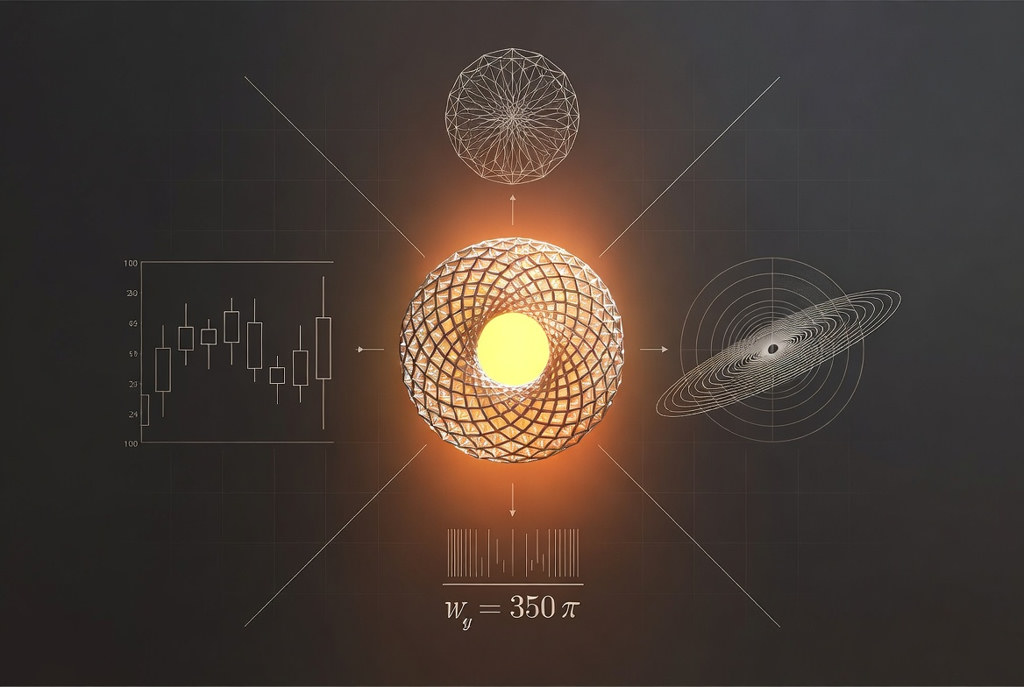
\includegraphics[width=0.92\textwidth,height=0.42\textheight,keepaspectratio]{fig0_4_flux_flywheel_scales.jpg}
  \caption{Figure 0.4 --- Flux flywheel scales. Source: Kingdom Come \texttt{app/\allowbreak{}assets/\allowbreak{}bitcoin\_\allowbreak{}pi/\allowbreak{}flux\_\allowbreak{}flywheel\_\allowbreak{}scales.\allowbreak{}jpg}.}
  \label{fig:fig0-4-flux-flywheel-scales}
\end{figure}

\begin{quote}\small\textit{Figure 0.4.* Nested / multi-scale flywheel imagery from the Kingdom Come observation assets. Read it as a \textbf{visual metaphor plus design sketch} for the lattice construction of Chapters 3--5: concentric scales, rotational identity, and coupling between levels. Formal definitions of lattice sites, gauge fields, and topological charge come later.}\end{quote}

In code, lattice and flywheel experiments live under:

\begin{itemize}
\item \texttt{kingdom.\allowbreak{}core.\allowbreak{}lattice} --- gauged lattice dynamics and stability comparisons  
\item \texttt{kingdom.\allowbreak{}core.\allowbreak{}flux\_\allowbreak{}flywheel} --- \texttt{map\_\allowbreak{}z\_\allowbreak{}to\_\allowbreak{}flywheel}, \texttt{map\_\allowbreak{}z\_\allowbreak{}to\_\allowbreak{}flywheel\_\allowbreak{}extended}  
\item Gradio tabs: \textbf{Lattice Simulator}, \textbf{Flux Flywheel}
\end{itemize}

Chapter 5 will introduce \textbf{flux topographs}: value landscapes for quaternionic (or lattice flux) functionals, the direct conceptual child of Conway topographs.

\bigskip
\noindent\rule{\textwidth}{0.4pt}
\bigskip

\section{0.6 A first \(Z\)-to-flux sketch and the \(350/\pi\) signature}
\label{ch:ch00_preview:0-6-a-first-z-to-flux-sketch-and-the-350-pi-signature}

\subsection{The \(Z\)-map (\textbf{Model})}
\label{ch:ch00_preview:the-z-map-model}

Kingdom Come implements a map from atomic number \(Z\) to a flywheel configuration and a bundle of stability / chemistry-facing metrics:

\[
Z \;\longmapsto\; \bigl(\text{flywheel state},\;\text{stability score},\;\text{shell-like descriptors},\;\ldots\bigr).
\]

Primary entry points: \texttt{map\_\allowbreak{}z\_\allowbreak{}to\_\allowbreak{}flywheel} and \texttt{map\_\allowbreak{}z\_\allowbreak{}to\_\allowbreak{}flywheel\_\allowbreak{}extended} in \texttt{kingdom.\allowbreak{}core.\allowbreak{}flux\_\allowbreak{}flywheel}. Detuning parameters (frequency offset, gauge strength, depth/layers) select \textbf{stability islands} in parameter space---\textbf{Magic Islands}---including a documented ultra-stable lock used as a noble-gas-like template.

The portal's element tour renders each \(Z\) with shell clouds and a flux ring. Two static stills from that tour are kept beside the main figures:

\begin{figure}[htbp]
  \centering
  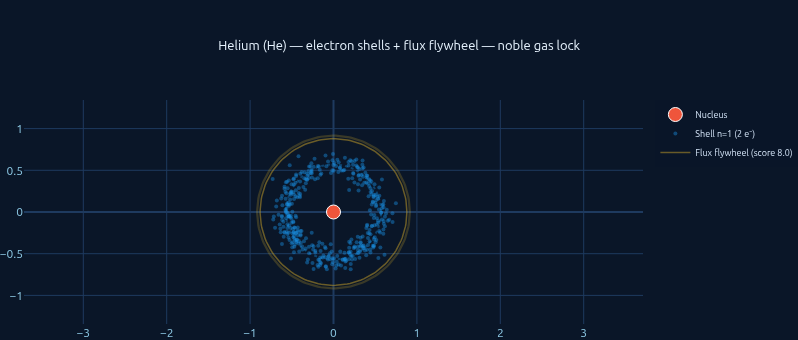
\includegraphics[width=0.92\textwidth,height=0.42\textheight,keepaspectratio]{aux_z_map_he.png}
  \caption{Auxiliary Figure A0.1 --- Helium (\(Z=2\)) flux-flywheel still: closed-shell archetype with high model stability. Source: Kingdom Come \texttt{z\_\allowbreak{}knowns/\allowbreak{}frame\_\allowbreak{}0002.\allowbreak{}png}.}
  \label{fig:aux-z-map-he}
\end{figure}

\begin{quote}\small\textit{Auxiliary Figure A0.1 --- Helium (\(Z=2\)).* Flux-flywheel element card from the portal tour: noble-gas closed shell, high stability score in the working model, and a simple shell/flux-ring visualization. Use this as the ``quiet baseline'' when comparing later \(Z\) values. Source: \texttt{z\_\allowbreak{}knowns/\allowbreak{}frame\_\allowbreak{}0002.\allowbreak{}png}.}\end{quote}

\begin{figure}[htbp]
  \centering
  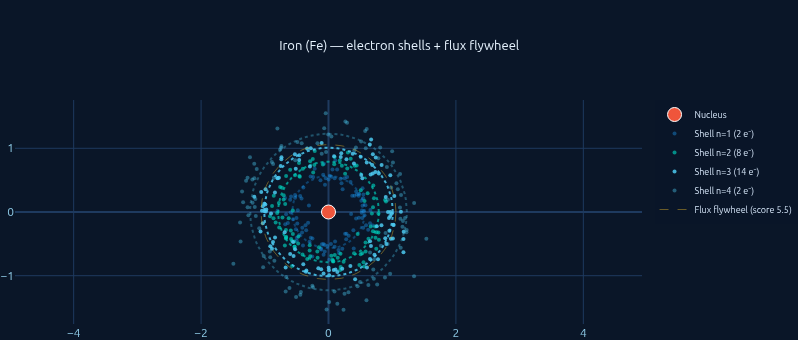
\includegraphics[width=0.92\textwidth,height=0.42\textheight,keepaspectratio]{aux_z_map_fe.png}
  \caption{Auxiliary Figure A0.2 --- Iron (\(Z=26\)) flux-flywheel still: mid-table nuclear/chemical specialness meets a richer flywheel profile. Source: Kingdom Come \texttt{z\_\allowbreak{}knowns/\allowbreak{}frame\_\allowbreak{}0026.\allowbreak{}png}.}
  \label{fig:aux-z-map-fe}
\end{figure}

\begin{quote}\small\textit{Auxiliary Figure A0.2 --- Iron (\(Z=26\)).* Same tour format at iron: a mid-table configuration where real-world nuclear and chemical specialness can later be checked against model metrics (stability, ionization-energy anchors, magnetic-moment proxies in Chapters 7 and 10). Source: \texttt{z\_\allowbreak{}knowns/\allowbreak{}frame\_\allowbreak{}0026.\allowbreak{}png}.}\end{quote}

\textbf{Claim type:} the existence of a coded map \(Z\mapsto\) configuration is a \textbf{Software fact}. Interpreting it as \emph{the} emergence mechanism of the periodic table is a \textbf{Model}. Quantitative alignment with experiment is an empirical research program (Chapters 7 and 10), not a free theorem.

\subsection{The \(350/\pi\) signature (\textbf{Hypothesis})}
\label{ch:ch00_preview:the-350-pi-signature-hypothesis}

Kingdom Come's constants module records a topological clock scale

\[
W_g \;=\; \frac{350}{\pi} \;\approx\; 111.408
\]

(\texttt{WG\_\allowbreak{}FROM\_\allowbreak{}350\_\allowbreak{}OVER\_\allowbreak{}PI}, with a documented lock value \(W_{g,\mathrm{lock}}\) in \texttt{flux\_\allowbreak{}hopf\_\allowbreak{}lib} / \texttt{kingdom.\allowbreak{}core.\allowbreak{}constants}). The same numerical motif appears in several \textbf{observation tracks} of the portal: Bitcoin Pi Cycle narratives, TLS tree branch bursts, cuprate superconductor sketches, pulsar-timing numerics, and related notes.

\begin{figure}[htbp]
  \centering
  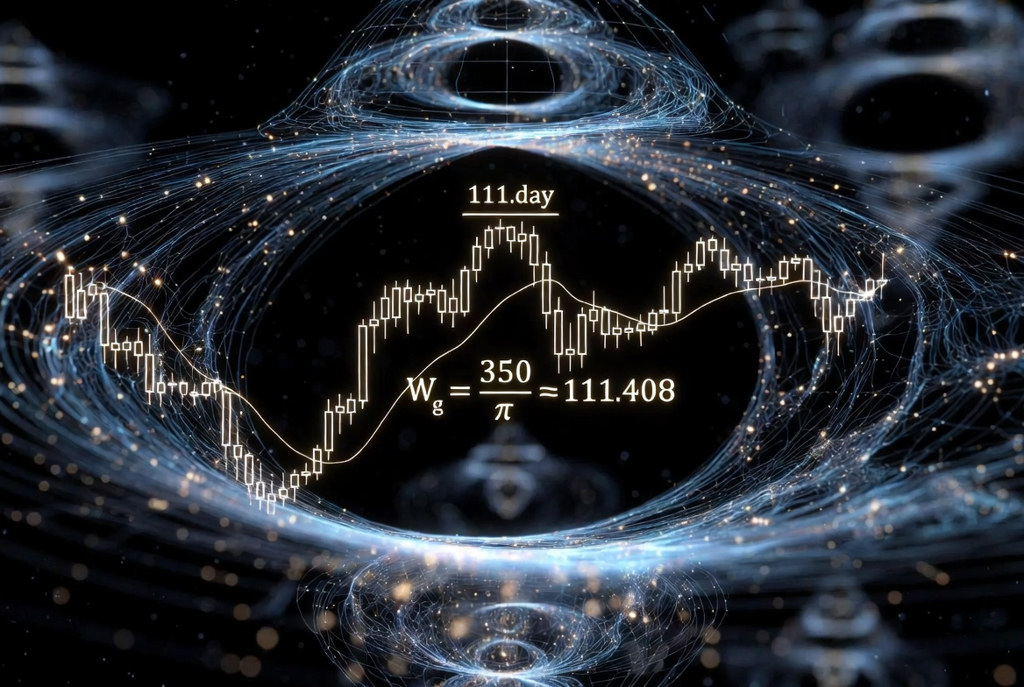
\includegraphics[width=0.92\textwidth,height=0.42\textheight,keepaspectratio]{fig0_5_hopf_lattice_pi_cycle.jpg}
  \caption{Figure 0.5 --- Hopf lattice and Pi-cycle motif. Source: Kingdom Come \texttt{app/\allowbreak{}assets/\allowbreak{}bitcoin\_\allowbreak{}pi/\allowbreak{}hopf\_\allowbreak{}lattice\_\allowbreak{}pi\_\allowbreak{}cycle.\allowbreak{}jpg}.}
  \label{fig:fig0-5-hopf-lattice-pi-cycle}
\end{figure}

\begin{quote}\small\textit{Figure 0.5.* Asset bridging the \textbf{gauged Hopf lattice} picture with the \(\pi\)-cycle / \(350/\pi\) observational storyline. In this book it marks the boundary between geometry (Parts I--IV) and the hypothesis layer (Part V).}\end{quote}

\textbf{Claim type: Hypothesis.} Recurrence of \(350/\pi\) across domains is \textbf{not} proved from first principles in this chapter. Chapter 10 will:

\begin{enumerate}
\item list each domain with source and method,  
\item require a statistical validation checklist,  
\item state what would \textbf{confirm, refine, or falsify} the hypothesis.
\end{enumerate}

Until then, treat \(W_g=350/\pi\) as a \textbf{named constant of the working model}, not as a theorem of number theory.

\bigskip
\noindent\rule{\textwidth}{0.4pt}
\bigskip

\section{0.7 Visual roadmap: Hatcher diagrams meet Hopf and Gradio}
\label{ch:ch00_preview:0-7-visual-roadmap-hatcher-diagrams-meet-hopf-and-gradio}

Think of the book as five floors of the same building:

\begin{lstlisting}[style=qga]
Part V   Ch. 10     Observations & validation     <- Hypothesis & Model
Part IV  Ch. 8-9    Class groups & algebras       <- Hatcher Ch. 7-8 lift
Part III Ch. 5-7    Forms, topographs, Z-map      <- Hatcher Ch. 4-6 lift
Part II  Ch. 3-4    Gauged lattice (Farey lift)   <- Hatcher Ch. 1-3 lift
Part I   Ch. 1-2    Quaternions & Hopf            <- foundations (new floor)
         Ch. 0      This preview
\end{lstlisting}

\textbf{How the five main figures will reappear}

\begin{center}
\small
\setlength{\tabcolsep}{4pt}
\begin{tabularx}{\textwidth}{@{}>{\raggedright\arraybackslash}X>{\raggedright\arraybackslash}X@{}}
\toprule
Figure & Returns in \\
\midrule
0.1 Linked fibers & Ch. 2 (definition, Hopf invariant); Ch. 4 (symmetry orbits) \\
0.2 Stereographic preview & Ch. 1--2 (coordinates, charts); Gradio labs \\
0.3 Bundle diagram & Ch. 2--3 (discrete total space / base) \\
0.4 Flywheel scales & Ch. 3, 5, 7 (lattice, topographs, \(Z\)-map) \\
0.5 Lattice / \(\pi\)-cycle & Ch. 3 (lattice); Ch. 10 (observations) \\
\bottomrule
\end{tabularx}
\end{center}


**Portal \(\leftrightarrow\) chapter cheat sheet**

\begin{center}
\small
\setlength{\tabcolsep}{4pt}
\begin{tabularx}{\textwidth}{@{}>{\raggedright\arraybackslash}X>{\raggedright\arraybackslash}X@{}}
\toprule
Gradio / module & First serious chapter \\
\midrule
Hopf Visualizer \(\cdot\) \texttt{core.\allowbreak{}hopf} \(\cdot\) \texttt{viz.\allowbreak{}hopf\_\allowbreak{}plotly} & 2 \\
Quaternion helpers \(\cdot\) \texttt{core.\allowbreak{}quaternion} & 1 \\
Lattice Simulator \(\cdot\) \texttt{core.\allowbreak{}lattice} & 3--4 \\
Flux Flywheel slider \(\cdot\) \texttt{core.\allowbreak{}flux\_\allowbreak{}flywheel} & 5--7 \\
Magic Island \(\cdot\) \texttt{viz.\allowbreak{}magic\_\allowbreak{}island} & 6 \\
Observations tabs \(\cdot\) \texttt{constants.\allowbreak{}WG\_\allowbreak{}FROM\_\allowbreak{}350\_\allowbreak{}OVER\_\allowbreak{}PI} & 10 \\
\bottomrule
\end{tabularx}
\end{center}


\bigskip
\noindent\rule{\textwidth}{0.4pt}
\bigskip

\section{0.8 Reading plan for the rest of the book}
\label{ch:ch00_preview:0-8-reading-plan-for-the-rest-of-the-book}

\begin{enumerate}
\item \textbf{Part I (Ch. 1--2)} makes quaternions algebraic and geometric, then defines the Hopf fibration carefully and rebuilds Figures 0.1--0.3 from first principles.  
\item \textbf{Part II (Ch. 3--4)} constructs the gauged Hopf lattice and its symmetries---the Farey lift (Open Problem 1).  
\item \textbf{Part III (Ch. 5--7)} develops forms, flux topographs, Magic Islands, and the \(Z\)-map as representation theory (Open Problems 2--4).  
\item \textbf{Part IV (Ch. 8--9)} treats composition, class groups, and quaternion algebras (Open Problem 6).  
\item \textbf{Part V (Ch. 10)} collects multi-domain observations (\(350/\pi\), \(Z\mapsto\) correlations, Magic Islands), states validation protocols (Table T4), and summarizes Open Problems OP1--OP6 (Open Problem 5).
\end{enumerate}

If you are impatient for physics, read 0 \(\rightarrow\) 2 \(\rightarrow\) 3 (flywheel sections) \(\rightarrow\) 7 \(\rightarrow\) 10, then return to fill the arithmetic spine. If you are a number theorist first, read 0--9 with Hatcher open, and treat Chapter 10 as a speculative appendix until the checklists are green.

\bigskip
\noindent\rule{\textwidth}{0.4pt}
\bigskip

\section{Exercises (preview level)}
\label{ch:ch00_preview:exercises-preview-level}

\textbf{0.A.} Verify \(N(q_1 q_2)=N(q_1)N(q_2)\) for two random integer quaternions by hand or with \texttt{kingdom.\allowbreak{}core.\allowbreak{}quaternion}.

\textbf{0.B.} In the Gradio Hopf Visualizer, load \textbf{Classic Hopf} and identify which panel corresponds most closely to Figure 0.1 versus Figure 0.2.

\textbf{0.C.} Run \texttt{map\_\allowbreak{}z\_\allowbreak{}to\_\allowbreak{}flywheel} for \(Z\in\{2,10,26,79\}\). Record stability scores; do \textbf{not} yet interpret them as chemical truth---only as model outputs.

\textbf{0.D.} Write one paragraph distinguishing \textbf{Theorem / Model / Hypothesis} for: (i) four-square theorem, (ii) Hopf linking, (iii) \(W_g=350/\pi\) as a multi-domain constant.

\textbf{0.E.} Open Hatcher TN Chapter 0 and list three pictures you expect to have quaternionic or Hopf analogues by the end of our Chapter 5.

\bigskip
\noindent\rule{\textwidth}{0.4pt}
\bigskip

\section{Code and asset pointers}
\label{ch:ch00_preview:code-and-asset-pointers}

\begin{lstlisting}[style=qga]
kingdom.core.quaternion      # Quaternion, from_hopf_coords, hopf_image
kingdom.core.hopf            # sample_fiber, sample_fiber_family
kingdom.core.lattice         # gauged lattice simulations
kingdom.core.flux_flywheel   # map_z_to_flywheel[_extended]
kingdom.core.constants       # WG_FROM_350_OVER_PI, W_G_LOCK, ? defaults
kingdom.viz.hopf_plotly      # portal-style multi-panel figures
\end{lstlisting}

\textbf{Figure sources (Kingdom Come):} see \texttt{figures/\allowbreak{}ATTRIBUTION.\allowbreak{}md}.

\textbf{Parallel reading:} Hatcher, \emph{Topology of Numbers}, Chapter 0; project file \texttt{HATCHER\_\allowbreak{}MAP.\allowbreak{}md}.

\bigskip
\noindent\rule{\textwidth}{0.4pt}
\bigskip



% Auto-generated from book/01_quaternions.md — do not edit by hand
% Regenerated by scripts/md_to_latex.py

\chapter{Chapter 1 --- Quaternions: Algebra, Geometry, and Arithmetic}
\label{ch:ch01_quaternions}

This chapter builds the algebraic and geometric language used everywhere later in the book. Chapter 2 fibers the unit sphere of quaternions; Chapters 3--4 act on it by left and right multiplication; later chapters repeatedly invoke norms, integer orders, and the four-square theorem.

\textbf{Learning goals}

\begin{enumerate}
\item Master the algebraic rules and geometric interpretation of quaternions.  
\item See unit quaternions as the three-sphere \(S^3\).  
\item Distinguish Lipschitz and Hurwitz orders and understand why the latter is preferred for arithmetic.  
\item Re-encounter the four-square theorem as a consequence of norm multiplicativity.  
\item Meet the double-cover relationship to three-dimensional rotations.  
\item Run first computational labs with \texttt{kingdom.core.quaternion}.
\end{enumerate}

\textbf{Figures in this chapter}

\begin{center}
\small
\begin{tabular}{@{}lp{0.28\textwidth}p{0.28\textwidth}@{}}
\toprule
Tag & File & Role \\
\midrule
Fig. 1.1 & \texttt{figures/fig1\_1\_ijk\_multiplication.png} & \(i,j,k\) cycle and multiplication table \\
Fig. 1.2 & \texttt{figures/fig1\_2\_s3\_unit\_quaternions.png} & Unit quaternions as \(S^3\subset\mathbb{R}^4\) \\
Fig. 1.3 & \texttt{figures/fig1\_3\_lipschitz\_hurwitz.png} & Lipschitz vs Hurwitz lattice (schematic) \\
Fig. 1.4 & \texttt{figures/fig1\_4\_norm\_multiplicativity.png} & Norm multiplicativity \(\rightarrow\) four squares \\
Aux A1.1 & \texttt{figures/aux1\_1\_quaternion\_rotation.png} & Rotation via \(v\mapsto qvq^{-1}\) (\(\rightarrow\) Ch. 2) \\
\bottomrule
\end{tabular}
\end{center}


\textbf{Claim discipline}

\begin{center}
\small
\begin{tabular}{@{}lp{0.55\textwidth}@{}}
\toprule
Claim & Type \\
\midrule
Algebra of \(\mathbb{H}\); \(N(q_1 q_2)=N(q_1)N(q_2)\); four-square theorem; \(\mathrm{Spin}(3)\to SO(3)\) double cover & \textbf{Theorem} (classical) \\
Preferring the Hurwitz order as the primary integer lattice for later flux/lattice work & \textbf{Model} choice \\
Kingdom Come / \texttt{flux\_hopf\_lib} APIs and demos & \textbf{Software fact} \\
\bottomrule
\end{tabular}
\end{center}


\bigskip
\noindent\rule{\textwidth}{0.4pt}
\bigskip

\section{1.1 Definition and basic operations}
\label{ch:ch01_quaternions:1-1-definition-and-basic-operations}

\subsection{The algebra \(\mathbb{H}\)}
\label{ch:ch01_quaternions:the-algebra-mathbb-h}

A \textbf{quaternion} is an expression

\[
q = a + bi + cj + dk,
\]

where \(a,b,c,d\in\mathbb{R}\) and the symbols \(i,j,k\) satisfy Hamilton's rules

\[
i^2 = j^2 = k^2 = ijk = -1.
\]

These force the cyclic products

\[
ij = k,\quad jk = i,\quad ki = j
\]

and the anticyclic products

\[
ji = -k,\quad kj = -i,\quad ik = -j.
\]

In particular, multiplication is \textbf{associative} and \textbf{distributive} over addition, but \textbf{not commutative}: \(ij\neq ji\).

As a real vector space,

\[
\mathbb{H} \;\cong\; \mathbb{R}^4,
\]

with basis \(\{1,i,j,k\}\). Addition and scalar multiplication are componentwise. The interesting structure is the bilinear product determined by the table above.

\begin{figure}[htbp]
  \centering
  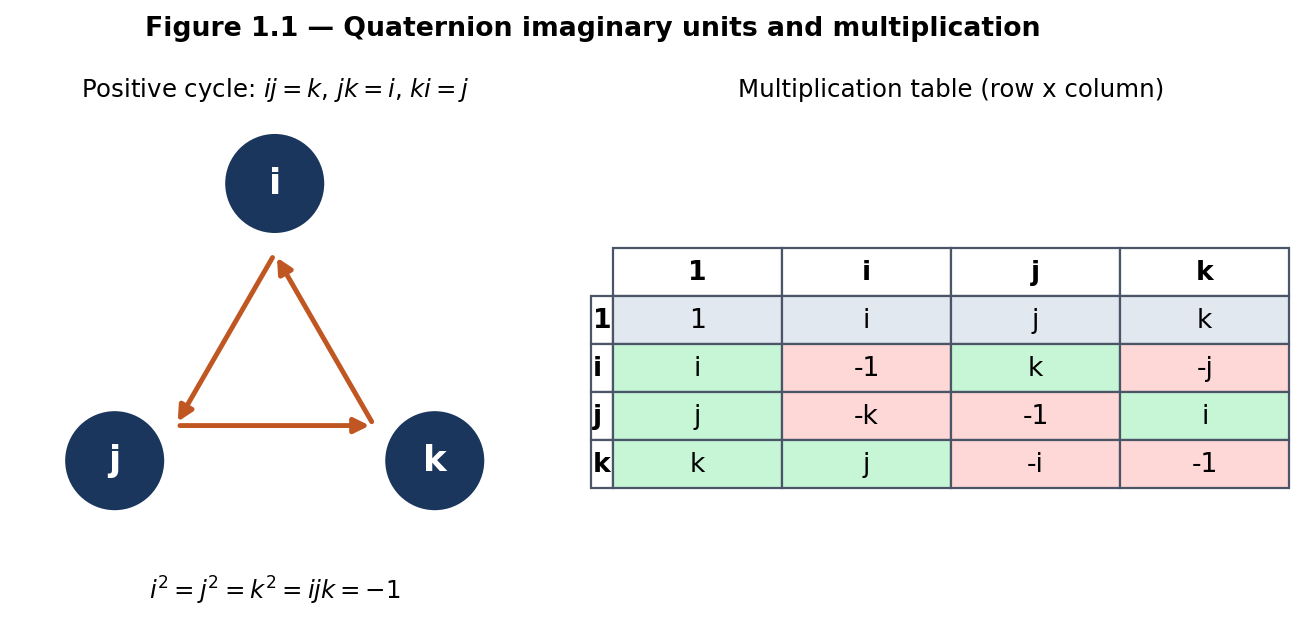
\includegraphics[width=0.92\textwidth,height=0.42\textheight,keepaspectratio]{fig1_1_ijk_multiplication.png}
  \caption{Figure 1.1 --- Quaternion imaginary units and multiplication table.}
  \label{fig:fig1-1-ijk-multiplication}
\end{figure}

\begin{quote}\small\textit{Figure 1.1.* Left: the positive cycle \(i\to j\to k\to i\). Right: the \(4\times 4\) multiplication table for \(\{1,i,j,k\}\). Red-tinted cells are negative results; green-tinted cells are the pure imaginary basis elements.}\end{quote}

\textbf{Notation.} We write \(q = (a,b,c,d)\) or \(q = a + \mathbf{v}\) with vector part \(\mathbf{v}=(b,c,d)\in\mathbb{R}^3\). Kingdom Come stores components as \texttt{(w, x, y, z)} with \(w=a\) the real part---the same convention as \texttt{flux\_hopf\_lib.quaternion.core.Quaternion}.

\subsection{Explicit product formula}
\label{ch:ch01_quaternions:explicit-product-formula}

If \(q_1 = a_1 + b_1 i + c_1 j + d_1 k\) and \(q_2 = a_2 + b_2 i + c_2 j + d_2 k\), then

\begin{align*}
q_1 q_2
&=
(a_1 a_2 - b_1 b_2 - c_1 c_2 - d_1 d_2)\\
&\quad+ (a_1 b_2 + b_1 a_2 + c_1 d_2 - d_1 c_2)\, i\\
&\quad+ (a_1 c_2 - b_1 d_2 + c_1 a_2 + d_1 b_2)\, j\\
&\quad+ (a_1 d_2 + b_1 c_2 - c_1 b_2 + d_1 a_2)\, k.
\end{align*}

This is exactly the formula implemented by \texttt{Quaternion.multiply} in both \texttt{flux\_hopf\_lib} and \texttt{kingdom.core.quaternion}.

\subsection{Complex pairs}
\label{ch:ch01_quaternions:complex-pairs}

Identifying \(\mathbb{C}\) with \(\mathrm{span}_{\mathbb{R}}\{1,i\}\) inside \(\mathbb{H}\), every quaternion can be written uniquely as

\[
q = z_1 + z_2\, j,\qquad z_1,z_2\in\mathbb{C},
\]

or as a pair \((z_1,z_2)\in\mathbb{C}^2\). This view is the natural bridge to the Hopf map in Chapter 2.

\bigskip
\noindent\rule{\textwidth}{0.4pt}
\bigskip

\section{1.2 Conjugation and the multiplicative norm}
\label{ch:ch01_quaternions:1-2-conjugation-and-the-multiplicative-norm}

\subsection{Conjugate}
\label{ch:ch01_quaternions:conjugate}

The \textbf{conjugate} of \(q = a + bi + cj + dk\) is

\[
\overline{q} = a - bi - cj - dk.
\]

Properties (all \textbf{Theorems}, elementary verifications):

\[
\overline{\overline{q}} = q,\qquad
\overline{q_1 + q_2} = \overline{q_1}+\overline{q_2},\qquad
\overline{q_1 q_2} = \overline{q_2}\,\overline{q_1}.
\]

Note the \textbf{order reversal} under conjugation of products---the noncommutative analogue of the complex rule \(\overline{zw}=\overline{z}\,\overline{w}\).

\subsection{Norm}
\label{ch:ch01_quaternions:norm}

The \textbf{(Euclidean) norm} is

\[
N(q) \;:=\; q\,\overline{q}
\;=\; a^2 + b^2 + c^2 + d^2
\;=\; |q|^2
\]

if one writes \(|q|\) for the Euclidean length in \(\mathbb{R}^4\). In code, \texttt{Quaternion.norm()} returns \(\sqrt{N(q)}=|q|\); the multiplicative quantity used in number theory is \(N(q)=|q|^2\). We will say \textbf{multiplicative norm} for \(N(q)\) and \textbf{length} for \(|q|\) when both appear.

\textbf{Theorem (multiplicativity of the norm).} For all \(q_1,q_2\in\mathbb{H}\),

\[
N(q_1 q_2) = N(q_1)\, N(q_2).
\]

\emph{Sketch.} \(N(q_1 q_2)=(q_1 q_2)\overline{(q_1 q_2)}=q_1 q_2 \overline{q_2}\,\overline{q_1}=q_1 N(q_2)\overline{q_1}=N(q_1)N(q_2)\), using that \(N(q_2)\) is real (hence central).

\begin{figure}[htbp]
  \centering
  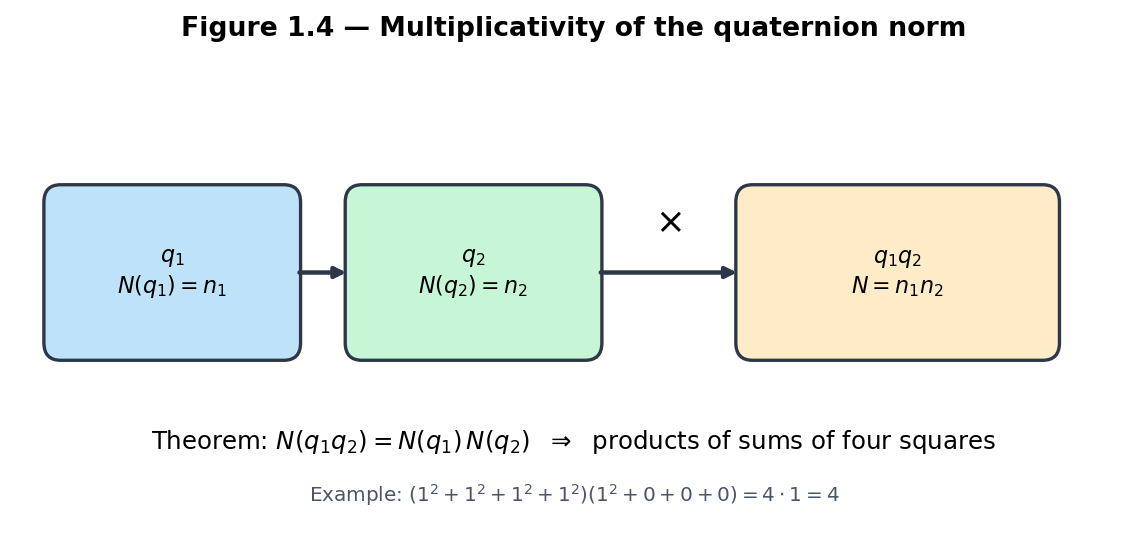
\includegraphics[width=0.92\textwidth,height=0.42\textheight,keepaspectratio]{fig1_4_norm_multiplicativity.png}
  \caption{Figure 1.4 --- Multiplicativity of the quaternion norm.}
  \label{fig:fig1-4-norm-multiplicativity}
\end{figure}

\begin{quote}\small\textit{Figure 1.4.* The product of two quaternions multiplies their norms. Every identity among sums of four squares is, at bottom, this theorem in arithmetic clothing.}\end{quote}

\subsection{Inverse}
\label{ch:ch01_quaternions:inverse}

If \(q\neq 0\), then

\[
q^{-1} = \frac{\overline{q}}{N(q)},
\]

so every nonzero quaternion is a unit in the division ring \(\mathbb{H}\). In floating-point code, \texttt{inverse()} divides by \(|q|^2\) and raises if \(|q|\) is near zero.

\bigskip
\noindent\rule{\textwidth}{0.4pt}
\bigskip

\section{1.3 Unit quaternions and the identification \(S^3\subset\mathbb{H}\cong\mathbb{R}^4\)}
\label{ch:ch01_quaternions:1-3-unit-quaternions-and-the-identification-s-3-subset-mathb}

\subsection{The three-sphere}
\label{ch:ch01_quaternions:the-three-sphere}

The set of \textbf{unit quaternions} is

\[
\mathrm{Sp}(1)
\;:=\;
\{ q\in\mathbb{H} : N(q)=1 \}
\;=\;
S^3 \subset \mathbb{R}^4.
\]

It is a compact Lie group under quaternion multiplication (associative, identity \(1\), inverses \(\overline{q}\)).

Geometrically:

\begin{itemize}
\item As a manifold, \(S^3\) is the unit sphere in four-dimensional Euclidean space.  
\item As a group, left (or right) multiplication by a fixed unit quaternion is an isometry of \(S^3\).  
\item As a complex pair, unit length means \(|z_1|^2+|z_2|^2=1\).
\end{itemize}

\begin{figure}[htbp]
  \centering
  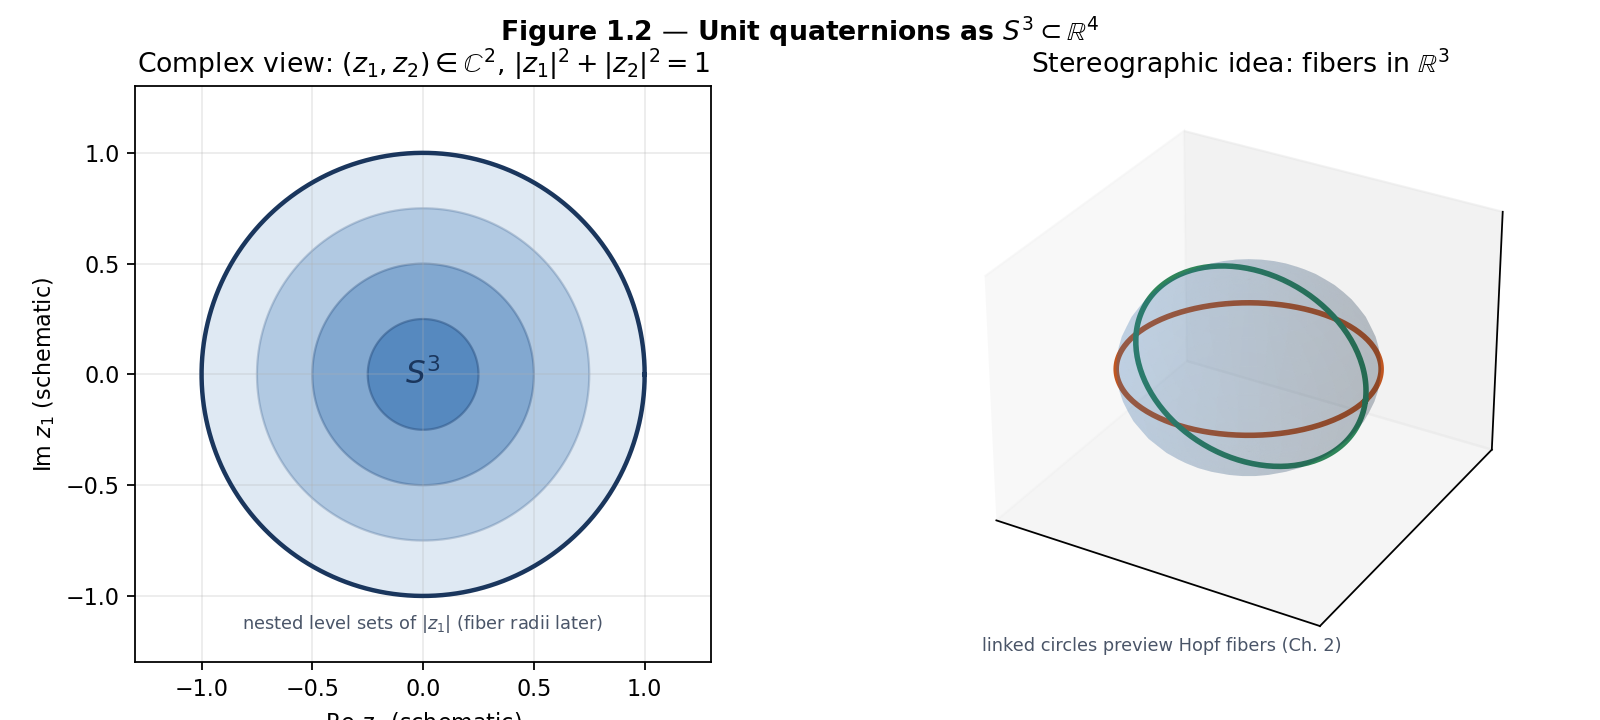
\includegraphics[width=0.92\textwidth,height=0.42\textheight,keepaspectratio]{fig1_2_s3_unit_quaternions.png}
  \caption{Figure 1.2 --- Unit quaternions as \(S^3\subset\mathbb{R}^4\).}
  \label{fig:fig1-2-s3-unit-quaternions}
\end{figure}

\begin{quote}\small\textit{Figure 1.2.* Left: schematic of the constraint \(|z_1|^2+|z_2|^2=1\) via nested level sets of \(|z_1|\). Right: after stereographic projection \(S^3\setminus\{\mathrm{pt}\}\to\mathbb{R}^3\), great-circle fibers will appear as linked circles (Chapter 2; compare Figs. 0.1--0.2).}\end{quote}

\subsection{Stereographic projection (preview)}
\label{ch:ch01_quaternions:stereographic-projection-preview}

Removing a point (classically \(-1\), or any fixed unit quaternion) and projecting to a tangent \(\mathbb{R}^3\) yields a global chart on \(S^3\setminus\{\mathrm{pt}\}\). Kingdom Come's Hopf visualizer uses stereographic (or orthographic 2D) projections heavily; here we only need that **\(S^3\) is drawable** once a chart is chosen. The full Hopf fibration story---fibers, linking, base \(S^2\)---is Chapter 2.

\subsection{Normalization in software}
\label{ch:ch01_quaternions:normalization-in-software}

\texttt{Quaternion.normalize()} returns \(q/|q|\) (or the identity if \(q\) is numerically zero). Portal methods that construct new quaternions return \texttt{type(self)} so subclass helpers such as \texttt{hopf\_image()} survive \texttt{normalize()} and \texttt{multiply()}.

\bigskip
\noindent\rule{\textwidth}{0.4pt}
\bigskip

\section{1.4 Integer quaternions: Lipschitz order vs Hurwitz order}
\label{ch:ch01_quaternions:1-4-integer-quaternions-lipschitz-order-vs-hurwitz-order}

\subsection{Lipschitz order}
\label{ch:ch01_quaternions:lipschitz-order}

The \textbf{Lipschitz order} is the set of quaternions with integer coordinates:

\[
L \;:=\; \mathbb{Z}[i,j,k]
\;=\;
\{ a+bi+cj+dk : a,b,c,d\in\mathbb{Z} \}.
\]

It is a free \(\mathbb{Z}\)-module of rank \(4\), closed under multiplication, and contains the eight \textbf{Lipschitz units}

\[
\{\pm 1,\pm i,\pm j,\pm k\}.
\]

Norms of Lipschitz quaternions are nonnegative integers. Multiplicativity still holds, so products of sums of four integer squares are again such sums.

\subsection{Hurwitz order}
\label{ch:ch01_quaternions:hurwitz-order}

The \textbf{Hurwitz order} \(\mathcal{H}\) consists of all quaternions whose coordinates are \textbf{either all integers or all half-integers}:

\[
\mathcal{H}
=
L \;\cup\;
\Bigl(\tfrac12 + \tfrac12 i + \tfrac12 j + \tfrac12 k + L\Bigr).
\]

Equivalently: \(a,b,c,d\in\mathbb{Z}\) or \(a,b,c,d\in\mathbb{Z}+\tfrac12\). This is still a ring (in fact a maximal order in the rational quaternion algebra \(\mathbb{H}_{\mathbb{Q}}\)), and it is \textbf{larger} than \(L\).

The unit group of \(\mathcal{H}\) has \textbf{24} elements---the binary tetrahedral group---including

\[
\pm 1,\;\pm i,\;\pm j,\;\pm k,\quad
\tfrac12(\pm 1\pm i\pm j\pm k)
\]

(all sign combinations). The extra units and lattice points make \(\mathcal{H}\) \textbf{Euclidean} with respect to the norm: for any \(q,d\in\mathcal{H}\) with \(d\neq 0\) there exist \(m,r\in\mathcal{H}\) with \(q = md + r\) and \(N(r)<N(d)\). That Euclidean property underwrites unique factorization phenomena used in classical proofs of the four-square theorem and in ideal theory (Chapter 9).

\begin{figure}[htbp]
  \centering
  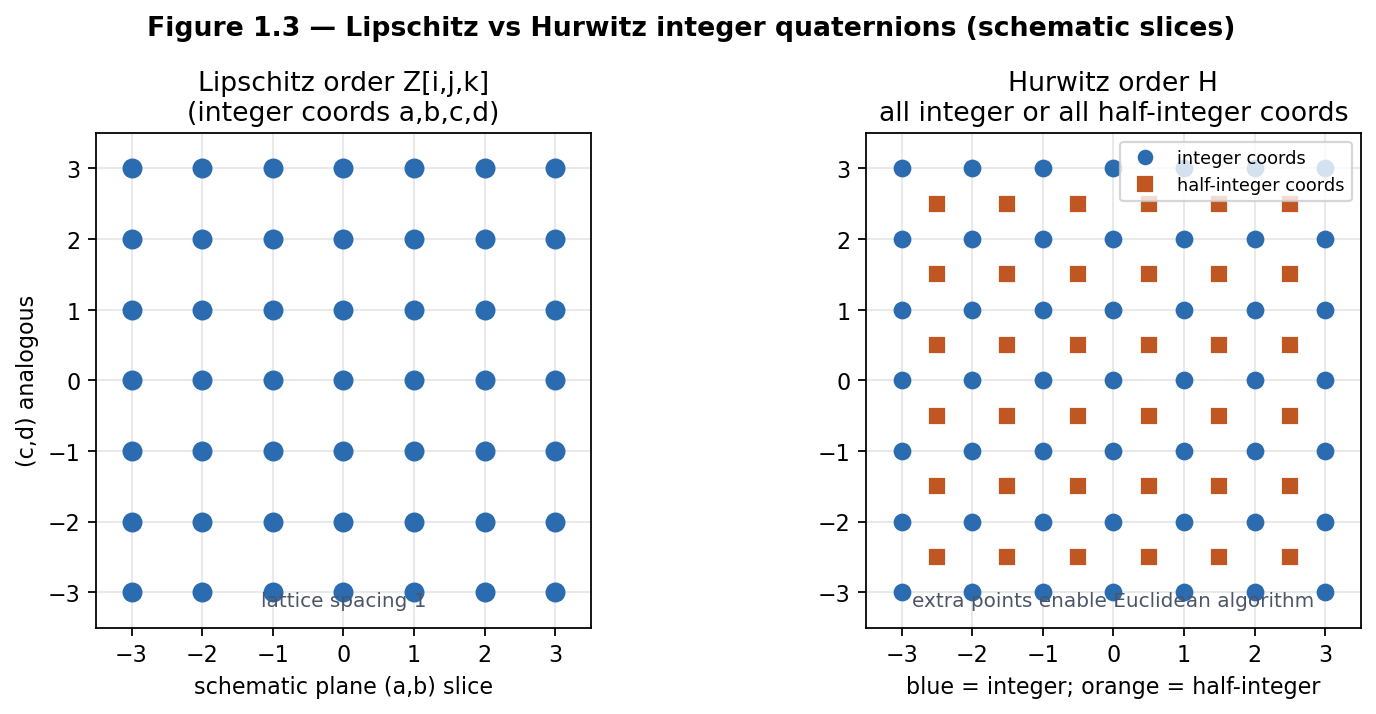
\includegraphics[width=0.92\textwidth,height=0.42\textheight,keepaspectratio]{fig1_3_lipschitz_hurwitz.png}
  \caption{Figure 1.3 --- Lipschitz vs Hurwitz (schematic slices).}
  \label{fig:fig1-3-lipschitz-hurwitz}
\end{figure}

\begin{quote}\small\textit{Figure 1.3.* Left: integer lattice (Lipschitz), shown in a 2D schematic slice. Right: Hurwitz adds half-integer points (orange squares) when all four coordinates share the same half-integer type. The picture is only a slice---true lattice geometry lives in \(\mathbb{R}^4\).}\end{quote}

\subsection{Why prefer Hurwitz later? (\textbf{Model})}
\label{ch:ch01_quaternions:why-prefer-hurwitz-later-model}

\begin{center}
\small
\begin{tabular}{@{}lp{0.28\textwidth}p{0.28\textwidth}@{}}
\toprule
Feature & Lipschitz \(L\) & Hurwitz \(\mathcal{H}\) \\
\midrule
Definition & Integer coords & Integer or half-integer coords \\
Units & 8 & 24 \\
Euclidean algorithm & fails in general & holds \\
Unique factorization flavor & weaker & stronger (classical) \\
Relation to four squares & works, clumsier proofs & clean norm arguments \\
\bottomrule
\end{tabular}
\end{center}


\textbf{Claim type: Model.} For the gauged Hopf lattice and flywheel arithmetic of Parts II--IV, this book \textbf{defaults to Hurwitz} (or to lattices containing \(\mathcal{H}\)) unless a section explicitly restricts to Lipschitz. That is a design choice aligned with classical quaternion number theory, not a theorem that Lipschitz is ``wrong.''

\textbf{Open thread.} Discrete adjacency rules built on \(\mathcal{H}\) (or on unit spheres over \(\mathcal{H}\)) feed Open Problem 1 in Chapter 3.

\bigskip
\noindent\rule{\textwidth}{0.4pt}
\bigskip

\section{1.5 The four-square theorem via norms}
\label{ch:ch01_quaternions:1-5-the-four-square-theorem-via-norms}

\textbf{Theorem (Lagrange).} Every natural number \(n\) is a sum of four integer squares:

\[
n = a^2 + b^2 + c^2 + d^2
\quad\text{for some }a,b,c,d\in\mathbb{Z}.
\]

\textbf{Quaternionic reading.} The statement is exactly: for every \(n\in\mathbb{N}\) there exists \(q\in L\) (Lipschitz) with \(N(q)=n\).

\textbf{Why multiplicativity matters.} Euler's four-square identity is \(N(q_1 q_2)=N(q_1)N(q_2)\) written in coordinates. Therefore it suffices to prove the theorem for primes (or for \(n\) square-free) and multiply representations. Classical proofs then show every prime is a norm from \(\mathcal{H}\) (or handle \(2\) and primes \(1\bmod 4\) / \(3\bmod 4\) by standard casework). Full proofs appear in many number-theory texts; Appendix D will collect a sketch. For this chapter, the essential message is:

> Four squares are not an isolated curiosity---they are the \textbf{norm theory of integer quaternions}.

\textbf{Comparison with Hatcher.} Hatcher's early chapters revolve around \textbf{two} squares and binary quadratic forms (Gaussian integers, topographs, class groups). Quaternions are the four-dimensional upgrade: the same geometric instinct (norms, units, lattices), one dimension higher. Chapter 5 will lift topographs themselves.

\textbf{Claim type: Theorem} (classical). No new proof is claimed here.

\bigskip
\noindent\rule{\textwidth}{0.4pt}
\bigskip

\section{1.6 Quaternions as rotations: the double cover \(\mathrm{Spin}(3)\to SO(3)\)}
\label{ch:ch01_quaternions:1-6-quaternions-as-rotations-the-double-cover-mathrm-spin-3-}

\subsection{Conjugation action on pure imaginaries}
\label{ch:ch01_quaternions:conjugation-action-on-pure-imaginaries}

Identify \(\mathbb{R}^3\) with the pure imaginary quaternions

\[
\mathrm{Im}\,\mathbb{H} = \{ bi + cj + dk : b,c,d\in\mathbb{R} \}.
\]

For a \textbf{unit} quaternion \(q\in S^3\) and \(v\in\mathrm{Im}\,\mathbb{H}\), set

\[
\rho_q(v) \;:=\; q\, v\, q^{-1} = q\, v\, \overline{q}.
\]

Then \(\rho_q(v)\) is again pure imaginary, and \(\rho_q\) is an orthogonal linear map of \(\mathbb{R}^3\) with determinant \(+1\). Thus we obtain a homomorphism

\[
\rho: S^3 \longrightarrow SO(3),\qquad q\mapsto \rho_q.
\]

\subsection{Axis--angle formula}
\label{ch:ch01_quaternions:axis-angle-formula}

If \(q = \cos(\theta/2) + \sin(\theta/2)\, u\) with unit pure imaginary \(u\) (i.e. \(u^2=-1\)), then \(\rho_q\) is rotation by angle \(\theta\) about the axis \(u\). This is the content of Rodrigues' formula; Kingdom Come exposes both \texttt{Quaternion.from\_axis\_angle(axis, theta)} and \texttt{rodrigues\_rotation}.

\begin{figure}[htbp]
  \centering
  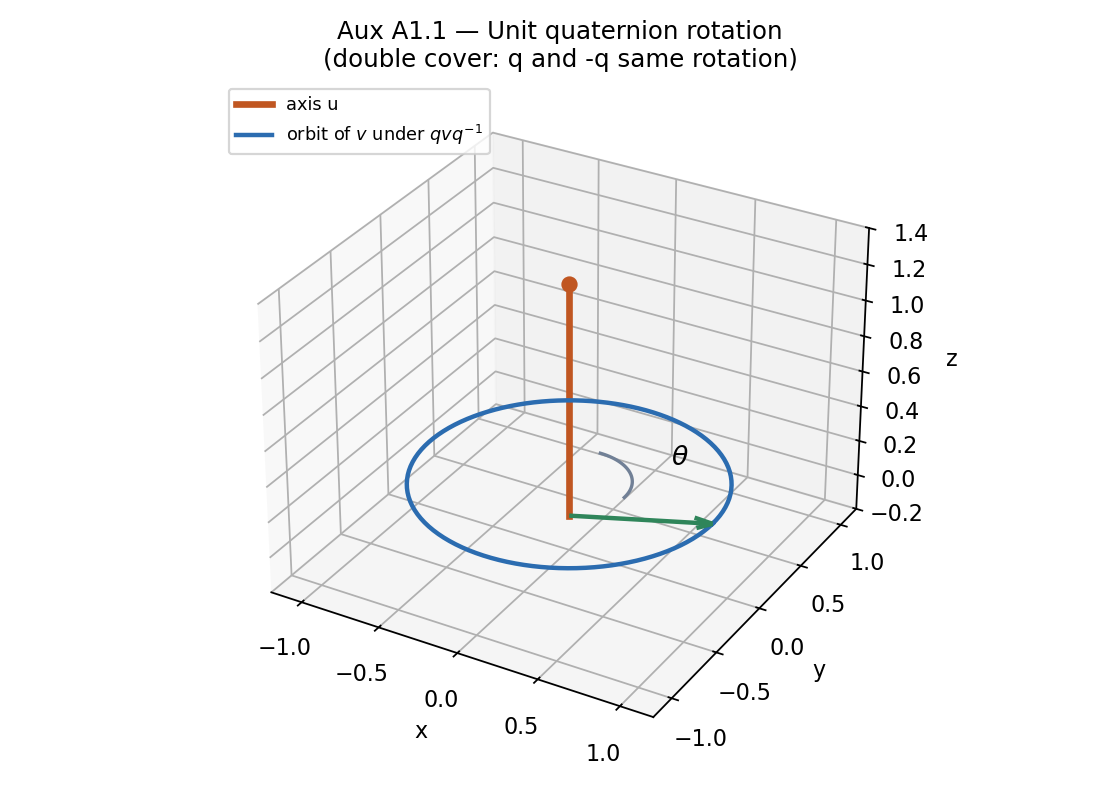
\includegraphics[width=0.92\textwidth,height=0.42\textheight,keepaspectratio]{aux1_1_quaternion_rotation.png}
  \caption{Auxiliary Figure A1.1 --- Unit quaternion rotation \(v\mapsto qvq^{-1}\).}
  \label{fig:aux1-1-quaternion-rotation}
\end{figure}

\begin{quote}\small\textit{Auxiliary Figure A1.1.* A vector \(v\) swept around an axis \(u\) under the conjugation action of a one-parameter family of unit quaternions. The same rotation arises from \(q\) and from \(-q\).}\end{quote}

\subsection{The kernel is \(\{\pm 1\}\)}
\label{ch:ch01_quaternions:the-kernel-is-pm-1}

Clearly \(\rho_{-q}=\rho_q\), since \((-q)v(-q)^{-1}=qvq^{-1}\). In fact

\[
\ker\rho = \{\pm 1\},
\]

so \(\rho\) is a \textbf{2-to-1} covering homomorphism

\[
S^3 \;\cong\; \mathrm{Spin}(3) \;\longrightarrow\; SO(3).
\]

Topologically this is the unique nontrivial double cover of \(SO(3)\). Paths in \(SO(3)\) that rotate by \(2\pi\) lift to paths in \(S^3\) from \(q\) to \(-q\); only a \(4\pi\) rotation closes in the cover---the origin of spinorial sign changes in physics.

\textbf{Claim type: Theorem} (classical Lie theory / geometry).

\textbf{Forward link.} The same unit quaternions that rotate \(\mathbb{R}^3\) will, in Chapter 2, be points of the \textbf{total space} of the Hopf fibration. Left and right multiplications that preserve the fibration become the symmetry language of Chapters 3--4.

\bigskip
\noindent\rule{\textwidth}{0.4pt}
\bigskip

\section{1.7 First computational examples and labs}
\label{ch:ch01_quaternions:1-7-first-computational-examples-and-labs}

Core API: \texttt{kingdom.core.quaternion} (see also Appendix C ?C.1).

\textbf{Labs (short form).} Full listings: \textbf{Appendix C}.

\begin{itemize}
\item \textbf{1.A} Verify \(ij=k\), \(ji=-k\), \(i^2=-1\) with \texttt{Quaternion}.
\item \textbf{1.B} Check \(N(q_1q_2)=N(q_1)N(q_2)\) numerically (residual \(\sim 10^{-14}\)).
\item \textbf{1.C} Enumerate small Lipschitz norms.
\item \textbf{1.D} Confirm \(q\) and \(-q\) induce the same conjugation action on a pure vector.
\item \textbf{1.E} Optional: \texttt{from\_hopf\_coords} / \texttt{hopf\_image} (preview of Ch. 2).
\end{itemize}

\begin{lstlisting}[style=qga,language=python]
from kingdom.core.quaternion import Quaternion
i, j = Quaternion(0,1,0,0), Quaternion(0,0,1,0)
print(i.multiply(j))  # k
\end{lstlisting}

\bigskip
\noindent\rule{\textwidth}{0.4pt}
\bigskip

\section{Exercises}
\label{ch:ch01_quaternions:exercises}

\textbf{1.A (hand).} Expand \((a+bi+cj+dk)(e+fi+gj+hk)\) and match the formula in ?1.1.

\textbf{1.B (hand).} Prove \(\overline{q_1 q_2}=\overline{q_2}\,\overline{q_1}\) from the multiplication table (or from the explicit formula).

\textbf{1.C (hand).} Show that \(N(q)=q\overline{q}\) is real and nonnegative, and that \(N(q)=0\Leftrightarrow q=0\).

\textbf{1.D (hand).} Verify that the 24 Hurwitz units listed in ?1.4 all have norm \(1\). How many Lipschitz units are among them?

\textbf{1.E (hand / reading).} Using multiplicativity, show that if \(n=N(q_1)\) and \(m=N(q_2)\) then \(nm=N(q_1 q_2)\). Explain in one sentence why this reduces Lagrange's theorem to representing primes.

\textbf{1.F (hand).} Let \(q=\cos(\theta/2)+\sin(\theta/2)\,i\). Compute \(q\, j\, \overline{q}\) and identify the rotation in the \(jk\)-plane.

\textbf{1.G (code).} Complete Labs 1.A--1.D. Submit residuals for Lab 1.B and a printed set of norms for Lab 1.C with \(N_{\max}=3\).

\textbf{1.H (code).} Using \texttt{chordal\_distance} (upstream) or \(\min(|q-r|,|q+r|)\), verify numerically that \(q\) and \(-q\) are close in the rotation sense even when far in \(\mathbb{R}^4\).

\textbf{1.I (Hatcher bridge).} In Hatcher, sums of two squares and Gaussian integers organize binary quadratic forms. Write three sentences mapping: (Gaussian integers \(\leftrightarrow\) Lipschitz/Hurwitz), (complex modulus \(\leftrightarrow\) quaternion norm), (unit circle \(S^1\) \(\leftrightarrow\) unit quaternions \(S^3\)).

\textbf{1.J (forward).} Without reading Chapter 2, guess: if unit quaternions are points of \(S^3\), what might a natural map \(S^3\to S^2\) do to a whole circle of phases? (You will check your guess against the Hopf map next.)

\bigskip
\noindent\rule{\textwidth}{0.4pt}
\bigskip

\section{Code and asset pointers}
\label{ch:ch01_quaternions:code-and-asset-pointers}

\begin{lstlisting}[style=qga]
kingdom.core.quaternion.Quaternion
kingdom.core.quaternion.rodrigues_rotation
flux_hopf_lib.quaternion.core.Quaternion   # upstream implementation
flux_hopf_lib.quaternion.core.q_mult, q_conj, q_normalize
\end{lstlisting}

\textbf{Figures:} generated for this chapter under \texttt{book/figures/fig1\_*} and \texttt{aux1\_1\_*} (see \texttt{FIGURES.md}). \textbf{Related portal:} Gradio rotation intuition is secondary here; Hopf Visualizer becomes primary in Chapter 2.

\bigskip
\noindent\rule{\textwidth}{0.4pt}
\bigskip

\section{Looking ahead}
\label{ch:ch01_quaternions:looking-ahead}

With the algebraic and geometric language of quaternions in hand---product, conjugate, norm, \(S^3\), Hurwitz arithmetic, and the double cover of \(SO(3)\)---we are ready to \textbf{fiber} \(S^3\) over \(S^2\) in Chapter 2. The same unit quaternions will reappear as total-space points; their left and right multiplications will become the symmetries of the gauged Hopf lattice in Part II.

\bigskip
\noindent\rule{\textwidth}{0.4pt}
\bigskip



% Auto-generated from book/02_hopf.md — do not edit by hand
% Regenerated by scripts/md_to_latex.py

\chapter{Chapter 2 --- The Hopf Fibration}
\label{ch:ch02_hopf}

This chapter defines the Hopf fibration from first principles and rebuilds the visual intuition of Figures 0.1--0.3. The same unit quaternions introduced in Chapter 1 become the total space \(S^3\). Left and right multiplications on this total space will become the symmetry language of the gauged Hopf lattice in Chapters 3--4.

\textbf{Learning goals}

\begin{enumerate}
\item Define the Hopf fibration in both complex-pair and real four-vector coordinates.  
\item Understand the fibers as circles and see their linking (Hopf invariant \(1\)).  
\item Work with stereographic projections and the visualizations used throughout the book.  
\item Recognize the bundle structure and basic charts.  
\item Connect the fibration back to unit quaternions and forward to the discrete lattice.  
\item Run labs with \texttt{kingdom.core.hopf} and the Gradio Hopf Visualizer.
\end{enumerate}

\textbf{Figures in this chapter}

\begin{center}
\small
\begin{tabular}{@{}lp{0.28\textwidth}p{0.28\textwidth}@{}}
\toprule
Tag & File & Role \\
\midrule
Fig. 2.1 & \texttt{figures/fig2\_1\_hopf\_definition.png} & Hopf map diagram (total space \(\rightarrow\) base) \\
Fig. 2.2 & \texttt{figures/fig2\_2\_linked\_fibers.png} & Linked Hopf fibers (stereographic) --- rebuild of Fig. 0.1 \\
Fig. 2.3 & \texttt{figures/fig2\_3\_stereographic\_preview.png} & Multi-panel stereographic preview --- rebuild of Fig. 0.2 \\
Fig. 2.4 & \texttt{figures/fig2\_4\_bundle\_structure.png} & Total space \(\rightarrow\) base with fibers --- rebuild of Fig. 0.3 \\
Aux A2.1 & \texttt{figures/aux2\_1\_fiber\_phase\_sweep.png} & Single fiber phase sweep \\
Aux A2.2 & \texttt{figures/aux2\_2\_hopf\_charts.png} & Local charts on base \(S^2\) \\
\bottomrule
\end{tabular}
\end{center}


\textbf{Claim discipline}

\begin{center}
\small
\begin{tabular}{@{}lp{0.55\textwidth}@{}}
\toprule
Claim & Type \\
\midrule
Hopf fibration definition, fiber structure, linking (Hopf invariant \(=1\)); double cover \(\mathrm{Spin}(3)\to SO(3)\) from Ch. 1 & \textbf{Theorem} (classical differential topology / geometry) \\
Interpreting the Hopf fibration as a higher-dimensional ``Farey analogue'' for the gauged lattice & \textbf{Model} \\
Kingdom Come visualizations and \texttt{kingdom.core.hopf} / \texttt{flux\_hopf\_lib} implementations & \textbf{Software fact} \\
\bottomrule
\end{tabular}
\end{center}


\bigskip
\noindent\rule{\textwidth}{0.4pt}
\bigskip

\section{2.1 Definition of the Hopf fibration}
\label{ch:ch02_hopf:2-1-definition-of-the-hopf-fibration}

\subsection{Complex-pair form (standard in the literature)}
\label{ch:ch02_hopf:complex-pair-form-standard-in-the-literature}

Identify unit quaternions with pairs of complex numbers (Chapter 1):

\[
q = z_1 + z_2\, j \quad \longleftrightarrow \quad (z_1, z_2) \in \mathbb{C}^2,
\qquad |z_1|^2 + |z_2|^2 = 1.
\]

One classical form of the \textbf{Hopf map} \(h: S^3 \to S^2\) is

\[
h(z_1, z_2)
=
\bigl(
  |z_1|^2 - |z_2|^2,\;
  2\,\mathrm{Re}(\overline{z_1} z_2),\;
  2\,\mathrm{Im}(\overline{z_1} z_2)
\bigr)
\in S^2 \subset \mathbb{R}^3,
\]

or, equivalently, the projectivized ratio

\[
[z_1 : z_2] \in \mathbb{CP}^1 \cong S^2.
\]

The second description makes the \textbf{circle fiber} obvious: multiplying \((z_1,z_2)\) by a common phase \(e^{i\phi}\) does not change the projective point.

\subsection{Real four-vector form (Kingdom Come / \texttt{flux\_hopf\_lib})}
\label{ch:ch02_hopf:real-four-vector-form-kingdom-come-flux-hopf-lib}

For a unit 4-vector \((x_1,x_2,x_3,x_4)\in S^3\), the library implements

\begin{align*}
y_1 &= x_1^2 - x_2^2,\\
y_2 &= 2\, x_1 x_2,\\
y_3 &= 2\,(x_3 x_4 + x_1 x_2),
\end{align*}

followed by Euclidean normalization so that \((y_1,y_2,y_3)\in S^2\). Quaternion components are identified as

\[
(w,x,y,z) \;\equiv\; (x_1,x_2,x_3,x_4).
\]

This is the form documented in Kingdom Come's theory notes and used by \texttt{hopf\_map}, \texttt{hopf\_map\_quaternion}, and \texttt{Quaternion.hopf\_image()}.

\textbf{Convention note (software vs textbook).} The classical complex form and the portal's real four-vector formula are \textbf{both} maps \(S^3\to S^2\) in the Hopf family of constructions, but they need not agree componentwise under a fixed identification of \(\mathbb{R}^3\) coordinates. Labs in this chapter treat the \textbf{library formula as the working computational standard} for Kingdom Come continuity, while the complex \(\mathbb{CP}^1\) description remains the cleanest \textbf{Theorem}-level definition of fibers (common phase \(e^{i\phi}\)). When proving linking or Hopf invariant \(1\), use the classical bundle; when plotting portal-compatible curves, use \texttt{sample\_fiber} / \texttt{hopf\_map}.

\textbf{Angle coordinates.} The library also uses Hopf angles \((\eta,\xi_1,\xi_2)\) via \texttt{hopf\_coordinates}:

\begin{align*}
x_1 &= \cos\eta\,\cos\xi_1, &
x_2 &= \cos\eta\,\sin\xi_1,\\
x_3 &= \sin\eta\,\cos\xi_2, &
x_4 &= \sin\eta\,\sin\xi_2,
\end{align*}

with \(\eta\in[0,\pi/2]\) (or a practical subrange) and \(\xi_1,\xi_2\in[0,2\pi)\). Fixing \((\eta,\xi_1)\) and sweeping \(\xi_2\) traces a \textbf{fiber}.

\begin{figure}[htbp]
  \centering
  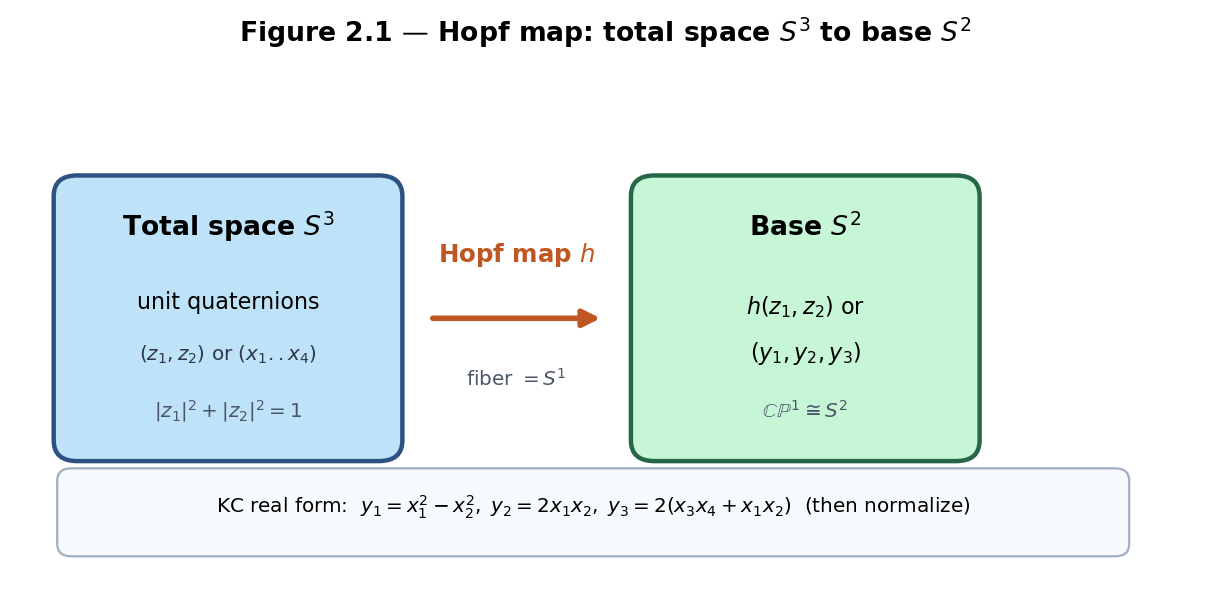
\includegraphics[width=0.92\textwidth,height=0.42\textheight,keepaspectratio]{fig2_1_hopf_definition.png}
  \caption{Figure 2.1 --- Hopf map definition.}
  \label{fig:fig2-1-hopf-definition}
\end{figure}

\begin{quote}\small\textit{Figure 2.1.* From total space \(S^3\) (unit quaternions) to base \(S^2\). The map is smooth and surjective; every base point has a circle's worth of preimages.}\end{quote}

\textbf{API note (Software fact).} Call signatures in code are component-wise, not `\texttt{pass a Quaternion object'' to }hopf\_map`:

\begin{lstlisting}[style=qga]
hopf_map(x1, x2, x3, x4)           -> (y1, y2, y3)
hopf_map_quaternion(w, x, y, z)    -> (y1, y2, y3)
Quaternion(...).hopf_image()       -> (y1, y2, y3)
\end{lstlisting}

\bigskip
\noindent\rule{\textwidth}{0.4pt}
\bigskip

\section{2.2 Fibers and linking}
\label{ch:ch02_hopf:2-2-fibers-and-linking}

\subsection{Fibers are circles}
\label{ch:ch02_hopf:fibers-are-circles}

Over each point \(p\in S^2\) the preimage \(h^{-1}(p)\) is diffeomorphic to a circle \(S^1\). In angle coordinates, that circle is parametrized by the fiber phase \(\xi_2\) at fixed base coordinates \((\eta,\xi_1)\). In the complex picture, it is the \(U(1)\) action

\[
(z_1,z_2) \;\longmapsto\; (e^{i\phi} z_1,\; e^{i\phi} z_2).
\]

\subsection{Linking and the Hopf invariant}
\label{ch:ch02_hopf:linking-and-the-hopf-invariant}

Any two distinct fibers are \textbf{linked exactly once} in \(S^3\). After stereographic projection to \(\mathbb{R}^3\), this appears as linked Villarceau circles on nested tori. The classical \textbf{Hopf invariant} of the map \(h: S^3\to S^2\) equals \(1\).

Linking is the topological feature that later underwrites \textbf{topological protection} of flux configurations on the gauged lattice: continuous deformations that preserve the fiber structure cannot unlink configurations without a cut or a singular transition.

\begin{figure}[htbp]
  \centering
  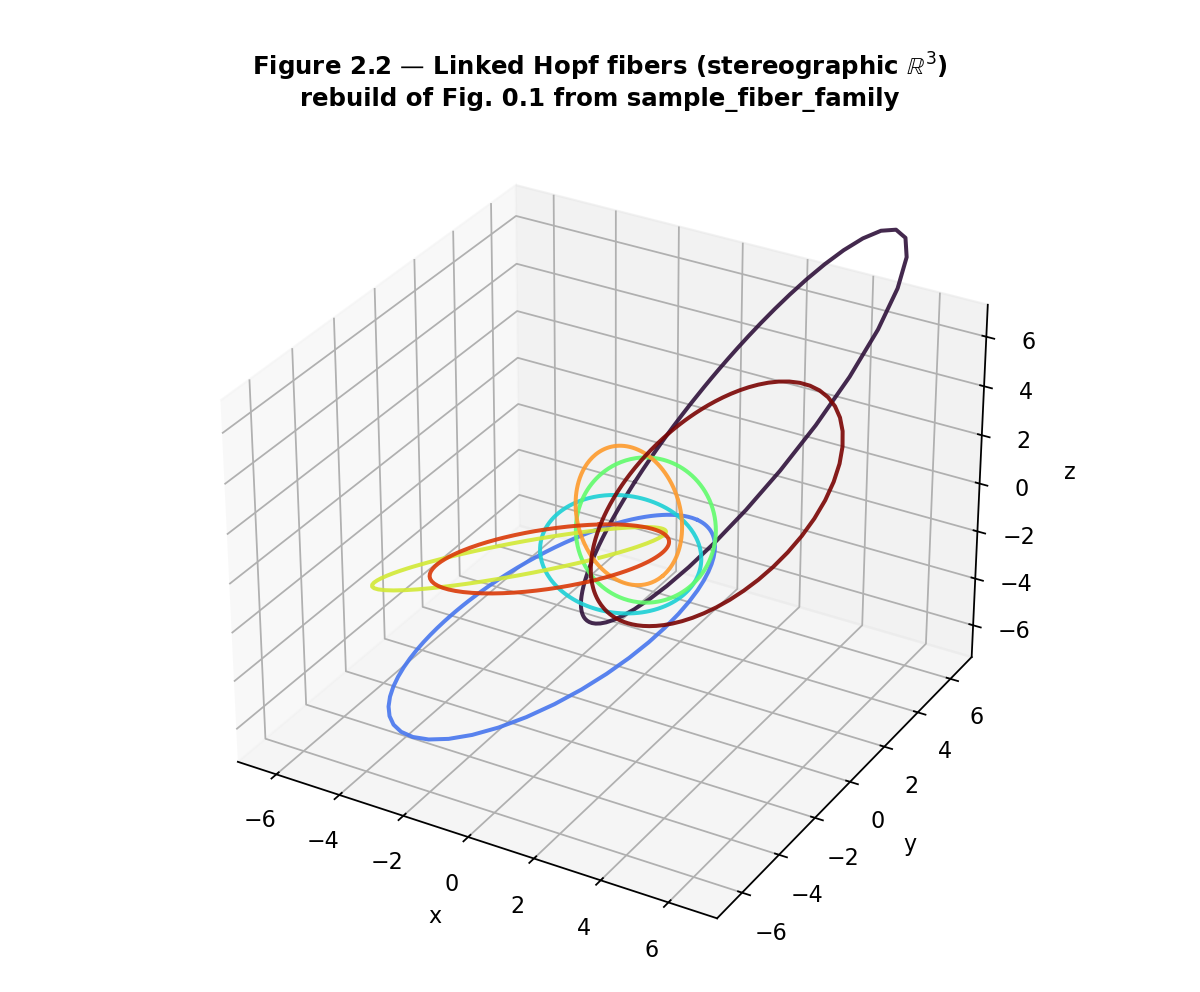
\includegraphics[width=0.92\textwidth,height=0.42\textheight,keepaspectratio]{fig2_2_linked_fibers.png}
  \caption{Figure 2.2 --- Linked Hopf fibers (stereographic view).}
  \label{fig:fig2-2-linked-fibers}
\end{figure}

\begin{quote}\small\textit{Figure 2.2.* Rebuild of Figure 0.1, generated from \texttt{sample\_fiber\_family}. Several fibers after stereographic projection \(S^3\setminus\{\mathrm{pt}\}\to\mathbb{R}^3\). Linking cannot be undone by continuous deformation without cutting a fiber.}\end{quote}

\textbf{Claim type: Theorem.} Fiber structure and Hopf invariant \(=1\) are classical results in differential topology.

\textbf{Software diagnostics.} The library exposes linking helpers (\texttt{linking\_number\_pair}, \texttt{fiber\_linking\_number}, \texttt{fiber\_pair\_diagnostics}) for numerical checks on sampled curves---useful in labs, not substitutes for the classical theorem.

\bigskip
\noindent\rule{\textwidth}{0.4pt}
\bigskip

\section{2.3 Stereographic projections and visualizations}
\label{ch:ch02_hopf:2-3-stereographic-projections-and-visualizations}

\subsection{Projection formula}
\label{ch:ch02_hopf:projection-formula}

Kingdom Come / \texttt{flux\_hopf\_lib} use a stereographic chart with pole related to the fourth coordinate (TOE-compatible convention):

\[
(x_1,x_2,x_3,x_4)
\;\longmapsto\;
\Bigl(
  \frac{s\, x_2}{1-x_4},\;
  \frac{s\, x_3}{1-x_4},\;
  \frac{s\, x_1}{1-x_4}
\Bigr),
\]

with default scale \(s=2\) (\texttt{stereographic\_project}). Fibers map to closed curves in \(\mathbb{R}^3\).

\subsection{Portal layout}
\label{ch:ch02_hopf:portal-layout}

The Gradio \textbf{Hopf Visualizer} defaults to multi-panel \textbf{2D} views (xy, xz, phase map, \(S^2\) base markers) for CPU-only hosts, with optional 3D WebGL modes locally. That multi-panel layout is the live counterpart of Figure 2.3.

\begin{figure}[htbp]
  \centering
  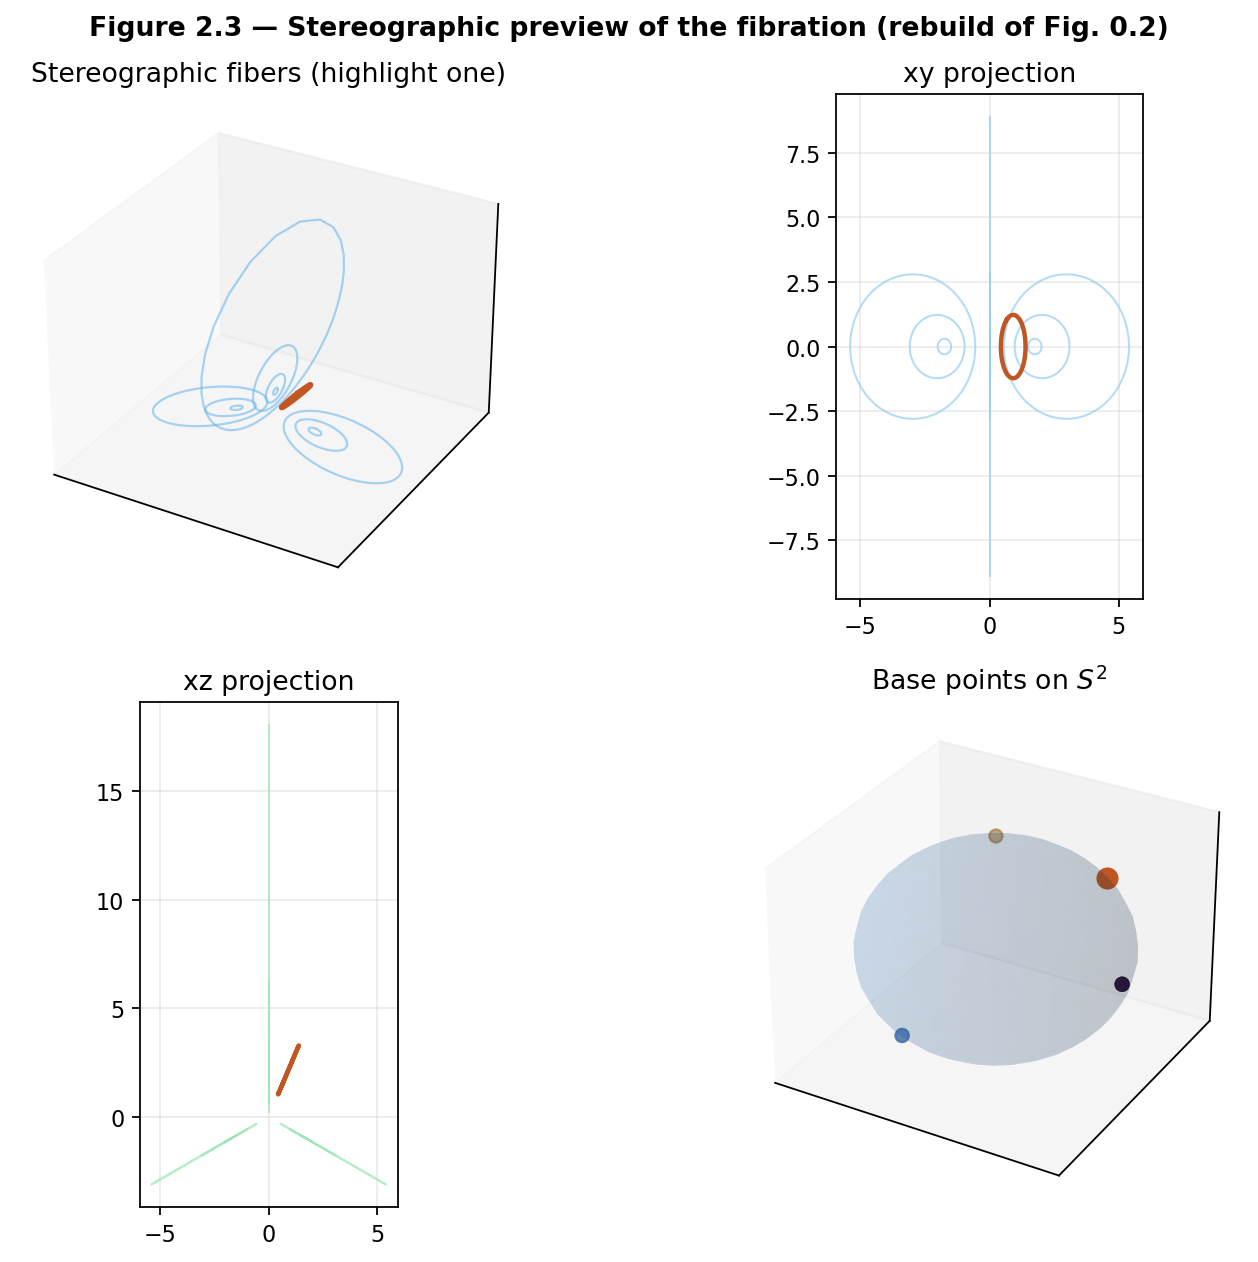
\includegraphics[width=0.92\textwidth,height=0.42\textheight,keepaspectratio]{fig2_3_stereographic_preview.png}
  \caption{Figure 2.3 --- Stereographic preview of the fibration.}
  \label{fig:fig2-3-stereographic-preview}
\end{figure}

\begin{quote}\small\textit{Figure 2.3.* Rebuild of Figure 0.2. Composed stereographic fibers, planar projections, and base points on \(S^2\), with one fiber highlighted---the same visual language as the portal's Classic Hopf preset.}\end{quote}

\textbf{Sampling API (Software fact).} \texttt{sample\_fiber(eta, xi1, n\_points=...)} returns a \textbf{dictionary}, not a bare list of quaternions:

\[
\{\texttt{eta},\;\texttt{xi1},\;\texttt{xi2},\;
\texttt{x1..x4},\;\texttt{y1..y3},\;
\texttt{px,py,pz},\;
\texttt{base\_y1..base\_y3},\;\ldots\}.
\]

\texttt{sample\_fiber\_family(...)} returns a list of such dictionaries over a spread of base points.

\bigskip
\noindent\rule{\textwidth}{0.4pt}
\bigskip

\section{2.4 Bundle structure and charts}
\label{ch:ch02_hopf:2-4-bundle-structure-and-charts}

\subsection{Fiber bundle}
\label{ch:ch02_hopf:fiber-bundle}

The Hopf fibration is a fiber bundle

\[
S^1 \;\hookrightarrow\; S^3 \;\twoheadrightarrow\; S^2.
\]

It is the canonical example of a nontrivial principal \(U(1)\)-bundle (equivalently, an \(S^1\)-bundle). Locally it is a product \(U\times S^1\); globally the twisting produces the linking of fibers.

\begin{figure}[htbp]
  \centering
  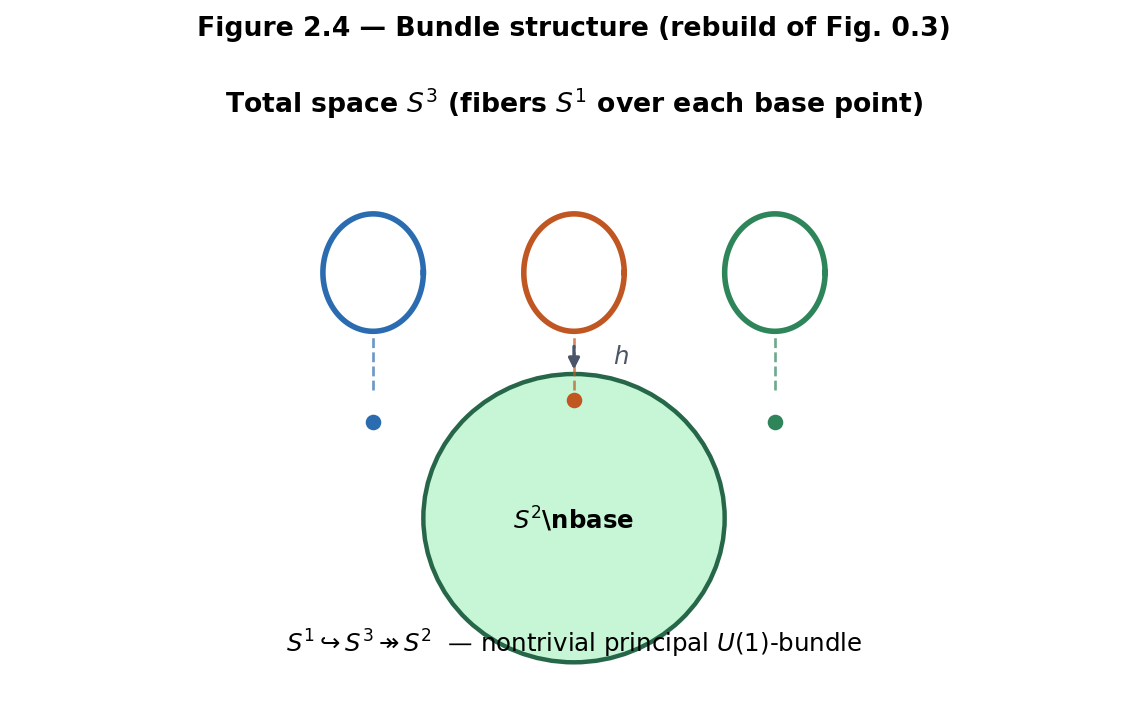
\includegraphics[width=0.92\textwidth,height=0.42\textheight,keepaspectratio]{fig2_4_bundle_structure.png}
  \caption{Figure 2.4 --- Bundle picture: total space, fibers, base.}
  \label{fig:fig2-4-bundle-structure}
\end{figure}

\begin{quote}\small\textit{Figure 2.4.* Rebuild of Figure 0.3. Conceptual diagram of the bundle structure that Chapter 3 will \textbf{discretize}: lattice points in the total space, Hopf projection to the base, adjacency and gauge along fibers.}\end{quote}

\subsection{Local charts on the base}
\label{ch:ch02_hopf:local-charts-on-the-base}

The base \(S^2\) is covered by the usual stereographic charts (north and south). Over each chart \(U\subset S^2\) there is a local trivialization

\[
h^{-1}(U) \;\cong\; U \times S^1,
\]

so a fiber coordinate (phase) can be chosen continuously on \(U\). Crossing from one chart to another changes the phase by a transition function valued in \(U(1)\)---the seed of \textbf{gauge} language for Part II.

\begin{figure}[htbp]
  \centering
  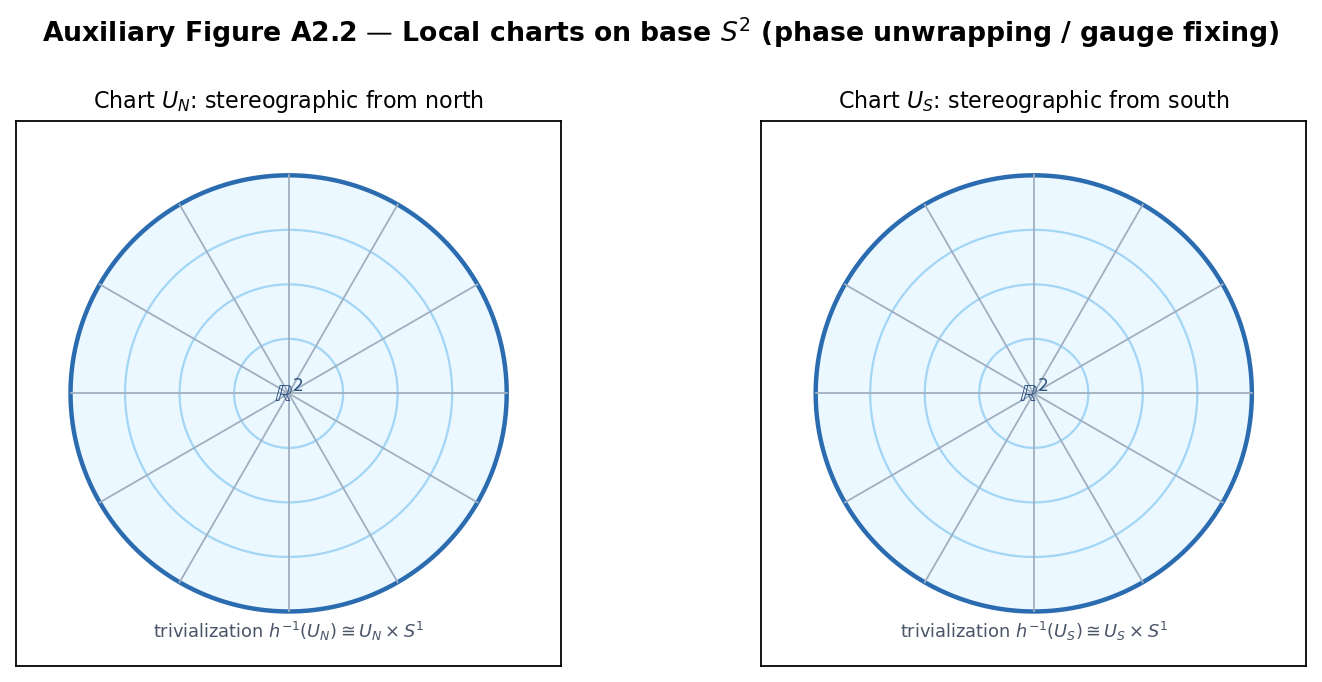
\includegraphics[width=0.92\textwidth,height=0.42\textheight,keepaspectratio]{aux2_2_hopf_charts.png}
  \caption{Auxiliary Figure A2.2 --- Local charts on base \(S^2\).}
  \label{fig:aux2-2-hopf-charts}
\end{figure}

\begin{quote}\small\textit{Auxiliary Figure A2.2.* Schematic north/south charts on the base. Phase unwrapping and gauge fixing on the discrete lattice will live over such charts.}\end{quote}

\subsection{Phase sweep along a fiber}
\label{ch:ch02_hopf:phase-sweep-along-a-fiber}

Holding the base point fixed and varying the fiber phase is the continuous analogue of ``walking in the fiber direction.'' In Hatcher's Farey world, continued-fraction paths walk along edges of a planar diagram; here the primitive closed walk is a fiber circle.

\begin{figure}[htbp]
  \centering
  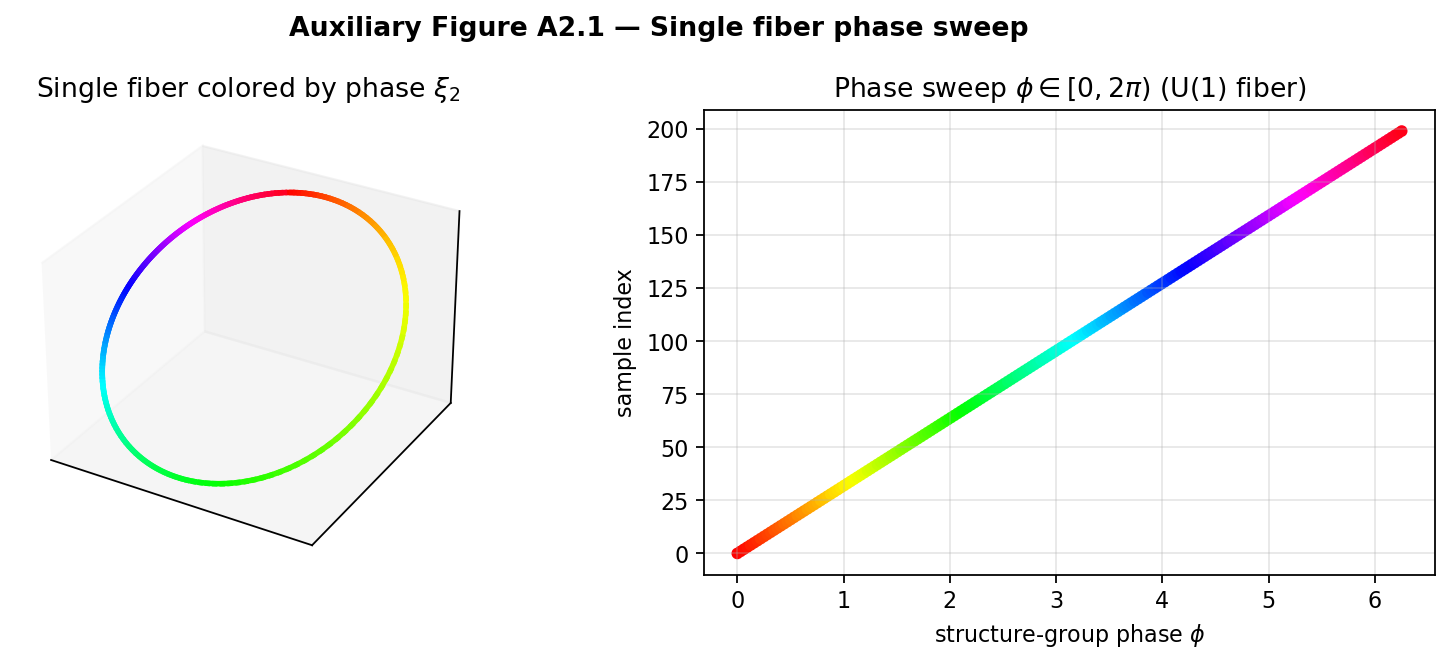
\includegraphics[width=0.92\textwidth,height=0.42\textheight,keepaspectratio]{aux2_1_fiber_phase_sweep.png}
  \caption{Auxiliary Figure A2.1 --- Single fiber phase sweep.}
  \label{fig:aux2-1-fiber-phase-sweep}
\end{figure}

\begin{quote}\small\textit{Auxiliary Figure A2.1.* One fiber colored by phase \(\xi_2\in[0,2\pi)\). The path closes: a full sweep returns to the same unit quaternion (up to sampling).}\end{quote}

\textbf{Model reminder.} Calling Hopf a higher-dimensional ``Farey analogue'' remains a \textbf{Model} metaphor until Chapter 3 axiomatizes discrete adjacency and mediants on the gauged lattice (Open Problem 1).

\bigskip
\noindent\rule{\textwidth}{0.4pt}
\bigskip

\section{2.5 Connection to quaternions and rotations}
\label{ch:ch02_hopf:2-5-connection-to-quaternions-and-rotations}

\subsection{Every unit quaternion lies on exactly one fiber}
\label{ch:ch02_hopf:every-unit-quaternion-lies-on-exactly-one-fiber}

The Hopf map partitions \(S^3\) into fibers. Chapter 1's unit group \(\mathrm{Sp}(1)=S^3\) is therefore a circle bundle over \(S^2\).

\subsection{Left and right multiplications}
\label{ch:ch02_hopf:left-and-right-multiplications}

If \(u\in S^3\) is fixed:

\begin{itemize}
\item \textbf{Left multiplication} \(q\mapsto uq\) is an isometry of \(S^3\). It maps fibers to fibers and induces a rotation of the base \(S^2\).  
\item \textbf{Right multiplication} \(q\mapsto qu\) is also an isometry; its interaction with fibers is different (fiberwise phase and the classical identification of right \(U(1)\) with the structure group of the bundle, in the complex picture).
\end{itemize}

Together, left and right actions generate the symmetry repertoire we will \textbf{gauge} and discretize in Chapters 3--4. The double cover \(\mathrm{Spin}(3)\to SO(3)\) from ?1.6 sits naturally here: directions in \(\mathbb{R}^3\) relate to the base, while the fiber phase is the extra spinorial degree of freedom.

\textbf{Claim type: Theorem} for the continuous group actions and bundle structure; \textbf{Model} for their later role as lattice gauge symmetries.

\bigskip
\noindent\rule{\textwidth}{0.4pt}
\bigskip

\section{2.6 First computational labs}
\label{ch:ch02_hopf:2-6-first-computational-labs}

Core entry points:

\begin{lstlisting}[style=qga]
kingdom.core.hopf.hopf_map
kingdom.core.hopf.hopf_map_quaternion
kingdom.core.hopf.hopf_coordinates
kingdom.core.hopf.sample_fiber
kingdom.core.hopf.sample_fiber_family
kingdom.core.hopf.stereographic_project
kingdom.core.quaternion.Quaternion.hopf_image
kingdom.core.quaternion.Quaternion.from_hopf_coords
kingdom.viz.hopf_plotly
\end{lstlisting}

\subsection{Lab 2.A --- Hopf image of a unit quaternion}
\label{ch:ch02_hopf:lab-2-a-hopf-image-of-a-unit-quaternion}

\begin{lstlisting}[style=qga,language=python]
from kingdom.core.quaternion import Quaternion

q = Quaternion(0.5, 0.5, 0.5, 0.5).normalize()
y = q.hopf_image()
print(y)
print(sum(c * c for c in y) ** 0.5)  # ~ 1
\end{lstlisting}

Equivalent component form:

\begin{lstlisting}[style=qga,language=python]
from kingdom.core.hopf import hopf_map_quaternion

print(hopf_map_quaternion(q.w, q.x, q.y, q.z))
\end{lstlisting}

\subsection{Lab 2.B --- Sample a fiber}
\label{ch:ch02_hopf:lab-2-b-sample-a-fiber}

\begin{lstlisting}[style=qga,language=python]
from kingdom.core.hopf import sample_fiber
import numpy as np

fiber = sample_fiber(eta=0.4, xi1=0.3, n_points=64)
print(fiber.keys())
# library records a representative base point from the first sample
print(fiber["base_y1"], fiber["base_y2"], fiber["base_y3"])
# stereographic curve in R^3
print(fiber["px"][:3], fiber["py"][:3], fiber["pz"][:3])
# S^3 samples should have unit length
X = np.stack([fiber["x1"], fiber["x2"], fiber["x3"], fiber["x4"]], axis=1)
print(np.linalg.norm(X, axis=1)[:5])  # ~ 1
# closed loop in R^3: endpoints nearly meet after full phase (endpoint=False)
p0 = np.array([fiber["px"][0], fiber["py"][0], fiber["pz"][0]])
p_near = np.array([fiber["px"][-1], fiber["py"][-1], fiber["pz"][-1]])
print("endpoint gap (stereo):", np.linalg.norm(p0 - p_near))
\end{lstlisting}

\textbf{Note.} \texttt{sample\_fiber} sweeps \(\xi_2\) at fixed \((\eta,\xi_1)\) and returns stereographic curves used throughout the portal. For a textbook check that a true classical fiber lies over one \(\mathbb{CP}^1\) point, apply a common complex phase to a fixed \((z_1,z_2)\) (Exercise 2.C) rather than expecting bit-identical constancy of every real-component convention.

\subsection{Lab 2.C --- Visualize in the portal style}
\label{ch:ch02_hopf:lab-2-c-visualize-in-the-portal-style}

Open the Gradio \textbf{Hopf Visualizer} tab, load \textbf{Classic Hopf}, and identify:

\begin{enumerate}
\item which panel is the **base \(S^2\)** markers,  
\item which panels are \textbf{linked-fiber projections} (xy / xz),  
\item which panel (if present) is a \textbf{phase} view.
\end{enumerate}

Compare with Figures 2.2--2.3.

\subsection{Lab 2.D --- Phase sweep on one fiber}
\label{ch:ch02_hopf:lab-2-d-phase-sweep-on-one-fiber}

\begin{lstlisting}[style=qga,language=python]
from kingdom.core.hopf import sample_fiber
import numpy as np

fiber = sample_fiber(eta=0.55, xi1=0.2, n_points=200)
# phase closes: first and last sample are neighbors on the circle
p0 = np.array([fiber["px"][0], fiber["py"][0], fiber["pz"][0]])
p1 = np.array([fiber["px"][-1], fiber["py"][-1], fiber["pz"][-1]])
# with endpoint=False sampling, last point is just before return
p_return = np.array([fiber["px"][0], fiber["py"][0], fiber["pz"][0]])
chord = np.linalg.norm(
    np.array([fiber["x1"][0], fiber["x2"][0], fiber["x3"][0], fiber["x4"][0]])
    - np.array([fiber["x1"][-1], fiber["x2"][-1], fiber["x3"][-1], fiber["x4"][-1]])
)
print("chord between first and last sample on S^3:", chord)
print("xi2 range:", fiber["xi2"][0], "->", fiber["xi2"][-1])
\end{lstlisting}

Optionally animate \texttt{xi2} in a notebook or use portal phase controls. Auxiliary Figure A2.1 is the static version of this lab.

\subsection{Lab 2.E --- Family of linked fibers}
\label{ch:ch02_hopf:lab-2-e-family-of-linked-fibers}

\begin{lstlisting}[style=qga,language=python]
from kingdom.core.hopf import sample_fiber_family

family = sample_fiber_family(n_fibers=12, n_points=160)
print(len(family), family[0].keys())
bases = [(f["base_y1"], f["base_y2"], f["base_y3"]) for f in family]
print("distinct base samples:", len(set(tuple(np.round(b, 6)) for b in bases)))
\end{lstlisting}

\bigskip
\noindent\rule{\textwidth}{0.4pt}
\bigskip

\section{Exercises}
\label{ch:ch02_hopf:exercises}

\textbf{2.A (hand).} On a few unit test points, compare the complex-pair formula for \(h(z_1,z_2)\) with the Kingdom Come real form \((y_1,y_2,y_3)\) under the identification \((x_1,x_2,x_3,x_4)=(w,x,y,z)\). Note any convention differences (component order, overall rotation of \(\mathbb{R}^3\)); the \textbf{bundle geometry} is what must agree.

\textbf{2.B (hand).} Argue that every point of \(S^2\) has a circle's worth of preimages under the Hopf map, using either the \(\mathbb{CP}^1\) description or the \((\eta,\xi_1,\xi_2)\) coordinates.

\textbf{2.C (hand).} Prove that simultaneous phase rotation \((z_1,z_2)\mapsto(e^{i\phi}z_1,e^{i\phi}z_2)\) leaves the classical Hopf image invariant. Interpret this as motion along a fiber.

\textbf{2.D (code).} Complete Labs 2.A--2.B. For three random unit quaternions, print \texttt{hopf\_image()} and confirm each image has Euclidean norm \(\approx 1\).

\textbf{2.E (code).} Sample one fiber with \texttt{n\_points >= 64}. Confirm unit length in \(S^3\) and that the stereographic curve is a closed loop (small endpoint gap). Optionally compute a numerical linking diagnostic between two fibers from \texttt{sample\_fiber\_family}. Separately, implement a classical common-phase fiber \((e^{i\phi}z_1,e^{i\phi}z_2)\) and check that the \textbf{complex} Hopf image (or \(\mathbb{CP}^1\) ratio) is constant.

\textbf{2.F (visual).} In the Gradio Hopf Visualizer, switch between \textbf{Classic Hopf} and a custom phase sweep. In one paragraph, describe how the linked-fiber view (Fig. 2.2) emerges from the multi-panel layout (Fig. 2.3).

\textbf{2.G (Hatcher bridge).} In Hatcher, continued-fraction convergents trace zigzag paths on the Farey diagram. Guess (and later verify in Ch. 3) what the discrete analogue of ``walking along a fiber'' might be on the gauged Hopf lattice.

\textbf{2.H (forward).} Why might left and right multiplications by unit quaternions be natural candidates for the gauge symmetries of a lattice built on \(S^3\)? (Answered in Chapter 3.)

\textbf{2.I (connection to Ch. 1).} Using \texttt{from\_axis\_angle} and \texttt{hopf\_image}, pick a one-parameter family of unit quaternions rotating about a fixed axis. Plot or tabulate how the Hopf image moves on \(S^2\). Relate to left multiplication acting on the base.

\bigskip
\noindent\rule{\textwidth}{0.4pt}
\bigskip

\section{Code and asset pointers}
\label{ch:ch02_hopf:code-and-asset-pointers}

\begin{lstlisting}[style=qga]
kingdom.core.hopf                 # re-exports flux_hopf_lib.hopf
kingdom.core.quaternion           # .hopf_image, .from_hopf_coords
flux_hopf_lib.hopf.fibration      # hopf_map, sample_fiber, stereographic_project, ...
kingdom.viz.hopf_plotly           # multi-panel 2D / optional 3D
\end{lstlisting}

\textbf{Figures:} generated under \texttt{book/figures/fig2\_*} and \texttt{aux2\_*} via \texttt{scripts/generate\_ch2\_figures.py} (samples real fibers from \texttt{flux\_hopf\_lib} when available). \textbf{Related portal:} Hopf Visualizer tab --- live counterpart of Figures 2.2--2.4 and Aux A2.1. \textbf{Chapter 0 assets:} Figs. 0.1--0.3 remain the narrative first look; Figs. 2.2--2.4 are the first-principles rebuilds.

\bigskip
\noindent\rule{\textwidth}{0.4pt}
\bigskip

\section{Looking ahead}
\label{ch:ch02_hopf:looking-ahead}

The Hopf fibration supplies the geometric backbone: \(S^3\) as total space, \(S^2\) as base, and linked circle fibers as the primitive topological objects. In \textbf{Chapter 3} we discretize this picture by placing a lattice (built on the Hurwitz preference of Chapter 1) inside \(S^3\), projecting via the Hopf map, and defining adjacency and gauge actions. The same linking that makes the fibers topologically nontrivial will become the protection mechanism for \textbf{flux flywheels}.

With the algebraic language of quaternions and the bundle geometry of the Hopf fibration now in place, we are ready to construct the \textbf{gauged Hopf lattice}---the direct higher-dimensional lift of Hatcher's Farey diagram.

\bigskip
\noindent\rule{\textwidth}{0.4pt}
\bigskip




\part{The Gauged Hopf Lattice (The Farey Lift)}
% Auto-generated from book/03_gauged_hopf_lattice.md — do not edit by hand
% Regenerated by scripts/md_to_latex.py

\chapter{Chapter 3 --- Construction of the Gauged Hopf Lattice}
\label{ch:ch03_lattice}

This chapter discretizes the Hopf fibration. We place a lattice inside the total space \(S^3\) (built on the Hurwitz preference of Chapter 1), project it via the Hopf map of Chapter 2, and define adjacency and gauge actions. The resulting \textbf{gauged Hopf lattice} is the direct higher-dimensional analogue of Hatcher's Farey diagram---\textbf{as a Model construction}, pending a uniqueness theorem (Open Problem 1). Left and right multiplications become gauge symmetries; linked fibers become the carriers of topological protection for flux configurations.

\textbf{Learning goals}

\begin{enumerate}
\item Construct discrete point sets inside \(S^3\) using Hurwitz units and denser samplings.  
\item Define the gauged Hopf lattice via Hopf projection and adjacency rules.  
\item Introduce mediant-like combination rules and discrete fiber walks.  
\item Define gauge fields and the first notion of flux on the lattice.  
\item Meet flux flywheels as topologically protected rotating configurations.  
\item State Open Problem 1 (canonical quaternionic Farey structure) with a clear research target.
\end{enumerate}

\textbf{Figures in this chapter}

\begin{center}
\small
\setlength{\tabcolsep}{4pt}
\begin{tabularx}{\textwidth}{@{}>{\raggedright\arraybackslash}p{0.12\textwidth}>{\raggedright\arraybackslash}X>{\raggedright\arraybackslash}X@{}}
\toprule
Tag & File & Role \\
\midrule
Fig. 3.1 & \texttt{figures/\allowbreak{}fig3\_\allowbreak{}1\_\allowbreak{}hurwitz\_\allowbreak{}lattice\_\allowbreak{}in\_\allowbreak{}s3.\allowbreak{}png} & 24 Hurwitz units on \(S^3\) (stereographic) \\
Fig. 3.2 & \texttt{figures/\allowbreak{}fig3\_\allowbreak{}2\_\allowbreak{}hopf\_\allowbreak{}projected\_\allowbreak{}lattice.\allowbreak{}png} & Angle-sampled lattice \(\rightarrow\) base \(S^2\) \\
Fig. 3.3 & \texttt{figures/\allowbreak{}fig3\_\allowbreak{}3\_\allowbreak{}adjacency\_\allowbreak{}and\_\allowbreak{}fibers.\allowbreak{}png} & Candidate along-/inter-fiber adjacency \\
Fig. 3.4 & \texttt{figures/\allowbreak{}fig3\_\allowbreak{}4\_\allowbreak{}gauge\_\allowbreak{}action.\allowbreak{}png} & Left/right multiplication as gauge actions \\
Fig. 3.5 & \texttt{figures/\allowbreak{}fig3\_\allowbreak{}5\_\allowbreak{}flux\_\allowbreak{}flywheel\_\allowbreak{}schematic.\allowbreak{}png} & Flux flywheel schematic \\
Aux A3.1 & \texttt{figures/\allowbreak{}aux3\_\allowbreak{}1\_\allowbreak{}lattice\_\allowbreak{}simulator\_\allowbreak{}still.\allowbreak{}png} & Two-gyro Lattice Simulator still \\
\bottomrule
\end{tabularx}
\end{center}


\textbf{Claim discipline}

\begin{center}
\small
\setlength{\tabcolsep}{4pt}
\begin{tabularx}{\textwidth}{@{}>{\raggedright\arraybackslash}X>{\raggedright\arraybackslash}X@{}}
\toprule
Claim & Type \\
\midrule
Existence of the Hurwitz order, 24 units, Euclidean property (Ch. 1) & \textbf{Theorem} \\
Hopf fibration structure and linking (Ch. 2) & \textbf{Theorem} \\
Specific discrete adjacency / mediant rules; ``the'' gauged Hopf lattice as Farey lift & \textbf{Model} (Open Problem 1) \\
Flux flywheels as protected circulating configurations; dynamical two-gyro demos & \textbf{Model} + \textbf{Software fact} \\
\texttt{kingdom.\allowbreak{}core.\allowbreak{}lattice.\allowbreak{}LatticeConfig}, \texttt{kingdom.\allowbreak{}simulations.\allowbreak{}lattice.\allowbreak{}TwoGyroLattice}, book helper \texttt{qga/\allowbreak{}lib/\allowbreak{}hopf\_\allowbreak{}lattice.\allowbreak{}py} & \textbf{Software fact} \\
\bottomrule
\end{tabularx}
\end{center}


\bigskip
\noindent\rule{\textwidth}{0.4pt}
\bigskip

\section{3.1 The Hurwitz lattice inside \(S^3\)}
\label{ch:ch03_lattice:3-1-the-hurwitz-lattice-inside-s-3}

Chapter 1 established the \textbf{Hurwitz order} \(\mathcal{H}\) as the preferred integer lattice in \(\mathbb{H}\) (\textbf{Model} preference for later arithmetic; classical Euclidean properties are \textbf{Theorems}). Its 24 units form a finite group---the binary tetrahedral group---lying on the unit sphere:

\[
\Lambda_0
\;:=\;
\{ q\in\mathcal{H} : N(q)=1 \}
\;=\;
\mathcal{H}\cap S^3.
\]

Explicitly, the units are

\[
\{\pm 1,\pm i,\pm j,\pm k\}
\;\cup\;
\Bigl\{\tfrac12(\pm 1\pm i\pm j\pm k)\Bigr\}
\]

(all sign combinations in the second family).

\begin{figure}[htbp]
  \centering
  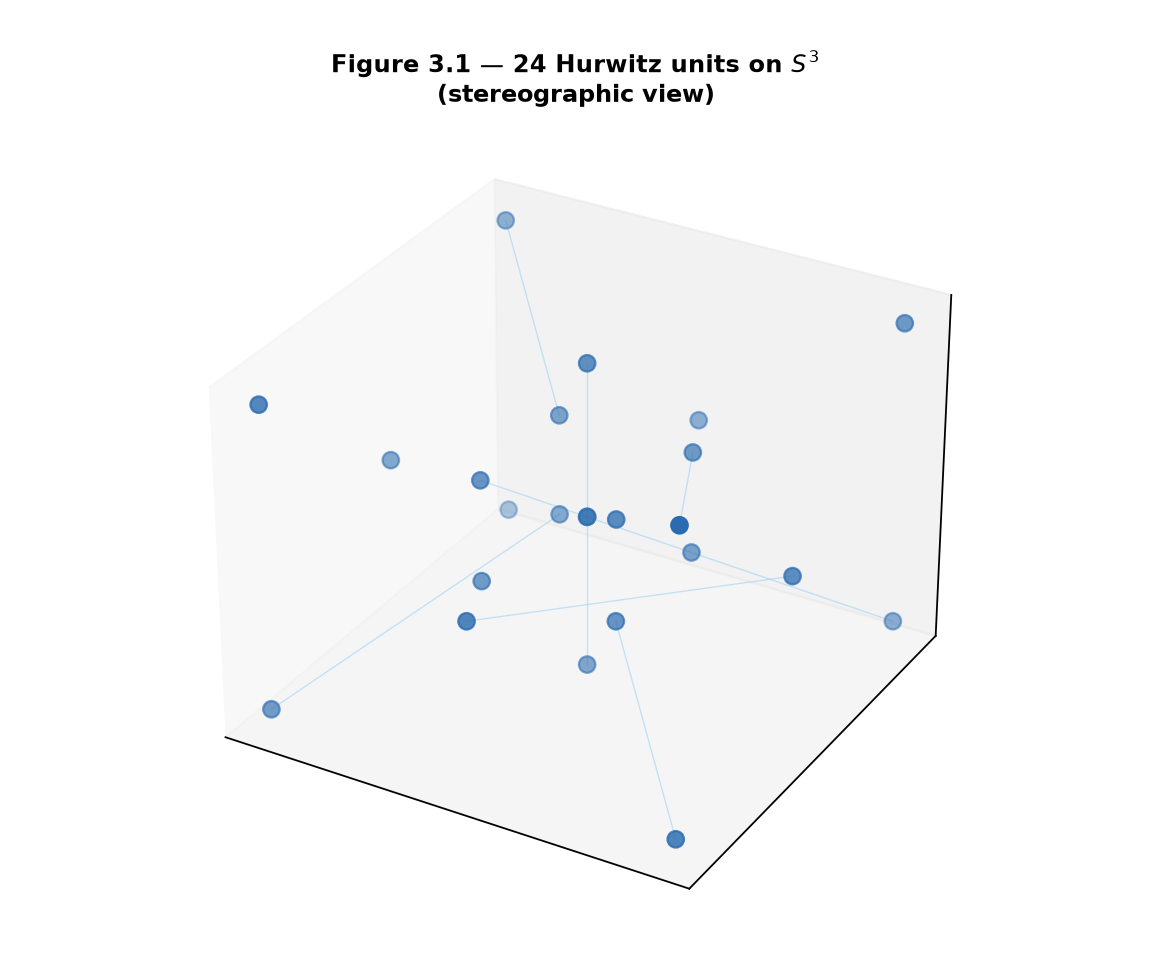
\includegraphics[width=0.92\textwidth,height=0.42\textheight,keepaspectratio]{fig3_1_hurwitz_lattice_in_s3.png}
  \caption{Figure 3.1 --- 24 Hurwitz units on \(S^3\) (stereographic).}
  \label{fig:fig3-1-hurwitz-lattice-in-s3}
\end{figure}

\begin{quote}\small\textit{Figure 3.1.* The 24 Hurwitz units after stereographic projection to \(\mathbb{R}^3\). This is the smallest nontrivial discrete substrate for total-space geometry compatible with Chapter 1.}\end{quote}

\subsection{Density beyond 24 points}
\label{ch:ch03_lattice:density-beyond-24-points}

A theory with only 24 sites is too sparse for Farey-style adjacency, continued-fraction walks, or continuum-like flux. We therefore work with \textbf{nested levels} of discreteness:

\begin{center}
\small
\setlength{\tabcolsep}{4pt}
\begin{tabularx}{\textwidth}{@{}>{\raggedright\arraybackslash}p{0.12\textwidth}>{\raggedright\arraybackslash}X>{\raggedright\arraybackslash}X@{}}
\toprule
Level & Object & Role \\
\midrule
\(\Lambda_0\) & Hurwitz units (\(N=1\)) & Exact arithmetic skeleton; discrete gauge group \\
\(\Lambda_n\) & \(\{q/\lvert q\rvert : q\in\mathcal{H},\; N(q)=n\}\) (optional) & Norm shells; arithmetic depth (Ch. 9) \\
\(\Lambda_{\mathrm{ang}}\) & Samples of Hopf angles \((\eta,\xi_1,\xi_2)\) & Dense visualization / numerical OP1 tests \\
\(\Lambda_{\mathrm{dyn}}\) & Site quaternions in \texttt{TwoGyroLattice} & Dynamical Model used in the portal \\
\bottomrule
\end{tabularx}
\end{center}


\textbf{Software fact.} The book helper \texttt{qga/\allowbreak{}lib/\allowbreak{}hopf\_\allowbreak{}lattice.\allowbreak{}py} implements \(\Lambda_0\) and \(\Lambda_{\mathrm{ang}}\) for labs and figures. Kingdom Come's live portal currently emphasizes \(\Lambda_{\mathrm{dyn}}\) (see ?3.6).

\bigskip
\noindent\rule{\textwidth}{0.4pt}
\bigskip

\section{3.2 The gauged Hopf lattice}
\label{ch:ch03_lattice:3-2-the-gauged-hopf-lattice}

\subsection{Projection via the Hopf map}
\label{ch:ch03_lattice:projection-via-the-hopf-map}

Apply the Hopf map \(h: S^3\to S^2\) (Chapter 2) to a discrete set \(\Lambda\subset S^3\). The image \(h(\Lambda)\) is a discrete set of base points. Each fiber over those base points may contain multiple samples from \(\Lambda\) (phase discretization).

\begin{figure}[htbp]
  \centering
  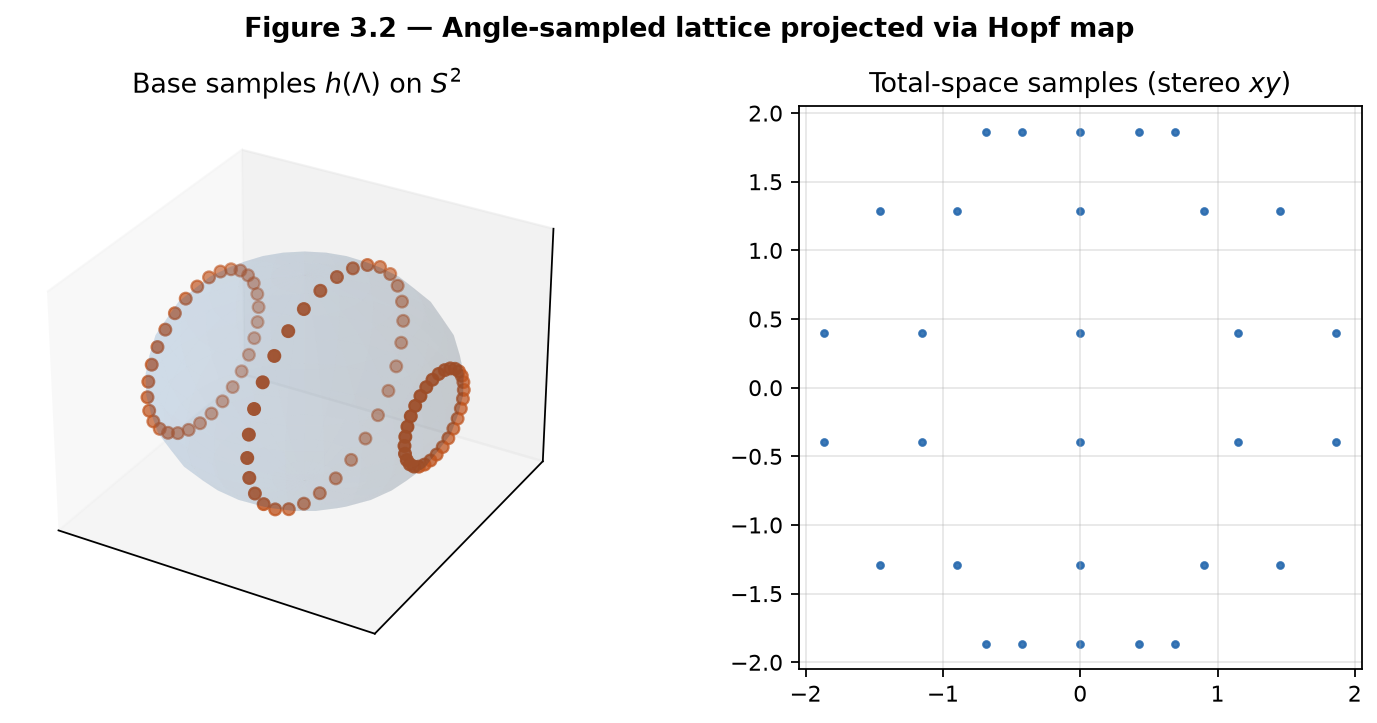
\includegraphics[width=0.92\textwidth,height=0.42\textheight,keepaspectratio]{fig3_2_hopf_projected_lattice.png}
  \caption{Figure 3.2 --- Angle-sampled lattice projected via Hopf.}
  \label{fig:fig3-2-hopf-projected-lattice}
\end{figure}

\begin{quote}\small\textit{Figure 3.2.* Left: base samples on \(S^2\). Right: total-space samples in a stereographic \(xy\) view. Generated from \texttt{sample\_\allowbreak{}angle\_\allowbreak{}lattice} + \texttt{hopf\_\allowbreak{}project\_\allowbreak{}points} in the book helper.}\end{quote}

\subsection{Definition (working)}
\label{ch:ch03_lattice:definition-working}

We define a \textbf{gauged Hopf lattice} as a tuple

\[
\bigl(\Lambda,\; h(\Lambda),\; E_{\parallel},\; E_{\perp},\; \mathcal{G}\bigr)
\]

where:

\begin{itemize}
\item \(\Lambda\subset S^3\) is a discrete point set (one of the levels above),  
\item \(h(\Lambda)\) is its Hopf image on the base,  
\item \(E_{\parallel}\) is the set of \textbf{along-fiber} edges (phase neighbors),  
\item \(E_{\perp}\) is the set of \textbf{inter-fiber} edges (base-neighbor lifts),  
\item \(\mathcal{G}\) is a group of \textbf{gauge transformations} acting on \(\Lambda\) (left/right multiplications by units, and continuous one-parameter subgroups in the dynamical Model).
\end{itemize}

\subsection{Adjacency rules (\textbf{Model} / OP1)}
\label{ch:ch03_lattice:adjacency-rules-model-op1}

Two lattice points \(q_1,q_2\in\Lambda\) may be declared adjacent in either of two ways:

\begin{enumerate}
\item **Along-fiber (\(E_{\parallel}\)).** They lie on (approximately) the same Hopf fiber and are neighbors in discrete phase \(\xi_2\).  
\item **Inter-fiber (\(E_{\perp}\)).** Their base points \(h(q_1),h(q_2)\) are neighbors under a discrete rule on \(S^2\), and a lift to \(S^3\) is chosen (gauge condition).
\end{enumerate}

A \textbf{mediant-like rule} would supply, for adjacent base points, a canonical ``sum'' or interpolant in the total space---exactly the quaternionic lift of Hatcher's

\[
\frac{a}{c}\oplus\frac{b}{d}=\frac{a+b}{c+d}.
\]

No single such rule is yet proved canonical.

\begin{figure}[htbp]
  \centering
  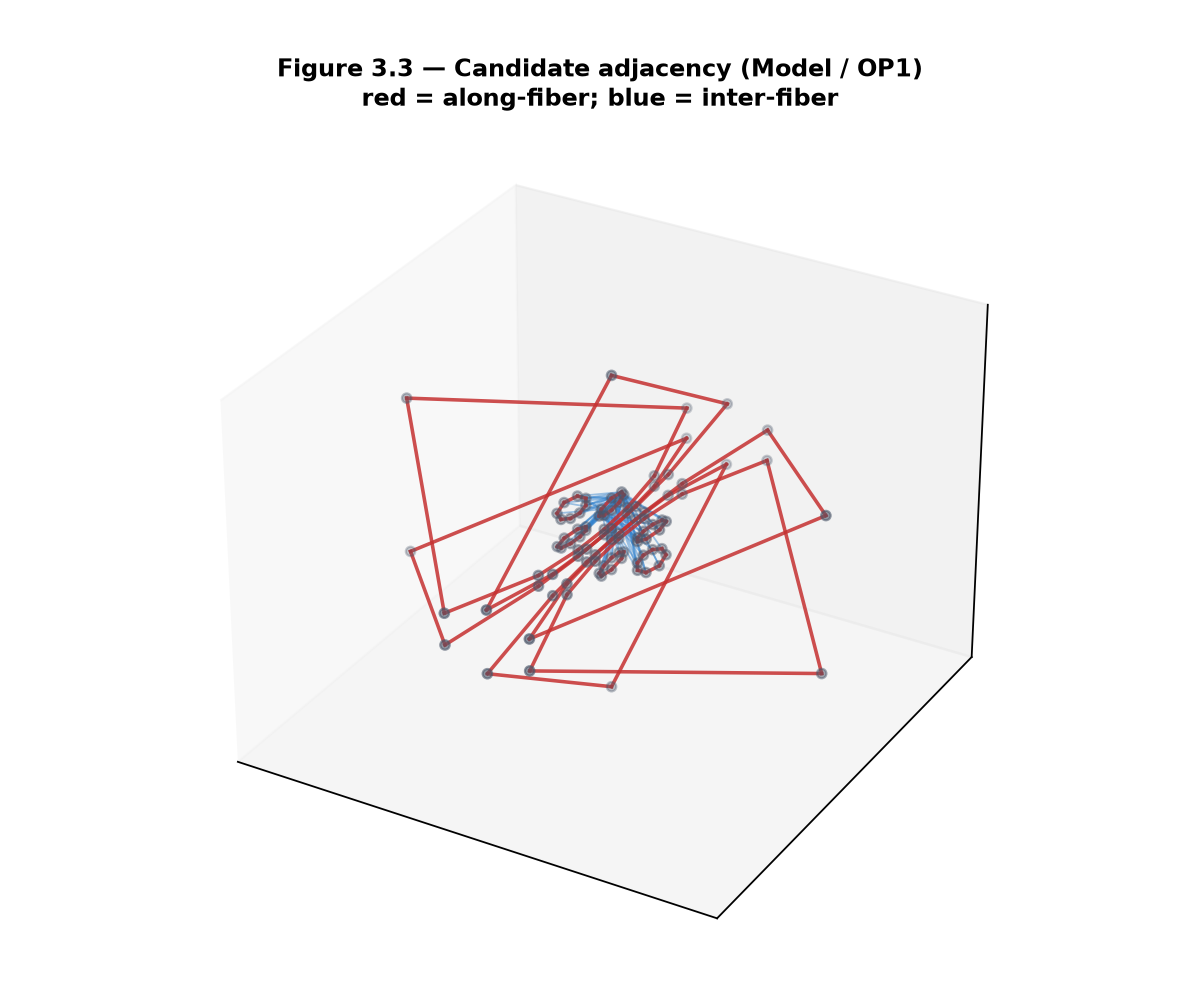
\includegraphics[width=0.92\textwidth,height=0.42\textheight,keepaspectratio]{fig3_3_adjacency_and_fibers.png}
  \caption{Figure 3.3 --- Candidate adjacency (Model / OP1).}
  \label{fig:fig3-3-adjacency-and-fibers}
\end{figure}

\begin{quote}\small\textit{Figure 3.3.* Red: along-fiber edges. Blue: inter-fiber edges from a \textbf{candidate} rule (angular nearest neighbors on the base after Hopf projection, plus phase neighbors). This is an experimental combinatorial object, not a theorem.}\end{quote}

\textbf{Model note.} The adjacency relation is a design choice that \emph{should} reduce to classical Farey adjacency under a suitable projection or restriction. That reduction (and uniqueness among reasonable choices) is \textbf{Open Problem 1}.

\subsection{Candidate rule used in figures and labs}
\label{ch:ch03_lattice:candidate-rule-used-in-figures-and-labs}

The book helper implements one explicit candidate (\texttt{candidate\_\allowbreak{}adjacency}):

\begin{itemize}
\item Recover rough \((\eta,\xi_1,\xi_2)\) from coordinates.  
\item Along-fiber: close in \((\eta,\xi_1)\), neighboring in \(\xi_2\).  
\item Inter-fiber: angular distance on \(S^2\) below a threshold; exclude along-fiber pairs.
\end{itemize}

Other candidates (spherical Delaunay on the base, Hurwitz-norm determinants, geodesic mediants, ...) are welcome; record them against OP1.

\bigskip
\noindent\rule{\textwidth}{0.4pt}
\bigskip

\section{3.3 Gauge actions: left and right multiplications}
\label{ch:ch03_lattice:3-3-gauge-actions-left-and-right-multiplications}

From Chapters 1--2:

\begin{itemize}
\item \textbf{Left multiplication} \(q\mapsto uq\) (unit \(u\)) is an isometry of \(S^3\), maps fibers to fibers, and induces a rotation of the base \(S^2\).  
\item \textbf{Right multiplication} \(q\mapsto qu\) is an isometry; in the classical complex picture it implements fiberwise \(U(1)\) phase (structure-group action).
\end{itemize}

On a discrete set \(\Lambda\) we therefore equip two families of \textbf{gauge transformations}:

\begin{center}
\small
\setlength{\tabcolsep}{4pt}
\begin{tabularx}{\textwidth}{@{}>{\raggedright\arraybackslash}p{0.12\textwidth}>{\raggedright\arraybackslash}X>{\raggedright\arraybackslash}X@{}}
\toprule
Action & Continuous & Discrete (Hurwitz) \\
\midrule
Left & \(u\in S^3\) & \(u\in\Lambda_0\) (24 units) \\
Right & \(u\in S^3\) (esp. fiber \(U(1)\)) & \(u\in\Lambda_0\) \\
\bottomrule
\end{tabularx}
\end{center}


When \(\Lambda=\Lambda_0\), left/right multiplications by units \textbf{permute} the lattice exactly. On denser samples they move points within \(S^3\); one may re-snap to nearest lattice points (another OP1 design choice).

\begin{figure}[htbp]
  \centering
  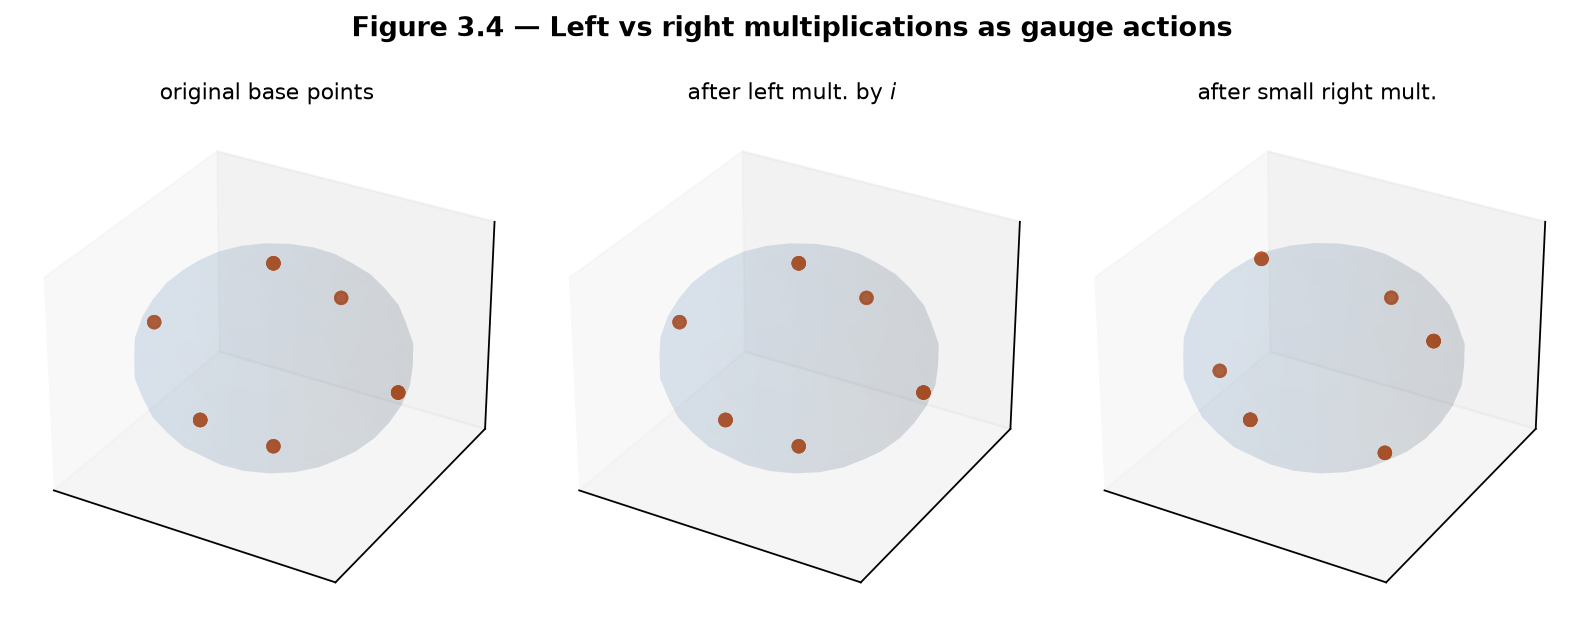
\includegraphics[width=0.92\textwidth,height=0.42\textheight,keepaspectratio]{fig3_4_gauge_action.png}
  \caption{Figure 3.4 --- Left vs right multiplications as gauge actions.}
  \label{fig:fig3-4-gauge-action}
\end{figure}

\begin{quote}\small\textit{Figure 3.4.* Hopf images of the 24 Hurwitz units: original; after left multiplication by \(i\); after a small right multiplication (phase-like). Left multiplication by a Hurwitz unit \textbf{permutes} \(\Lambda_0\), so the multiset of base points is invariant even though individual assignments change (see Lab 3.C note and Ch. 4 Lab 4.A).}\end{quote}

\subsection{Dynamical gauge in the portal (\textbf{Model} + software)}
\label{ch:ch03_lattice:dynamical-gauge-in-the-portal-model-software}

Kingdom Come's \texttt{TwoGyroLattice} does not store a static Farey graph. It evolves \(n\) site quaternions with left/right rotors and a global \textbf{gauge rotation} driven by mean twist imbalance:

\[
q_i \;\leftarrow\; \delta_L\, q_i\, \overline{\delta_R},
\quad\text{then}\quad
q_i \;\leftarrow\; q_i\, g(\alpha),
\]

with gauge angle \(\alpha\) proportional to average twist. \textbf{Identity preservation} tracks how well a parallel-transported identity field stays aligned---stable vs chaotic modes differ mainly in \texttt{gauge\_\allowbreak{}strength} and detuning. This is a \textbf{dynamical Model} of gauged flux, not yet a combinatorial Farey theory.

\bigskip
\noindent\rule{\textwidth}{0.4pt}
\bigskip

\section{3.4 Flux configurations and flywheels (first introduction)}
\label{ch:ch03_lattice:3-4-flux-configurations-and-flywheels-first-introduction}

\subsection{Discrete flux}
\label{ch:ch03_lattice:discrete-flux}

A \textbf{flux configuration} on the gauged Hopf lattice is an assignment of oriented edge weights

\[
\Phi: E_{\parallel}\cup E_{\perp} \to \mathbb{Z}
\]

(or to \(\mathbb{R}\), in continuum limits) that transforms naturally under gauge actions and satisfies a discrete conservation law at vertices (coboundary / Kirchhoff condition)---to be refined in Chapter 5 with topographs.

\subsection{Flux flywheel}
\label{ch:ch03_lattice:flux-flywheel}

A \textbf{flux flywheel} is a closed, topologically protected circulating flux configuration: a periodic orbit of gauge and phase that cannot unwind continuously without cutting a linked fiber or violating gauge constraints. In the continuous / dynamical limit these become the rotating flux structures of the Kingdom Come Model (Ch. 0, Fig. 0.4; portal Flux Flywheel tab).

\begin{figure}[htbp]
  \centering
  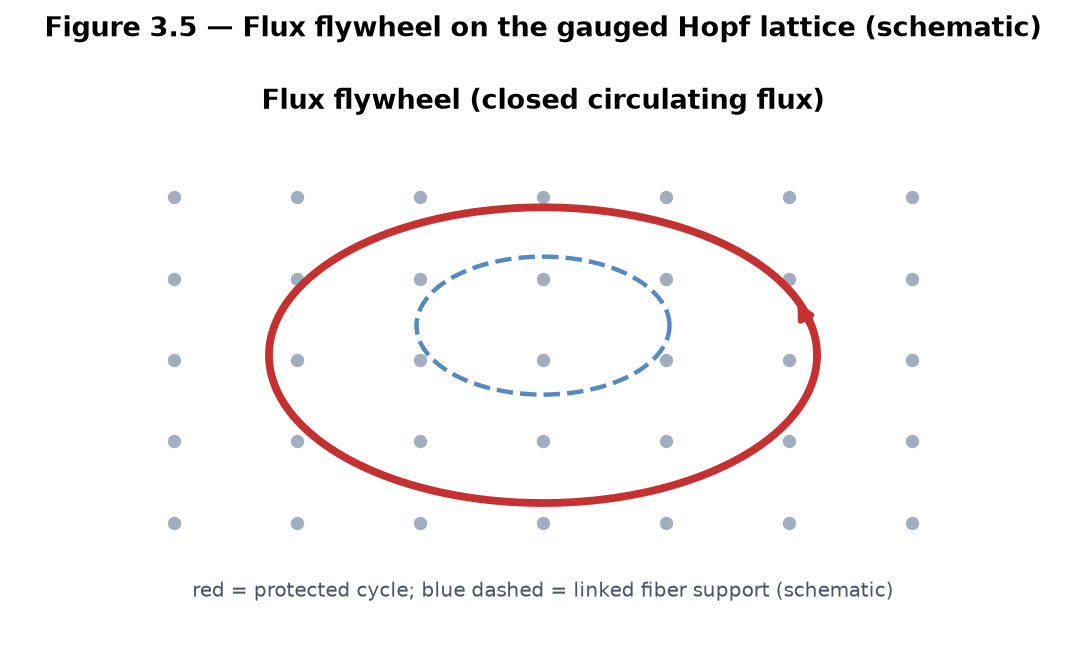
\includegraphics[width=0.92\textwidth,height=0.42\textheight,keepaspectratio]{fig3_5_flux_flywheel_schematic.png}
  \caption{Figure 3.5 --- Flux flywheel schematic.}
  \label{fig:fig3-5-flux-flywheel-schematic}
\end{figure}

\begin{quote}\small\textit{Figure 3.5.* Closed circulating flux (red) supported on lattice edges and fibers; a linked fiber (blue dashed) hints at the topological obstruction to trivialization.}\end{quote}

\textbf{Claim type.} Existence and stability of flywheels as \emph{physical} objects: \textbf{Model}. Linking of Hopf fibers as a classical topological fact: \textbf{Theorem} (Ch. 2). Mapping flywheels to atomic number \(Z\): later chapters (\textbf{Model} / \textbf{Hypothesis}).

\bigskip
\noindent\rule{\textwidth}{0.4pt}
\bigskip

\section{3.5 Open Problem 1 --- Canonical quaternionic Farey structure}
\label{ch:ch03_lattice:3-5-open-problem-1-canonical-quaternionic-farey-structure}

\textbf{Open Problem 1 (core of this chapter and of Part II).} Prove uniqueness (or classify all reasonable choices) of discrete adjacency / mediant rules on the gauged Hopf lattice such that:

\begin{enumerate}
\item The structure \textbf{reduces to the classical Farey diagram} under a suitable projection or restriction (e.g. a fixed complex line, a parabolic subgroup, or a 2D slice of base coordinates).  
\item Adjacency is \textbf{compatible} with left and right gauge actions (equivariance).  
\item The resulting graph admits a natural notion of \textbf{continued-fraction paths} (discrete walks that refine approximants), including walks that advance primarily \textbf{along fibers}.  
\item (Optional but desirable.) A Euclidean or greedy algorithm on the lattice recovers shortest paths analogous to Farey mediants.
\end{enumerate}

\textbf{Current status (draft).}

\begin{center}
\small
\setlength{\tabcolsep}{4pt}
\begin{tabularx}{\textwidth}{@{}>{\raggedright\arraybackslash}X>{\raggedright\arraybackslash}X@{}}
\toprule
Layer & Status \\
\midrule
Hurwitz units \(\Lambda_0\) & Classical, settled \\
Hopf projection of discrete sets & Implemented (portal + book helper) \\
Candidate adjacency (\texttt{candidate\_\allowbreak{}adjacency}) & Numerical experiments only --- \textbf{not} proved canonical \\
Reduction to Farey \(\lvert ad-bc\rvert=1\) & \textbf{Open} \\
Equivariant mediant & \textbf{Open} \\
Dynamical two-gyro lattice & Portal demo; parallel track to combinatorial theory \\
\bottomrule
\end{tabularx}
\end{center}


\textbf{Research target.} Any reader who solves or substantially advances Open Problem 1 produces the central combinatorial object of the entire book.

See also \texttt{notes/\allowbreak{}open\_\allowbreak{}problems.\allowbreak{}md} (OP1 status tracking).

\bigskip
\noindent\rule{\textwidth}{0.4pt}
\bigskip

\section{3.6 Software map and first computational labs}
\label{ch:ch03_lattice:3-6-software-map-and-first-computational-labs}

\begin{center}
\small
\setlength{\tabcolsep}{4pt}
\begin{tabularx}{\textwidth}{@{}>{\raggedright\arraybackslash}X>{\raggedright\arraybackslash}X@{}}
\toprule
Component & Location \\
\midrule
\texttt{LatticeConfig} & \texttt{kingdom.\allowbreak{}core.\allowbreak{}lattice} \\
\texttt{TwoGyroLattice} & \texttt{kingdom.\allowbreak{}simulations.\allowbreak{}lattice} \\
Hurwitz / adjacency / gauge & \texttt{lib/\allowbreak{}hopf\_\allowbreak{}lattice.\allowbreak{}py} \\
\bottomrule
\end{tabularx}
\end{center}


\textbf{Honest gap.} No production \texttt{build\_\allowbreak{}hurwitz\_\allowbreak{}lattice\_\allowbreak{}sample} in Kingdom Come yet --- pedagogy lives in \texttt{lib/\allowbreak{}}.

\textbf{Labs (short form).} Full code: \textbf{Appendix C ?C.2}.

\begin{itemize}
\item \textbf{3.A} 24 Hurwitz units; Hopf project; count base points.
\item \textbf{3.B} \texttt{sample\_\allowbreak{}angle\_\allowbreak{}lattice} + \texttt{candidate\_\allowbreak{}adjacency} (OP1 sandbox).
\item \textbf{3.C} Left \(	imes i\): base \textbf{set} invariant, total-space points move (see Lab 4.A).
\item \textbf{3.D} \texttt{run\_\allowbreak{}lattice\_\allowbreak{}comparison} stable vs chaotic.
\item \textbf{3.E} Toy \texttt{discrete\_\allowbreak{}flux\_\allowbreak{}cycle}.
\end{itemize}

\begin{lstlisting}[style=qga,language=python]
from lib.hopf_lattice import HURWITZ_UNITS, hopf_project_points
print(len(HURWITZ_UNITS), hopf_project_points(HURWITZ_UNITS).shape)
\end{lstlisting}

\bigskip
\noindent\rule{\textwidth}{0.4pt}
\bigskip

\section{Exercises}
\label{ch:ch03_lattice:exercises}

\textbf{3.A (hand).} List the 24 Hurwitz units and verify \(N(q)=1\) for each family (\(\pm 1,\pm i,\pm j,\pm k\) and half-integer units).

\textbf{3.B (hand).} In two sentences, describe how left multiplication by a fixed unit quaternion acts on the base \(S^2\) via the Hopf map.

\textbf{3.C (code).} Complete Labs 3.A--3.C. Report the number of approximate distinct base points for \(\Lambda_0\) and for one angle lattice. For Lab 3.C, confirm that the sorted base multiset is invariant under left multiplication by \(i\) while some index-wise base coordinates still move.

\textbf{3.D (code).} Apply a sequence of small right multiplications to \(\Lambda_0\) (or one fiber of \(\Lambda_{\mathrm{ang}}\)) and check approximate return after total angle \(2\pi\).

\textbf{3.E (visual / dynamical).} Run Lab 3.D (simulator) or the Gradio Lattice Simulator. Describe what ``identity preservation'' looks like for stable vs chaotic modes.

\textbf{3.F (Hatcher bridge).} In Hatcher, two fractions \(a/c\) and \(b/d\) are Farey-adjacent iff \(\lvert ad-bc\rvert=1\). Propose a quaternionic analogue (e.g. \(\lvert N(q_1\overline{q_2}-q_2\overline{q_1})\rvert\) or a \(2\times 2\) minor from complex pairs) and test it numerically on \(\Lambda_0\) or \(\Lambda_{\mathrm{ang}}\). Record whether it recovers a subgraph of \texttt{candidate\_\allowbreak{}adjacency}.

\textbf{3.G (forward).} Why is topological linking of fibers a natural candidate for the protection mechanism of flux flywheels? (Developed in Chapters 5 and 10.)

\textbf{3.H (Open Problem 1 teaser).} Run the current \texttt{candidate\_\allowbreak{}adjacency} implementation. Does it reduce to classical Farey adjacency under any obvious projection or 2D slice? Document one negative or partial observation---progress often starts as a failed reduction.

\textbf{3.I (software honesty).} In one paragraph, distinguish: (i) Hurwitz arithmetic lattice, (ii) angle-sampled visualization lattice, (iii) two-gyro dynamical lattice. Which claim types apply to each?

\bigskip
\noindent\rule{\textwidth}{0.4pt}
\bigskip

\section{Code and asset pointers}
\label{ch:ch03_lattice:code-and-asset-pointers}

\begin{lstlisting}[style=qga]
# Book pedagogy (this repo)
qga/lib/hopf_lattice.py
  HURWITZ_UNITS, sample_angle_lattice, hopf_project_points,
  candidate_adjacency, left_multiply, right_multiply, discrete_flux_cycle

# Kingdom Come
kingdom.core.lattice.LatticeConfig
kingdom.simulations.lattice.TwoGyroLattice
kingdom.simulations.lattice.run_lattice_comparison
kingdom.simulations.lattice.build_lattice_figure
kingdom.core.hopf                    # projection / fibers
\end{lstlisting}

\textbf{Figures:} \texttt{scripts/\allowbreak{}generate\_\allowbreak{}ch3\_\allowbreak{}figures.\allowbreak{}py} \textbf{Related portal:} Lattice Simulator tab --- dynamical counterpart of Aux A3.1. \textbf{Open problems:} \texttt{notes/\allowbreak{}open\_\allowbreak{}problems.\allowbreak{}md} \(\cdot\) OP1.

\bigskip
\noindent\rule{\textwidth}{0.4pt}
\bigskip

\section{Looking ahead}
\label{ch:ch03_lattice:looking-ahead}

We now possess the discrete geometric object at the heart of the book: the \textbf{gauged Hopf lattice}, still with a \textbf{Model}-level adjacency rule pending OP1. In \textbf{Chapter 4} we study its symmetries in detail---the full gauge group generated by left and right actions, periodicity, and comparison with Hatcher's linear fractional transformations. Chapters 5--7 develop flux topographs, classification, and the \(Z\mapsto\) flywheel map on this lattice.

\textbf{Forward pointer (invariant discipline).} The lattice of this chapter is already a place where discrete combinatorial structure meets continuous \(S^3\) geometry. Later chapters will assign \textbf{labels}, \textbf{scores}, and \textbf{classes} to configurations. When that happens, keep the discipline developed fully in \textbf{Chapter 9, section 9.5}: algebraic cycle structure, sequential label progression, and true angle--label lock are \emph{different} invariants. Visual order is not statistical locking unless tested against a null. Full treatment, figure, and controls: Chapter 9 section 9.5 \(\cdot\) \texttt{notes/\allowbreak{}RESEARCH\_\allowbreak{}NOTE\_\allowbreak{}moduli.\allowbreak{}md} \(\cdot\) supporting stack \texttt{vortex\_\allowbreak{}math}.

With the gauged Hopf lattice constructed, we are ready to examine its symmetries---the higher-dimensional lift of the linear fractional transformations that organize Hatcher's Farey diagram.

\bigskip
\noindent\rule{\textwidth}{0.4pt}
\bigskip



% Auto-generated from book/04_symmetries.md — do not edit by hand
% Regenerated by scripts/md_to_latex.py

\chapter{Chapter 4 --- Symmetries of the Gauged Hopf Lattice}
\label{ch:ch04_symmetries}

This chapter examines the symmetries generated by left and right multiplications on the gauged Hopf lattice of Chapter 3. These actions play the role that linear fractional transformations play for Hatcher's Farey diagram. We classify periodic structures, glide-like motions, and rotational symmetries, and see how the gauge group acts on flux configurations and flywheels.

\textbf{Learning goals}

\begin{enumerate}
\item Treat left and right multiplications as the fundamental gauge symmetries of the lattice.  
\item Compare the quaternionic gauge actions with Hatcher's linear fractional transformations.  
\item Identify periodic orbits, glide-like actions, and rotational symmetries.  
\item Understand how symmetries act on flux configurations and preserve (or map) flywheels.  
\item Prepare the symmetry language required for flux topographs (Chapter 5).
\end{enumerate}

\textbf{Figures in this chapter}

\begin{center}
\small
\begin{tabular}{@{}lp{0.28\textwidth}p{0.28\textwidth}@{}}
\toprule
Tag & File & Role \\
\midrule
Fig. 4.1 & \texttt{figures/fig4\_1\_left\_right\_symmetries.png} & Left vs right gauge actions on base and fibers \\
Fig. 4.2 & \texttt{figures/fig4\_2\_periodic\_orbit.png} & Orbit under combined gauge sequence \\
Fig. 4.3 & \texttt{figures/fig4\_3\_glide\_reflection\_analogue.png} & Glide-like helical symmetry \\
Fig. 4.4 & \texttt{figures/fig4\_4\_symmetry\_on\_flywheel.png} & Gauge symmetry preserving a flux flywheel \\
Aux A4.1 & \texttt{figures/aux4\_1\_gauge\_group\_elements.png} & Discrete gauge elements (24 Hurwitz units) \\
\bottomrule
\end{tabular}
\end{center}


\textbf{Claim discipline}

\begin{center}
\small
\begin{tabular}{@{}lp{0.55\textwidth}@{}}
\toprule
Claim & Type \\
\midrule
Left and right multiplications are isometries of \(S^3\); classical Hopf bundle structure group & \textbf{Theorem} \\
Discrete gauge actions as ``the modular group of the lattice''; equivariance of candidate adjacency; glide analogues & \textbf{Model} (pending OP1) \\
Action of gauge on flux/flywheels in the combinatorial and dynamical Models & \textbf{Model} \\
\texttt{qga/lib/hopf\_lattice.py} symmetry helpers; \texttt{TwoGyroLattice} gauge evolution & \textbf{Software fact} \\
\bottomrule
\end{tabular}
\end{center}


\bigskip
\noindent\rule{\textwidth}{0.4pt}
\bigskip

\section{4.1 Left and right multiplications as gauge symmetries}
\label{ch:ch04_symmetries:4-1-left-and-right-multiplications-as-gauge-symmetries}

Chapter 3 equipped the gauged Hopf lattice with two families of gauge transformations coming directly from quaternion multiplication:

\begin{itemize}
\item \textbf{Left multiplication} \(q \mapsto u q\) (fixed unit \(u\)) is an isometry of \(S^3\). It maps fibers to fibers and induces a rotation of the base \(S^2\) via the Hopf map.  
\item \textbf{Right multiplication} \(q \mapsto q u\) is an isometry; in the classical complex picture it implements the fiberwise \(U(1)\) phase (the structure-group action of the bundle).
\end{itemize}

On a discrete set \(\Lambda\) these become the operational gauge symmetries.

\begin{center}
\small
\begin{tabular}{@{}lp{0.28\textwidth}p{0.28\textwidth}@{}}
\toprule
Domain & Left action & Right action \\
\midrule
\(\Lambda_0\) (24 Hurwitz units) & Permutes \(\Lambda_0\) exactly & Permutes \(\Lambda_0\) exactly \\
\(\Lambda_{\mathrm{ang}}\) (angle sample) & Moves samples in \(S^3\) & Moves samples (phase-like) \\
\(\Lambda_{\mathrm{dyn}}\) (\texttt{TwoGyroLattice}) & Continuous rotors \(\delta_L\) & Continuous rotors \(\delta_R\) + global gauge \(g(\alpha)\) \\
\bottomrule
\end{tabular}
\end{center}


Re-snapping a moved dense sample to a nearest lattice point is a design choice tied to \textbf{Open Problem 1} (canonical adjacency must decide how continuous symmetries interact with discrete graphs).

\begin{figure}[htbp]
  \centering
  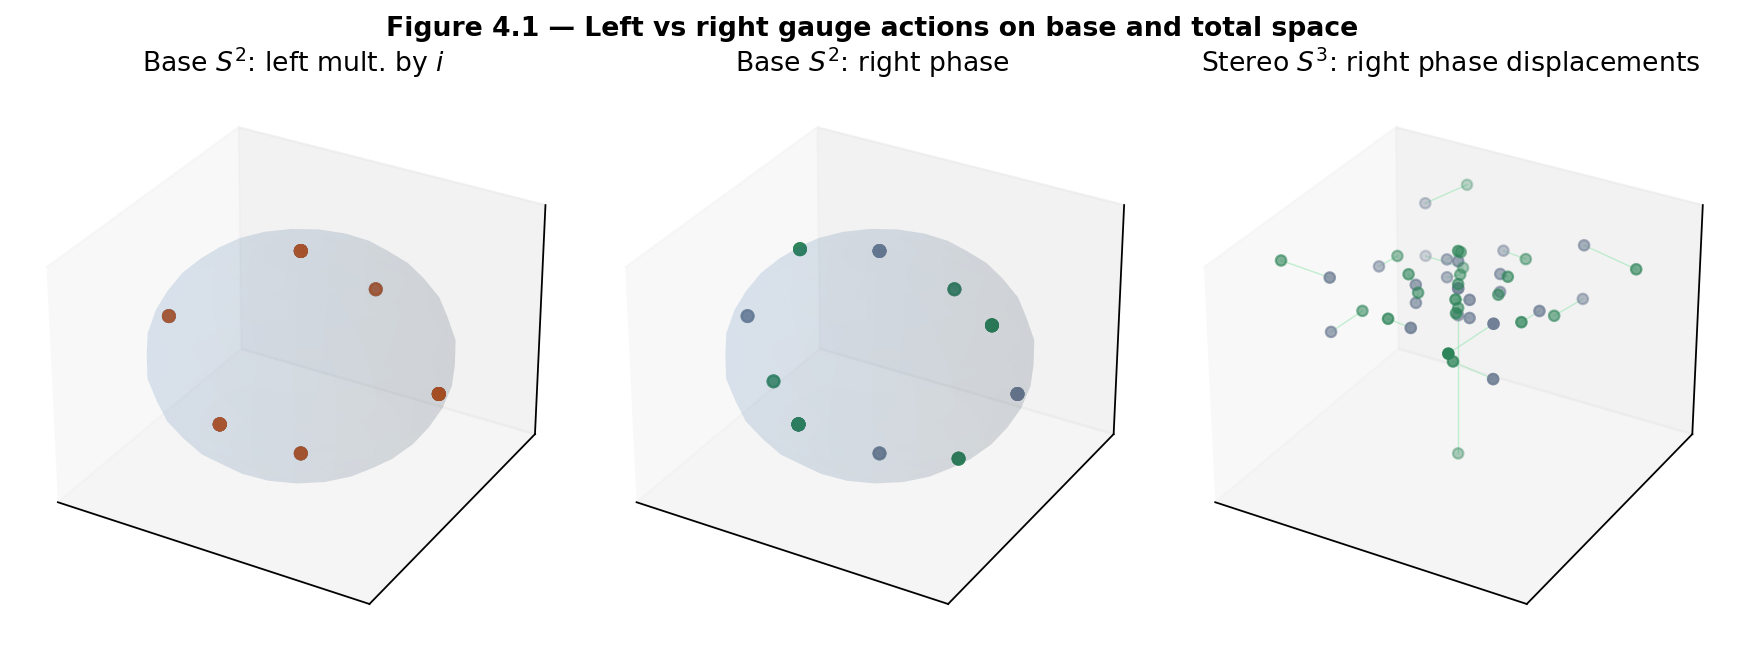
\includegraphics[width=0.92\textwidth,height=0.42\textheight,keepaspectratio]{fig4_1_left_right_symmetries.png}
  \caption{Figure 4.1 --- Left versus right gauge actions.}
  \label{fig:fig4-1-left-right-symmetries}
\end{figure}

\begin{quote}\small\textit{Figure 4.1.* Left: base points of the Hurwitz units under left multiplication by \(i\). Middle: base under a small right phase. Right: stereographic displacements under the same right phase. Because left multiplication by a Hurwitz unit \textbf{permutes} \(\Lambda_0\), the multiset of projected base points is invariant---individual assignments change, but the sorted base set does not.}\end{quote}

\begin{figure}[htbp]
  \centering
  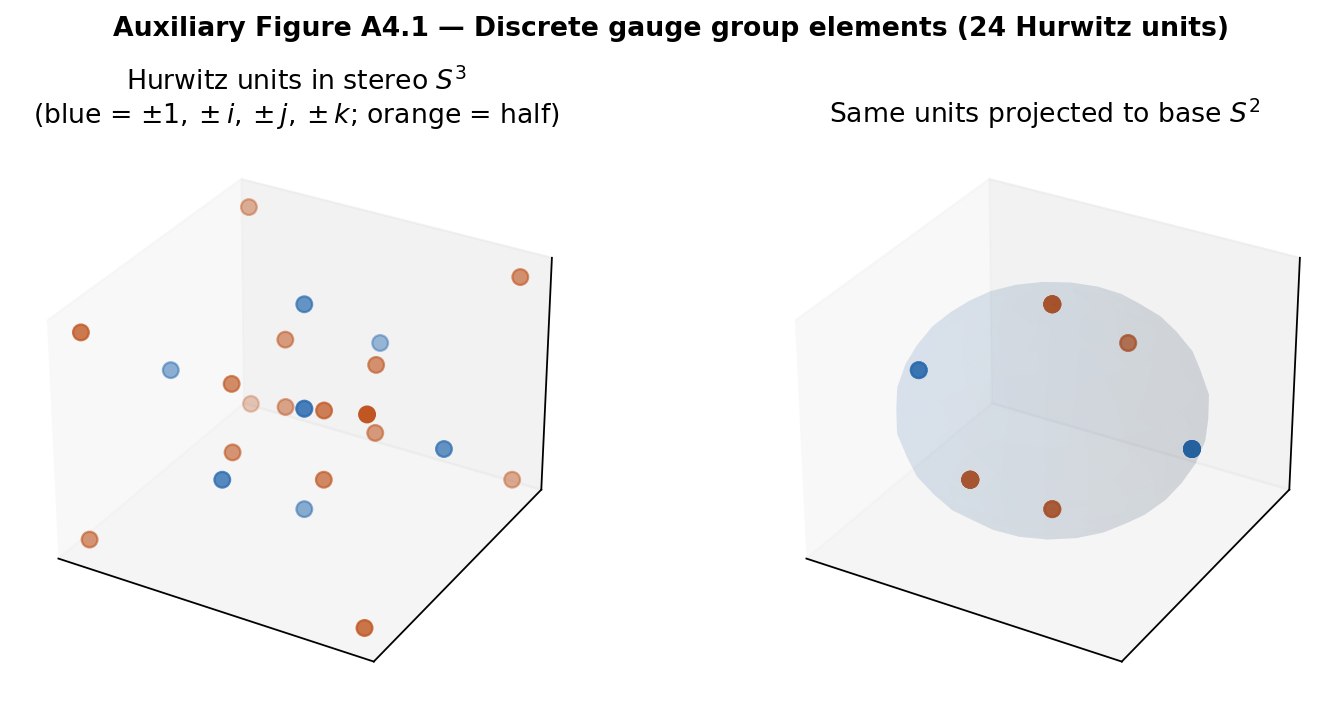
\includegraphics[width=0.92\textwidth,height=0.42\textheight,keepaspectratio]{aux4_1_gauge_group_elements.png}
  \caption{Auxiliary Figure A4.1 --- Discrete gauge group elements.}
  \label{fig:aux4-1-gauge-group-elements}
\end{figure}

\begin{quote}\small\textit{Auxiliary Figure A4.1.* The 24 Hurwitz units as the discrete gauge group generators/elements: stereographic \(S^3\) and Hopf projection to \(S^2\).}\end{quote}

\textbf{Theorem.} For any unit \(u\in S^3\), the maps \(q\mapsto uq\) and \(q\mapsto qu\) are isometries of \(S^3\) with respect to the round metric (they preserve the Euclidean norm on \(\mathbb{R}^4\) and fix the sphere).

\bigskip
\noindent\rule{\textwidth}{0.4pt}
\bigskip

\section{4.2 Comparison with Hatcher's linear fractional transformations}
\label{ch:ch04_symmetries:4-2-comparison-with-hatcher-s-linear-fractional-transformati}

Hatcher organizes the Farey diagram with the action of linear fractional transformations

\[
T(z) = \frac{az+b}{cz+d}, \qquad ad-bc=\pm 1.
\]

These preserve adjacency, generate translations, glide reflections, and rotations, and produce the periodic structures of continued fractions and topographs.

In the gauged Hopf lattice the analogous organizing actions are \textbf{left and right quaternion multiplications}. The structural parallel is strong but remains a \textbf{Model} until a canonical adjacency rule is established (Open Problem 1) and equivariance is proved.

\begin{center}
\small
\begin{tabular}{@{}lp{0.55\textwidth}@{}}
\toprule
Feature in Hatcher & Quaternionic analogue \\
\midrule
Linear fractional transformations (\(\mathrm{PSL}(2,\mathbb{Z})\)) & Left + right multiplications by units \\
Preservation of Farey adjacency & Preservation of candidate adjacency (\textbf{Model} / OP1 test) \\
Translations along periodic strips & Repeated right phase advance along fibers \\
Glide reflections & Combined left+right actions producing helical orbits \\
Rotations about vertices or triangle centers & Left actions that fix or cycle base points \\
Periodic continued-fraction expansions & Periodic orbits under combined gauge sequences \\
\bottomrule
\end{tabular}
\end{center}


The quaternionic version is richer---two interacting actions rather than a single matrix group---and lives on the three-sphere rather than the hyperbolic plane.

\textbf{Claim type.} The parallel is a \textbf{Model} metaphor until OP1 is resolved and an equivariant reduction to the classical Farey case is proved.

\bigskip
\noindent\rule{\textwidth}{0.4pt}
\bigskip

\section{4.3 Periodic orbits and glide-like symmetries}
\label{ch:ch04_symmetries:4-3-periodic-orbits-and-glide-like-symmetries}

\subsection{Periodic orbits}
\label{ch:ch04_symmetries:periodic-orbits}

A finite sequence of left and right multiplications often produces a \textbf{periodic orbit} on the lattice: after \(k\) applications of a composite map \(g\), a point returns (exactly, for \(\Lambda_0\); approximately, for dense samples). These orbits are discrete analogues of the periodic separator lines that appear in Hatcher's topographs and of the closed continued-fraction periods that generate Pell solutions.

\begin{figure}[htbp]
  \centering
  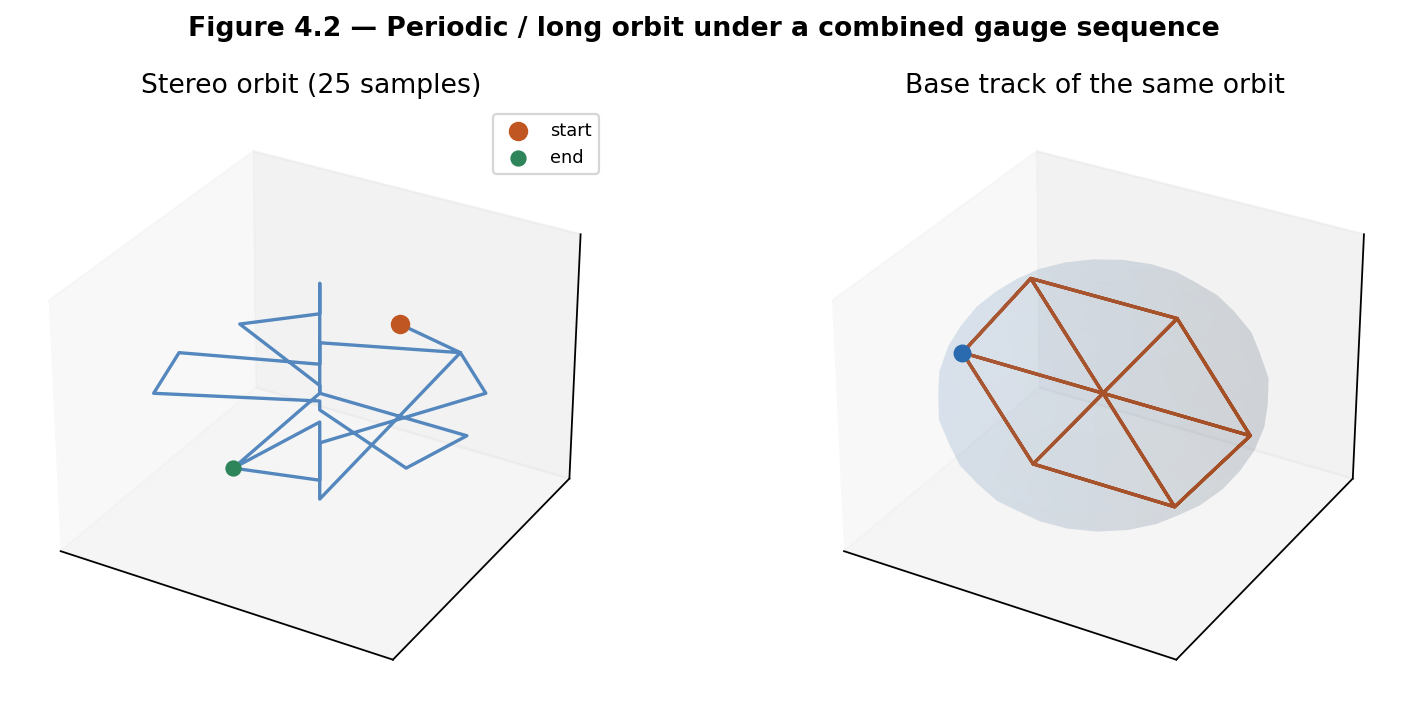
\includegraphics[width=0.92\textwidth,height=0.42\textheight,keepaspectratio]{fig4_2_periodic_orbit.png}
  \caption{Figure 4.2 --- Orbit under a combined gauge sequence.}
  \label{fig:fig4-2-periodic-orbit}
\end{figure}

\begin{quote}\small\textit{Figure 4.2.* Total-space (stereographic) and base tracks of a point under iterated left and right steps. Exact period depends on the sequence; on \(\Lambda_0\) periods divide the order of the induced permutation.}\end{quote}

\subsection{Glide-like symmetries}
\label{ch:ch04_symmetries:glide-like-symmetries}

\textbf{Glide-like symmetries} arise when a right multiplication (phase advance along a fiber) is paired with a left multiplication that shifts the base point. The resulting motion is helical---a higher-dimensional lift of a classical glide reflection along a Farey strip.

\begin{figure}[htbp]
  \centering
  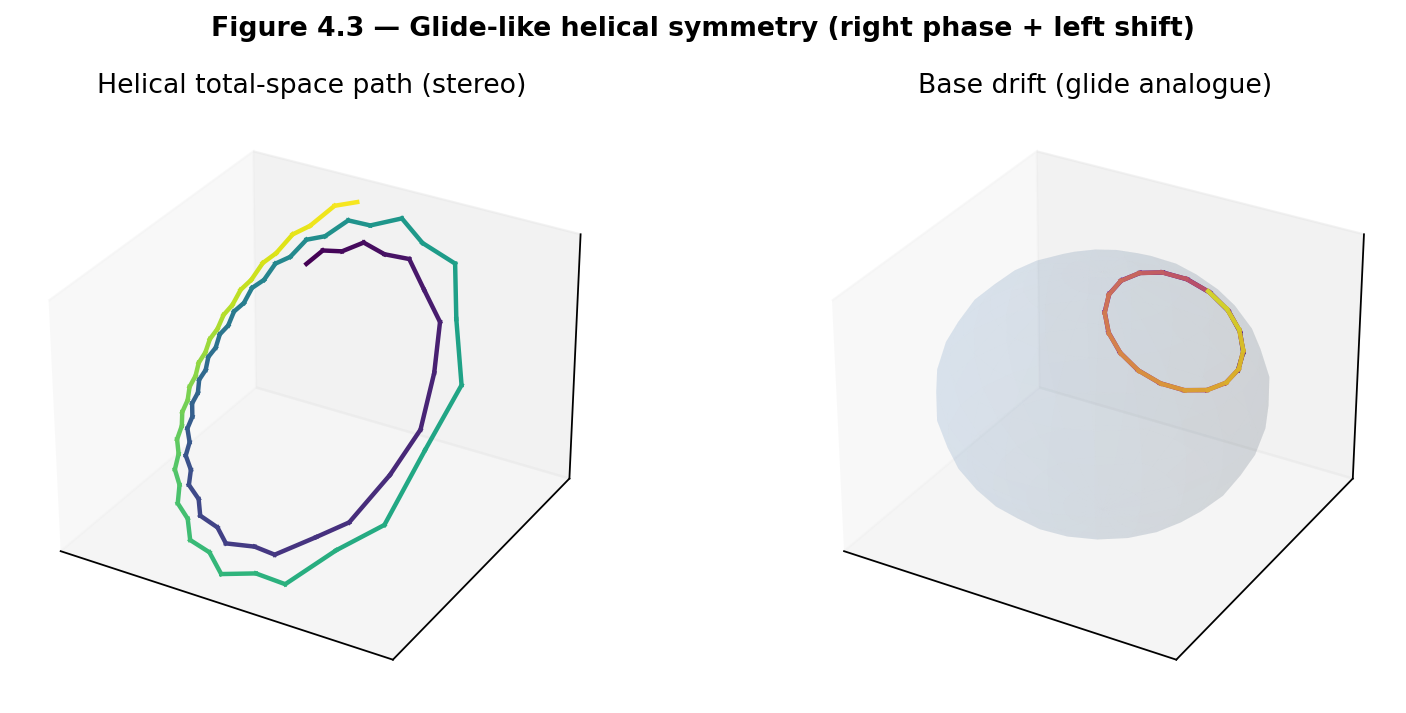
\includegraphics[width=0.92\textwidth,height=0.42\textheight,keepaspectratio]{fig4_3_glide_reflection_analogue.png}
  \caption{Figure 4.3 --- Glide-like helical symmetry.}
  \label{fig:fig4-3-glide-reflection-analogue}
\end{figure}

\begin{quote}\small\textit{Figure 4.3.* Combined right phase + left shift iterated: a helical path in the total space and a drifting track on the base. \textbf{Model} analogue of Hatcher's glide reflections, not a theorem of uniqueness.}\end{quote}

\subsection{Book API for sequences}
\label{ch:ch04_symmetries:book-api-for-sequences}

\begin{lstlisting}[style=qga]
phase_unit(theta)                 # right-phase unit quaternion
apply_gauge_step(points, 'L'|'R', unit)
apply_gauge_sequence(points, [('L', u), ('R', v), ...])
orbit_of_point(q, sequence, max_periods=..., tol=...)
permutes_hurwitz_units(unit, side='L'|'R')
adjacency_equivariance_score(points, unit, side=...)  # OP1 diagnostic
\end{lstlisting}

\bigskip
\noindent\rule{\textwidth}{0.4pt}
\bigskip

\section{4.4 Symmetries acting on flux configurations and flywheels}
\label{ch:ch04_symmetries:4-4-symmetries-acting-on-flux-configurations-and-flywheels}

\subsection{Push-forward of discrete flux}
\label{ch:ch04_symmetries:push-forward-of-discrete-flux}

If \(\Phi: E\to\mathbb{Z}\) assigns oriented flux to edges of the lattice graph, a gauge symmetry \(g\) that maps vertices (and therefore edges) induces

\[
(g\cdot\Phi)(g(e)) = \Phi(e).
\]

Conservation at vertices (discrete \(\mathrm{d}^*\Phi=0\)) is preserved whenever \(g\) is a graph automorphism. When \(g\) only approximately preserves candidate adjacency (OP1 unfinished), flux push-forward is well-defined on the abstract edge set of \(\Lambda\) with indices, but may leave the ``along-fiber / inter-fiber'' typing.

Helpers: \texttt{discrete\_flux\_cycle}, \texttt{transform\_flux}, \texttt{nearest\_index\_map} in \texttt{qga/lib/hopf\_lattice.py}.

\subsection{Flywheels as equivariant cycles}
\label{ch:ch04_symmetries:flywheels-as-equivariant-cycles}

Topologically protected \textbf{flux flywheels} (Ch. 3) are closed circulating configurations whose supporting cycles are mapped to equivalent cycles by the gauge group. The linking of Hopf fibers (Ch. 2, \textbf{Theorem}) supplies a topological obstruction to trivialization that is preserved by all continuous isometries of the fibration---and therefore by left/right multiplications.

\begin{figure}[htbp]
  \centering
  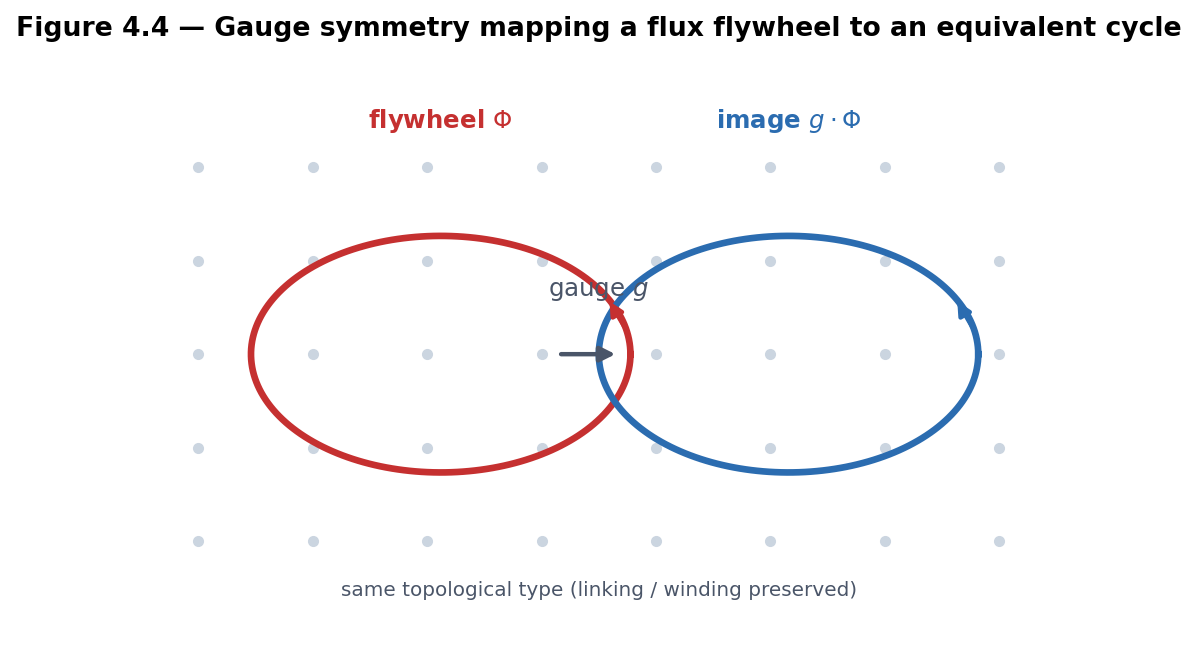
\includegraphics[width=0.92\textwidth,height=0.42\textheight,keepaspectratio]{fig4_4_symmetry_on_flywheel.png}
  \caption{Figure 4.4 --- Gauge symmetry preserving a flux flywheel.}
  \label{fig:fig4-4-symmetry-on-flywheel}
\end{figure}

\begin{quote}\small\textit{Figure 4.4.* A gauge transformation maps a closed circulating flux cycle to another cycle of the same topological type. In the \textbf{Model}, flywheels are equivariant under the symmetry group developed here---exactly the structure Chapter 5 will demand of flux topographs.}\end{quote}

\subsection{Dynamical gauge (\textbf{software} / \textbf{Model})}
\label{ch:ch04_symmetries:dynamical-gauge-software-model}

In \texttt{TwoGyroLattice}, each frame applies left/right rotors and a global right-type gauge rotation driven by mean twist. \textbf{Identity preservation} is a numerical proxy for ``how well the gauged configuration remembers its initial orientation.'' Stable vs chaotic modes (Ch. 3 Aux A3.1) are dynamical illustrations of ordered vs disordered gauge orbits---not combinatorial periods on \(\Lambda_0\).

\bigskip
\noindent\rule{\textwidth}{0.4pt}
\bigskip

\section{4.5 First computational labs}
\label{ch:ch04_symmetries:4-5-first-computational-labs}

\begin{lstlisting}[style=qga]
qga/lib/hopf_lattice.py
  left_multiply, right_multiply, phase_unit,
  apply_gauge_sequence, orbit_of_point,
  permutes_hurwitz_units, adjacency_equivariance_score,
  discrete_flux_cycle, transform_flux

kingdom.core.lattice.LatticeConfig
kingdom.simulations.lattice.TwoGyroLattice   # step_frame(), not step()
\end{lstlisting}

\subsection{Lab 4.A --- Discrete gauge actions on Hurwitz units}
\label{ch:ch04_symmetries:lab-4-a-discrete-gauge-actions-on-hurwitz-units}

\begin{lstlisting}[style=qga,language=python]
import sys
from pathlib import Path
sys.path.insert(0, str(Path.home() / "Projects" / "qga"))

from lib.hopf_lattice import (
    HURWITZ_UNITS, left_multiply, hopf_project_points, permutes_hurwitz_units,
)
import numpy as np

i = np.array([0.0, 1.0, 0.0, 0.0])
print("left permutes units?", permutes_hurwitz_units(i, side="L"))
print("right permutes units?", permutes_hurwitz_units(i, side="R"))

base0 = hopf_project_points(HURWITZ_UNITS)
moved = left_multiply(HURWITZ_UNITS, i)
baseL = hopf_project_points(moved)

# 1) The *set* of base points is invariant (permutation of ??)
rounded0 = np.round(base0, decimals=6)
roundedL = np.round(baseL, decimals=6)
same_set = np.array_equal(
    np.sort(rounded0, axis=0),
    np.sort(roundedL, axis=0),
)
print("Base point set is invariant under left multiplication by i:", same_set)

# 2) The action is still non-trivial on the total space (points are permuted)
print("Any total-space point moved (index-wise)?",
      not np.allclose(moved, HURWITZ_UNITS))
print("max total-space displacement (index-wise):",
      np.max(np.linalg.norm(moved - HURWITZ_UNITS, axis=1)))

# 3) Index-wise base images may or may not change (depends on unit and fiber)
print("Any base coordinate moved (index-wise)?", not np.allclose(base0, baseL))
\end{lstlisting}

\textbf{Note.} Because left multiplication by a Hurwitz unit is a group action on the finite set \(\Lambda_0\), the projected base points are merely \textbf{permuted}. A sorted comparison of base coordinates therefore returns (approximately) equal---that is the expected signature of a \textbf{symmetry}, not a bug. Non-triviality shows up clearly in the \textbf{total space}: index-wise quaternions move (a permutation of the 24 units). Index-wise base coordinates may stay put for some units (e.g. left multiplication by \(i\) can preserve \(h(q)\) along certain fibers) even while the underlying lattice points are swapped---another reminder that the Hopf map collapses whole circles.

\subsection{Lab 4.B --- Generate an orbit under a gauge sequence}
\label{ch:ch04_symmetries:lab-4-b-generate-an-orbit-under-a-gauge-sequence}

\begin{lstlisting}[style=qga,language=python]
from lib.hopf_lattice import HURWITZ_UNITS, orbit_of_point, phase_unit
import numpy as np

i = np.array([0.0, 1.0, 0.0, 0.0])
j = np.array([0.0, 0.0, 1.0, 0.0])
seq = [("R", phase_unit(np.pi / 3)), ("L", i), ("R", phase_unit(np.pi / 3)), ("L", j)]
orbit = orbit_of_point(HURWITZ_UNITS[3], seq, max_periods=24, tol=1e-6)
print("orbit sample count (incl. start):", len(orbit))
print("return distance:", np.linalg.norm(orbit[-1] - orbit[0]))
\end{lstlisting}

\subsection{Lab 4.C --- Dynamical gauge evolution (portal)}
\label{ch:ch04_symmetries:lab-4-c-dynamical-gauge-evolution-portal}

\begin{lstlisting}[style=qga,language=python]
from kingdom.core.lattice import LatticeConfig
from kingdom.simulations.lattice import TwoGyroLattice

config = LatticeConfig(n_sites=48, gauge_strength=0.7, frames=60)
lattice = TwoGyroLattice(config, mode="stable")
for _ in range(60):
    lattice.step_frame()  # note: step_frame, not step
print("final identity preservation:", lattice.identity_preservation[-1])
print("final gauge pointer:", lattice.pointer_history[-1])
\end{lstlisting}

Compare with \texttt{mode="chaotic"} or \texttt{run\_lattice\_comparison}. Observe periodic versus disordered long-term behavior in the Gradio \textbf{Lattice Simulator} tab.

\subsection{Lab 4.D --- Symmetry action on a toy flux cycle}
\label{ch:ch04_symmetries:lab-4-d-symmetry-action-on-a-toy-flux-cycle}

\begin{lstlisting}[style=qga,language=python]
from lib.hopf_lattice import (
    sample_angle_lattice, candidate_adjacency, discrete_flux_cycle,
    left_multiply, nearest_index_map, transform_flux,
)
import numpy as np

pts = sample_angle_lattice(n_eta=2, n_xi1=6, n_xi2=8)
along, inter = candidate_adjacency(pts, base_angle_thresh=0.55, fiber_phase_bins=8)
edges = along[:8] if along else inter[:8]
Phi = discrete_flux_cycle(edges, value=1)
i = np.array([0.0, 1.0, 0.0, 0.0])
moved = left_multiply(pts, i)
# index map: each old vertex index -> nearest image index in moved cloud
# (for pure left mult. with shared indexing, map is identity on indices)
imap = {k: k for k in range(len(pts))}
Phi2 = transform_flux(Phi, imap)
print("flux edges:", len(Phi) // 2, "->", len(Phi2) // 2)
# OP1: does adjacency type survive?
from lib.hopf_lattice import adjacency_equivariance_score
print(adjacency_equivariance_score(pts, i, side="L", base_angle_thresh=0.55, fiber_phase_bins=8))
\end{lstlisting}

\bigskip
\noindent\rule{\textwidth}{0.4pt}
\bigskip

\section{Exercises}
\label{ch:ch04_symmetries:exercises}

\textbf{4.A (hand).} Prove that left multiplication by a unit quaternion is an isometry of \(S^3\) (preserve \(N(uq)=N(u)N(q)=N(q)\)).

\textbf{4.B (hand).} In one paragraph, explain why right multiplication by \(e^{i\phi}\) (embedded as a unit quaternion) implements the structure-group action of the Hopf bundle in the classical complex picture.

\textbf{4.C (code).} Complete Lab 4.A. Confirm \texttt{permutes\_hurwitz\_units} for several Hurwitz units on both left and right. For each unit, report: (i) sorted base multiset invariant? (ii) total-space index-wise motion? (iii) base index-wise motion?

\textbf{4.D (code).} Complete Lab 4.B. Find a short non-trivial sequence that returns (approximately) to the start; report period length.

\textbf{4.E (visual / dynamical).} Run Lab 4.C or the Lattice Simulator. Identify visibly ordered gauge-pointer behavior and contrast it with chaotic regimes.

\textbf{4.F (Hatcher bridge).} In Hatcher, the translation \(T_n(z)=z+n\) generates periodic strips. Construct a quaternionic analogue (repeated right phase advance + compensating left shift) on a small angle lattice and describe the base track (cf. Fig. 4.3).

\textbf{4.G (forward).} Why must any flux topograph defined in Chapter 5 be equivariant under the gauge actions studied here?

\textbf{4.H (Open Problem 1 connection).} Using \texttt{adjacency\_equivariance\_score}, test whether \texttt{candidate\_adjacency} is preserved by left and right multiplications by a few Hurwitz units on \(\Lambda_{\mathrm{ang}}\). Record failures---they constrain what a canonical rule can be.

\textbf{4.I (software honesty).} In two sentences, distinguish combinatorial periods on \(\Lambda_0\) from dynamical `\texttt{identity preservation'' in }TwoGyroLattice`. Which claim type applies to each?

\bigskip
\noindent\rule{\textwidth}{0.4pt}
\bigskip

\section{Code and asset pointers}
\label{ch:ch04_symmetries:code-and-asset-pointers}

\begin{lstlisting}[style=qga]
qga/lib/hopf_lattice.py
kingdom.core.lattice.LatticeConfig
kingdom.simulations.lattice.TwoGyroLattice
kingdom.simulations.lattice.run_lattice_comparison
kingdom.core.hopf
\end{lstlisting}

\textbf{Figures:} \texttt{scripts/generate\_ch4\_figures.py} \textbf{Related portal:} Lattice Simulator tab --- dynamical illustration of gauge evolution and identity preservation. \textbf{Open problems:} OP1 equivariance tests (Exercise 4.H); see \texttt{notes/open\_problems.md}.

\bigskip
\noindent\rule{\textwidth}{0.4pt}
\bigskip

\section{Looking ahead}
\label{ch:ch04_symmetries:looking-ahead}

The gauge symmetries of the gauged Hopf lattice are now operational: left and right multiplications generate a rich group whose action mirrors (in the \textbf{Model} sense) the modular group on Hatcher's Farey diagram. In \textbf{Chapter 5} we lift Conway's topographs to this setting, producing \textbf{flux topographs} whose value landscapes, separator structures, and periodicity will be required to be equivariant under the symmetries developed here. Classification, Magic Islands, and the \(Z\mapsto\) flywheel map will follow from the reduced configurations and periodic orbits these symmetries make visible.

With the lattice and its symmetries in place, we are ready to develop the visual and arithmetic theory of flux topographs---the direct quaternionic descendant of Hatcher's topographs of binary quadratic forms.

\bigskip
\noindent\rule{\textwidth}{0.4pt}
\bigskip




\part{Forms, Topographs, and Representations}
% Auto-generated from book/05_forms_topographs.md — do not edit by hand
% Regenerated by scripts/md_to_latex.py

\chapter{Chapter 5 --- Quaternionic Forms and Flux Topographs}
\label{ch:ch05_topographs}

This chapter lifts Conway's topographs of binary quadratic forms (Hatcher Chapters 4--5) to the gauged Hopf lattice. We define \textbf{flux topographs}---value landscapes on the discrete lattice whose periodic separator structures encode stability, periodicity, and classification. The resulting theory is the direct higher-dimensional, quaternionic analogue of Hatcher's visual number theory, with Magic Islands as a natural generalization of class-number phenomena and reduced forms---stated carefully as a \textbf{Model}.

\textbf{Learning goals}

\begin{enumerate}
\item Generalize binary quadratic forms and their topographs to flux functionals on the gauged Hopf lattice.  
\item Define flux topographs, value landscapes, and separator structures.  
\item Understand periodicity, reduced configurations, and Magic Islands.  
\item See how gauge symmetries act on topographs (equivariance).  
\item Prepare the visual and arithmetic foundation for classification (Chapter 6) and the \(Z\mapsto\) flywheel map (Chapter 7).
\end{enumerate}

\textbf{Figures in this chapter}

\begin{center}
\small
\setlength{\tabcolsep}{4pt}
\begin{tabularx}{\textwidth}{@{}>{\raggedright\arraybackslash}p{0.12\textwidth}>{\raggedright\arraybackslash}X>{\raggedright\arraybackslash}X@{}}
\toprule
Tag & File & Role \\
\midrule
Fig. 5.1 & \texttt{figures/\allowbreak{}fig5\_\allowbreak{}1\_\allowbreak{}flux\_\allowbreak{}topograph\_\allowbreak{}schematic.\allowbreak{}png} & Flux topograph value landscape \\
Fig. 5.2 & \texttt{figures/\allowbreak{}fig5\_\allowbreak{}2\_\allowbreak{}separator\_\allowbreak{}structure.\allowbreak{}png} & Periodic / sign-crossing separators \\
Fig. 5.3 & \texttt{figures/\allowbreak{}fig5\_\allowbreak{}3\_\allowbreak{}magic\_\allowbreak{}island.\allowbreak{}png} & Magic Island schematic + model Z-sweep \\
Fig. 5.4 & \texttt{figures/\allowbreak{}fig5\_\allowbreak{}4\_\allowbreak{}symmetry\_\allowbreak{}on\_\allowbreak{}topograph.\allowbreak{}png} & Gauge action on a topograph \\
Aux A5.1 & \texttt{figures/\allowbreak{}aux5\_\allowbreak{}1\_\allowbreak{}topograph\_\allowbreak{}evolution.\allowbreak{}png} & Evolution under repeated right phase \\
\bottomrule
\end{tabularx}
\end{center}


\textbf{Claim discipline}

\begin{center}
\small
\setlength{\tabcolsep}{4pt}
\begin{tabularx}{\textwidth}{@{}>{\raggedright\arraybackslash}X>{\raggedright\arraybackslash}X@{}}
\toprule
Claim & Type \\
\midrule
Classical topograph properties (periodicity, arithmetic progression rule, reduced forms) from Hatcher & \textbf{Theorem} (classical; cited) \\
Flux topographs, separator structures, Magic Islands, gauge equivariance of candidate constructions & \textbf{Model} (core of OP2) \\
\texttt{qga/\allowbreak{}lib/\allowbreak{}flux\_\allowbreak{}topograph.\allowbreak{}py}, \texttt{kingdom.\allowbreak{}core.\allowbreak{}flux\_\allowbreak{}flywheel} APIs & \textbf{Software fact} \\
\bottomrule
\end{tabularx}
\end{center}


\bigskip
\noindent\rule{\textwidth}{0.4pt}
\bigskip

\section{5.1 From binary quadratic forms to flux functionals}
\label{ch:ch05_topographs:5-1-from-binary-quadratic-forms-to-flux-functionals}

In Hatcher, a binary quadratic form

\[
f(x,y) = ax^2 + bxy + cy^2
\]

acquires a \textbf{topograph}---a value landscape drawn on the dual of the Farey triangulation. Adjacent regions differ by an arithmetic progression rule, and periodic separator lines appear for indefinite forms (positive non-square discriminant).

We lift this picture to the gauged Hopf lattice of Chapters 3--4:

A \textbf{flux functional} on the lattice assigns a real (or integer) value to vertices---and, in richer versions, to edges or small cycles---such that the assignment transforms naturally under gauge actions. A \textbf{flux topograph} is the visual landscape of these values together with their level sets and separator structures.

Natural candidate functionals (all \textbf{Model} choices for OP2 experiments):

\begin{center}
\small
\setlength{\tabcolsep}{4pt}
\begin{tabularx}{\textwidth}{@{}>{\raggedright\arraybackslash}X>{\raggedright\arraybackslash}X@{}}
\toprule
Name (book helper) & Geometric meaning \\
\midrule
\texttt{norm} & \(x^2+y^2+z^2\) on pure-imaginary part (quadratic form on \(\mathrm{Im}\,\mathbb{H}\)) \\
\texttt{hopf\_\allowbreak{}y1} / \texttt{hopf\_\allowbreak{}height} & Classical Hopf base coordinates (Ch. 2) \\
\texttt{phase} & Fiber phase proxy \(\mathrm{atan2}(x_4,x_3)\) \\
portal stability & \texttt{map\_\allowbreak{}z\_\allowbreak{}to\_\allowbreak{}flywheel} scores (Ch. 7 preview) \\
\bottomrule
\end{tabularx}
\end{center}


\textbf{Model note.} The precise choice of functional is part of the definition of flux topographs and is tied to \textbf{Open Problem 2}. No uniqueness claim is made in this chapter.

\bigskip
\noindent\rule{\textwidth}{0.4pt}
\bigskip

\section{5.2 Flux topographs and separator structures}
\label{ch:ch05_topographs:5-2-flux-topographs-and-separator-structures}

\subsection{Definition (working)}
\label{ch:ch05_topographs:definition-working}

A \textbf{flux topograph} is a tuple

\[
\bigl(\Lambda,\; E,\; V,\; \mathcal{S}\bigr)
\]

where \(\Lambda\) is a discrete point set in \(S^3\), \(E\) is an edge set (along-fiber and/or inter-fiber from Ch. 3), \(V:\Lambda\to\mathbb{R}\) is a flux functional, and \(\mathcal{S}\) is the separator structure extracted from \(V\) (sign crossings, critical levels).

In code:

\begin{lstlisting}[style=qga]
FluxTopograph(points, values, edges, functional)
build_flux_topograph(points, edges=..., functional=...)
detect_separators(topo, threshold=..., mode='sign'|'level')
\end{lstlisting}

\begin{figure}[htbp]
  \centering
  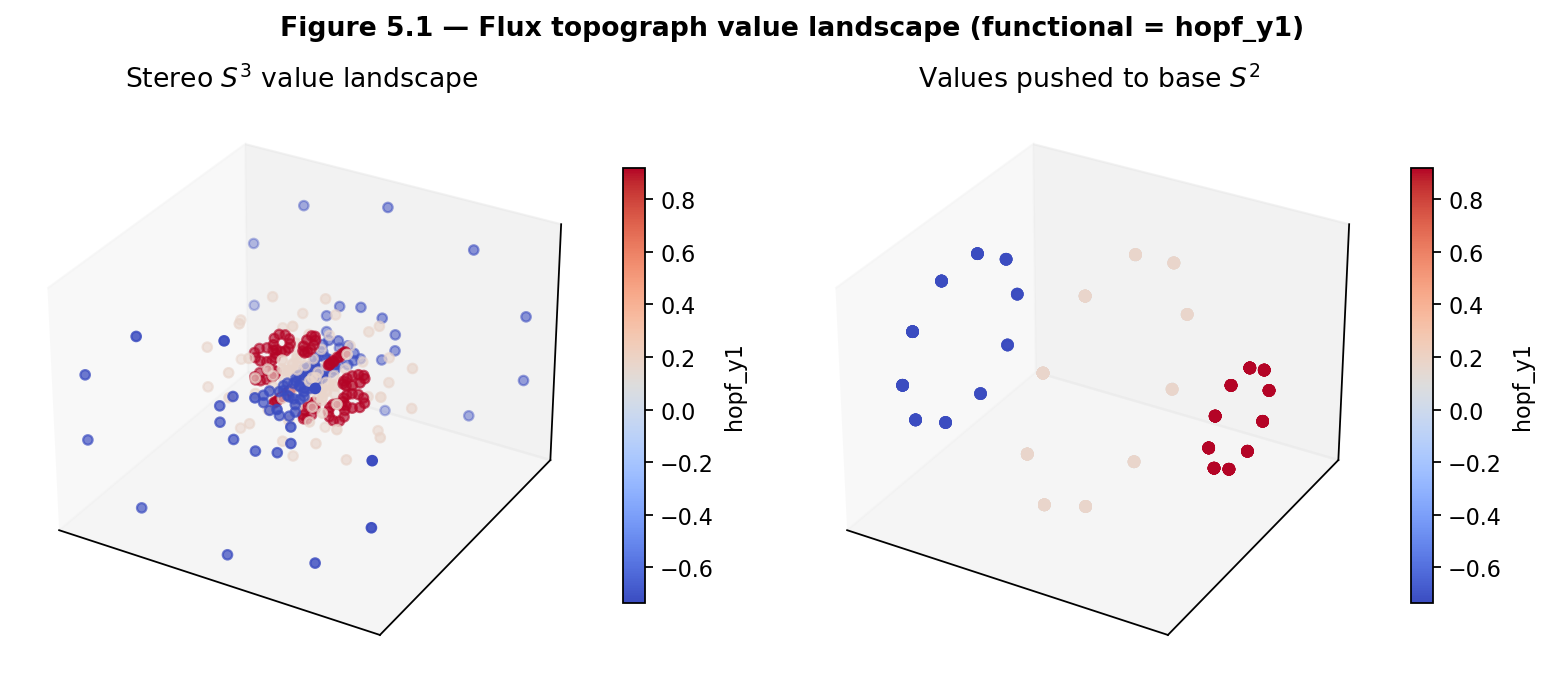
\includegraphics[width=0.92\textwidth,height=0.42\textheight,keepaspectratio]{fig5_1_flux_topograph_schematic.png}
  \caption{Figure 5.1 --- Flux topograph value landscape.}
  \label{fig:fig5-1-flux-topograph-schematic}
\end{figure}

\begin{quote}\small\textit{Figure 5.1.* Value landscape for the functional \texttt{hopf\_\allowbreak{}y1} on an angle-sampled lattice, shown in stereographic \(S^3\) and pushed to the base \(S^2\).}\end{quote}

\subsection{Separator structures}
\label{ch:ch05_topographs:separator-structures}

\textbf{Separator structures} are the loci where the functional changes sign or crosses a critical threshold. On a graph, they appear as edges \((i,j)\) with \(V(i)\) and \(V(j)\) on opposite sides of a threshold. Connected components of those edges are discrete analogues of Hatcher's separator curves.

In the indefinite / oscillatory case, separators can become \textbf{periodic} under the gauge group---exactly analogous to Hatcher's periodic separator lines for indefinite binary forms, which encode infinitude (Pell-type families).

\begin{figure}[htbp]
  \centering
  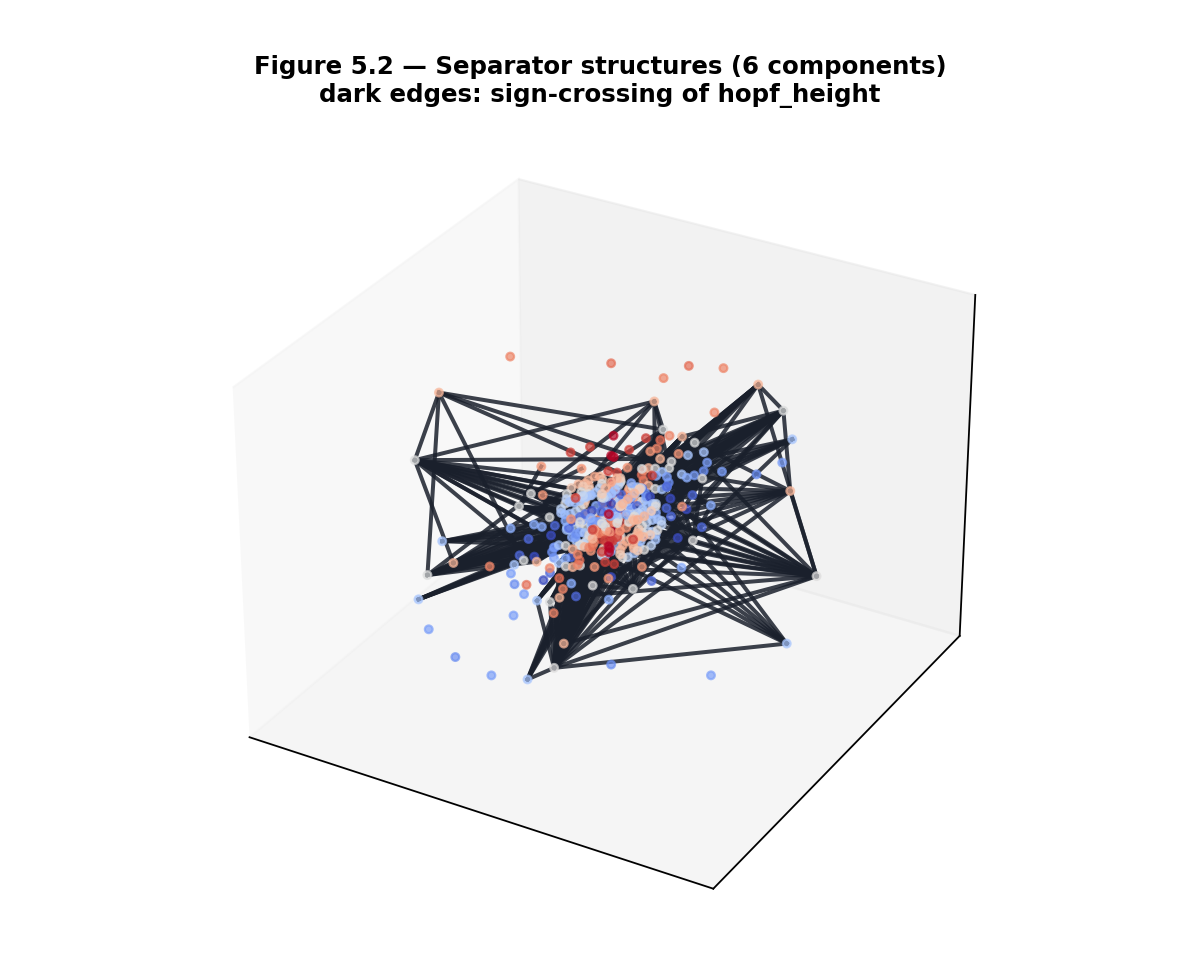
\includegraphics[width=0.92\textwidth,height=0.42\textheight,keepaspectratio]{fig5_2_separator_structure.png}
  \caption{Figure 5.2 --- Separator structures.}
  \label{fig:fig5-2-separator-structure}
\end{figure}

\begin{quote}\small\textit{Figure 5.2.* Dark edges: sign-crossing separators of \texttt{hopf\_\allowbreak{}height} on the candidate adjacency graph. Component count and edge sets are experimental OP2 diagnostics, not theorems.}\end{quote}

\subsection{Arithmetic progression rule (lift)}
\label{ch:ch05_topographs:arithmetic-progression-rule-lift}

Classically, values on three regions meeting at a topograph edge satisfy a linear relation (Hatcher's arithmetic progression rule). On the gauged Hopf lattice we only partially lift this: for each edge we can measure jumps \(V(j)-V(i)\) and study their regularity under gauge moves (\texttt{arithmetic\_\allowbreak{}progression\_\allowbreak{}residuals}). A full equivariant AP rule compatible with quaternion multiplication is part of \textbf{OP2}.

\bigskip
\noindent\rule{\textwidth}{0.4pt}
\bigskip

\section{5.3 Periodicity, reduced configurations, and Magic Islands}
\label{ch:ch05_topographs:5-3-periodicity-reduced-configurations-and-magic-islands}

\subsection{Periodicity under the gauge group}
\label{ch:ch05_topographs:periodicity-under-the-gauge-group}

When a flux topograph is (approximately) periodic under a composite gauge sequence \(g\) from Chapter 4---i.e. \(g^k\cdot\Phi \approx \Phi\) for some \(k\)---the orbit corresponds to a \textbf{reduced configuration}. The book helper \texttt{periodicity\_\allowbreak{}score} reports nearest-neighbor total-space return and multiset distance of values.

\subsection{Magic Islands}
\label{ch:ch05_topographs:magic-islands}

\textbf{Magic Islands} are pockets of enhanced stability in parameter space (detuning \(\delta\omega\), gauge strength, layers, or atomic number \(Z\) in the portal Model). Inside an island the topograph (or the derived stability score) shows strong order: high \texttt{stability\_\allowbreak{}score}, noble-gas locks, low variation. Outside, scores drop and dynamical simulations become more chaotic (Ch. 3 Aux A3.1).

They are the narrative generalization of finite class number and reduced forms in Hatcher's theory. \textbf{Arithmetic characterization} (class-number-like invariants predicting islands) is deferred to Open Problem 3 / Chapter 6.

\begin{figure}[htbp]
  \centering
  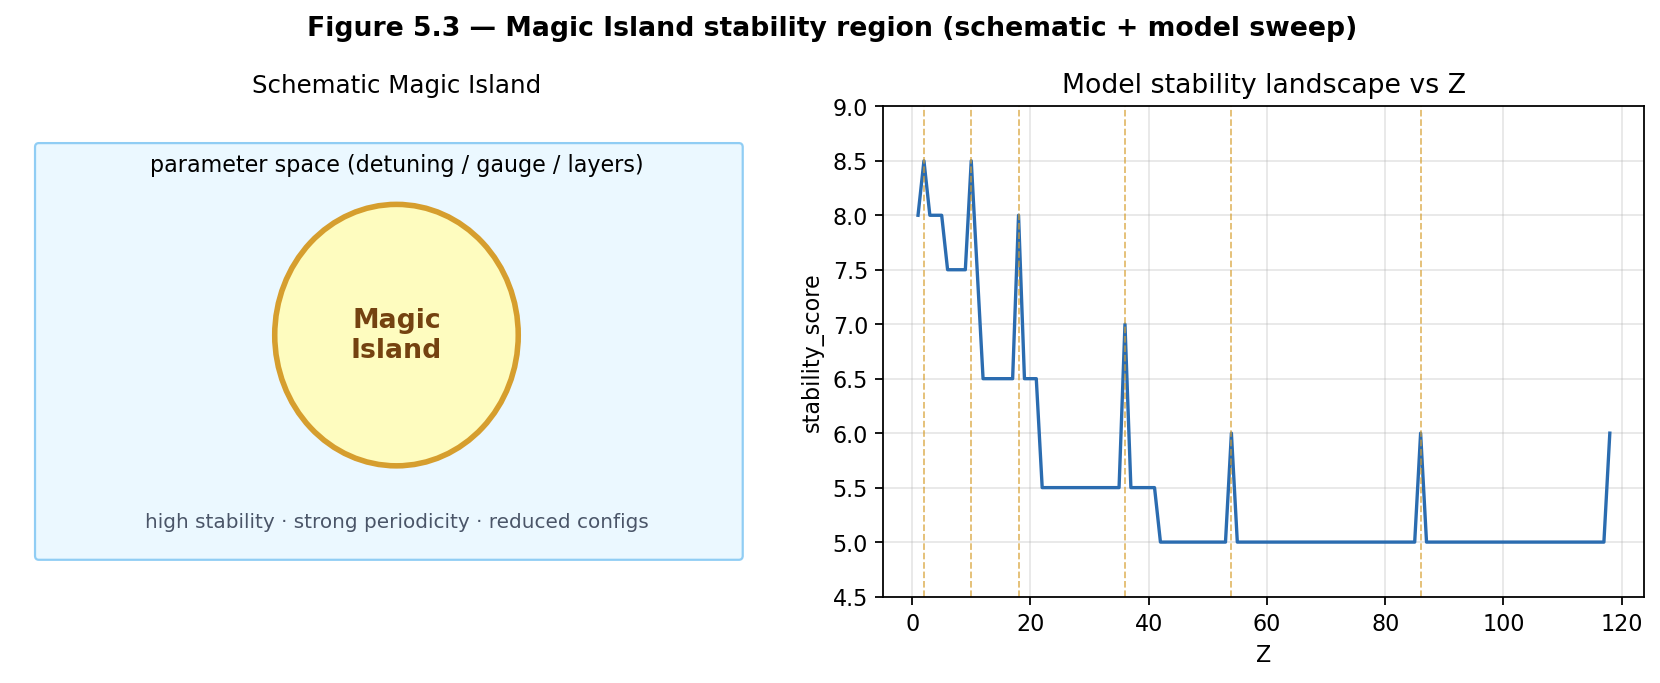
\includegraphics[width=0.92\textwidth,height=0.42\textheight,keepaspectratio]{fig5_3_magic_island.png}
  \caption{Figure 5.3 --- Magic Island stability region.}
  \label{fig:fig5-3-magic-island}
\end{figure}

\begin{quote}\small\textit{Figure 5.3.* Left: schematic island in parameter space. Right: Kingdom Come Model \texttt{stability\_\allowbreak{}score} vs \(Z\) (gold lines mark noble-gas \(Z\)). \textbf{Software fact} for the right panel; physical interpretation remains \textbf{Model}.}\end{quote}

\textbf{Claim type.} Visual and software properties of Magic Islands in the portal: \textbf{Model} + \textbf{Software fact}. Classical reduced forms / class number: \textbf{Theorem} (Hatcher). Correspondence between the two: \textbf{Open} (OP3).

\bigskip
\noindent\rule{\textwidth}{0.4pt}
\bigskip

\section{5.4 Gauge equivariance of flux topographs}
\label{ch:ch05_topographs:5-4-gauge-equivariance-of-flux-topographs}

Any well-defined flux topograph must be \textbf{equivariant} under the gauge group of Chapter 4: applying a left or right multiplication must map the topograph to another topograph of the same type (possibly after transporting values or recomputing a geometric functional).

This is the direct analogue of Hatcher's requirement that topographs transform properly under linear fractional transformations.

\begin{figure}[htbp]
  \centering
  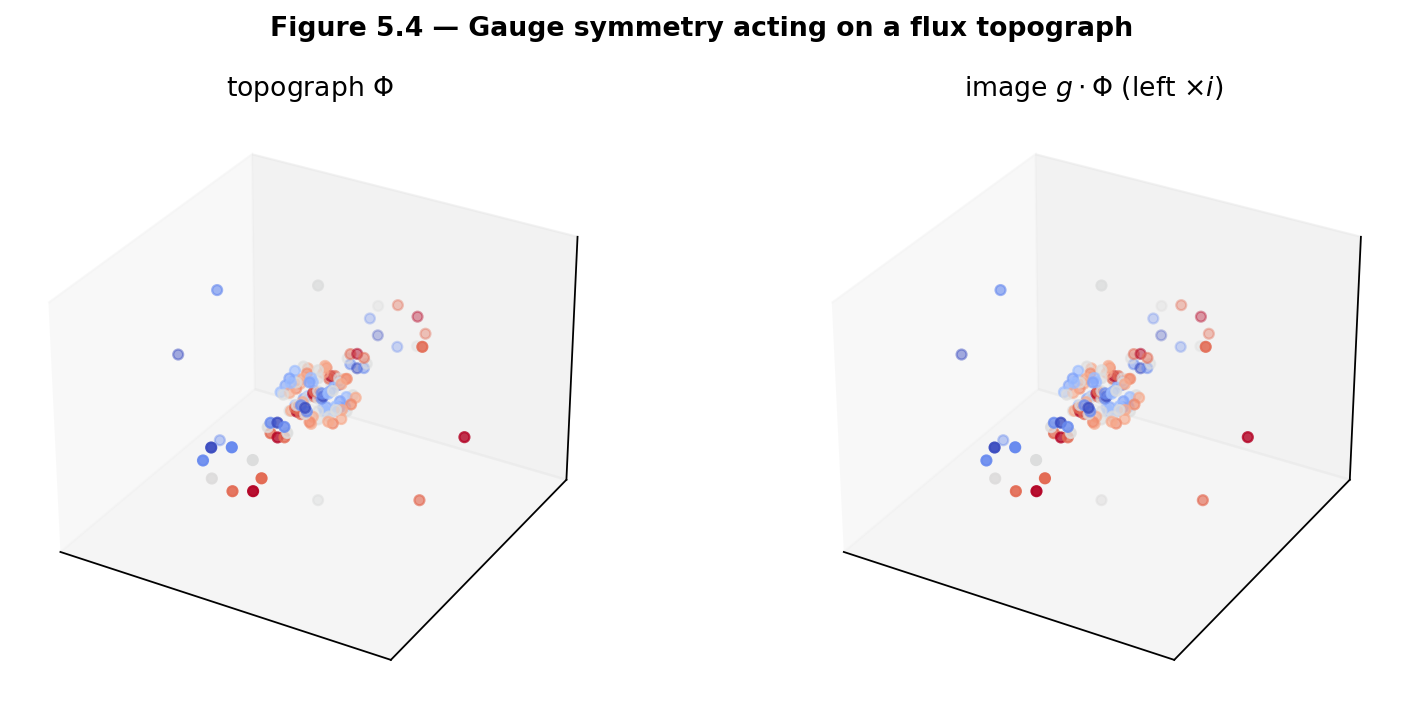
\includegraphics[width=0.92\textwidth,height=0.42\textheight,keepaspectratio]{fig5_4_symmetry_on_topograph.png}
  \caption{Figure 5.4 --- Gauge symmetry acting on a flux topograph.}
  \label{fig:fig5-4-symmetry-on-topograph}
\end{figure}

\begin{quote}\small\textit{Figure 5.4.* Left multiplication by \(i\) maps a \texttt{hopf\_\allowbreak{}y1} topograph to its image. For geometric functionals recomputed after the move, values track the geometry exactly.}\end{quote}

\begin{figure}[htbp]
  \centering
  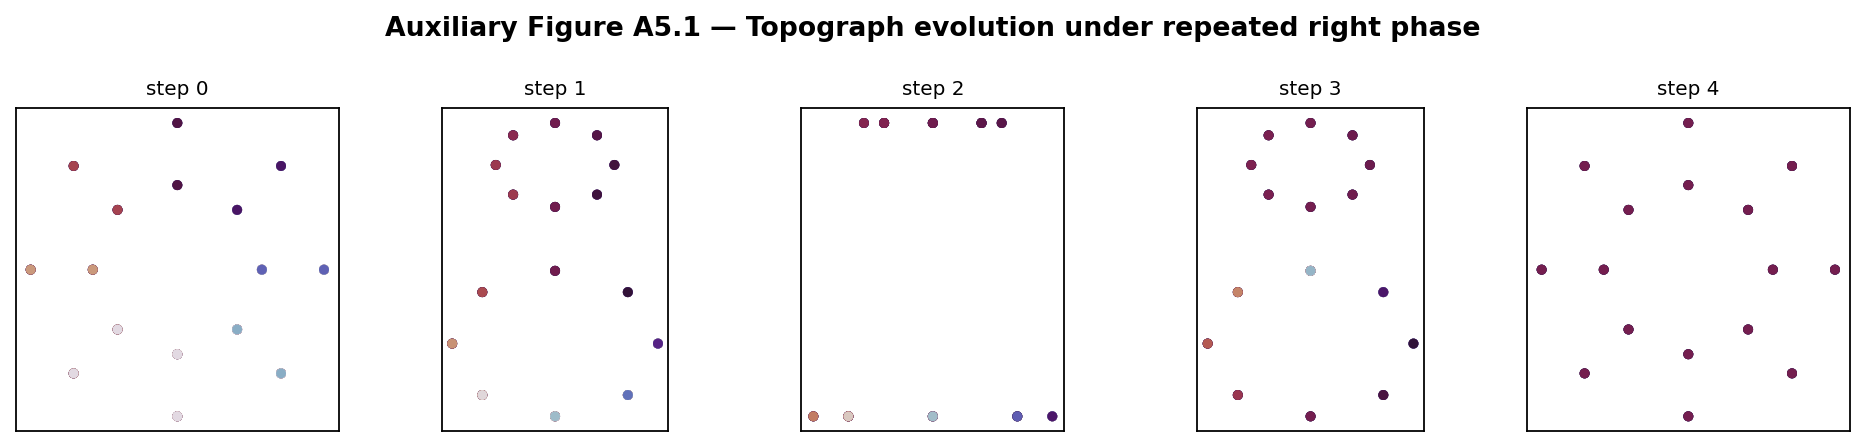
\includegraphics[width=0.92\textwidth,height=0.42\textheight,keepaspectratio]{aux5_1_topograph_evolution.png}
  \caption{Auxiliary Figure A5.1 --- Topograph evolution.}
  \label{fig:aux5-1-topograph-evolution}
\end{figure}

\begin{quote}\small\textit{Auxiliary Figure A5.1.* Repeated right phase advances: base scatter colored by \texttt{phase} functional. Separator patterns should transform predictably if OP2 axioms hold.}\end{quote}

\textbf{Open Problem 2 (core of this chapter).} Formalize the axioms of a flux topograph so that:

\begin{enumerate}
\item The structure \textbf{reduces} to Conway/Hatcher topographs under a suitable projection or restriction.  
\item Separator periodicity and an arithmetic progression rule lift naturally.  
\item \textbf{Gauge equivariance} holds for a fixed adjacency rule from Chapter 3 (OP1).  
\item Magic Islands emerge as finite or periodic reduced regions with measurable stability.
\end{enumerate}

\textbf{Sandbox:} \texttt{qga/\allowbreak{}lib/\allowbreak{}flux\_\allowbreak{}topograph.\allowbreak{}py} --- \texttt{build\_\allowbreak{}flux\_\allowbreak{}topograph}, \texttt{detect\_\allowbreak{}separators}, \texttt{periodicity\_\allowbreak{}score}, \texttt{separator\_\allowbreak{}equivariance\_\allowbreak{}score}.

\bigskip
\noindent\rule{\textwidth}{0.4pt}
\bigskip

\section{5.5 First computational labs}
\label{ch:ch05_topographs:5-5-first-computational-labs}

Helpers: \texttt{lib/\allowbreak{}flux\_\allowbreak{}topograph.\allowbreak{}py} \(\cdot\) portal: \texttt{map\_\allowbreak{}z\_\allowbreak{}to\_\allowbreak{}flywheel} \(\cdot\) \textbf{Appendix C ?C.3}.

\begin{itemize}
\item \textbf{5.A} \texttt{build\_\allowbreak{}flux\_\allowbreak{}topograph} + \texttt{detect\_\allowbreak{}separators}.
\item \textbf{5.B} \texttt{periodicity\_\allowbreak{}score} under a gauge sequence.
\item \textbf{5.C} Z-stability via \texttt{map\_\allowbreak{}z\_\allowbreak{}to\_\allowbreak{}flywheel} (no \texttt{magic\_\allowbreak{}flag} --- use \texttt{stability\_\allowbreak{}score} / \texttt{is\_\allowbreak{}noble\_\allowbreak{}gas}).
\item \textbf{5.D} \texttt{separator\_\allowbreak{}equivariance\_\allowbreak{}score} (OP2 diagnostic).
\end{itemize}

\begin{lstlisting}[style=qga,language=python]
from lib.flux_topograph import build_flux_topograph, detect_separators
from lib.hopf_lattice import sample_angle_lattice, candidate_adjacency
pts = sample_angle_lattice(3, 8, 8)
along, inter = candidate_adjacency(pts)
topo = build_flux_topograph(pts, edges=along+inter, functional="hopf_height")
print(len(detect_separators(topo)))
\end{lstlisting}

\bigskip
\noindent\rule{\textwidth}{0.4pt}
\bigskip

\section{Exercises}
\label{ch:ch05_topographs:exercises}

\textbf{5.A (hand).} State the classical arithmetic progression rule for Hatcher topographs (or look it up in TN Ch. 4) and propose a quaternionic lift for flux values on adjacent lattice elements.

\textbf{5.B (hand).} In two sentences, explain why gauge equivariance is a necessary condition for a flux topograph to be well-defined.

\textbf{5.C (code).} Complete Labs 5.A--5.B. Report separator component count and \texttt{periodicity\_\allowbreak{}score} for your functional.

\textbf{5.D (code).} Run Lab 5.C for \(Z\in\{2,10,26,79,118\}\). Which values show high \texttt{stability\_\allowbreak{}score} or \texttt{is\_\allowbreak{}noble\_\allowbreak{}gas=True}? Record the pattern.

\textbf{5.E (visual).} Generate a flux topograph and apply one gauge transformation (Fig. 5.4). Describe how separator curves / value colors transform.

\textbf{5.F (Hatcher bridge).} In Hatcher, reduced forms and class number classify quadratic forms up to equivalence. Sketch how Magic Islands might play an analogous role for flux configurations on the gauged Hopf lattice.

\textbf{5.G (Open Problem 2 teaser).} Using \texttt{build\_\allowbreak{}flux\_\allowbreak{}topograph} and \texttt{detect\_\allowbreak{}separators}, test whether separator counts survive under \texttt{candidate\_\allowbreak{}adjacency} + left/right multiplications (\texttt{separator\_\allowbreak{}equivariance\_\allowbreak{}score}). Document failures---they inform OP2 axioms.

\textbf{5.H (forward).} Why will the classification theory of Chapter 6 depend on the periodic separator structures developed here?

\textbf{5.I (software honesty).} In one paragraph, distinguish: (i) pedagogical flux functionals in \texttt{qga/\allowbreak{}lib/\allowbreak{}flux\_\allowbreak{}topograph.\allowbreak{}py}, (ii) portal \texttt{stability\_\allowbreak{}score} from \texttt{map\_\allowbreak{}z\_\allowbreak{}to\_\allowbreak{}flywheel}, (iii) classical Conway topographs. Assign claim types.

\bigskip
\noindent\rule{\textwidth}{0.4pt}
\bigskip

\section{Code and asset pointers}
\label{ch:ch05_topographs:code-and-asset-pointers}

\begin{lstlisting}[style=qga]
qga/lib/flux_topograph.py
  build_flux_topograph, detect_separators, periodicity_score,
  apply_gauge_to_topograph, separator_equivariance_score,
  arithmetic_progression_residuals, stability_landscape_z

qga/lib/hopf_lattice.py
kingdom.core.flux_flywheel.map_z_to_flywheel[_extended]
kingdom.viz.magic_island.build_magic_island_heatmap
\end{lstlisting}

\textbf{Figures:} \texttt{scripts/\allowbreak{}generate\_\allowbreak{}ch5\_\allowbreak{}figures.\allowbreak{}py} \textbf{Related portal:} Flux Flywheel tab; Magic Island heatmap; Lattice Simulator (dynamical backdrop). \textbf{Open problems:} OP2 (\texttt{notes/\allowbreak{}open\_\allowbreak{}problems.\allowbreak{}md}); depends on OP1 adjacency.

\bigskip
\noindent\rule{\textwidth}{0.4pt}
\bigskip

\section{Looking ahead}
\label{ch:ch05_topographs:looking-ahead}

Flux topographs are the visual and arithmetic heart of Part III---the direct quaternionic lift of Hatcher's topographs, still with \textbf{Model}-level axioms pending OP2. In \textbf{Chapter 6} we classify these topographs, enumerate reduced configurations, and formalize Magic Islands as higher-dimensional analogues of class numbers and reduced forms. \textbf{Chapter 7} connects classified objects to the \(Z\mapsto\) flywheel map, completing the representation-theoretic bridge from number theory to the periodic-table proxy in the Kingdom Come Model.

With flux topographs in hand, we are ready for the classification theory that turns visual landscapes into arithmetic invariants.

\bigskip
\noindent\rule{\textwidth}{0.4pt}
\bigskip



% Auto-generated from book/06_classification.md — do not edit by hand
% Regenerated by scripts/md_to_latex.py

\chapter{Chapter 6 --- Classification of Flux Topographs and Magic Islands}
\label{ch:ch06_classification}

This chapter classifies flux topographs on the gauged Hopf lattice, enumerates reduced configurations, and formalizes \textbf{Magic Islands} as higher-dimensional analogues of class numbers and reduced forms. The theory mirrors Hatcher Chapters 5--6 while remaining a \textbf{Model} construction pending the axioms of Open Problems 2--3.

\textbf{Learning goals}

\begin{enumerate}
\item Classify flux topographs by invariants analogous to discriminant and type (elliptic / hyperbolic / ...).  
\item Define equivalence of topographs under gauge actions.  
\item Enumerate reduced configurations and compute class-number-like invariants.  
\item Formalize Magic Islands as pockets of enhanced periodicity and stability.  
\item Prepare the arithmetic foundation for the \(Z\mapsto\) flywheel map (Chapter 7) and the class-group lift (Chapter 8).
\end{enumerate}

\textbf{Figures in this chapter}

\begin{center}
\small
\setlength{\tabcolsep}{4pt}
\begin{tabularx}{\textwidth}{@{}>{\raggedright\arraybackslash}p{0.12\textwidth}>{\raggedright\arraybackslash}X>{\raggedright\arraybackslash}X@{}}
\toprule
Tag & File & Role \\
\midrule
Fig. 6.1 & \texttt{figures/\allowbreak{}fig6\_\allowbreak{}1\_\allowbreak{}four\_\allowbreak{}types.\allowbreak{}png} & Four types of flux topographs (schematic) \\
Fig. 6.2 & \texttt{figures/\allowbreak{}fig6\_\allowbreak{}2\_\allowbreak{}reduced\_\allowbreak{}config.\allowbreak{}png} & Reduced configuration (minimal-variance rep) \\
Fig. 6.3 & \texttt{figures/\allowbreak{}fig6\_\allowbreak{}3\_\allowbreak{}class\_\allowbreak{}number\_\allowbreak{}analogue.\allowbreak{}png} & Class-number-like count of reduced islands \\
Fig. 6.4 & \texttt{figures/\allowbreak{}fig6\_\allowbreak{}4\_\allowbreak{}equivalence.\allowbreak{}png} & Gauge equivalence of two topographs \\
Aux A6.1 & \texttt{figures/\allowbreak{}aux6\_\allowbreak{}1\_\allowbreak{}island\_\allowbreak{}sweep.\allowbreak{}png} & Z-sweep revealing Magic-Island-like peaks \\
\bottomrule
\end{tabularx}
\end{center}


\textbf{Claim discipline}

\begin{center}
\small
\setlength{\tabcolsep}{4pt}
\begin{tabularx}{\textwidth}{@{}>{\raggedright\arraybackslash}X>{\raggedright\arraybackslash}X@{}}
\toprule
Claim & Type \\
\midrule
Classical classification of quadratic forms and topographs (Hatcher Ch. 5) & \textbf{Theorem} (cited) \\
Flux topograph types, equivalence, reduced configurations, Magic Islands & \textbf{Model} (core of OP3; depends on OP2) \\
\texttt{qga/\allowbreak{}lib/\allowbreak{}flux\_\allowbreak{}topograph.\allowbreak{}py} classification helpers; Kingdom Come \texttt{stability\_\allowbreak{}score} & \textbf{Software fact} \\
\bottomrule
\end{tabularx}
\end{center}


\bigskip
\noindent\rule{\textwidth}{0.4pt}
\bigskip

\section{6.1 The four types of flux topographs}
\label{ch:ch06_classification:6-1-the-four-types-of-flux-topographs}

In Hatcher, binary quadratic forms (and their topographs) are classified by the sign of the discriminant \(\Delta = b^2-4ac\):

\begin{center}
\small
\setlength{\tabcolsep}{4pt}
\begin{tabularx}{\textwidth}{@{}>{\raggedright\arraybackslash}p{0.12\textwidth}>{\raggedright\arraybackslash}X>{\raggedright\arraybackslash}X@{}}
\toprule
Discriminant & Classical type & Topograph character \\
\midrule
\(\Delta>0\) nonsquare & hyperbolic & periodic separators \\
\(\Delta>0\) square & 0-hyperbolic / parabolic edge & degenerate \\
\(\Delta<0\) & elliptic & finite reduced forms \\
\(\Delta=0\) & parabolic & boundary / degenerate \\
\bottomrule
\end{tabularx}
\end{center}


We lift this classification to flux topographs by examining the flux functional \(V\) and its separator structures under the gauge group of Chapter 4---\textbf{not} by computing a classical \(\Delta\) (that remains OP2--3 territory).

\begin{center}
\small
\setlength{\tabcolsep}{4pt}
\begin{tabularx}{\textwidth}{@{}>{\raggedright\arraybackslash}X>{\raggedright\arraybackslash}X>{\raggedright\arraybackslash}X>{\raggedright\arraybackslash}X@{}}
\toprule
Type & Separator behavior & Reduced configurations & Magic Island character \\
\midrule
Hyperbolic & Periodic separators under gauge & Infinite / periodic families & Large stable islands \\
Elliptic & Finite / bounded separators & Finite reduced set & Compact high-stability pockets \\
Parabolic & Degenerate / transitional separators & Marginal cases & Boundary regions \\
0-hyperbolic & Flat or near-constant regions & Trivial / degenerate & Noble-gas-like locks \\
\bottomrule
\end{tabularx}
\end{center}


\begin{figure}[htbp]
  \centering
  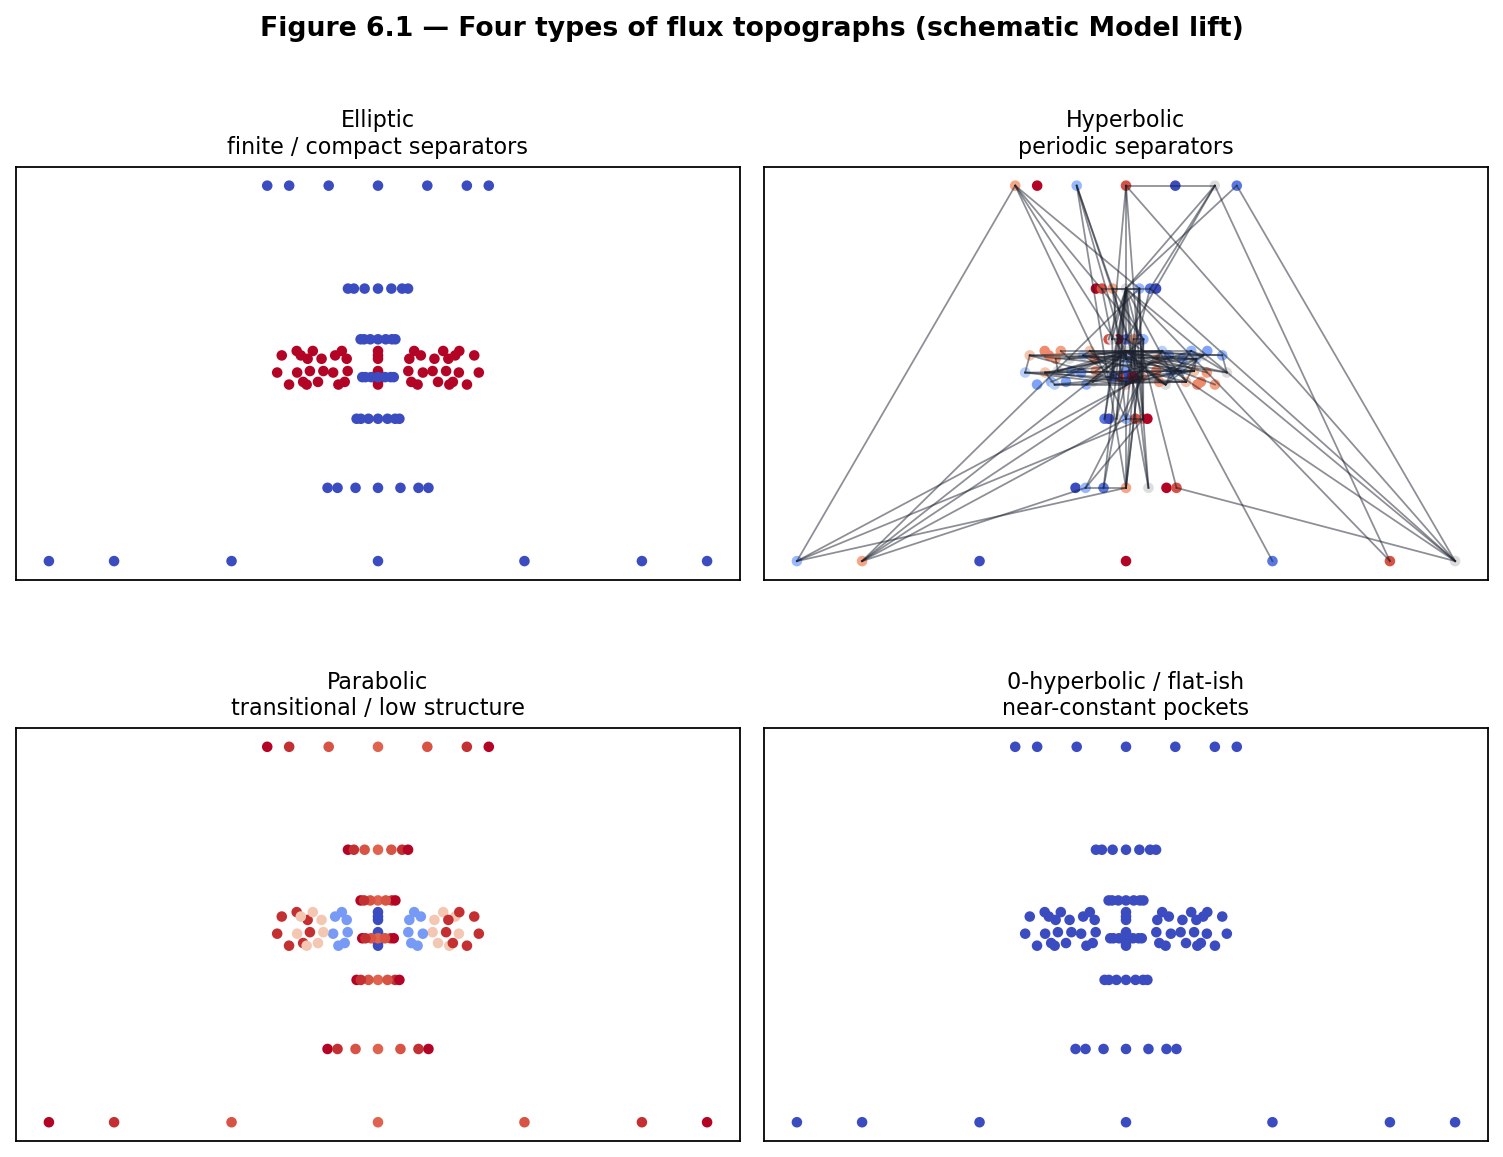
\includegraphics[width=0.92\textwidth,height=0.42\textheight,keepaspectratio]{fig6_1_four_types.png}
  \caption{Figure 6.1 --- Four types of flux topographs (schematic).}
  \label{fig:fig6-1-four-types}
\end{figure}

\begin{quote}\small\textit{Figure 6.1.* Schematic value landscapes and separator patterns for the four lifted types. Generated with pedagogical functionals; labels are Model categories.}\end{quote}

\subsection{Heuristic classifier (software / Model)}
\label{ch:ch06_classification:heuristic-classifier-software-model}

\begin{lstlisting}[style=qga]
classify_topograph_type(topo) ->
  type, reason, n_separator_edges, value_variance,
  best_period_found, signature, ...
\end{lstlisting}

The decision tree (explicitly heuristic) uses:

\begin{enumerate}
\item near-constant values \(\rightarrow\) \texttt{0-hyperbolic}  
\item no sign separators + low variance \(\rightarrow\) \texttt{parabolic}  
\item periodic under a small gauge dictionary + separators \(\rightarrow\) \texttt{hyperbolic}  
\item few separator components \(\rightarrow\) \texttt{elliptic}  
\item otherwise transitional \texttt{parabolic}
\end{enumerate}

This is \textbf{not} a theorem of classification---only a lab tool for OP3 experiments.

\bigskip
\noindent\rule{\textwidth}{0.4pt}
\bigskip

\section{6.2 Equivalence of flux topographs}
\label{ch:ch06_classification:6-2-equivalence-of-flux-topographs}

Two flux topographs are \textbf{equivalent} (in the working Model) if there exists a gauge transformation---or finite sequence of gauge actions---that maps one to the other, with values recomputed from a geometric functional or transported by index.

This is the direct analogue of Hatcher's equivalence of quadratic forms under \(\mathrm{SL}(2,\mathbb{Z})\) / linear fractional transformations.

\begin{figure}[htbp]
  \centering
  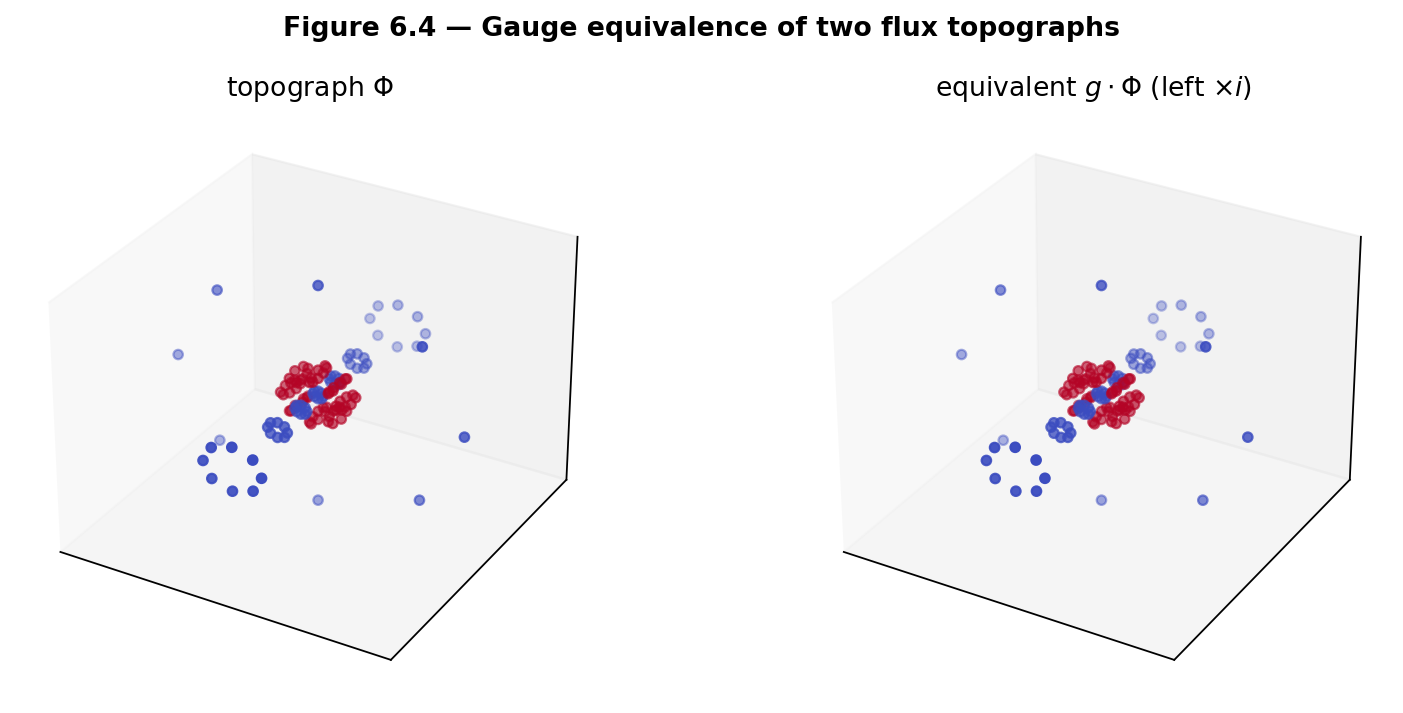
\includegraphics[width=0.92\textwidth,height=0.42\textheight,keepaspectratio]{fig6_4_equivalence.png}
  \caption{Figure 6.4 --- Gauge equivalence of two flux topographs.}
  \label{fig:fig6-4-equivalence}
\end{figure}

\begin{quote}\small\textit{Figure 6.4.* A topograph and its image under left multiplication by \(i\). Value multisets and sorted point clouds match for geometric functionals (\texttt{equivalence\_\allowbreak{}distance} near zero).}\end{quote}

\subsection{Distance and reduced representatives}
\label{ch:ch06_classification:distance-and-reduced-representatives}

\begin{lstlisting}[style=qga]
equivalence_distance(topo_a, topo_b)
reduced_representative(topo)           # minimize value variance in a gauge orbit
enumerate_reduced(topo, dedup_tol=...)  # inequivalent reduced orbit reps
\end{lstlisting}

\textbf{Reduced configurations} are representatives chosen from each approximate equivalence class by a normalization rule (here: minimal value variance among a bounded gauge orbit). The number of distinct reduced configurations is a \textbf{class-number analogue}.

\begin{figure}[htbp]
  \centering
  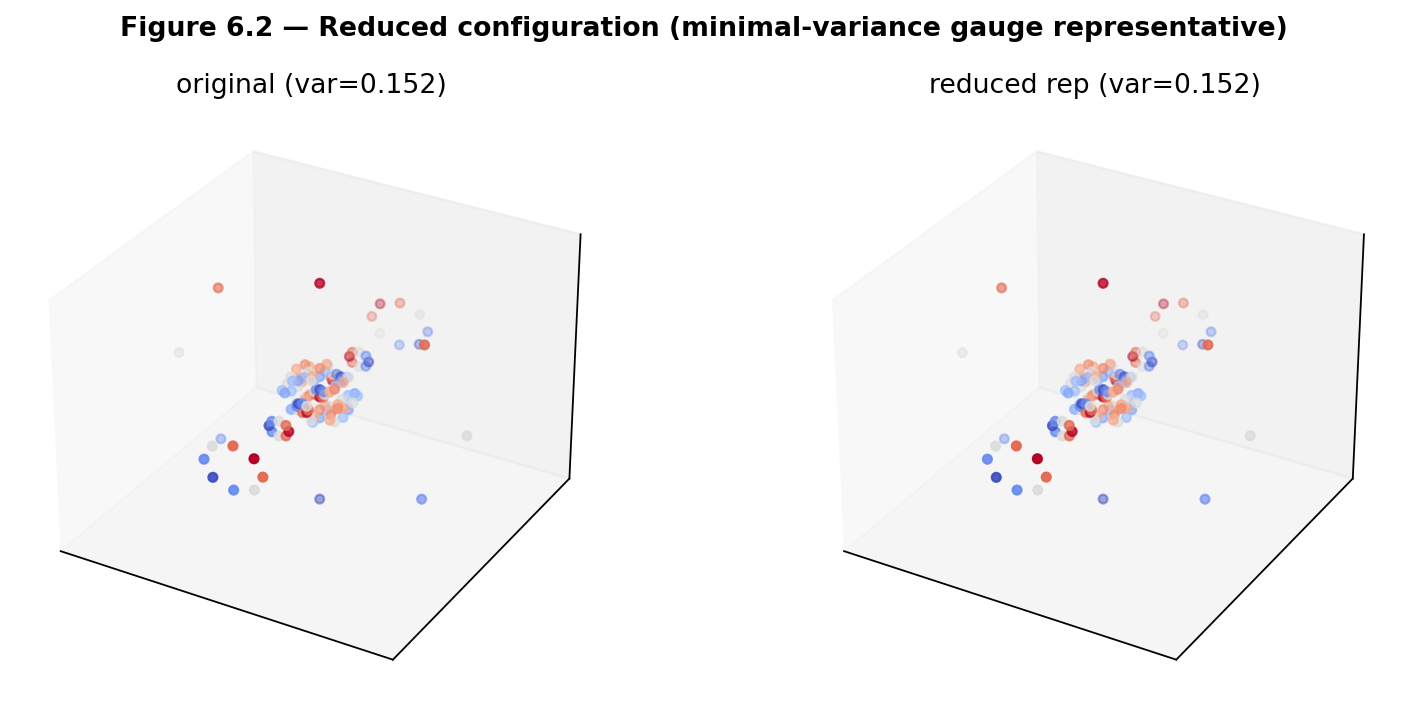
\includegraphics[width=0.92\textwidth,height=0.42\textheight,keepaspectratio]{fig6_2_reduced_config.png}
  \caption{Figure 6.2 --- Reduced configuration.}
  \label{fig:fig6-2-reduced-config}
\end{figure}

\begin{quote}\small\textit{Figure 6.2.* Original topograph vs reduced representative selected by minimal variance under the standard gauge dictionary.}\end{quote}

\bigskip
\noindent\rule{\textwidth}{0.4pt}
\bigskip

\section{6.3 Magic Islands as higher-dimensional class-number phenomena}
\label{ch:ch06_classification:6-3-magic-islands-as-higher-dimensional-class-number-phenome}

\textbf{Magic Islands} are regions in parameter space (or in the space of flux functionals) that contain a high density of reduced configurations with strong periodicity and high stability scores.

They generalize:

\begin{itemize}
\item the finite set of reduced forms for negative discriminant (elliptic case);  
\item the periodic reduced cycles for positive nonsquare discriminant (hyperbolic case).
\end{itemize}

In the Kingdom Come Model, Magic Islands appear as pockets where \texttt{stability\_\allowbreak{}score} is high, \texttt{stability\_\allowbreak{}class} is noble-like, and dynamical simulations show ordered long-term behavior (Ch. 3--5).

\textbf{Invariant discipline (forward pointer).} When classifying topograph types and Magic Islands, keep separate: (i) \emph{algebraic} structure of discrete labels or class-like counts, (ii) \emph{sequential / Model flow} of scores along parameter or \(Z\) sweeps, and (iii) \emph{statistical geometric lock} of a pattern to a continuous base beyond chance. The distinction among these three layers---developed with controls in \textbf{Chapter 9 section 9.5}---applies directly here: high \texttt{stability\_\allowbreak{}score} clusters and visual island order are not automatically the same as an algebraic class number, nor as a proved lock to a continuous geometric coordinate. See also Chapter 10's checklist and \texttt{notes/\allowbreak{}RESEARCH\_\allowbreak{}NOTE\_\allowbreak{}moduli.\allowbreak{}md}.

\begin{figure}[htbp]
  \centering
  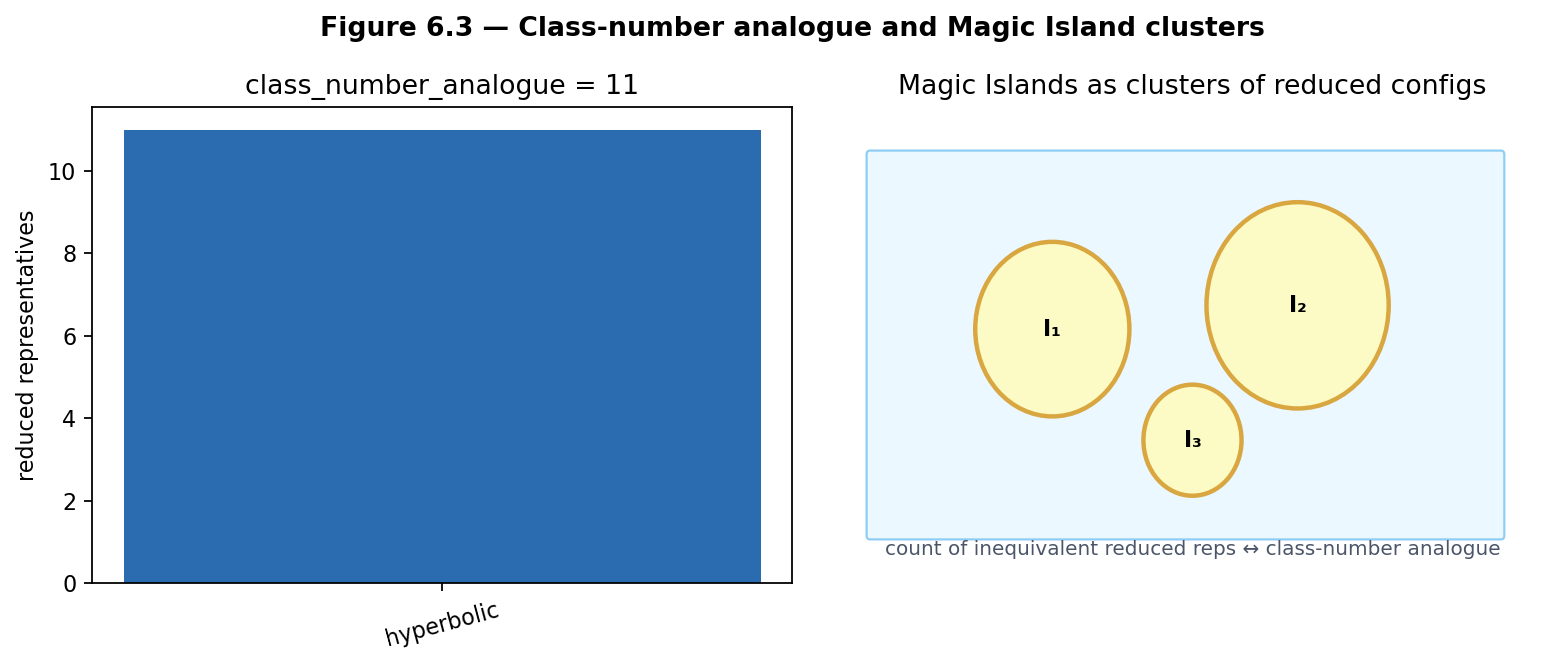
\includegraphics[width=0.92\textwidth,height=0.42\textheight,keepaspectratio]{fig6_3_class_number_analogue.png}
  \caption{Figure 6.3 --- Class-number analogue and Magic Island clusters.}
  \label{fig:fig6-3-class-number-analogue}
\end{figure}

\begin{quote}\small\textit{Figure 6.3.* Left: count of inequivalent reduced representatives by type (\texttt{class\_\allowbreak{}number\_\allowbreak{}analogue}). Right: schematic islands as clusters of reduced configs.}\end{quote}

\begin{figure}[htbp]
  \centering
  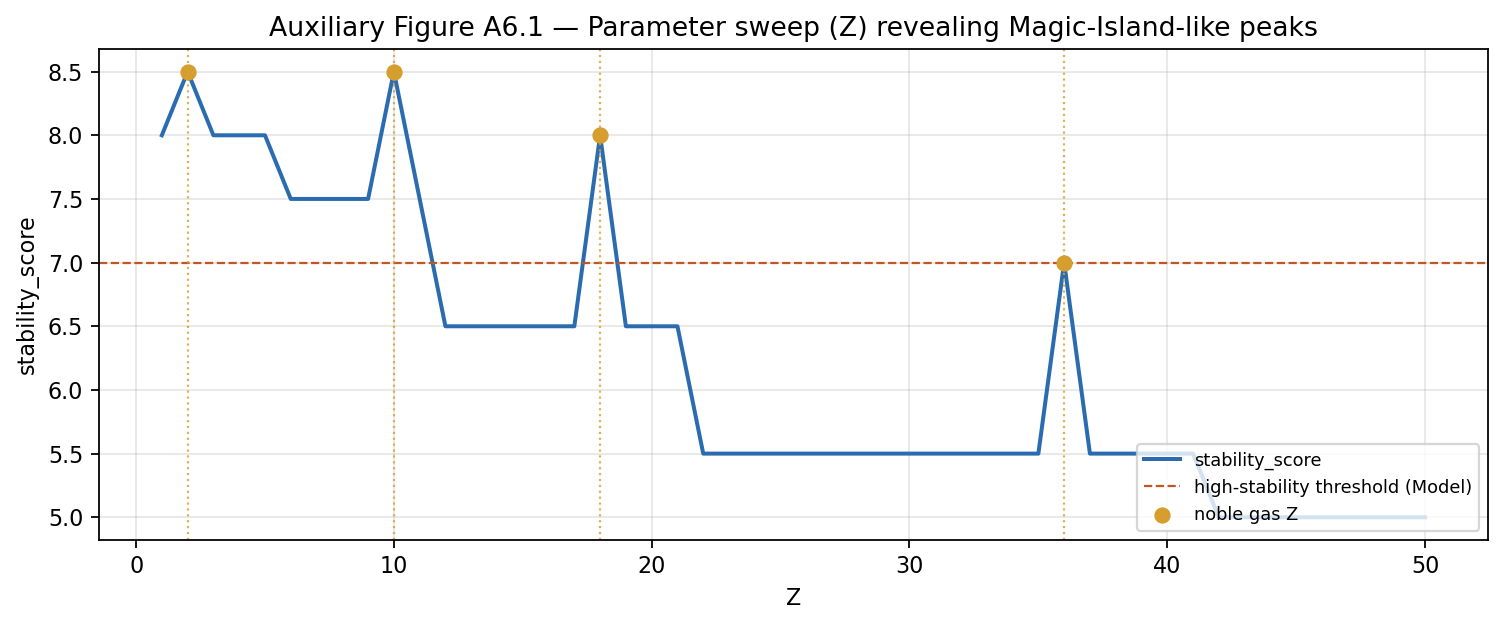
\includegraphics[width=0.92\textwidth,height=0.42\textheight,keepaspectratio]{aux6_1_island_sweep.png}
  \caption{Auxiliary Figure A6.1 --- Z-sweep for island peaks.}
  \label{fig:aux6-1-island-sweep}
\end{figure}

\begin{quote}\small\textit{Auxiliary Figure A6.1.* Portal Model \texttt{stability\_\allowbreak{}score} vs \(Z\) (gold: noble-gas \(Z\); dashed: high-stability threshold). \textbf{Software fact} for the curve; island interpretation remains \textbf{Model}.}\end{quote}

\subsection{Heuristic island score}
\label{ch:ch06_classification:heuristic-island-score}

\begin{lstlisting}[style=qga]
magic_island_score(topo) -> score, period_term, variance_term, separator_term, type
class_number_analogue(topo) -> class_number_analogue, by_type, reduced
\end{lstlisting}

Higher \texttt{magic\_\allowbreak{}island\_\allowbreak{}score} means more ``island-like'' under the pedagogical formula (periodicity + controlled variance + ordered separators). It is \textbf{not} a classical invariant.

\textbf{Open Problem 3 (core of this chapter).} Develop invariants (discriminant analogues, class-number-like counts) that predict the location and size of Magic Islands from lattice data and flux functionals \textbf{without} exhaustive parameter sweeps---and that reduce to classical class numbers under a Hatcher-style restriction.

See \texttt{notes/\allowbreak{}open\_\allowbreak{}problems.\allowbreak{}md}. Depends on OP1 (adjacency) and OP2 (topograph axioms).

\bigskip
\noindent\rule{\textwidth}{0.4pt}
\bigskip

\section{6.4 First computational labs}
\label{ch:ch06_classification:6-4-first-computational-labs}

Helpers: \texttt{lib/\allowbreak{}flux\_\allowbreak{}topograph.\allowbreak{}py} \(\cdot\) \textbf{Appendix C ?C.3}.

\begin{itemize}
\item \textbf{6.A} \texttt{classify\_\allowbreak{}topograph\_\allowbreak{}type}.
\item \textbf{6.B} \texttt{enumerate\_\allowbreak{}reduced} / \texttt{class\_\allowbreak{}number\_\allowbreak{}analogue} (use modest lattices).
\item \textbf{6.C} Portal \texttt{stability\_\allowbreak{}score} vs \(Z\) (no \texttt{magic\_\allowbreak{}flag}).
\item \textbf{6.D} \texttt{equivalence\_\allowbreak{}distance} after left multiplication.
\end{itemize}

\begin{lstlisting}[style=qga,language=python]
from lib.flux_topograph import classify_topograph_type, class_number_analogue
# build topo as in Appendix C ?C.3
# print(classify_topograph_type(topo)["type"])
\end{lstlisting}

\bigskip
\noindent\rule{\textwidth}{0.4pt}
\bigskip

\section{Exercises}
\label{ch:ch06_classification:exercises}

\textbf{6.A (hand).} State the four classical types of quadratic forms/topographs in Hatcher and map each to the lifted types in this chapter.

\textbf{6.B (hand).} Explain why reduced configurations are useful for classification (one paragraph).

\textbf{6.C (code).} Complete Labs 6.A--6.B. Report the type and number of reduced representatives for your topograph.

\textbf{6.D (code).} Run Lab 6.C for \(Z=1\) to \(50\). Tabulate \texttt{stability\_\allowbreak{}score} and mark noble-gas \(Z\). Identify any visible Magic-Island-like clusters.

\textbf{6.E (visual).} Generate two equivalent topographs (via gauge action) and confirm \texttt{equivalence\_\allowbreak{}distance} is small; compare separator counts.

\textbf{6.F (Hatcher bridge).} In Hatcher, the class number counts inequivalent reduced forms for a given discriminant. Sketch how a ``Magic Island count'' / \texttt{class\_\allowbreak{}number\_\allowbreak{}analogue} could play an analogous role here.

\textbf{6.G (Open Problem 3 teaser).} Using \texttt{enumerate\_\allowbreak{}reduced} and \texttt{magic\_\allowbreak{}island\_\allowbreak{}score}, test whether the current candidate adjacency produces consistent island scores across small changes in functional (\texttt{hopf\_\allowbreak{}height} vs \texttt{hopf\_\allowbreak{}y1}). Document inconsistencies---they constrain OP3 invariants.

\textbf{6.H (forward).} Why will the ideal-class-group lift in Chapter 8 depend on the classification developed here?

\textbf{6.I (software honesty).} In one paragraph, distinguish: (i) heuristic \texttt{classify\_\allowbreak{}topograph\_\allowbreak{}type}, (ii) portal \texttt{stability\_\allowbreak{}score} vs \(Z\), (iii) classical class numbers. Assign claim types.

\bigskip
\noindent\rule{\textwidth}{0.4pt}
\bigskip

\section{Code and asset pointers}
\label{ch:ch06_classification:code-and-asset-pointers}

\begin{lstlisting}[style=qga]
qga/lib/flux_topograph.py   # Ch. 5-6 helpers
qga/lib/hopf_lattice.py
kingdom.core.flux_flywheel
kingdom.viz.magic_island
\end{lstlisting}

\textbf{Figures:} \texttt{scripts/\allowbreak{}generate\_\allowbreak{}ch6\_\allowbreak{}figures.\allowbreak{}py} \textbf{Related portal:} Flux Flywheel tab; Magic Island heatmap. \textbf{Open problems:} OP3 (this chapter); OP2 (topograph axioms); OP1 (adjacency).

\bigskip
\noindent\rule{\textwidth}{0.4pt}
\bigskip

\section{Looking ahead}
\label{ch:ch06_classification:looking-ahead}

We now have a working \textbf{Model} classification of flux topographs, reduced configurations, and Magic Islands---the quaternionic narrative lift of Hatcher's classification theory. In \textbf{Chapter 7} we connect these classified objects to the \(Z\mapsto\) flywheel map, turning arithmetic-looking invariants into a periodic-table proxy. \textbf{Chapter 8} will then lift the class group itself to the quaternionic / Hopf setting. \textbf{Chapter 9 section 9.5} will sharpen the arithmetic--geometry boundary with a controlled three-layer analysis (algebra / sequential flow / angle lock) that you can already apply when reading island plots in this chapter.

With classification in hand, we are ready to bridge number theory and the emergent physics of the Kingdom Come Model.

\bigskip
\noindent\rule{\textwidth}{0.4pt}
\bigskip



% Auto-generated from book/07_representations_z_flux.md — do not edit by hand
% Regenerated by scripts/md_to_latex.py

\chapter{The \(Z \mapsto\) Flux Map and Representation Theory}
\label{ch:ch07_z_map}

This chapter connects the classified flux topographs and Magic Islands of Chapters 5--6 to the atomic number \(Z\). We define the \textbf{\(Z \mapsto\) flux map}, interpret it as a representation-theoretic bridge (which ``numbers'' are represented by stable flux configurations), and examine how Magic Islands align with chemically and physically special elements. The construction remains a \textbf{Model} with explicit validation pathways (Chapter 10).

\textbf{Learning goals}

\begin{enumerate}
\item Define the \(Z \mapsto\) flywheel / flux configuration map formally.  
\item Interpret the map as representation theory on the gauged Hopf lattice.  
\item Connect Magic Islands to the periodic table and noble-gas stability.  
\item Examine chemical and physical proxies (stability scores, shell descriptors, extended fields).  
\item Prepare the bridge to class-group ideas (Chapter 8) and observational validation (Chapter 10).
\end{enumerate}

\textbf{Figures in this chapter}

\begin{center}
\small
\setlength{\tabcolsep}{4pt}
\begin{tabularx}{\textwidth}{@{}>{\raggedright\arraybackslash}p{0.12\textwidth}>{\raggedright\arraybackslash}X>{\raggedright\arraybackslash}X@{}}
\toprule
Tag & File & Role \\
\midrule
Fig. 7.1 & \texttt{figures/\allowbreak{}fig7\_\allowbreak{}1\_\allowbreak{}z\_\allowbreak{}to\_\allowbreak{}flywheel.\allowbreak{}png} & Schematic of the \(Z \mapsto\) flux map \\
Fig. 7.2 & \texttt{figures/\allowbreak{}fig7\_\allowbreak{}2\_\allowbreak{}magic\_\allowbreak{}island\_\allowbreak{}periodic\_\allowbreak{}table.\allowbreak{}png} & Magic Island scores on a schematic table \\
Fig. 7.3 & \texttt{figures/\allowbreak{}fig7\_\allowbreak{}3\_\allowbreak{}stability\_\allowbreak{}vs\_\allowbreak{}z.\allowbreak{}png} & \texttt{stability\_\allowbreak{}score} vs \(Z\) (portal data) \\
Fig. 7.4 & \texttt{figures/\allowbreak{}fig7\_\allowbreak{}4\_\allowbreak{}electron\_\allowbreak{}cloud\_\allowbreak{}flux.\allowbreak{}png} & Electron cloud as flux distribution \\
Aux A7.1 & \texttt{figures/\allowbreak{}aux7\_\allowbreak{}1\_\allowbreak{}he\_\allowbreak{}fe\_\allowbreak{}au\_\allowbreak{}stills.\allowbreak{}png} & He, Fe, Au flywheel stills \\
\bottomrule
\end{tabularx}
\end{center}


\textbf{Claim discipline}

\begin{center}
\small
\setlength{\tabcolsep}{4pt}
\begin{tabularx}{\textwidth}{@{}>{\raggedright\arraybackslash}p{0.70\textwidth}>{\raggedright\arraybackslash}X@{}}
\toprule
Claim & Type \\
\midrule
Four-square theorem and classical representation by norms (Ch. 1) & \textbf{Theorem} \\
Existence and implementation of the coded \(Z \mapsto\) map & \textbf{Software fact} \\
Map as representation theory; Magic Islands as periodic-table proxy; physical emergence & \textbf{Model} \\
Any claim that topology \emph{derives} real chemistry as a law of nature & \textbf{Hypothesis} (Ch. 10 validation) \\
\texttt{map\_\allowbreak{}z\_\allowbreak{}to\_\allowbreak{}flywheel[\_\allowbreak{}extended]} metrics & \textbf{Software fact} \\
\bottomrule
\end{tabularx}
\end{center}


\bigskip
\noindent\rule{\textwidth}{0.4pt}
\bigskip

\section{The \(Z \mapsto\) flux map}
\label{ch:ch07_z_map:the-z-mapsto-flux-map}

The Kingdom Come portal implements a function that takes an atomic number \(Z\) and returns a flywheel configuration together with stability and chemistry-facing metrics:

\begin{align*}
Z \longmapsto \bigl(&
  \text{flywheel / detuning state},\\
  &\texttt{stability\_score},\;
  \texttt{stability\_class},\\
  &\texttt{is\_noble\_gas},\;\ldots
\bigr).
\end{align*}

\textbf{Primary entry points}

\begin{center}
\small
\setlength{\tabcolsep}{4pt}
\begin{tabularx}{\textwidth}{@{}>{\raggedright\arraybackslash}X>{\raggedright\arraybackslash}X@{}}
\toprule
Function & Role \\
\midrule
\texttt{map\_\allowbreak{}z\_\allowbreak{}to\_\allowbreak{}flywheel(z)} & Core map: detuning, gauge params, \texttt{stability\_\allowbreak{}score}, class labels \\
\texttt{map\_\allowbreak{}z\_\allowbreak{}to\_\allowbreak{}flywheel\_\allowbreak{}extended(z)} & Adds alignment, IE proxies, magnetic-moment validation fields \\
\bottomrule
\end{tabularx}
\end{center}


There is still \textbf{no} \texttt{magic\_\allowbreak{}flag} key. Treat high \texttt{stability\_\allowbreak{}score}, noble-gas class strings, and \texttt{is\_\allowbreak{}noble\_\allowbreak{}gas=True} as the Model's island indicators.

The map is built on the gauged Hopf lattice and flux-topograph language of previous chapters. Different detuning parameters select different stability islands; a documented ultra-stable lock (Magic Island Sweep reference in portal notes) serves as a noble-gas-like template.

\begin{figure}[htbp]
  \centering
  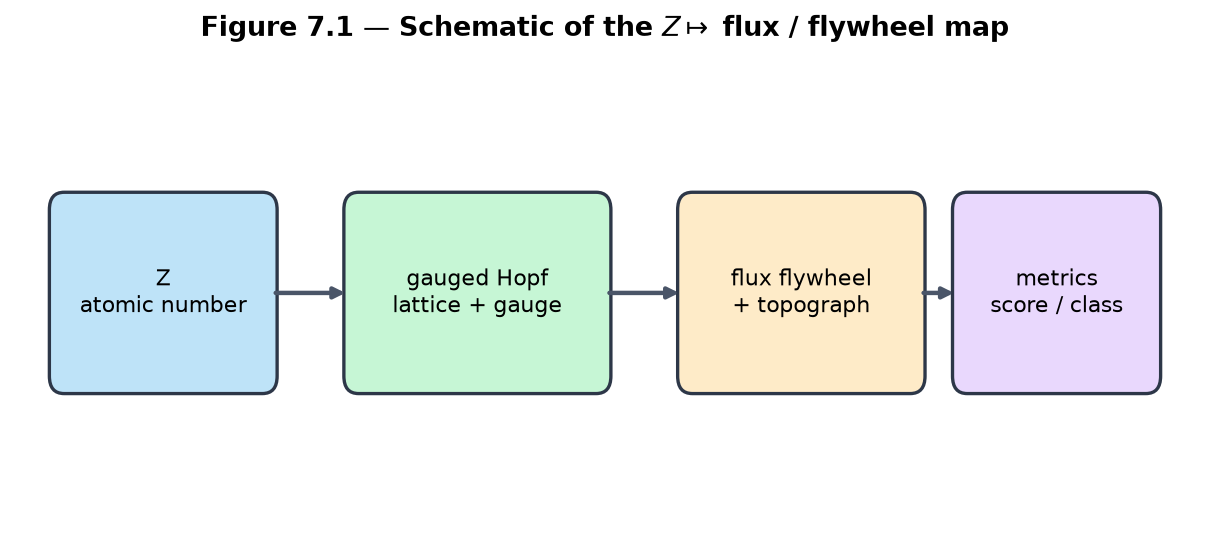
\includegraphics[width=0.92\textwidth,height=0.42\textheight,keepaspectratio]{fig7_1_z_to_flywheel.png}
  \caption{Pipeline: atomic number \(\rightarrow\) lattice / gauge data \(\rightarrow\) flux flywheel + topograph \(\rightarrow\) scored metrics.}
  \label{fig:fig7-1-z-to-flywheel}
\end{figure}

\textbf{Claim type.} Reproducible coded map: \textbf{Software fact}. Interpreting outputs as \emph{the} emergence mechanism of the periodic table: \textbf{Model}.

\subsection{Book helper}
\label{ch:ch07_z_map:book-helper}

\begin{lstlisting}[style=qga]
stability_landscape_z(z_values=...)          # list of dict rows
stability_landscape_z(z_range=(1, 50))       # inclusive range
stability_landscape_z(z_range=(1, 30), extended=True)
\end{lstlisting}

\bigskip
\noindent\rule{\textwidth}{0.4pt}
\bigskip

\section{Representation theory on the gauged Hopf lattice}
\label{ch:ch07_z_map:representation-theory-on-the-gauged-hopf-lattice}

In classical number theory, representation by quadratic forms asks which integers \(n\) satisfy \(f(x,y)=n\) for a given form (Hatcher Chapter 6). Quaternion norms answer which \(n\) are sums of four squares (Chapter 1, \textbf{Theorem}).

Here we ask an analogous \textbf{Model} question:

> Which atomic numbers \(Z\) are ``represented'' by stable flux configurations on the gauged Hopf lattice?

Stable flywheels correspond to reduced configurations with high \texttt{magic\_\allowbreak{}island\_\allowbreak{}score} (Chapter 6) and high portal \texttt{stability\_\allowbreak{}score}. The map therefore selects, for each \(Z\), a configuration (or orbit) intended to match observed chemical/nuclear specialness.

\begin{center}
\small
\setlength{\tabcolsep}{4pt}
\begin{tabularx}{\textwidth}{@{}>{\raggedright\arraybackslash}X>{\raggedright\arraybackslash}X@{}}
\toprule
Classical & Quaternionic / Hopf Model \\
\midrule
Form \(f\) & Lattice + gauge group + flux functional \\
Represented integer \(n\) & Atomic number \(Z\) (and related quantum numbers) \\
Class / genus of forms & Equivalence class of topographs / flywheels \\
Class number & \texttt{class\_\allowbreak{}number\_\allowbreak{}analogue} / island counts (Ch. 6) \\
\bottomrule
\end{tabularx}
\end{center}


This is a \textbf{representation-theoretic reading}, not a theorem that every chemical property is a lattice invariant.

\begin{figure}[htbp]
  \centering
  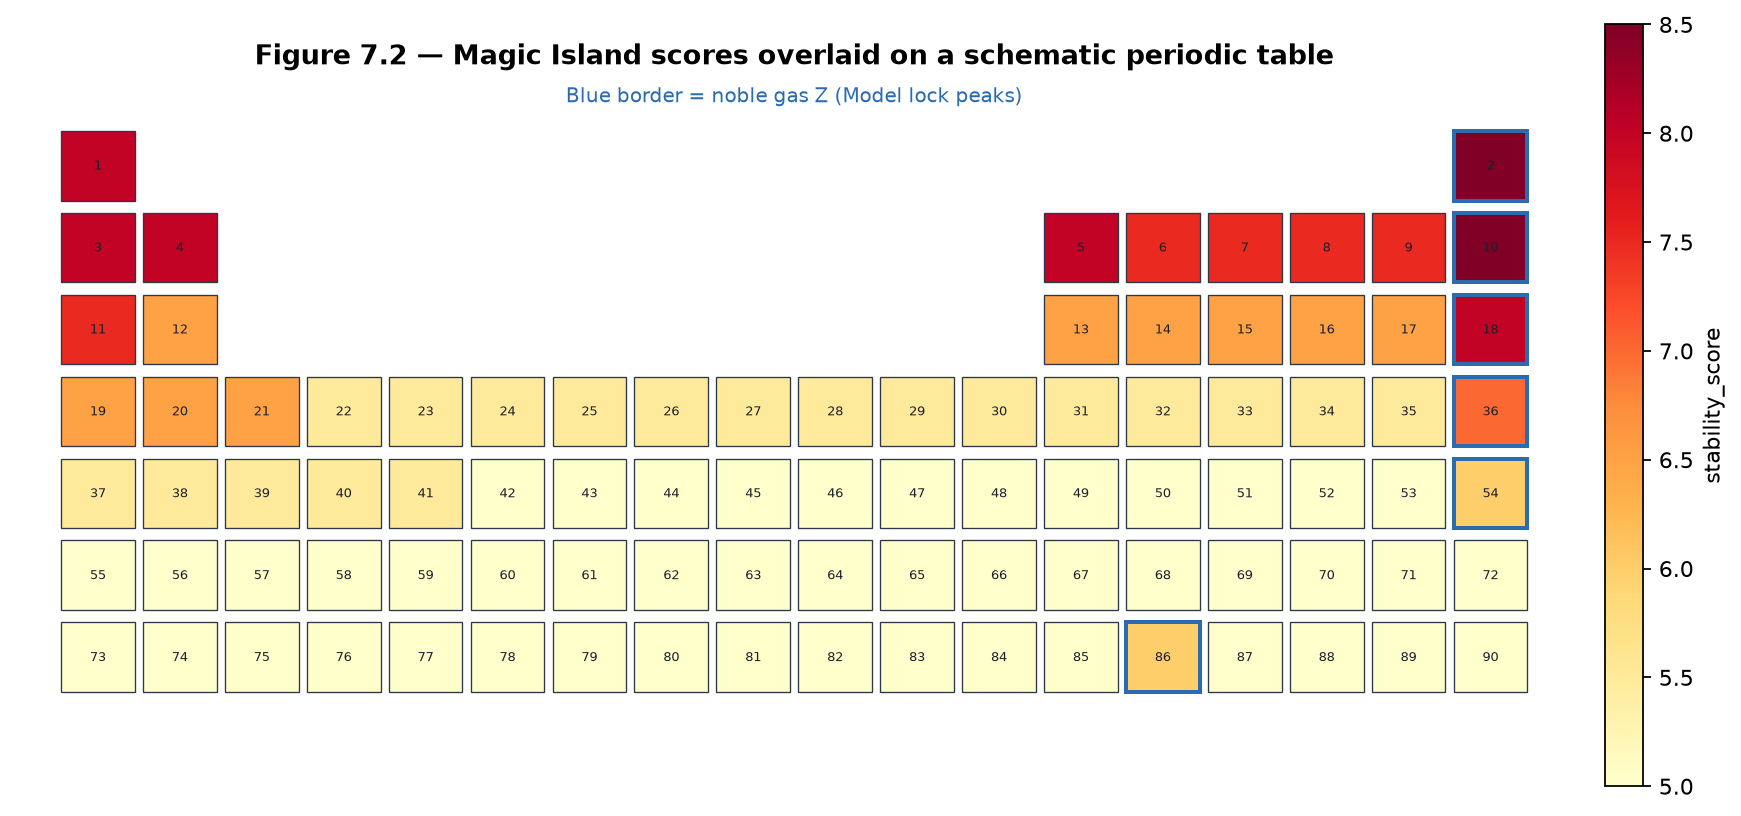
\includegraphics[width=0.92\textwidth,height=0.42\textheight,keepaspectratio]{fig7_2_magic_island_periodic_table.png}
  \caption{Cells colored by portal \texttt{stability\_\allowbreak{}score}; blue borders mark noble-gas \(Z\). Layout is a simplified table for visualization (f-block truncated)---software + Model.}
  \label{fig:fig7-2-magic-island-periodic-table}
\end{figure}

\bigskip
\noindent\rule{\textwidth}{0.4pt}
\bigskip

\section{Chemistry-facing scores (Hypothesis --- developed in Part V)}
\label{ch:ch07_z_map:chemistry-facing-scores-hypothesis-developed-in-part-v}

Magic Islands as \emph{chemical} stability, noble-gas locks, and ionization-energy alignment are \textbf{not} theorems of Part III. They are Hypothesis H2 / H3, with Table T4 protocols and an H2 ablation (noble-gas bonuses off) in \textbf{Chapter 10} and Appendix D. This section keeps only a pointer so the \(Z\mapsto\) map can be used as a \textbf{Model} representation without promoting chemistry.

Figure 7.3 is a portal software curve, not a finding.

\begin{figure}[htbp]
  \centering
  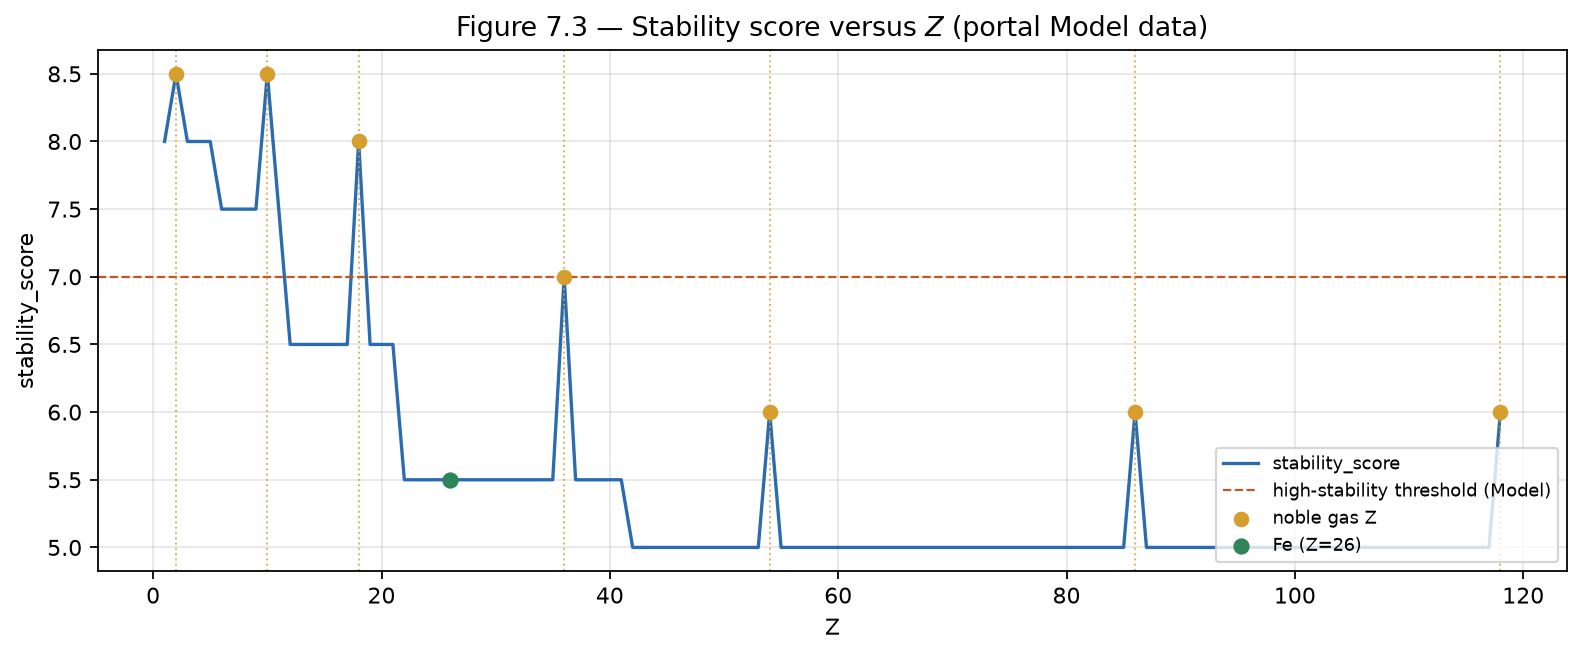
\includegraphics[width=0.92\textwidth,height=0.42\textheight,keepaspectratio]{fig7_3_stability_vs_z.png}
  \caption{Portal \texttt{stability\_\allowbreak{}score} vs atomic number. Gold: noble-gas \(Z\) (explicit bonuses live in the portal map). Interpretation: \textbf{Hypothesis}, Part V. Lab 7 must ablate those bonuses before any alignment claim.}
  \label{fig:fig7-3-stability-vs-z}
\end{figure}

\textbf{Open Problem 4 (shared with Ch. 10).} Up to gauge, is the map \(Z\mapsto\) flywheel configuration unique under stated axioms? See \texttt{notes/\allowbreak{}open\_\allowbreak{}problems.\allowbreak{}md}.

\bigskip
\noindent\rule{\textwidth}{0.4pt}
\bigskip

\section{Electron-cloud visuals (Software fact --- Part V)}
\label{ch:ch07_z_map:electron-cloud-visuals-software-fact-part-v}

Portal electron-cloud pictures (\texttt{kingdom.\allowbreak{}viz.\allowbreak{}electron\_\allowbreak{}cloud}) are \textbf{Software facts} about the renderer, not Schrödinger solutions and not a Part III theorem. Chemistry-facing reading: \textbf{Part V}.

\begin{figure}[htbp]
  \centering
  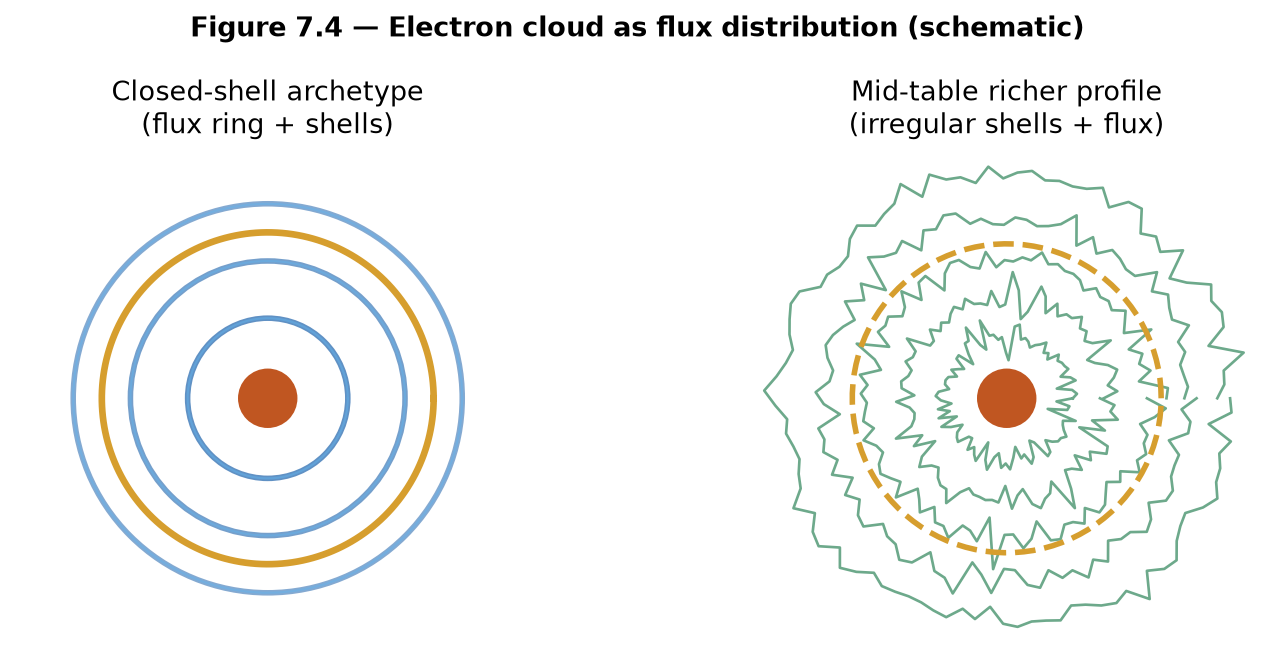
\includegraphics[width=0.92\textwidth,height=0.42\textheight,keepaspectratio]{fig7_4_electron_cloud_flux.png}
  \caption{Schematic closed-shell vs mid-table flux-derived profiles (portal style).}
  \label{fig:fig7-4-electron-cloud-flux}
\end{figure}

\begin{figure}[htbp]
  \centering
  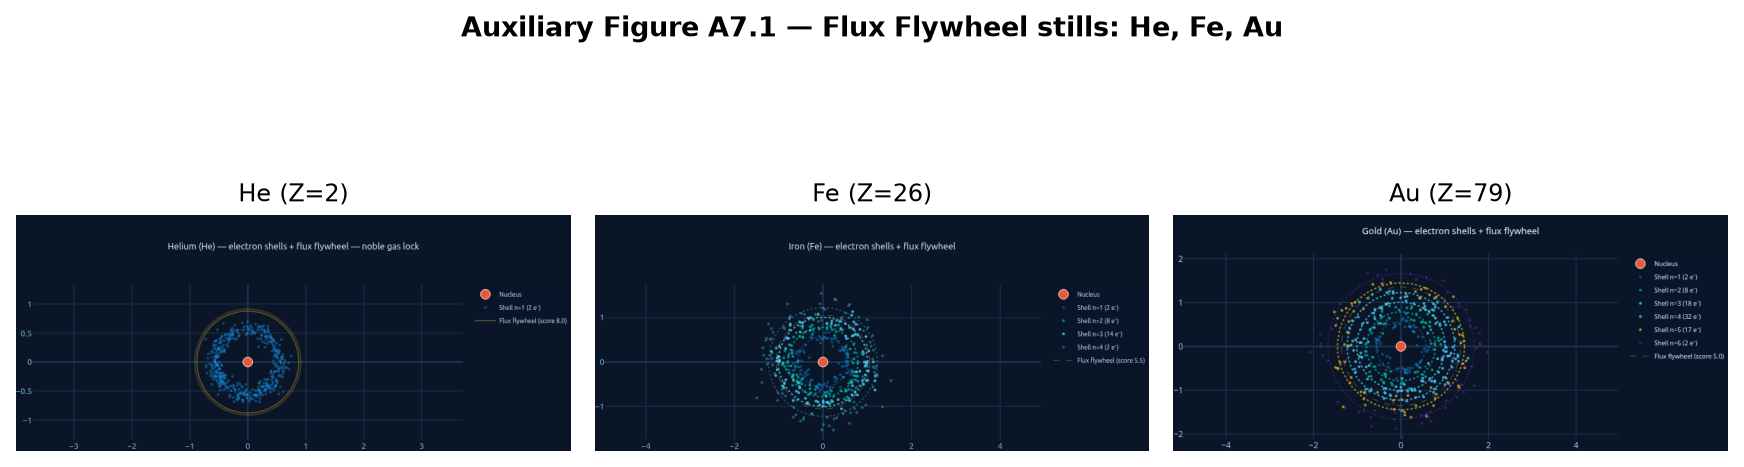
\includegraphics[width=0.92\textwidth,height=0.42\textheight,keepaspectratio]{aux7_1_he_fe_au_stills.png}
  \caption{Portal Flux Flywheel stills: He (\(Z=2\)), Fe (\(Z=26\)), Au (\(Z=79\)). Sources: \texttt{kingdom/\allowbreak{}z\_\allowbreak{}knowns/\allowbreak{}frame\_\allowbreak{}0002.\allowbreak{}png}, \texttt{frame\_\allowbreak{}0026.\allowbreak{}png}, \texttt{frame\_\allowbreak{}0079.\allowbreak{}png}.}
  \label{fig:aux7-1-he-fe-au-stills}
\end{figure}

\bigskip
\noindent\rule{\textwidth}{0.4pt}
\bigskip

\section{First computational labs}
\label{ch:ch07_z_map:first-computational-labs}

Portal: \texttt{map\_\allowbreak{}z\_\allowbreak{}to\_\allowbreak{}flywheel[\_\allowbreak{}extended]} \(\cdot\) \texttt{stability\_\allowbreak{}landscape\_\allowbreak{}z} \(\cdot\) \textbf{Appendix C \S{}C.3}.

\begin{itemize}
\item \textbf{7.A} Scores for \(Z\in\{2,10,26,79,118\}\).
\item \textbf{7.B} \texttt{stability\_\allowbreak{}landscape\_\allowbreak{}z(z\_\allowbreak{}range=(1,50))} high islands.
\item \textbf{7.C} Noble vs neighbors (\(Z=10,11,12\)).
\item \textbf{7.D} Gradio Flux Flywheel / Aux A7.1.
\item \textbf{7.E} Extended fields He vs Fe.
\end{itemize}

\begin{lstlisting}[style=qga,language=python]
from kingdom.core.flux_flywheel import map_z_to_flywheel
print(map_z_to_flywheel(2)["stability_score"], map_z_to_flywheel(2).get("is_noble_gas"))
\end{lstlisting}

\bigskip
\noindent\rule{\textwidth}{0.4pt}
\bigskip

\section{Exercises}
\label{ch:ch07_z_map:exercises}

\textbf{7.A (hand).} In one paragraph, explain why the \(Z\mapsto\) map can be viewed as a representation problem on the gauged Hopf lattice.

\textbf{7.B (hand).} Why might Magic Islands near noble-gas \(Z\) be especially stable in the Model? Connect to closed-shell ideas and Chapter 6 reduced configurations.

\textbf{7.C (code).} Complete Labs 7.A--7.B. Tabulate \texttt{stability\_\allowbreak{}score} and \texttt{is\_\allowbreak{}noble\_\allowbreak{}gas} for \(Z=1\) to \(30\). Identify the strongest islands.

\textbf{7.D (code).} Complete Lab 7.E for \(Z=2\) and \(Z=26\). What differences appear in extended fields?

\textbf{7.E (visual).} Render or inspect flux-derived clouds for He and Fe. Describe how Model geometry differs between a closed-shell case and a mid-table case.

\textbf{7.F (Hatcher bridge).} In Hatcher Chapter 6, representation by quadratic forms uses genus, characters, and quadratic reciprocity. Sketch how the \(Z\mapsto\) map might eventually use ``genus'' of flux configurations or topological characters on the lattice.

\textbf{7.G (forward).} Why will class-group ideas (Chapter 8) be relevant to which \(Z\) land in Magic Islands?

\textbf{7.H (software honesty).} Distinguish in one paragraph: (i) the coded \(Z\mapsto\) map as software, (ii) its use as a periodic-table proxy (\textbf{Model}), (iii) any claim that it derives real chemistry from topology (\textbf{Hypothesis}).

\textbf{7.I (Open Problem 4 teaser).} Fix a small set of gauge sequences from Chapter 4. For two nearby \(Z\), inspect whether flywheel metrics could plausibly share an orbit. What would count as non-uniqueness of the map?

\bigskip
\noindent\rule{\textwidth}{0.4pt}
\bigskip

\section{Code and asset pointers}
\label{ch:ch07_z_map:code-and-asset-pointers}

\begin{lstlisting}[style=qga]
kingdom.core.flux_flywheel.map_z_to_flywheel[_extended]
qga/lib/flux_topograph.stability_landscape_z
kingdom.viz.magic_island.build_magic_island_heatmap
kingdom.viz.electron_cloud.build_electron_cloud_figure
kingdom/z_knowns/frame_XXXX.png   # flywheel stills
\end{lstlisting}

\textbf{Figures:} \texttt{scripts/\allowbreak{}generate\_\allowbreak{}ch7\_\allowbreak{}figures.\allowbreak{}py} \textbf{Related portal:} Flux Flywheel tab (interactive \(Z\) slider). \textbf{Open problems:} OP4 (uniqueness); OP3 (island invariants); OP5 (\(350/\pi\), Ch. 10).

\bigskip
\noindent\rule{\textwidth}{0.4pt}
\bigskip

\section{Looking ahead}
\label{ch:ch07_z_map:looking-ahead}

The \(Z\mapsto\) flux map links the classified arithmetic objects of Chapters 5--6 to concrete atomic numbers. In \textbf{Chapter 8} we lift the class group itself to the quaternionic / Hopf setting, giving a deeper arithmetic home for Magic Island counts and equivalence classes. \textbf{Chapter 10} returns to observational validation of the whole construction---including statistical protocols for the \(350/\pi\) signature and \(Z\)-map correlations.

With the representation bridge in place, we are ready for the ideal-class-group lift.

\bigskip
\noindent\rule{\textwidth}{0.4pt}
\bigskip



\part{Arithmetic Depth}
% Auto-generated from book/08_class_group.md — do not edit by hand
% Regenerated by scripts/md_to_latex.py

\chapter{Chapter 8 --- Composition and Class Groups in the Quaternionic Setting}
\label{ch:ch08_class_group}

This chapter lifts Gauss composition of binary quadratic forms and the ideal class group (Hatcher Chapters 7--8) to the gauged Hopf lattice and quaternion orders. We define composition of flux configurations / flywheels, construct class-group analogues, and examine how these structures organize Magic Islands and equivalence classes. The theory remains a \textbf{Model} construction, with \textbf{Open Problem 6} as its central open edge.

\textbf{Learning goals}

\begin{enumerate}
\item Recall Gauss composition of quadratic forms and its arithmetic meaning.  
\item Lift composition to flux configurations and flywheels on the gauged Hopf lattice.  
\item Construct class-group analogues for flux topographs (and, later, quaternion orders).  
\item Connect class-group structure to Magic Island counts and equivalence classes.  
\item Prepare the ground for quaternion algebras and ideal theory (Chapter 9).
\end{enumerate}

\textbf{Figures in this chapter}

\begin{center}
\small
\begin{tabular}{@{}lp{0.28\textwidth}p{0.28\textwidth}@{}}
\toprule
Tag & File & Role \\
\midrule
Fig. 8.1 & \texttt{figures/fig8\_1\_gauss\_composition.png} & Classical Gauss composition diagram \\
Fig. 8.2 & \texttt{figures/fig8\_2\_flywheel\_composition.png} & Composition of two flux topographs \\
Fig. 8.3 & \texttt{figures/fig8\_3\_class\_group\_analogue.png} & Class-group analogue on the lattice \\
Fig. 8.4 & \texttt{figures/fig8\_4\_island\_from\_class.png} & Magic Island from class-group data \\
Aux A8.1 & \texttt{figures/aux8\_1\_composition\_table.png} & Small composition table \\
\bottomrule
\end{tabular}
\end{center}


\textbf{Claim discipline}

\begin{center}
\small
\begin{tabular}{@{}lp{0.55\textwidth}@{}}
\toprule
Claim & Type \\
\midrule
Classical Gauss composition and ideal class groups (Hatcher Ch. 7--8) & \textbf{Theorem} (cited) \\
Composition of flux configurations / flywheels; class-group analogues & \textbf{Model} (core of OP6) \\
\texttt{qga/lib/composition.py} helpers & \textbf{Software fact} \\
\bottomrule
\end{tabular}
\end{center}


\bigskip
\noindent\rule{\textwidth}{0.4pt}
\bigskip

\section{8.1 Gauss composition --- classical reminder}
\label{ch:ch08_class_group:8-1-gauss-composition-classical-reminder}

In Hatcher Chapter 7, Gauss defined a composition law on (primitive) binary quadratic forms of the same discriminant. Up to equivalence, the law is associative and turns the set of classes into a finite abelian group---the \textbf{class group} of the discriminant. The same group appears as the ideal class group of the corresponding quadratic order (Hatcher Chapter 8).

\begin{figure}[htbp]
  \centering
  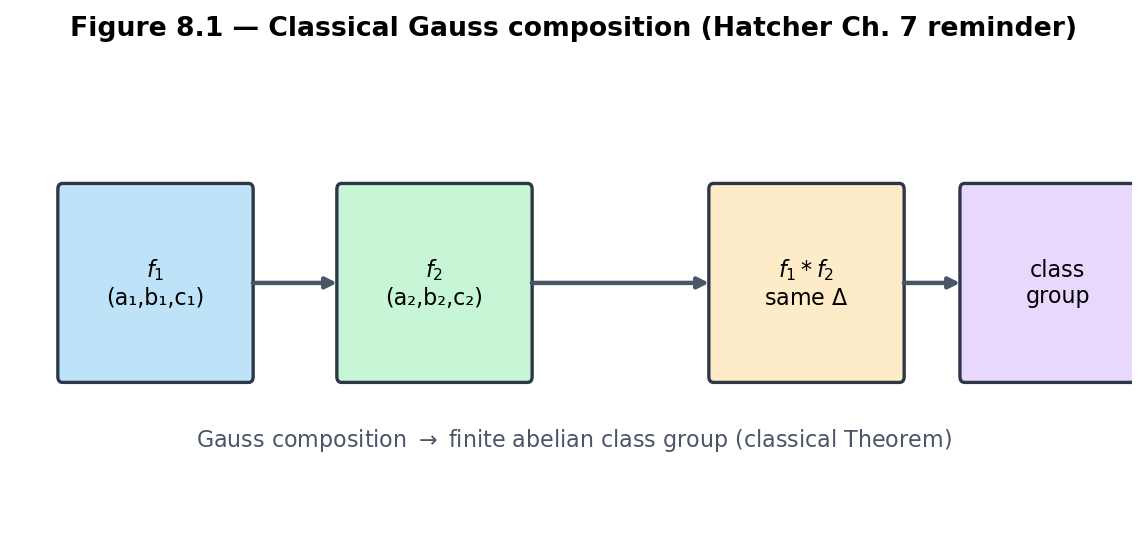
\includegraphics[width=0.92\textwidth,height=0.42\textheight,keepaspectratio]{fig8_1_gauss_composition.png}
  \caption{Figure 8.1 --- Classical Gauss composition.}
  \label{fig:fig8-1-gauss-composition}
\end{figure}

\begin{quote}\small\textit{Figure 8.1.* Forms \(f_1,f_2\) of fixed discriminant compose to a third form; classes form a finite abelian group. This is classical \textbf{Theorem} territory; we cite Hatcher / Gauss rather than re-prove.}\end{quote}

Why it matters here: class groups encode failure of unique factorization and control representation theory---exactly the arithmetic depth we want to lift for Magic Islands and the \(Z\mapsto\) map.

\bigskip
\noindent\rule{\textwidth}{0.4pt}
\bigskip

\section{8.2 Lifting composition to flux configurations and flywheels}
\label{ch:ch08_class_group:8-2-lifting-composition-to-flux-configurations-and-flywheels}

On the gauged Hopf lattice we define a \textbf{composition} of two flux topographs (or flywheels) by combining values and/or points, then reducing with the Chapter 6 normalization.

\subsection{Candidate methods (\textbf{Model})}
\label{ch:ch08_class_group:candidate-methods-model}

\begin{center}
\small
\begin{tabular}{@{}lp{0.55\textwidth}@{}}
\toprule
Method (code) & Rule \\
\midrule
\texttt{value\_sum} & Pointwise average of values; averaged then renormed points \\
\texttt{value\_product} & Pointwise product (scaled) \\
\texttt{value\_bilinear} & Soft bilinear blend \((V_a+V_b+V_a V_b)/3\) \\
\texttt{point\_mult} & Quaternion multiply corresponding lattice points; recompute functional \\
\bottomrule
\end{tabular}
\end{center}


\begin{lstlisting}[style=qga]
compose_flywheels(topo_a, topo_b, method="value_sum")
reduce_composition(composed) -> topograph, classification, magic_island_score
\end{lstlisting}

\begin{figure}[htbp]
  \centering
  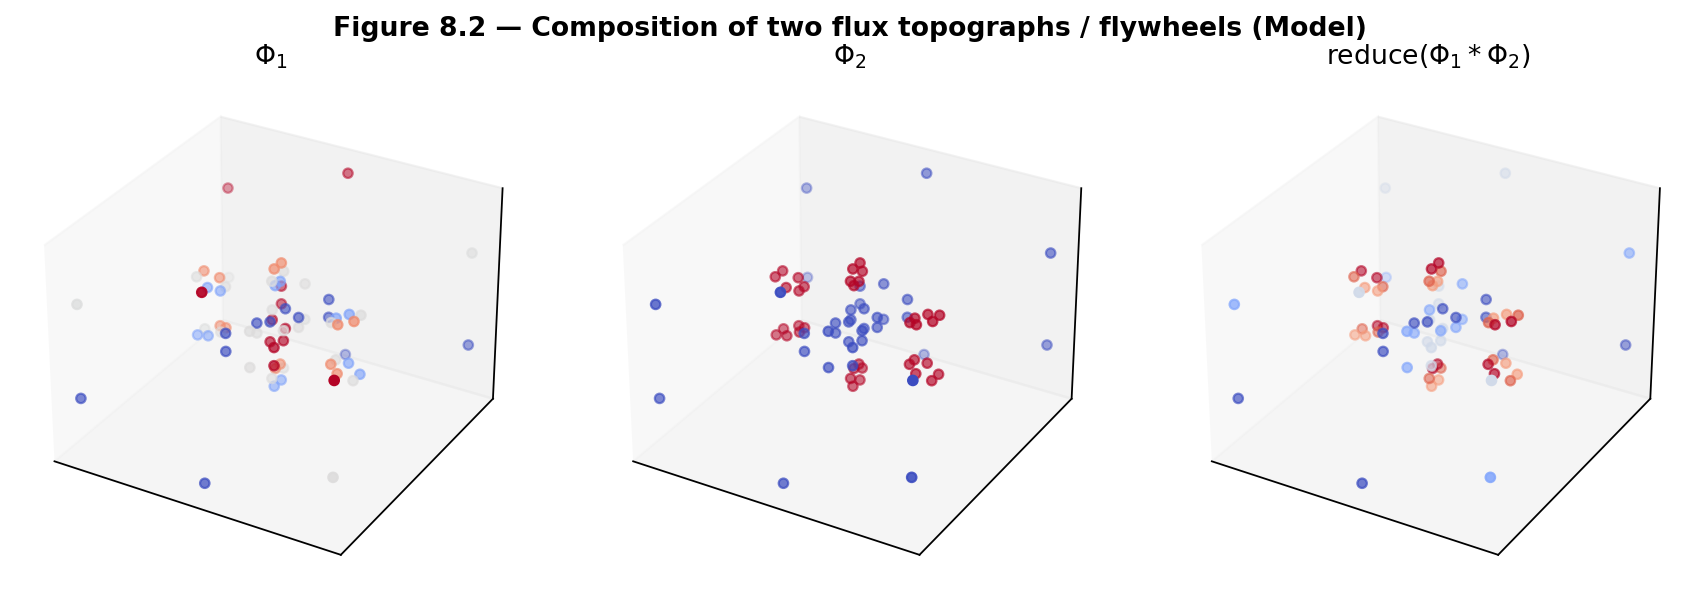
\includegraphics[width=0.92\textwidth,height=0.42\textheight,keepaspectratio]{fig8_2_flywheel_composition.png}
  \caption{Figure 8.2 --- Composition of two flux topographs.}
  \label{fig:fig8-2-flywheel-composition}
\end{figure}

\begin{quote}\small\textit{Figure 8.2.* \(\Phi_1\), \(\Phi_2\), and \(\mathrm{reduce}(\Phi_1*\Phi_2)\) for the pedagogical \texttt{value\_sum} method.}\end{quote}

\textbf{Honest status.} On current candidate adjacency and modest angle lattices, composition tables often show \textbf{poor closure} and \textbf{low associativity scores} (\textbf{Software fact} from the sandbox). That is not a failure of the chapter---it is the experimental content of \textbf{Open Problem 6}.

\textbf{Open Problem 6 (core of this chapter).} Does a well-defined, associative composition law exist on equivalence classes of flux configurations / flywheels that:

\begin{enumerate}
\item Reduces to classical Gauss composition under a suitable projection or restriction?  
\item Is compatible with the gauge actions of Chapter 4?  
\item Produces a finite (or finitely generated) abelian group whose order/structure predicts Magic Island counts?
\end{enumerate}

Sandbox: \texttt{qga/lib/composition.py}. Depends on OP1--OP3.

\bigskip
\noindent\rule{\textwidth}{0.4pt}
\bigskip

\section{8.3 Class-group analogues}
\label{ch:ch08_class_group:8-3-class-group-analogues}

The set of equivalence classes of reduced flux topographs, equipped with a composition law, forms a \textbf{class-group analogue}. Its order is a \textbf{class-number analogue}---related to Chapter 6's \texttt{class\_number\_analogue}, now enriched by composition tables and associativity diagnostics.

\begin{lstlisting}[style=qga]
class_group_analogue(topo_or_list, method=..., dedup_tol=...)
  -> order, structure, table, closure_fraction, associativity, representatives

composition_table(reduced_set)
is_associative_up_to_equivalence(reduced_set, samples=...)
\end{lstlisting}

\begin{figure}[htbp]
  \centering
  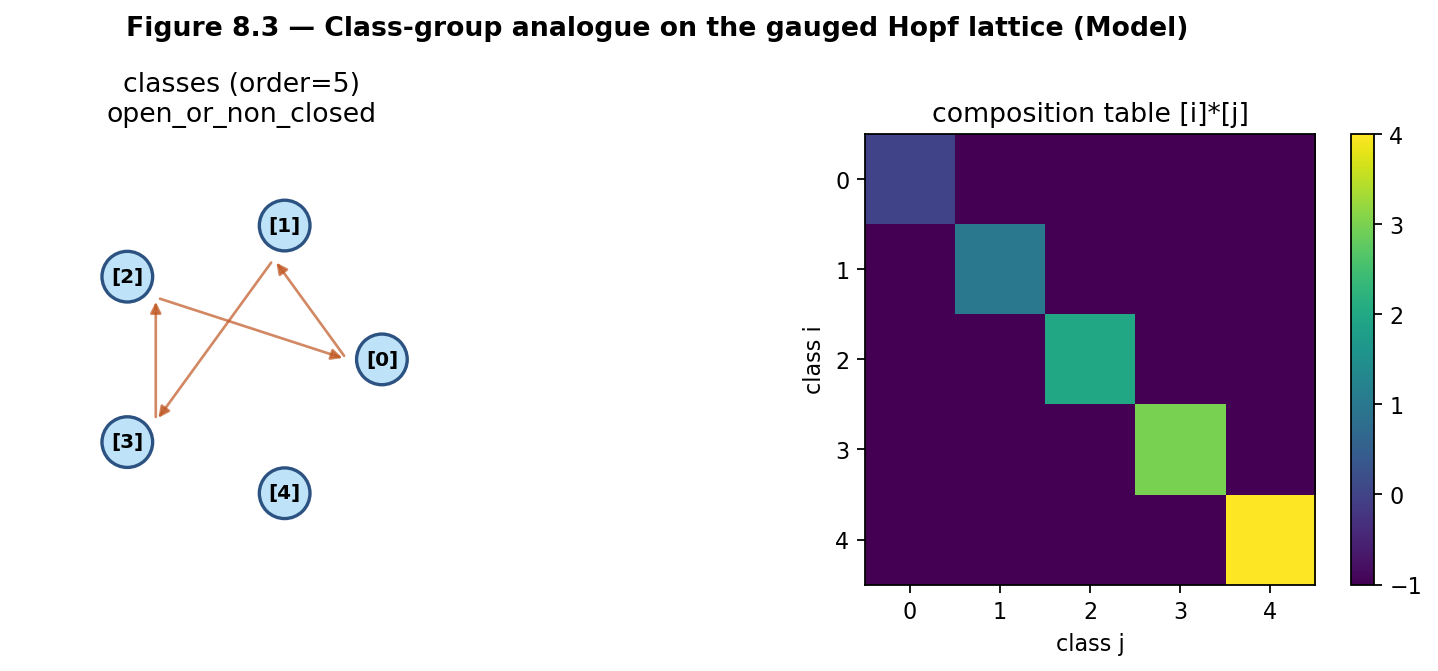
\includegraphics[width=0.92\textwidth,height=0.42\textheight,keepaspectratio]{fig8_3_class_group_analogue.png}
  \caption{Figure 8.3 --- Class-group analogue.}
  \label{fig:fig8-3-class-group-analogue}
\end{figure}

\begin{quote}\small\textit{Figure 8.3.* Equivalence classes with composition arrows, plus a numerical composition table. \texttt{structure} strings such as \texttt{partial\_magma} or \texttt{open\_or\_non\_closed} flag OP6 incompleteness.}\end{quote}

Magic Islands can be viewed as \textbf{distinguished classes} (or clusters of classes) where composition yields high \texttt{magic\_island\_score} or high portal \texttt{stability\_score}. Predicting islands from group structure alone is OP3 ? OP6.

\begin{figure}[htbp]
  \centering
  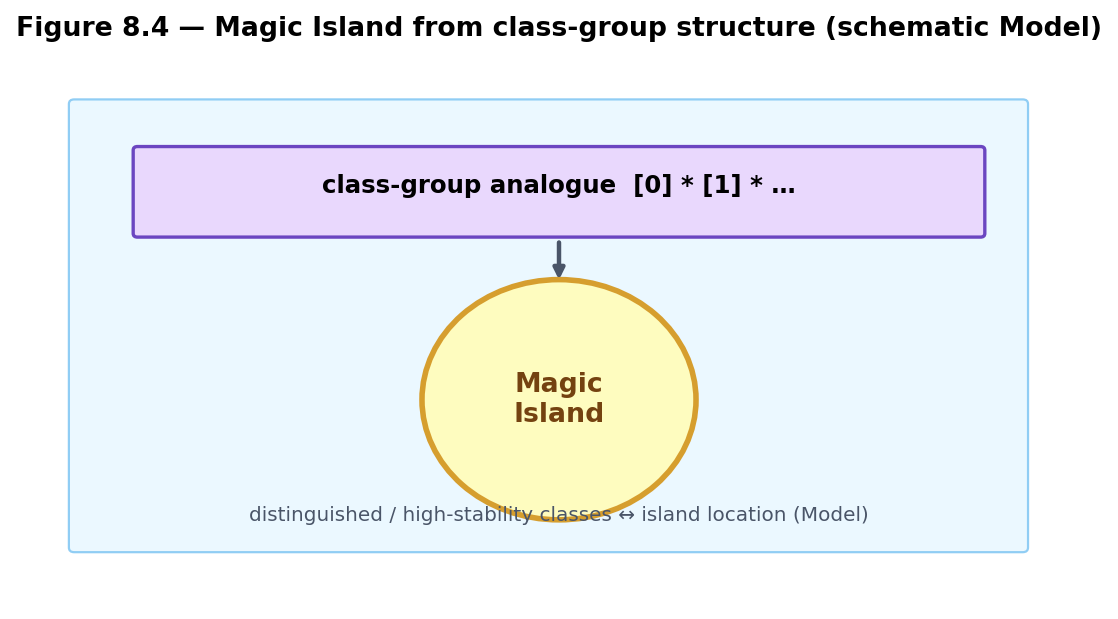
\includegraphics[width=0.92\textwidth,height=0.42\textheight,keepaspectratio]{fig8_4_island_from_class.png}
  \caption{Figure 8.4 --- Magic Island from class-group data.}
  \label{fig:fig8-4-island-from-class}
\end{figure}

\begin{quote}\small\textit{Figure 8.4.* Schematic: class-group analogue \(\rightarrow\) distinguished high-stability region. \textbf{Model} narrative, not a derived theorem.}\end{quote}

\begin{figure}[htbp]
  \centering
  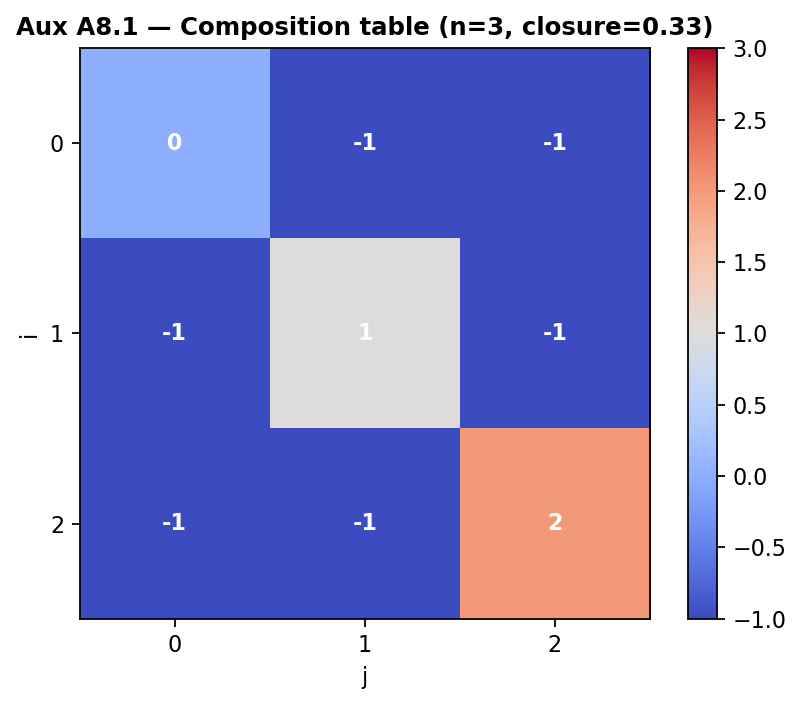
\includegraphics[width=0.92\textwidth,height=0.42\textheight,keepaspectratio]{aux8_1_composition_table.png}
  \caption{Auxiliary Figure A8.1 --- Composition table.}
  \label{fig:aux8-1-composition-table}
\end{figure}

\begin{quote}\small\textit{Auxiliary Figure A8.1.* Small \(n\times n\) table of reduced class indices under composition. Entries \(-1\) mean ``not closed in the set within tolerance.''}\end{quote}

\bigskip
\noindent\rule{\textwidth}{0.4pt}
\bigskip

\section{8.4 First computational labs}
\label{ch:ch08_class_group:8-4-first-computational-labs}

Helpers: \texttt{lib/composition.py} \(\cdot\) \textbf{Appendix C ?C.4}.

\begin{itemize}
\item \textbf{8.A} \texttt{compose\_flywheels} + \texttt{reduce\_composition}.
\item \textbf{8.B} \texttt{composition\_table} / \texttt{closure\_fraction}.
\item \textbf{8.C} \texttt{class\_group\_analogue} order and structure.
\item \textbf{8.D} \texttt{is\_associative\_up\_to\_equivalence} (expect low scores --- OP6 data).
\item \textbf{8.E} Optional: compare composition methods.
\end{itemize}

\begin{lstlisting}[style=qga,language=python]
from lib.composition import compose_flywheels, reduce_composition
# build t1, t2 as in Appendix C ?C.4
# print(reduce_composition(compose_flywheels(t1, t2))["classification"]["type"])
\end{lstlisting}

\bigskip
\noindent\rule{\textwidth}{0.4pt}
\bigskip

\section{Exercises}
\label{ch:ch08_class_group:exercises}

\textbf{8.A (hand).} State Gauss composition for binary quadratic forms in one sentence and explain why it produces a group law on classes.

\textbf{8.B (hand).} Why is associativity (up to equivalence) the key property needed for a class-group analogue?

\textbf{8.C (code).} Complete Labs 8.A--8.B. Report the type of the composed configuration and the composition table's \texttt{closure\_fraction}.

\textbf{8.D (code).} Complete Lab 8.C. What is the size of the class-group analogue on your seed topograph?

\textbf{8.E (code).} Run Lab 8.D. What associativity score do you obtain? Record failures.

\textbf{8.F (Hatcher bridge).} In Hatcher, the class group encodes the failure of unique factorization in quadratic fields. Sketch how a class-group analogue on the Hopf lattice might encode ``failure of unique representation'' by stable flywheels / \(Z\)-map preimages.

\textbf{8.G (Open Problem 6 teaser).} Using \texttt{compose\_flywheels} and \texttt{is\_associative\_up\_to\_equivalence}, test associativity on the current candidate adjacency. Document numerical failures---they \emph{are} OP6 progress.

\textbf{8.H (forward).} Why will the quaternion algebra theory of Chapter 9 be the natural home for a rigorous version of these class groups?

\textbf{8.I (software honesty).} Distinguish: (i) classical class groups (\textbf{Theorem}), (ii) \texttt{class\_group\_analogue} outputs (\textbf{Model} + software), (iii) any claim that Magic Islands \emph{are} class groups of a quaternion order (\textbf{Hypothesis} until proved).

\bigskip
\noindent\rule{\textwidth}{0.4pt}
\bigskip

\section{Code and asset pointers}
\label{ch:ch08_class_group:code-and-asset-pointers}

\begin{lstlisting}[style=qga]
qga/lib/composition.py
qga/lib/flux_topograph.py
qga/lib/hopf_lattice.py
kingdom.core.flux_flywheel   # optional cross-check with Z stability
\end{lstlisting}

\textbf{Figures:} \texttt{scripts/generate\_ch8\_figures.py} \textbf{Open problems:} OP6 (this chapter); depends on OP1--OP3. \textbf{Related portal:} no dedicated composition tab yet---Lattice Simulator / Flux Flywheel remain dynamical counterparts.

\bigskip
\noindent\rule{\textwidth}{0.4pt}
\bigskip

\section{Looking ahead}
\label{ch:ch08_class_group:looking-ahead}

We now have a working \textbf{Model} lift of Gauss composition and the class group to flux configurations on the gauged Hopf lattice---with explicit experimental gaps (closure, associativity). In \textbf{Chapter 9} we move to quaternion algebras and their ideal theory, the rigorous arithmetic home for class groups of orders (Hurwitz, Eichler, ...). \textbf{Chapter 10} returns to observational validation, including whether class-group structure predicts \(350/\pi\) or \(Z\)-map patterns.

With composition and class-group language in place, we are ready for the ideal-theoretic foundation.

\bigskip
\noindent\rule{\textwidth}{0.4pt}
\bigskip



% Auto-generated from book/09_quaternion_algebras.md — do not edit by hand
% Regenerated by scripts/md_to_latex.py

\chapter{Chapter 9 --- Quaternion Algebras and Ideal Theory}
\label{ch:ch09_algebras}

This chapter supplies the rigorous algebraic foundation for the class-group analogues and composition laws of Chapter 8. We introduce quaternion algebras over \(\mathbb{Q}\), their orders (especially the Hurwitz order), and the ideal theory that turns equivalence classes of ideals into a group. This framework is the natural home for making the Model constructions of previous chapters more arithmetic and for attacking Open Problem 6 with algebraic tools.

\textbf{Learning goals}

\begin{enumerate}
\item Define quaternion algebras over \(\mathbb{Q}\) and understand ramification.  
\item Work with orders (Lipschitz, Hurwitz, maximal) and their ideal theory.  
\item See how ideal classes form a group and how this relates to the class-group analogues of Chapter 8.  
\item Connect ideal theory back to composition of forms / flywheels and to Magic Islands (\textbf{Model} dictionary).  
\item Prepare algebraic language for rigorous uniqueness and composition statements (OP6 and beyond).  
\item Separate \textbf{algebraic}, \textbf{sequential-label}, and \textbf{angle-lock} invariants when discrete moduli label continuous geometric orbits (supporting stack \texttt{vortex\_\allowbreak{}math}).
\end{enumerate}

\textbf{Figures in this chapter}

\begin{center}
\small
\setlength{\tabcolsep}{4pt}
\begin{tabularx}{\textwidth}{@{}>{\raggedright\arraybackslash}p{0.12\textwidth}>{\raggedright\arraybackslash}X>{\raggedright\arraybackslash}X@{}}
\toprule
Tag & File & Role \\
\midrule
Fig. 9.1 & \texttt{figures/\allowbreak{}fig9\_\allowbreak{}1\_\allowbreak{}quaternion\_\allowbreak{}algebra.\allowbreak{}png} & Quaternion algebra ramification diagram \\
Fig. 9.2 & \texttt{figures/\allowbreak{}fig9\_\allowbreak{}2\_\allowbreak{}hurwitz\_\allowbreak{}order.\allowbreak{}png} & Hurwitz order units / comparison \\
Fig. 9.3 & \texttt{figures/\allowbreak{}fig9\_\allowbreak{}3\_\allowbreak{}ideal\_\allowbreak{}class\_\allowbreak{}group.\allowbreak{}png} & Ideal class group schematic \\
Fig. 9.4 & \texttt{figures/\allowbreak{}fig9\_\allowbreak{}4\_\allowbreak{}ideal\_\allowbreak{}to\_\allowbreak{}flywheel.\allowbreak{}png} & Ideal class \(\rightarrow\) flywheel (Model bridge) \\
Fig. 9.5 & \texttt{figures/\allowbreak{}fig9\_\allowbreak{}5\_\allowbreak{}modulus\_\allowbreak{}invariants.\allowbreak{}png} & Three-layer modulus invariants (algebra \(\cdot\) flow \(\cdot\) lock control) \\
Aux A9.1 & \texttt{figures/\allowbreak{}aux9\_\allowbreak{}1\_\allowbreak{}ramification\_\allowbreak{}table.\allowbreak{}png} & Hilbert-symbol ramification table \\
\bottomrule
\end{tabularx}
\end{center}


\textbf{Claim discipline}

\begin{center}
\small
\setlength{\tabcolsep}{4pt}
\begin{tabularx}{\textwidth}{@{}>{\raggedright\arraybackslash}X>{\raggedright\arraybackslash}X@{}}
\toprule
Claim & Type \\
\midrule
Quaternion algebras, Hilbert symbols, Hurwitz Euclidean property, Hurwitz class number 1 & \textbf{Theorem} (classical) \\
Dictionary between ideal classes and flux topographs / Magic Islands & \textbf{Model} \\
Separation of modulus invariants on irrational rotations (algebra vs progression vs angle lock) & \textbf{Model} (experimentally controlled; not a theorem of TN) \\
\texttt{qga/\allowbreak{}lib/\allowbreak{}quaternion\_\allowbreak{}algebra.\allowbreak{}py} helpers; external \texttt{vortex\_\allowbreak{}math} metrics & \textbf{Software fact} \\
\bottomrule
\end{tabularx}
\end{center}


\bigskip
\noindent\rule{\textwidth}{0.4pt}
\bigskip

\section{9.1 Quaternion algebras over \(\mathbb{Q}\)}
\label{ch:ch09_algebras:9-1-quaternion-algebras-over-mathbb-q}

A \textbf{quaternion algebra} over \(\mathbb{Q}\) is a 4-dimensional central simple algebra over \(\mathbb{Q}\). Up to isomorphism, each is given by square-free integers \(a,b\neq 0\) via

\[
\Bigl(\frac{a,b}{\mathbb{Q}}\Bigr)
=
\mathbb{Q}+\mathbb{Q}i+\mathbb{Q}j+\mathbb{Q}ij,
\qquad
i^2=a,\; j^2=b,\; ij=-ji.
\]

The Hamilton algebra corresponds (over \(\mathbb{R}\)) to \(a=b=-1\); as an algebra over \(\mathbb{Q}\) one studies \(\bigl(\frac{-1,-1}{\mathbb{Q}}\bigr)\).

\subsection{Ramification}
\label{ch:ch09_algebras:ramification}

At each place \(p\) (finite prime or \(\infty\)), the local Hilbert symbol \((a,b)_p\in\{\pm 1\}\) detects whether the algebra is a division algebra (\(-1\), \textbf{ramified}) or isomorphic to \(M_2\) (\textbf{split}). The set of ramified places is finite and of even cardinality; it classifies the algebra.

\begin{lstlisting}[style=qga]
QuaternionAlgebra(a, b)
  .ramified_places()
  .is_definite()          # True iff ramified at ?
  .hilbert_at(p)
\end{lstlisting}

\begin{figure}[htbp]
  \centering
  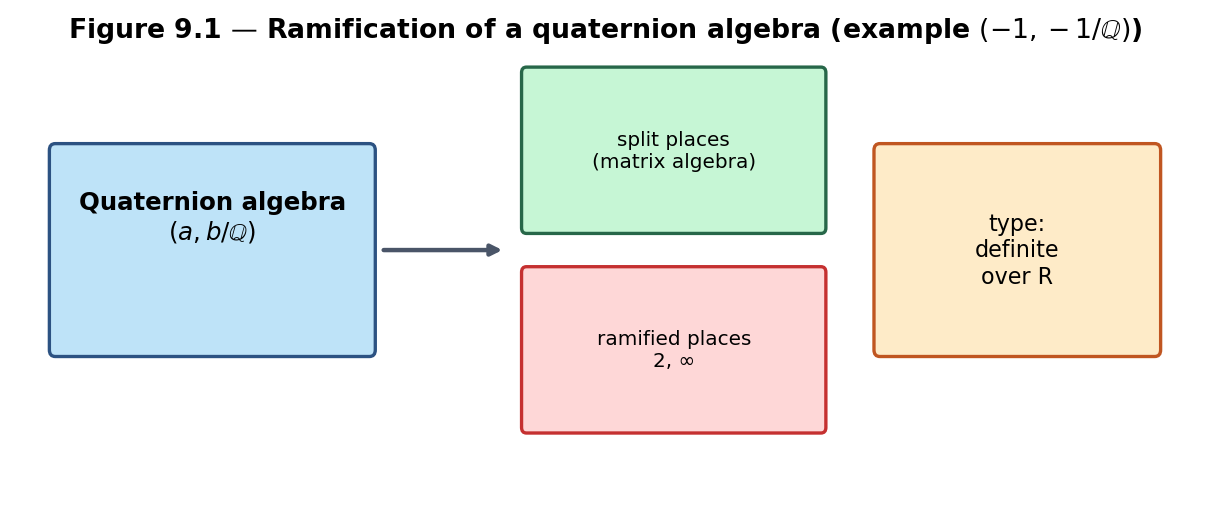
\includegraphics[width=0.92\textwidth,height=0.42\textheight,keepaspectratio]{fig9_1_quaternion_algebra.png}
  \caption{Figure 9.1 --- Ramification of a quaternion algebra.}
  \label{fig:fig9-1-quaternion-algebra}
\end{figure}

\begin{quote}\small\textit{Figure 9.1.* Example \(\bigl(\frac{-1,-1}{\mathbb{Q}}\bigr)\): ramified at \(2\) and \(\infty\) (definite over \(\mathbb{R}\)).}\end{quote}

\begin{figure}[htbp]
  \centering
  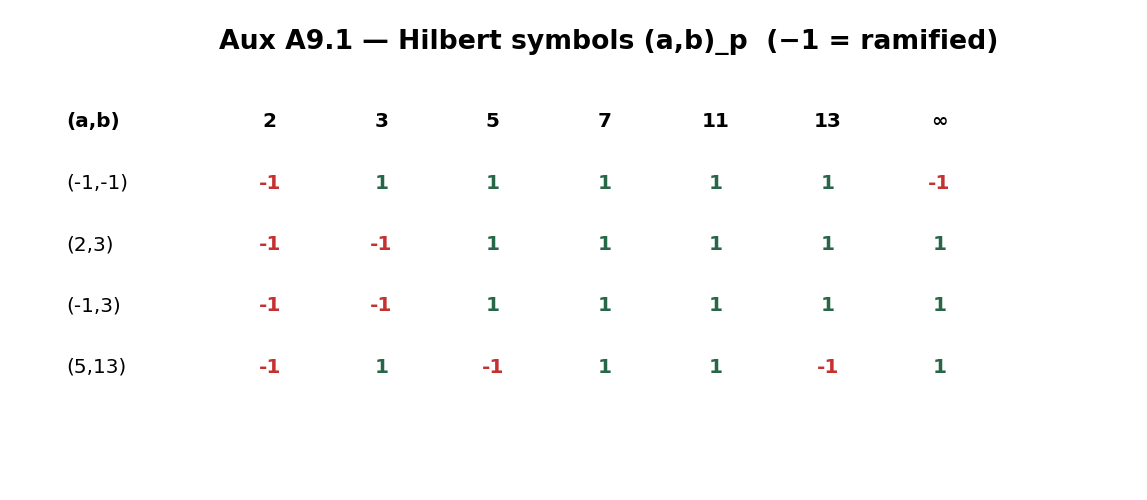
\includegraphics[width=0.92\textwidth,height=0.42\textheight,keepaspectratio]{aux9_1_ramification_table.png}
  \caption{Auxiliary Figure A9.1 --- Hilbert-symbol table.}
  \label{fig:aux9-1-ramification-table}
\end{figure}

\begin{quote}\small\textit{Auxiliary Figure A9.1.* Hilbert symbols for several \((a,b)\) at small places; red \(-1\) marks ramification.}\end{quote}

\textbf{Claim type.} Classification by ramification sets and Hilbert symbols: \textbf{Theorem} (classical). Implementation in the book helper: \textbf{Software fact} (pedagogical, not a full number-theory library).

\bigskip
\noindent\rule{\textwidth}{0.4pt}
\bigskip

\section{9.2 Orders in quaternion algebras}
\label{ch:ch09_algebras:9-2-orders-in-quaternion-algebras}

An \textbf{order} is a subring that is a full-rank \(\mathbb{Z}\)-lattice in the algebra. In the Hamilton setting:

\begin{center}
\small
\setlength{\tabcolsep}{4pt}
\begin{tabularx}{\textwidth}{@{}>{\raggedright\arraybackslash}X>{\raggedright\arraybackslash}X>{\raggedright\arraybackslash}X>{\raggedright\arraybackslash}X@{}}
\toprule
Order & Definition & Units & Euclidean? \\
\midrule
Lipschitz & \(\mathbb{Z}[i,j,k]\) & 8 & No \\
Hurwitz & all-integer or all-half-integer coords & 24 & Yes (maximal) \\
\bottomrule
\end{tabularx}
\end{center}


The Hurwitz order is preferred for arithmetic (Chapter 1 \textbf{Model} preference for lattice work; Euclidean algorithm is classical \textbf{Theorem}). Its unit group is the binary tetrahedral group---the set \(\Lambda_0\) of Chapter 3.

\begin{figure}[htbp]
  \centering
  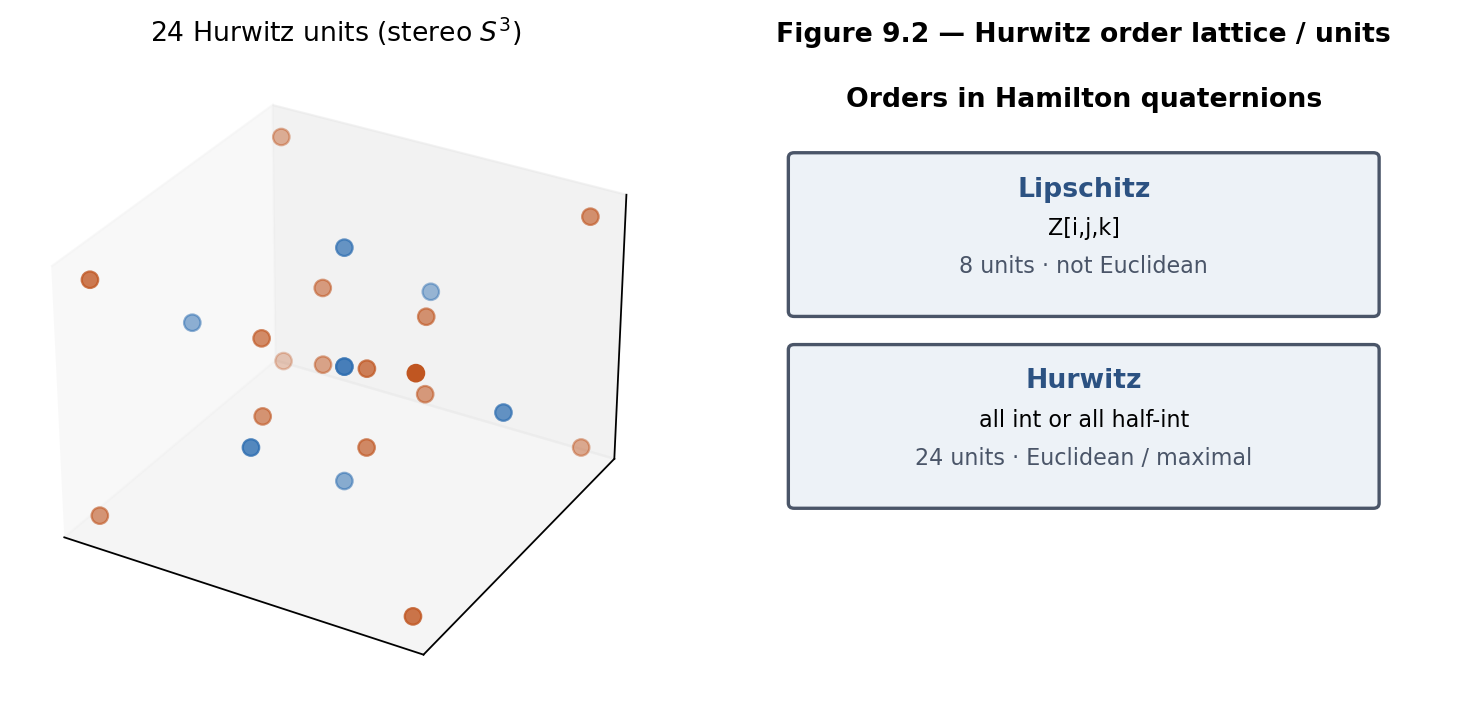
\includegraphics[width=0.92\textwidth,height=0.42\textheight,keepaspectratio]{fig9_2_hurwitz_order.png}
  \caption{Figure 9.2 --- Hurwitz order.}
  \label{fig:fig9-2-hurwitz-order}
\end{figure}

\begin{quote}\small\textit{Figure 9.2.* 24 Hurwitz units in stereographic \(S^3\), and Lipschitz vs Hurwitz comparison.}\end{quote}

\begin{lstlisting}[style=qga]
HurwitzOrder().units          # 24
HurwitzOrder().is_euclidean() # True (classical fact)
HurwitzOrder().is_maximal()   # True (classical fact)
LipschitzOrder().n_units()    # 8
\end{lstlisting}

In general quaternion algebras, \textbf{maximal orders} play the role of rings of integers in number fields; different maximal orders need not be conjugate when the class number is nontrivial.

\bigskip
\noindent\rule{\textwidth}{0.4pt}
\bigskip

\section{9.3 Ideal theory and class groups}
\label{ch:ch09_algebras:9-3-ideal-theory-and-class-groups}

One studies left ideals, right ideals, and two-sided ideals of an order. For \textbf{definite} quaternion algebras (ramified at \(\infty\)), the left ideal class set of a maximal order is finite. Ideal multiplication induces a group structure on (two-sided) ideal classes, and related class sets control representation of integers by norms of ideals.

\subsection{Hurwitz class number (classical)}
\label{ch:ch09_algebras:hurwitz-class-number-classical}

The left ideal class number of the Hurwitz order is \textbf{1}: every left ideal is principal. The book helper reports this as a cited classical fact with a finite sample check of small-norm elements---not a full ideal enumeration.

\begin{lstlisting}[style=qga]
left_ideal_class_group(HurwitzOrder())
  -> IdealClassGroupResult(order=1, method='classical_hurwitz_class_number_one', ...)
\end{lstlisting}

\begin{figure}[htbp]
  \centering
  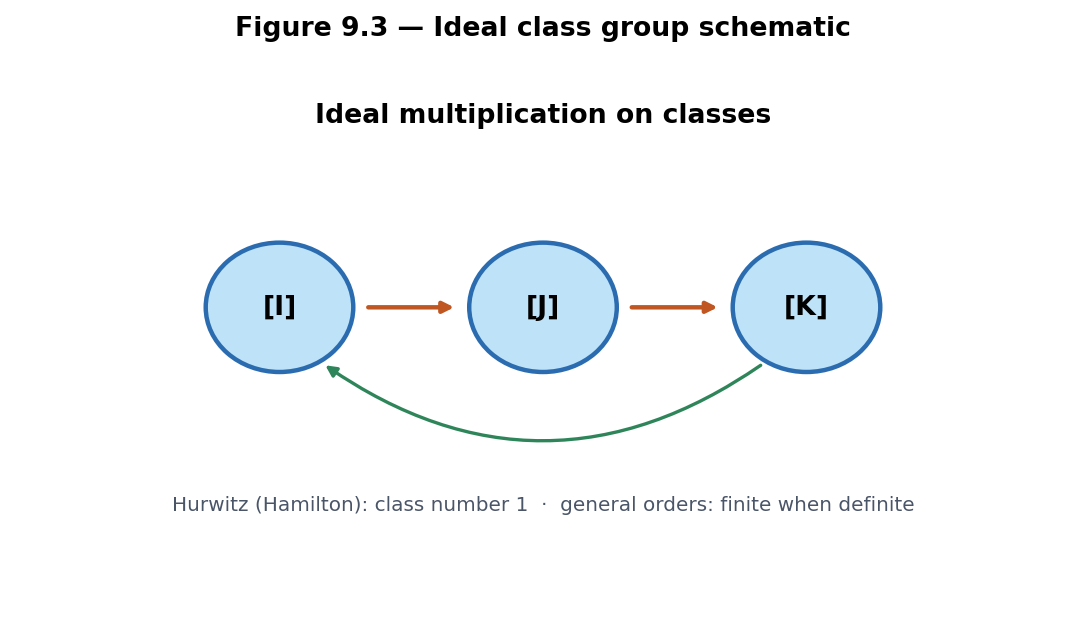
\includegraphics[width=0.92\textwidth,height=0.42\textheight,keepaspectratio]{fig9_3_ideal_class_group.png}
  \caption{Figure 9.3 --- Ideal class group schematic.}
  \label{fig:fig9-3-ideal-class-group}
\end{figure}

\begin{quote}\small\textit{Figure 9.3.* Ideal classes with multiplication. For Hurwitz, a single class; general definite orders may have larger finite class numbers.}\end{quote}

\textbf{Claim type.} Finiteness for definite maximal orders; Hurwitz class number 1: \textbf{Theorem} (classical). Full algorithmic enumeration of ideals for general \((a,b)\): out of scope for this sandbox.

\bigskip
\noindent\rule{\textwidth}{0.4pt}
\bigskip

\section{9.4 From ideals to flux topographs and flywheels (Model bridge)}
\label{ch:ch09_algebras:9-4-from-ideals-to-flux-topographs-and-flywheels-model-bridg}

Chapter 8 approximated class groups with composition of flux topographs. The natural dictionary is still a \textbf{Model}:

\begin{center}
\small
\setlength{\tabcolsep}{4pt}
\begin{tabularx}{\textwidth}{@{}>{\raggedright\arraybackslash}X>{\raggedright\arraybackslash}X@{}}
\toprule
Algebraic object & Geometric / Model object \\
\midrule
Ideal in a quaternion order & Flux configuration / supporting cycle on the gauged Hopf lattice \\
Ideal class & Equivalence class of reduced flux topographs \\
Ideal class group & Class-group analogue of Chapter 8 \\
Norm of an ideal & Stability score or \texttt{magic\_\allowbreak{}island\_\allowbreak{}score} \\
Ideal multiplication & Composition of flywheels (when well-defined --- OP6) \\
\bottomrule
\end{tabularx}
\end{center}


\begin{figure}[htbp]
  \centering
  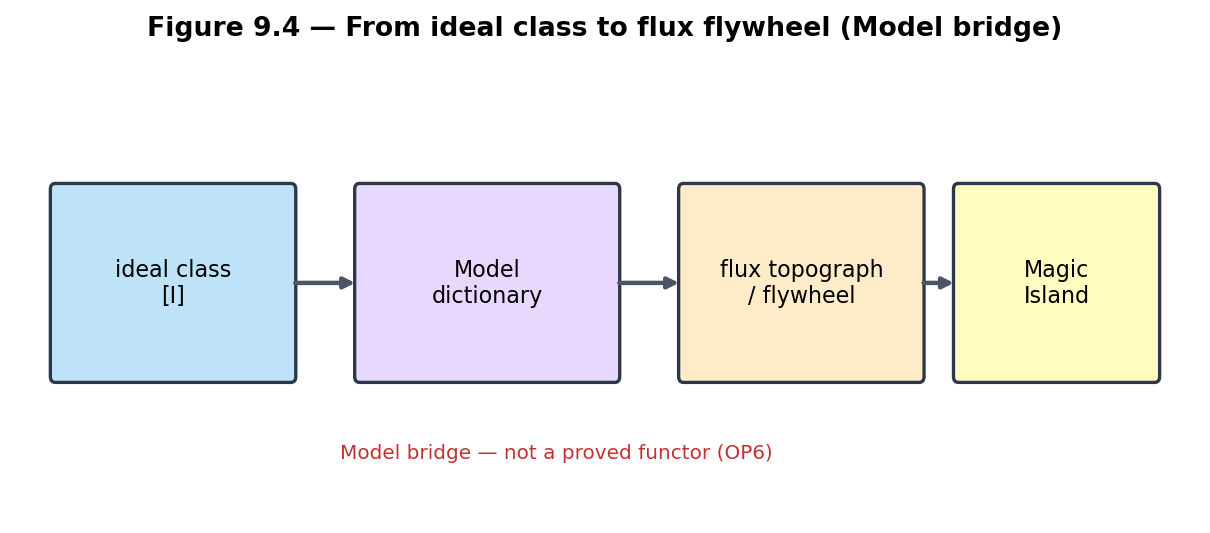
\includegraphics[width=0.92\textwidth,height=0.42\textheight,keepaspectratio]{fig9_4_ideal_to_flywheel.png}
  \caption{Figure 9.4 --- From ideal class to flux flywheel.}
  \label{fig:fig9-4-ideal-to-flywheel}
\end{figure}

\begin{quote}\small\textit{Figure 9.4.* Schematic Model bridge. Not a proved functor.}\end{quote}

\textbf{Open Problem 6 (continued).} Use ideal theory of quaternion algebras to define a rigorous composition law on classes of flux configurations that is associative, gauge-compatible, and reduces to Gauss composition in suitable limits. Determine whether the resulting class group predicts Magic Island location and size.

\begin{lstlisting}[style=qga]
form_ideal_dictionary_entry()   # static dictionary for labs
class_group_analogue(...)       # Ch. 8 Model side
left_ideal_class_group(...)     # algebraic side (Hurwitz: order 1)
\end{lstlisting}

\bigskip
\noindent\rule{\textwidth}{0.4pt}
\bigskip

\section{9.5 Modulus, invariants, and angle--label locking}
\label{ch:ch09_algebras:9-5-modulus-invariants-and-angle-label-locking}

*Supporting stack: \href{https://github.com/kinaar8340/vortex_math}{\texttt{vortex\_\allowbreak{}math}} \(\cdot\) research note: \href{../notes/RESEARCH_NOTE_moduli.md}{\texttt{notes/\allowbreak{}RESEARCH\_\allowbreak{}NOTE\_\allowbreak{}moduli.\allowbreak{}md}}.*

Chapters 3--8 build discrete geometric objects (gauged Hopf lattice, flux topographs) whose \textbf{labels} and \textbf{equivalence classes} carry arithmetic meaning. Before those dictionaries become too ambitious, it is worth isolating a cleaner, lower-dimensional lesson: when symbolic patterns of Vortex Math---digital roots, the doubling circuit, and the privileged status of 3-6-9---are placed onto points generated by \emph{continuous geometry} rather than discrete integer sequences alone, the choice of labeling modulus does \textbf{not} act as a single uniform operator. It modifies \emph{different invariants} depending on how it is attached to the system.

\subsection{Geometric stage}
\label{ch:ch09_algebras:geometric-stage}

Consider an irrational rotation on the unit circle whose step size is a fixed multiple of the circle constant:

\[
\theta_k = k \cdot \frac{9}{\pi} \pmod{2\pi}.
\]

Because \(9/\pi\) is an irrational multiple of \(2\pi\), the orbit is dense: successive points come arbitrarily close to every location on the circle without closing into a finite regular polygon. The factor \textbf{9} echoes the digital-root base of Vortex Math; \textbf{?} is the circle's own constant. Geometry and numerology share the stage, but they are no longer forced to play the same role. (A coupled step \(\Delta\theta = m/\pi\) will appear below when the modulus is allowed to set the winding rate.)

\subsection{Three layers of invariant}
\label{ch:ch09_algebras:three-layers-of-invariant}

\textbf{Algebraic structure of the doubling map.} Changing the modulus alters the cycle decomposition of repeated doubling on \(\mathbb{Z}/m\mathbb{Z}\). The value \(m = 37\) produces the cleanest long orbit: length 36 from 1, with 2 acting as a primitive root modulo 37. Composites built from 37---notably \(111 = 3 \times 37\) and \(333 = 9 \times 37\)---inherit this long cycle length but fragment it according to the Chinese Remainder Theorem. Algebraic ``cleanness'' is therefore strongest at the repunit prime \textbf{37}, the prime factor of the length-3 repunit \(R_3 = 111\).

\textbf{Orderly progression of labels along the geometric orbit.} When the rotational step itself is \emph{coupled} to the modulus (\(\Delta\theta = m/\pi\)), labels advance with greater sequential coherence for certain composites. The value \textbf{111} frequently yields the highest scores for label progression and overall symmetry under this coupled regime. Here the modulus influences the \emph{flow of labels relative to the accumulating points}, rather than the intrinsic algebraic cycles alone. Composite structure and winding rate interact; the prime-mover number 111 is not merely decorative in this layer.

\textbf{Positional angle--label locking.} Only one labeling method creates a genuine \emph{statistical} dependence between label and actual geometric angle: explicit angular binning (\texttt{angle\_\allowbreak{}bin}). Under the default sequential method (\texttt{step\_\allowbreak{}index})---labels from the step count and its digital root or modular residue---normalized mutual information between labels and angles remains at or below chance once a proper null model (label shuffling with the same marginals) is applied.

Apparent visual symmetry in sequential plots therefore reflects \textbf{orderly sequential progression}, not a hidden locking of labels to preferred angles on the circle. That outcome is precisely what one should expect from an irrational rotation labeled by step index: the orbit has no preferred angles unless the labeling method itself introduces angular bins by construction.

\begin{figure}[htbp]
  \centering
  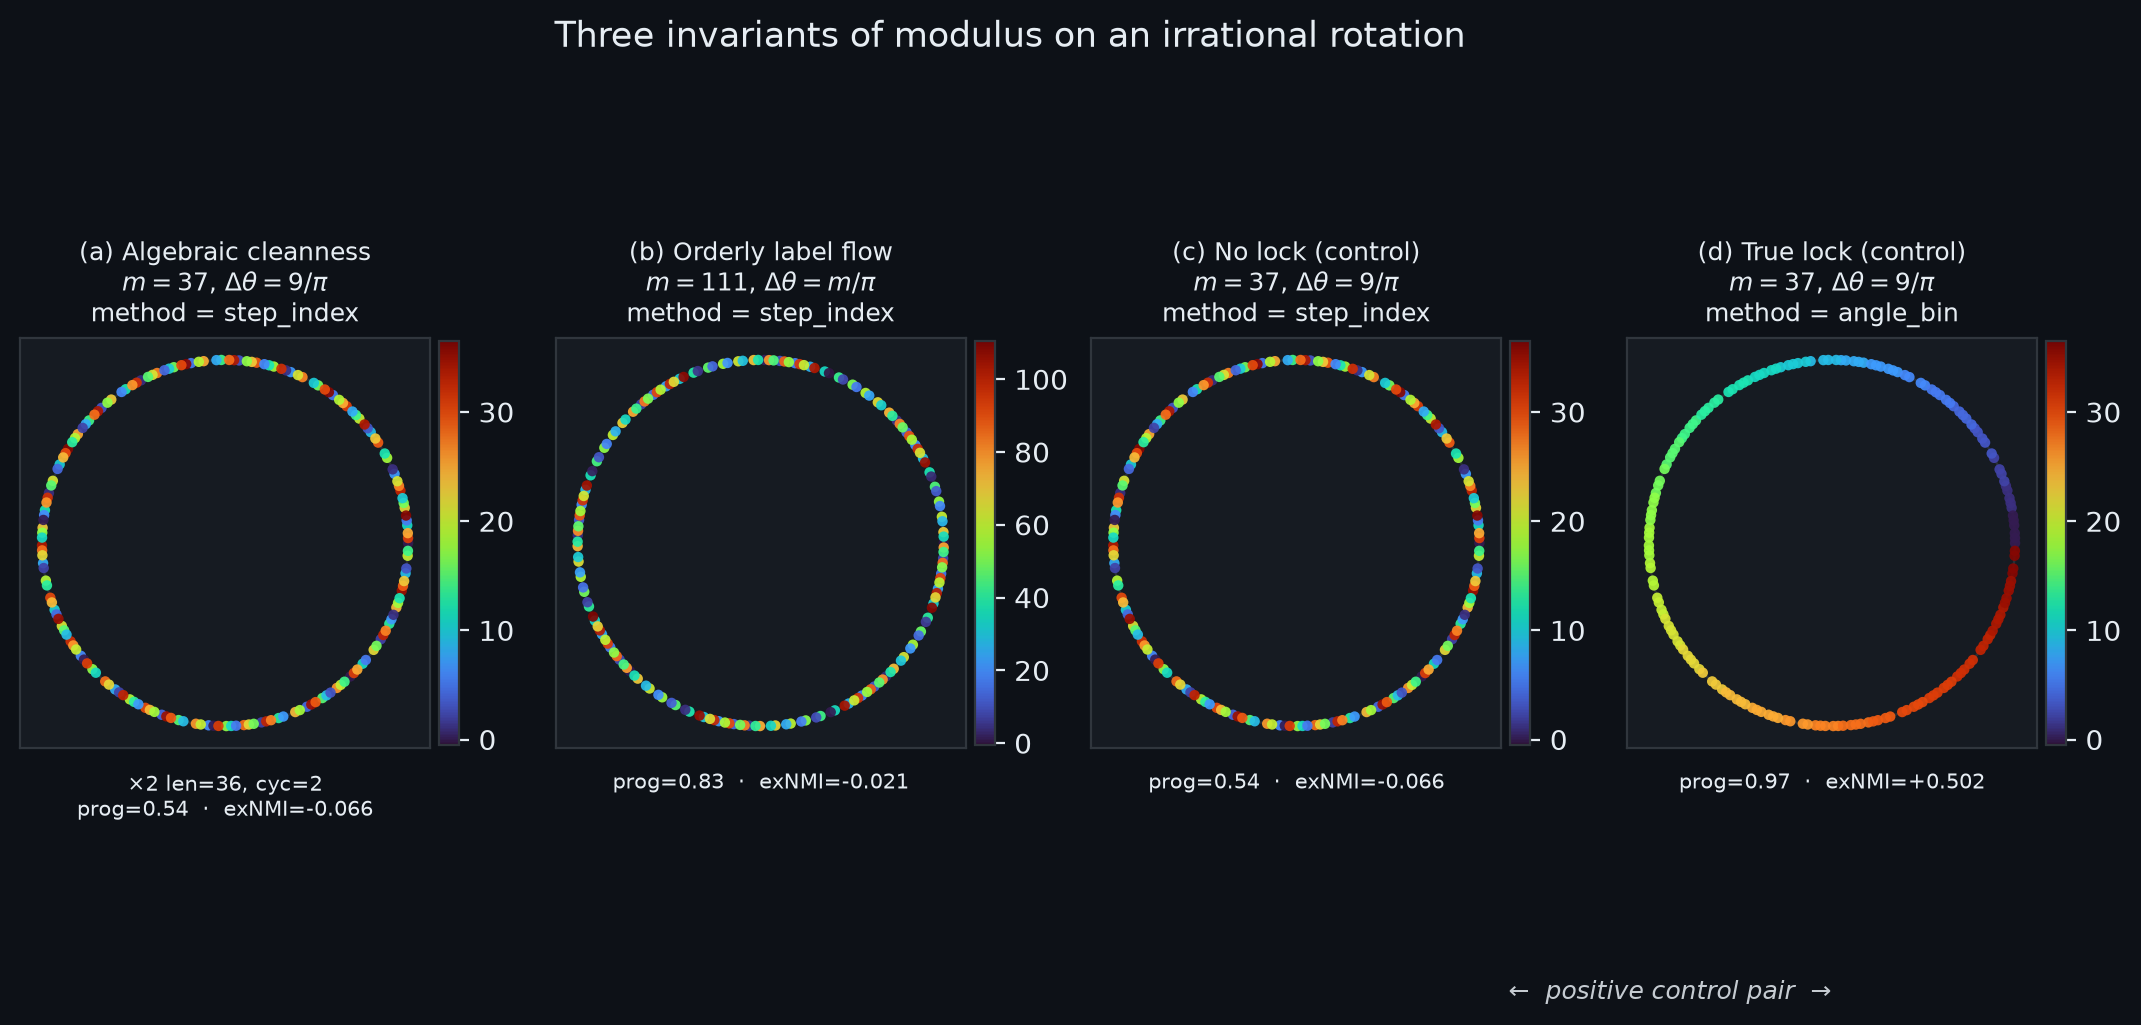
\includegraphics[width=0.92\textwidth,height=0.42\textheight,keepaspectratio]{fig9_5_modulus_invariants.png}
  \caption{Figure 9.5 --- Three invariants of modulus on an irrational rotation.}
  \label{fig:fig9-5-modulus-invariants}
\end{figure}

\begin{quote}\small\textit{Figure 9.5.* \textbf{(a)} Algebraic cleanness: \(m=37\), fixed step \(9/\pi\), sequential labels---long clean \(\times 2\) structure. \textbf{(b)} Orderly label flow: \(m=111\), coupled step \(m/\pi\), sequential labels---higher label-progression along the orbit. \textbf{(c)--(d)} Positive control pair at \(m=37\): sequential labeling yields excess NMI at or below the shuffle null; angular binning yields strongly positive excess NMI. Visual order under step-index is progression, not positional lock. *(Supporting generation: \texttt{vortex\_\allowbreak{}math} \(\cdot\) \texttt{assets/\allowbreak{}book\_\allowbreak{}figure\_\allowbreak{}three\_\allowbreak{}layers.\allowbreak{}png}.)}\end{quote}

\subsection{Controls and claim type}
\label{ch:ch09_algebras:controls-and-claim-type}

These layers were separated by controlled comparisons of mapping methods, step modes, and quantitative metrics: excess normalized mutual information (\textbf{exNMI}) against permutation baselines, label-progression scores, and angular uniformity. A positive control seals the analysis: when labels \emph{are} angle bins, exNMI is strongly positive and many standard deviations above the null; when labels are step indices, exNMI is not.

\textbf{Claim type.} The three-layer separation and control are a \textbf{Model} for how arithmetic moduli interact with geometric orbits in this book's ecosystem---experimentally reproducible, not a classical theorem of Hatcher \emph{Topology of Numbers}. Implementation and full tables: \textbf{Software fact} (\texttt{vortex\_\allowbreak{}math} repo; note in \texttt{notes/\allowbreak{}RESEARCH\_\allowbreak{}NOTE\_\allowbreak{}moduli.\allowbreak{}md}).

\subsection{Takeaway for the QGA spine}
\label{ch:ch09_algebras:takeaway-for-the-qga-spine}

The practical consequence is concise:

> \textbf{Modulus changes the algebraic and sequential-label invariants; it does not create angle--label locking on an irrational rotation unless you label by angle itself.}

This distinguishes synchronicity that arises from composite number structure---notably \textbf{111} as prime-mover composite \(3 \times 37\)---from stronger geometric claims that would require explicit angular construction. Algebra crowns 37; coupled progression frequently crowns 111 under the \(m/\pi\) regime; true positional locking belongs only to labeling methods that bin explicitly by angle.

For the rest of the book: when Chapters 5--8 speak of ``labels,'' ``classes,'' and ``Magic Islands,'' the same discipline applies---\textbf{name which invariant you are measuring}. Ideal class groups (?9.3--9.4) are algebraic invariants; flux scores and topograph diagrams are geometric or Model-level; statistical lock to a continuous base space is a third claim, and must be tested against a null, not inferred from visual order alone.

\begin{lstlisting}[style=qga]
# External supporting stack (not vendored in lib/)
~/Projects/vortex_math
  python src/main.py --family-37 --num-steps 200
  python src/main.py --resonance-scan --method step_index --num-steps 600
  python src/main.py --resonance-scan --method angle_bin --num-steps 600
\end{lstlisting}

\bigskip
\noindent\rule{\textwidth}{0.4pt}
\bigskip

\section{9.6 First computational labs}
\label{ch:ch09_algebras:9-6-first-computational-labs}

Helpers: \texttt{lib/\allowbreak{}quaternion\_\allowbreak{}algebra.\allowbreak{}py} \(\cdot\) \textbf{Appendix C ?C.4}.

\begin{itemize}
\item \textbf{9.A} \texttt{QuaternionAlgebra(-1,-1).\allowbreak{}ramified\_\allowbreak{}places()}.
\item \textbf{9.B} Hurwitz: 24 units, Euclidean, maximal.
\item \textbf{9.C} \texttt{left\_\allowbreak{}ideal\_\allowbreak{}class\_\allowbreak{}group} \(\rightarrow\) class number 1 (cited classical).
\item \textbf{9.D} Compare algebraic order 1 vs Model \texttt{class\_\allowbreak{}group\_\allowbreak{}analogue} order.
\item \textbf{9.E} Hilbert symbols table.
\item \textbf{9.F (optional, external)} Run the \texttt{vortex\_\allowbreak{}math} resonance control: \texttt{step\_\allowbreak{}index} vs \texttt{angle\_\allowbreak{}bin} and record exNMI signs.
\end{itemize}

\begin{lstlisting}[style=qga,language=python]
from lib.quaternion_algebra import QuaternionAlgebra, HurwitzOrder, left_ideal_class_group
print(QuaternionAlgebra(-1, -1).ramified_places())
print(HurwitzOrder().n_units(), left_ideal_class_group().order)
\end{lstlisting}

\bigskip
\noindent\rule{\textwidth}{0.4pt}
\bigskip

\section{Exercises}
\label{ch:ch09_algebras:exercises}

\textbf{9.A (hand).} Define a quaternion algebra over \(\mathbb{Q}\) and state what ramification means.

\textbf{9.B (hand).} Why is the Hurwitz order preferred over the Lipschitz order for most arithmetic work?

\textbf{9.C (code).} Complete Labs 9.A--9.B. Confirm 24 Hurwitz units and Euclidean / maximal flags.

\textbf{9.D (code).} Run Lab 9.C. What class number do you obtain for Hurwitz, and what does the \texttt{method} string say?

\textbf{9.E (code).} Complete Lab 9.D. Compare algebraic class number \(1\) with the Model \texttt{class\_\allowbreak{}group\_\allowbreak{}analogue} order. Why can they differ?

\textbf{9.F (Hatcher bridge).} In Hatcher Chapter 8, forms correspond to ideals. Sketch how ?9.4's dictionary might be made precise for a quaternion order (even if only conjecturally).

\textbf{9.G (Open Problem 6).} Using Hurwitz class number 1, what would a \emph{successful} OP6 composition law look like when restricted to configurations ``coming from'' principal ideals? What obstructions remain for non-principal classes in other algebras?

\textbf{9.H (forward).} Why will Chapter 10's observational validation benefit from a rigorous ideal-theoretic home for class-group analogues?

\textbf{9.I (software honesty).} Distinguish: (i) classical ideal class groups (\textbf{Theorem}), (ii) \texttt{left\_\allowbreak{}ideal\_\allowbreak{}class\_\allowbreak{}group} toy report (\textbf{software} citing theorem), (iii) Ch. 8 \texttt{class\_\allowbreak{}group\_\allowbreak{}analogue} (\textbf{Model}).

\textbf{9.J (modulus invariants).} In section 9.5, name the three layers (algebra / progression / angle lock). Which modulus wins algebraic cleanness? Which often wins progression under \(m/\pi\)? Why is positive exNMI under \texttt{angle\_\allowbreak{}bin} a \emph{control}, not a discovery about \(m=37\)?

\textbf{9.K (code, external).} If \texttt{\textasciitilde{}\allowbreak{}/\allowbreak{}Projects/\allowbreak{}vortex\_\allowbreak{}math} is available, run Lab 9.F and report exNMI under \texttt{step\_\allowbreak{}index} vs \texttt{angle\_\allowbreak{}bin} for \(m\in\{9,37,111\}\).

\bigskip
\noindent\rule{\textwidth}{0.4pt}
\bigskip

\section{Code and asset pointers}
\label{ch:ch09_algebras:code-and-asset-pointers}

\begin{lstlisting}[style=qga]
qga/lib/quaternion_algebra.py
  QuaternionAlgebra, hilbert_symbol,
  HurwitzOrder, LipschitzOrder,
  left_ideal_class_group, form_ideal_dictionary_entry

qga/lib/composition.py
qga/lib/hopf_lattice.py   # HURWITZ_UNITS shared with Ch. 3

# Supporting stack (external)
~/Projects/vortex_math/          # active development
qga/lib/vortex_math/README.md    # pointer into this book's tree
qga/notes/RESEARCH_NOTE_moduli.md
\end{lstlisting}

\textbf{Figures:} \texttt{scripts/\allowbreak{}generate\_\allowbreak{}ch9\_\allowbreak{}figures.\allowbreak{}py} \(\cdot\) Fig. 9.5 from \texttt{vortex\_\allowbreak{}math} book figure \textbf{Open problems:} OP6 (composition via ideal theory); OP1--OP3 for the geometric side of the dictionary. \textbf{Research note:} \texttt{notes/\allowbreak{}RESEARCH\_\allowbreak{}NOTE\_\allowbreak{}moduli.\allowbreak{}md}

\bigskip
\noindent\rule{\textwidth}{0.4pt}
\bigskip

\section{Looking ahead}
\label{ch:ch09_algebras:looking-ahead}

We now have the algebraic backbone---quaternion algebras, orders, and ideal class groups---that can host rigorous versions of the Model constructions in Chapters 5--8, together with a controlled lesson on \textbf{which invariant a modulus is measuring} when discrete labels meet continuous orbits. In \textbf{Chapter 10} we return to the observational layer: statistical protocols for \(350/\pi\), the \(Z\mapsto\) map, Magic Islands, and any class-group predictions that become precise enough to test---always distinguishing algebraic claims, Model dictionaries, and empirical lock statistics.

With the ideal-theoretic foundation in place, the full construction is ready for observational scrutiny.

\bigskip
\noindent\rule{\textwidth}{0.4pt}
\bigskip




\part{Observations and Models}
% Auto-generated from book/10_observations_emergent.md — do not edit by hand
% Regenerated by scripts/md_to_latex.py

\chapter{Chapter 10 --- Observations, Hypotheses, and Validation}
\label{ch:ch10_observations}

This chapter collects the observational layer of the Kingdom Come Model. It presents the recurring numerical signature \(W_g = 350/\pi\), the \(Z\mapsto\) flux map correlations, Magic Island alignments, and other multi-domain patterns. All claims here are labeled explicitly as \textbf{Model} or \textbf{Hypothesis}, and the chapter supplies concrete validation protocols (Table \textbf{T4}) so that the construction can be tested, refined, or falsified.

\textbf{Learning goals}

\begin{enumerate}
\item Review the major observational signatures that motivated the project.  
\item Distinguish Model statements from testable Hypotheses.  
\item Apply the validation protocols to the \(350/\pi\) signature and the \(Z\mapsto\) map.  
\item Summarize the status of all Open Problems.  
\item Provide a clear roadmap for future empirical work.
\end{enumerate}

\textbf{Figures in this chapter}

\begin{center}
\small
\setlength{\tabcolsep}{4pt}
\begin{tabularx}{\textwidth}{@{}>{\raggedright\arraybackslash}p{0.12\textwidth}>{\raggedright\arraybackslash}X>{\raggedright\arraybackslash}X@{}}
\toprule
Tag & File & Role \\
\midrule
Fig. 10.1 & \texttt{figures/\allowbreak{}fig10\_\allowbreak{}1\_\allowbreak{}350\_\allowbreak{}over\_\allowbreak{}pi\_\allowbreak{}domains.\allowbreak{}png} & Multi-domain recurrence of \(350/\pi\) \\
Fig. 10.2 & \texttt{figures/\allowbreak{}fig10\_\allowbreak{}2\_\allowbreak{}z\_\allowbreak{}map\_\allowbreak{}correlation.\allowbreak{}png} & Stability score vs chemical proxy \\
Fig. 10.3 & \texttt{figures/\allowbreak{}fig10\_\allowbreak{}3\_\allowbreak{}magic\_\allowbreak{}island\_\allowbreak{}validation.\allowbreak{}png} & Islands vs observed specialness \\
Fig. 10.4 & \texttt{figures/\allowbreak{}fig10\_\allowbreak{}4\_\allowbreak{}validation\_\allowbreak{}flowchart.\allowbreak{}png} & Validation protocol (Table T4) \\
Aux A10.1 & \texttt{figures/\allowbreak{}aux10\_\allowbreak{}1\_\allowbreak{}pulsar\_\allowbreak{}bitcoin\_\allowbreak{}overlay.\allowbreak{}png} & Pulsar / Bitcoin observation assets \\
\bottomrule
\end{tabularx}
\end{center}


\textbf{Claim discipline (throughout the book)}

\begin{center}
\small
\setlength{\tabcolsep}{4pt}
\begin{tabularx}{\textwidth}{@{}>{\raggedright\arraybackslash}X>{\raggedright\arraybackslash}X@{}}
\toprule
Label & Meaning \\
\midrule
\textbf{Theorem} & Proved here or classical \\
\textbf{Model} & Consistent mathematical or physical construction, not claimed as nature's unique law \\
\textbf{Hypothesis} & Observational claim needing validation or falsification \\
\textbf{Software fact} & Reproducible output of a named implementation \\
\bottomrule
\end{tabularx}
\end{center}


\textbf{Invariant discipline (from Chapter 9 section 9.5).} When reading or testing observations, also name \emph{which invariant} is at stake:

\begin{center}
\small
\setlength{\tabcolsep}{4pt}
\begin{tabularx}{\textwidth}{@{}>{\raggedright\arraybackslash}p{0.12\textwidth}>{\raggedright\arraybackslash}X>{\raggedright\arraybackslash}X@{}}
\toprule
Layer & Question & Example in this chapter \\
\midrule
Algebraic & Does a discrete arithmetic object have a clean structure? & Ideal class number; composition law (OP6) \\
Sequential / Model flow & Do labels or scores progress coherently along a construction? & Stability scores along \(Z\); topograph evolution \\
Statistical lock & Is there dependence on a continuous base beyond chance? & Multi-domain recurrence of \(350/\pi\) vs null (Table T4) \\
\bottomrule
\end{tabularx}
\end{center}


Visual order and multi-domain co-occurrence are \emph{not} automatic geometric lock. Chapter 9's modulus lesson (and its \texttt{angle\_\allowbreak{}bin} control) is the template: measure excess association against a null, do not infer locking from appearance alone. Research note: \texttt{notes/\allowbreak{}RESEARCH\_\allowbreak{}NOTE\_\allowbreak{}moduli.\allowbreak{}md}.

\bigskip
\noindent\rule{\textwidth}{0.4pt}
\bigskip

\section{10.1 The major observational signatures}
\label{ch:ch10_observations:10-1-the-major-observational-signatures}

The Kingdom Come project was motivated by several recurring numerical and structural patterns:

\begin{itemize}
\item The constant
\end{itemize}

\[
  W_g = \frac{350}{\pi} \approx 111.408
\]

(\texttt{WG\_\allowbreak{}FROM\_\allowbreak{}350\_\allowbreak{}OVER\_\allowbreak{}PI} in Kingdom Come / book helper \texttt{WG\_\allowbreak{}350\_\allowbreak{}OVER\_\allowbreak{}PI}) appearing across pulsar-timing narratives, Bitcoin Pi Cycle notes, TLS tree analysis, cuprate sketches, and structural constants.

\begin{itemize}
\item Alignment of high \texttt{stability\_\allowbreak{}score} regions (Magic Islands) with noble-gas \(Z\) and selected mid-table elements.  
\item Topological protection (linked Hopf fibers) as a geometric language for stability that classical elementary number theory only hints at.
\end{itemize}

These patterns live in the portal \textbf{Observations} tab and in \texttt{kingdom/\allowbreak{}observations/\allowbreak{}}.

\begin{figure}[htbp]
  \centering
  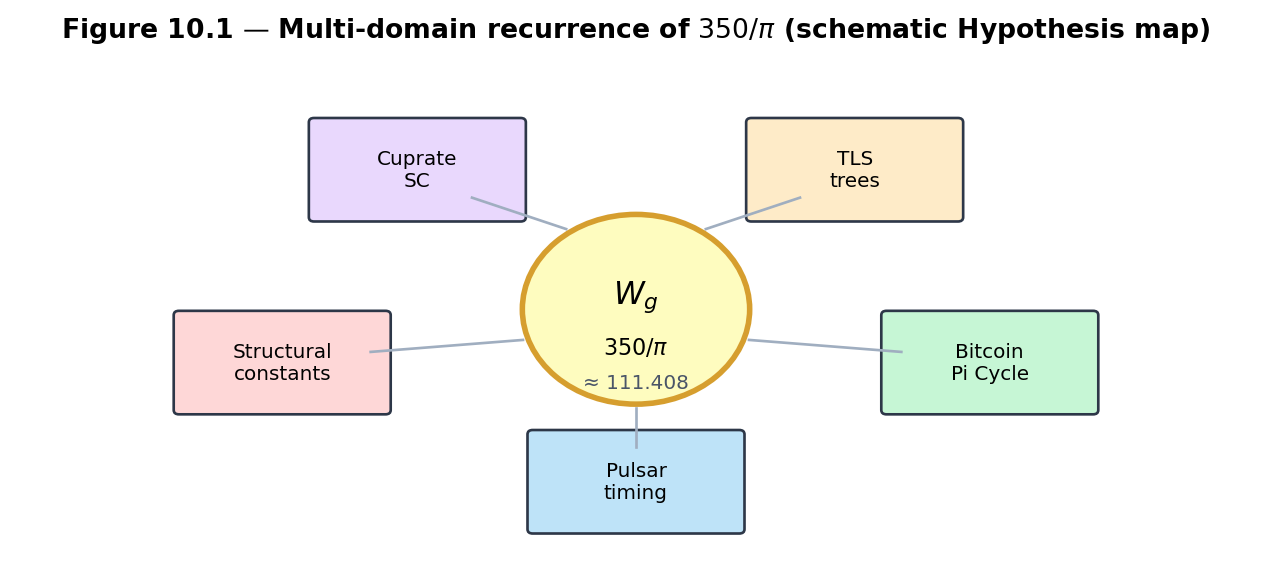
\includegraphics[width=0.92\textwidth,height=0.42\textheight,keepaspectratio]{fig10_1_350_over_pi_domains.png}
  \caption{Figure 10.1 --- Multi-domain recurrence of \(350/\pi\).}
  \label{fig:fig10-1-350-over-pi-domains}
\end{figure}

\begin{quote}\small\textit{Figure 10.1.* Domains associated with the \(W_g=350/\pi\) signature in the observation program (schematic).}\end{quote}

\textbf{Claim type.} Raw portal constants and plotted observation assets: \textbf{software / project facts}. The claim that they share a single topological clock: \textbf{Hypothesis} (OP5).

\begin{figure}[htbp]
  \centering
  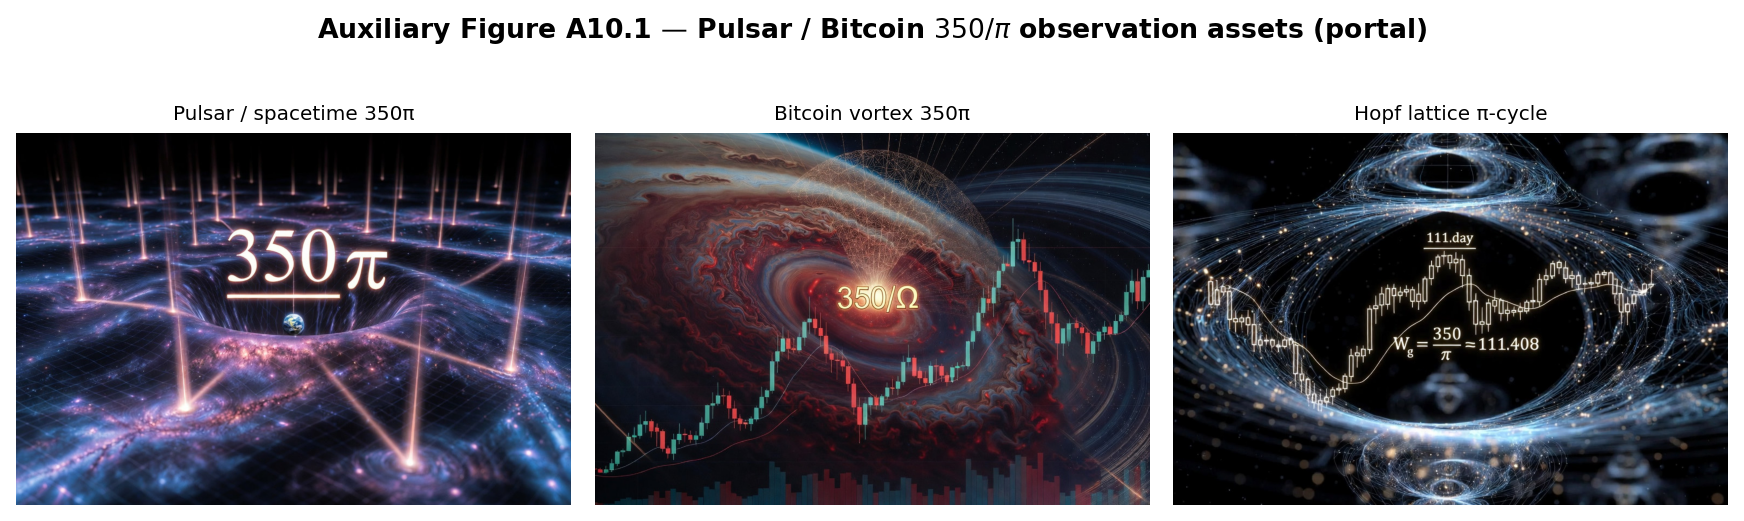
\includegraphics[width=0.92\textwidth,height=0.42\textheight,keepaspectratio]{aux10_1_pulsar_bitcoin_overlay.png}
  \caption{Auxiliary Figure A10.1 --- Pulsar / Bitcoin assets.}
  \label{fig:aux10-1-pulsar-bitcoin-overlay}
\end{figure}

\begin{quote}\small\textit{Auxiliary Figure A10.1.* Portal observation assets (pulsar spacetime \(350\pi\), Bitcoin vortex / lattice ?-cycle). Visual motivation only---not a completed statistical test.}\end{quote}

\bigskip
\noindent\rule{\textwidth}{0.4pt}
\bigskip

\section{10.2 The \(Z\mapsto\) flux map --- current status}
\label{ch:ch10_observations:10-2-the-z-mapsto-flux-map-current-status}

Chapter 7 defined

\[
Z \mapsto \bigl(\text{flywheel state},\;\texttt{stability\_score},\;\texttt{stability\_class},\;\ldots\bigr)
\]

via \texttt{map\_\allowbreak{}z\_\allowbreak{}to\_\allowbreak{}flywheel} / \texttt{map\_\allowbreak{}z\_\allowbreak{}to\_\allowbreak{}flywheel\_\allowbreak{}extended}. Outputs show peaks near noble-gas \(Z\) and partial alignment with ionization-energy proxies in extended fields.

\begin{figure}[htbp]
  \centering
  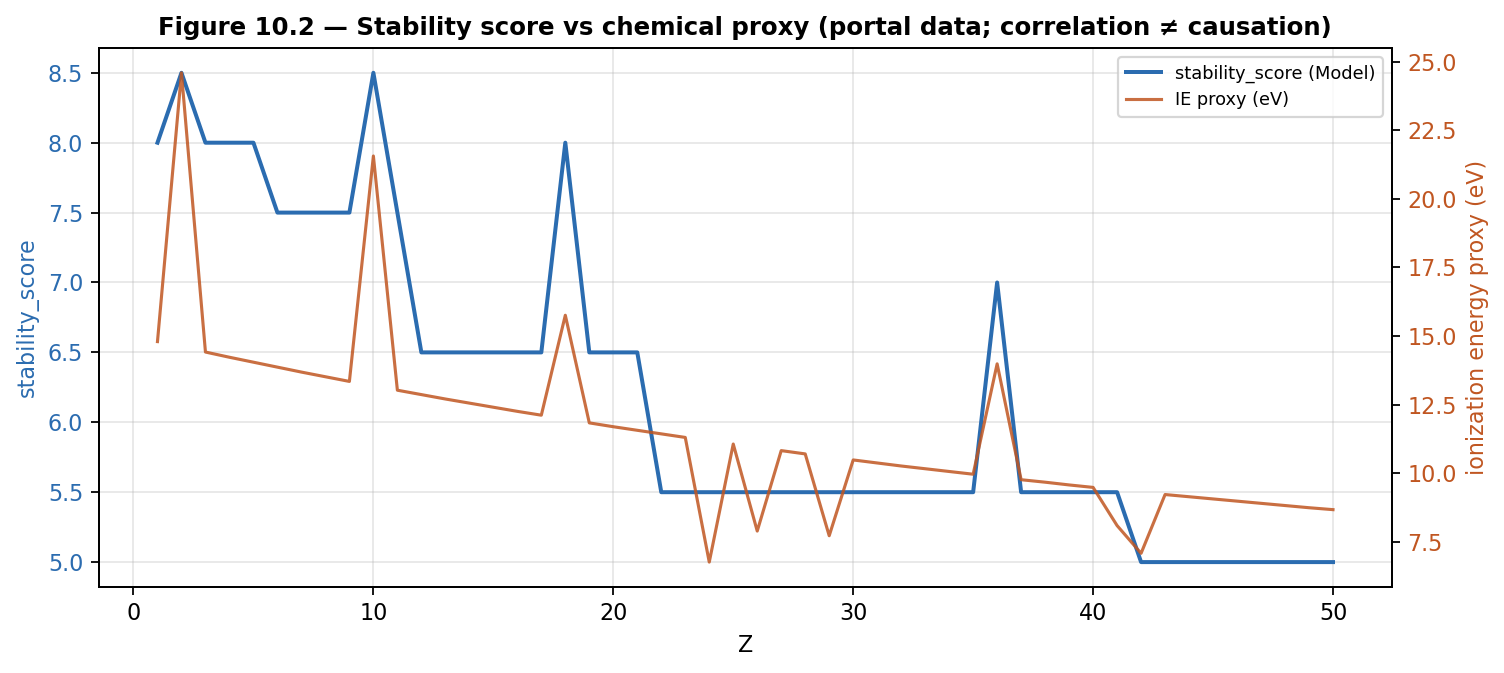
\includegraphics[width=0.92\textwidth,height=0.42\textheight,keepaspectratio]{fig10_2_z_map_correlation.png}
  \caption{Figure 10.2 --- Stability score vs chemical proxy.}
  \label{fig:fig10-2-z-map-correlation}
\end{figure}

\begin{quote}\small\textit{Figure 10.2.* Portal \texttt{stability\_\allowbreak{}score} vs an IE proxy across \(Z\). \textbf{Correlation is not causation}; ablation and out-of-sample tests are required (Table T4).}\end{quote}

\textbf{Claim type.} Reproducible curves from the current implementation: \textbf{Software fact}. Physical emergence of the periodic table: \textbf{Model} / \textbf{Hypothesis}.

\textbf{Open Problem 4 (recap).} Up to gauge, is the \(Z\mapsto\) flywheel map unique under stated axioms? See Chapter 7 and \texttt{notes/\allowbreak{}open\_\allowbreak{}problems.\allowbreak{}md}.

\bigskip
\noindent\rule{\textwidth}{0.4pt}
\bigskip

\section{10.3 Magic Islands and chemical/nuclear specialness}
\label{ch:ch10_observations:10-3-magic-islands-and-chemical-nuclear-specialness}

Magic Islands (Chapters 5--6) appear as regions of high periodicity, controlled variance, and high \texttt{stability\_\allowbreak{}score} / \texttt{magic\_\allowbreak{}island\_\allowbreak{}score}. Some coincide with elements that are chemically or nuclearly special.

\begin{figure}[htbp]
  \centering
  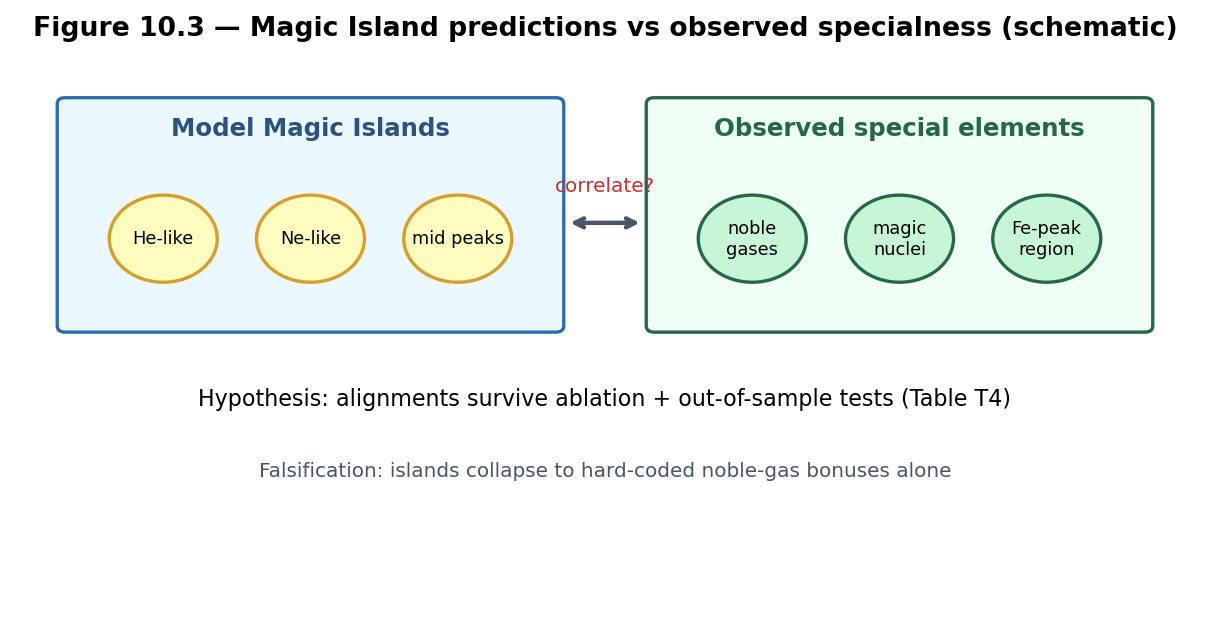
\includegraphics[width=0.92\textwidth,height=0.42\textheight,keepaspectratio]{fig10_3_magic_island_validation.png}
  \caption{Figure 10.3 --- Magic Island predictions vs observed specialness.}
  \label{fig:fig10-3-magic-island-validation}
\end{figure}

\begin{quote}\small\textit{Figure 10.3.* Model islands vs observed special classes (schematic). Encouraging correlation inside the working Model---not yet derived from first principles.}\end{quote}

\textbf{Falsification sketch.} If ablating explicit noble-gas bonuses removes all predictive alignment with held-out properties, the ``emergence'' reading of islands fails the Table T4 protocol for that claim.

\bigskip
\noindent\rule{\textwidth}{0.4pt}
\bigskip

\section{10.4 Summary of Open Problems}
\label{ch:ch10_observations:10-4-summary-of-open-problems}

\begin{center}
\small
\setlength{\tabcolsep}{4pt}
\begin{tabularx}{\textwidth}{@{}>{\raggedright\arraybackslash}X>{\raggedright\arraybackslash}X>{\raggedright\arraybackslash}X>{\raggedright\arraybackslash}X@{}}
\toprule
\# & Problem & Home & Status (one line) \\
\midrule
OP1 & Canonical quaternionic Farey & Ch. 3 & Open --- \texttt{candidate\_\allowbreak{}adjacency} \\
OP2 & Flux topograph axioms & Ch. 5 & Open --- \texttt{flux\_\allowbreak{}topograph} \\
OP3 & Class number \(\leftrightarrow\) Magic Island & Ch. 6 & Open --- heuristic \\
OP4 & \(Z\to\) flywheel uniqueness & Ch. 7 / 10 & Open \\
OP5 & \(350/\pi\) first principles / falsify & Ch. 10 & Open --- Table T4 \\
OP6 & Flywheel composition (Gauss lift) & Ch. 8--9 & Open --- low sandbox closure \\
\bottomrule
\end{tabularx}
\end{center}


\textbf{Full statements, sandboxes, success criteria, and dependency sketch:} \textbf{Appendix B}. Helpers: \texttt{lib.\allowbreak{}validation.\allowbreak{}open\_\allowbreak{}problems\_\allowbreak{}status\_\allowbreak{}table()}.

\bigskip
\noindent\rule{\textwidth}{0.4pt}
\bigskip

\section{10.5 Validation protocols (Table T4)}
\label{ch:ch10_observations:10-5-validation-protocols-table-t4}

A pre-registered validation checklist for major hypotheses. \textbf{Full protocol, hypothesis catalog, and statistical helpers:} \textbf{Appendix D}.

\textbf{Eight elements (names only):} null definition \(\cdot\) data sources \(\cdot\) test statistic \(\cdot\) multiple testing \(\cdot\) power \(\cdot\) falsification \(\cdot\) pre-registration \(\cdot\) reproducibility.

\begin{lstlisting}[style=qga,language=python]
from lib.validation import table_t4_checklist, default_hypotheses, run_table_t4_demo
print(len(table_t4_checklist()), [h.name for h in default_hypotheses()])
demo = run_table_t4_demo(seed=1, alpha=0.01)  # toy null -- not evidence for 350/?
print(demo["decision"], demo["disclaimer"])
\end{lstlisting}

\begin{figure}[htbp]
  \centering
  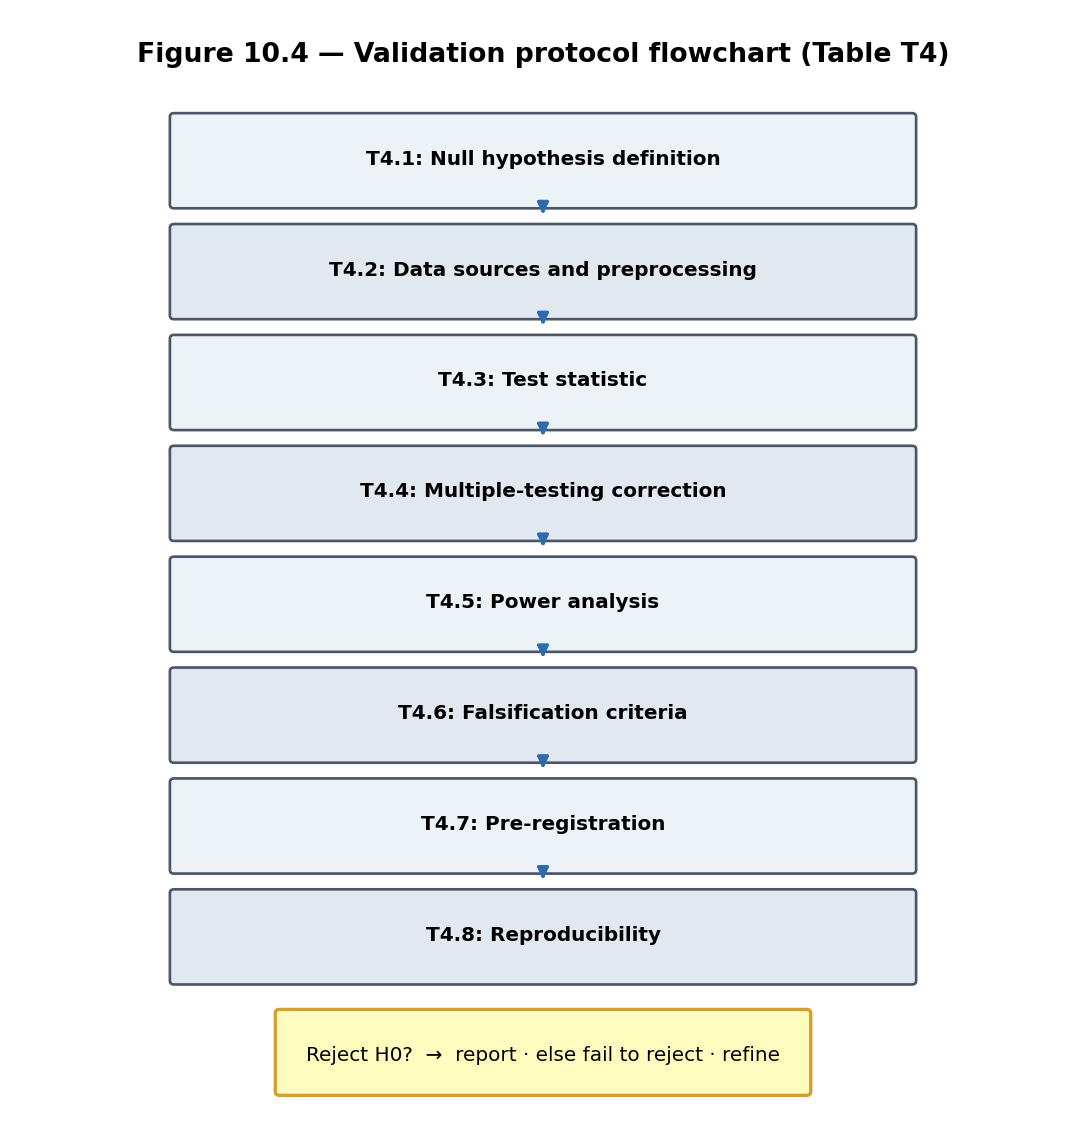
\includegraphics[width=0.92\textwidth,height=0.42\textheight,keepaspectratio]{fig10_4_validation_flowchart.png}
  \caption{Figure 10.4 --- Validation protocol flowchart.}
  \label{fig:fig10-4-validation-flowchart}
\end{figure}

\begin{quote}\small\textit{Figure 10.4.* High-level Table T4 decision tree (details in Appendix D).}\end{quote}

\textbf{Claim type.} Existence of the protocol and helpers: \textbf{Software fact}. ``Hypothesis \(X\) passed T4``: \textbf{Hypothesis} until the full checklist is executed and reviewed.

\textbf{Open Problem 5.} Derive \(W_g=350/\pi\) from lattice geometry, \textbf{or} falsify multi-domain recurrence via pre-registered tests (Appendix D / Table T4).

\bigskip
\noindent\rule{\textwidth}{0.4pt}
\bigskip

\section{10.6 Summary of the entire construction}
\label{ch:ch10_observations:10-6-summary-of-the-entire-construction}

\textbf{Parts I--II (Chapters 1--4)} built the geometric foundation: quaternions, the Hopf fibration, the gauged Hopf lattice, and its symmetries---the higher-dimensional lift of Hatcher's Farey diagram.

\textbf{Part III (Chapters 5--7)} developed the visual and representation-theoretic core: flux topographs, classification and Magic Islands, and the \(Z\mapsto\) flux map.

\textbf{Part IV (Chapters 8--9)} supplied arithmetic depth: composition, class-group analogues, and quaternion algebra / ideal theory as a rigorous home for those analogues. Section 9.5 added a controlled lesson on \textbf{modulus invariants}---algebraic cleanness (e.g.\textbackslash{} \(m=37\)), sequential label progression (often \(m=111\) under coupled step), and true angle--label lock only under explicit angular binning---so that arithmetic labels are never confused with geometric locking.

\textbf{Part V (this chapter)} returns to observation and validation, closing the loop between geometry, arithmetic, and empirical patterns.

Every major claim is labeled so readers can separate theorems, models, and hypotheses; every observational pattern should also name the \textbf{invariant layer} it claims (section 9.5; Table T4).

\bigskip
\noindent\rule{\textwidth}{0.4pt}
\bigskip

\section{10.7 Outlook and invitation}
\label{ch:ch10_observations:10-7-outlook-and-invitation}

The six Open Problems are the main research edges. Advances on \textbf{OP1} (canonical adjacency), \textbf{OP2} (topograph axioms), or \textbf{OP6} (associative composition via ideal theory) especially strengthen the whole framework.

Validation can proceed incrementally: a documented failure to reject the null for \(350/\pi\) in one domain, or a refined class-number invariant with better island prediction, both count as progress. Apply the same null-first discipline as Chapter 9 section 9.5: if a claim is \emph{lock} or \emph{recurrence}, define the null; if it is \emph{algebraic structure}, report the discrete object; if it is \emph{Model flow}, say so and do not upgrade it to geometry by rhetoric.

The \href{https://github.com/kinaar8340/qga}{qga} repository and Kingdom Come portal remain open for extension. \textbf{Book Mode} is live in the portal (chapter map \(\rightarrow\) Hopf / Lattice / Flux / Observations mini demos and tab jumps; see \texttt{HOW\_\allowbreak{}TO\_\allowbreak{}USE.\allowbreak{}md} ?6). Future work includes fuller composition / validation dashboards.

\bigskip
\noindent\rule{\textwidth}{0.4pt}
\bigskip

\section{Exercises (final chapter)}
\label{ch:ch10_observations:exercises-final-chapter}

\textbf{10.A (hand).} Using \textbf{Appendix B}, choose OP1, OP2, or OP6 and write a one-page research proposal: sandbox, diagnostic, and success criterion.

\textbf{10.B (code).} Using \textbf{Appendix D} / \texttt{run\_\allowbreak{}table\_\allowbreak{}t4\_\allowbreak{}demo}, run under the null toy generator and with hand-chosen \(p\)-values. Report Bonferroni threshold, Fisher combined \(p\), and decision. Toy data are \textbf{not} evidence for \(350/\pi\).

\textbf{10.C (code).} Using \texttt{proximity\_\allowbreak{}to\_\allowbreak{}wg} (Appendix D), measure closeness of a few constants to \(350/\pi\). Diagnostic only, not a significance test.

\textbf{10.D (forward).} If OP6 were solved with an associative law from ideal multiplication, what new prediction about Magic Islands or the \(Z\mapsto\) map could be tested under Table T4?

\textbf{10.E (philosophical).} In one paragraph, explain why Theorem / Model / Hypothesis labeling is essential for a project at the intersection of pure mathematics and speculative physics.

\textbf{10.F (project).} Open \texttt{default\_\allowbreak{}hypotheses()} and add one new \texttt{HypothesisSpec} for a domain you care about, with null, falsification, and data sources.

\textbf{10.G (invariant discipline).} Using the three-layer table in this chapter's claim discipline (from Chapter 9 section 9.5), classify each of the following as algebraic / sequential-Model / statistical-lock (or mixed), and name one null or control you would demand: (i) Hurwitz class number 1; (ii) Magic Island high \texttt{stability\_\allowbreak{}score} band; (iii) multi-domain recurrence of \(350/\pi\); (iv) visual ``symmetry'' of a step-index vortex plot.

\bigskip
\noindent\rule{\textwidth}{0.4pt}
\bigskip

\section{Code and asset pointers}
\label{ch:ch10_observations:code-and-asset-pointers}

\begin{lstlisting}[style=qga]
qga/lib/validation.py
Appendix B (Open Problems) ? Appendix D (Table T4 full)
Appendix C ?C.4 (lab listings)
kingdom/observations/ ? kingdom.core.flux_flywheel
\end{lstlisting}

\textbf{Figures:} \texttt{scripts/\allowbreak{}generate\_\allowbreak{}ch10\_\allowbreak{}figures.\allowbreak{}py} \(\cdot\) \textbf{Appendix E} (atlas) \textbf{Related portal:} Observations tab; Flux Flywheel.

\bigskip
\noindent\rule{\textwidth}{0.4pt}
\bigskip

\section{Closing}
\label{ch:ch10_observations:closing}

This book has attempted to lift Allen Hatcher's visual, geometric approach to number theory into the richer world of quaternions and the Hopf fibration, while labeling every claim carefully. The result is a coherent framework connecting classical number theory, topology, and a speculative model of emergent physics.

Whether the Model survives empirical scrutiny is now a question for systematic validation. The tools in Chapters 1--9 and the protocols in this chapter are designed to make that question answerable.

\bigskip
\noindent\rule{\textwidth}{0.4pt}
\bigskip




% ---------- Back matter ----------
\backmatter

\chapter*{Open Problems}
\addcontentsline{toc}{chapter}{Open Problems}
\label{ch:open-problems}
\noindent
The living research edges of the project (see also \texttt{notes/open\_problems.md} in the repository):

\begin{enumerate}[leftmargin=*]
  \item \textbf{OP1 --- Canonical quaternionic Farey structure} (Ch.~\ref{ch:ch03_lattice}).
  \item \textbf{OP2 --- Flux topograph axioms} (Ch.~\ref{ch:ch05_topographs}).
  \item \textbf{OP3 --- Class number \(\leftrightarrow\) Magic Island} (Ch.~\ref{ch:ch06_classification}).
  \item \textbf{OP4 --- \(Z\to\) flywheel uniqueness} (Ch.~\ref{ch:ch07_z_map} / Ch.~\ref{ch:ch10_observations}).
  \item \textbf{OP5 --- \(350/\pi\) first principles or falsification} (Ch.~\ref{ch:ch10_observations}, Table~T4).
  \item \textbf{OP6 --- Composition of flywheels (Gauss lift)} (Ch.~\ref{ch:ch08_class_group}--\ref{ch:ch09_algebras}).
\end{enumerate}

\chapter*{Bibliography (seed)}
\addcontentsline{toc}{chapter}{Bibliography (seed)}
\begin{itemize}[leftmargin=*]
  \item Allen Hatcher, \emph{Topology of Numbers}, AMS, 2022.
        Free PDF: \url{https://pi.math.cornell.edu/~hatcher/TN/TNbook.pdf}.
  \item Classical quaternion arithmetic: Hurwitz; Conway--Smith, \emph{On Quaternions and Octonions}.
  \item Quaternion algebras: Vignéras; Voight, \emph{Quaternion Algebras}.
  \item Hopf fibration surveys; topological phases / monopoles literature.
  \item Kingdom Come repository and observation program:
        \url{https://github.com/kinaar8340/kingdom_come}.
  \item This book repository: \url{https://github.com/kinaar8340/qga}.
\end{itemize}

\end{document}
